\documentclass[twoside]{book}

% Packages required by doxygen
\usepackage{calc}
\usepackage{doxygen}
\usepackage{graphicx}
\usepackage[utf8]{inputenc}
\usepackage{makeidx}
\usepackage{multicol}
\usepackage{multirow}
\usepackage{textcomp}
\usepackage[table]{xcolor}

% Font selection
\usepackage[T1]{fontenc}
\usepackage{mathptmx}
\usepackage[scaled=.90]{helvet}
\usepackage{courier}
\usepackage{amssymb}
\usepackage{sectsty}
\renewcommand{\familydefault}{\sfdefault}
\allsectionsfont{%
  \fontseries{bc}\selectfont%
  \color{darkgray}%
}
\renewcommand{\DoxyLabelFont}{%
  \fontseries{bc}\selectfont%
  \color{darkgray}%
}

% Page & text layout
\usepackage{geometry}
\geometry{%
  a4paper,%
  top=2.5cm,%
  bottom=2.5cm,%
  left=2.5cm,%
  right=2.5cm%
}
\tolerance=750
\hfuzz=15pt
\hbadness=750
\setlength{\emergencystretch}{15pt}
\setlength{\parindent}{0cm}
\setlength{\parskip}{0.2cm}
\makeatletter
\renewcommand{\paragraph}{%
  \@startsection{paragraph}{4}{0ex}{-1.0ex}{1.0ex}{%
    \normalfont\normalsize\bfseries\SS@parafont%
  }%
}
\renewcommand{\subparagraph}{%
  \@startsection{subparagraph}{5}{0ex}{-1.0ex}{1.0ex}{%
    \normalfont\normalsize\bfseries\SS@subparafont%
  }%
}
\makeatother

% Headers & footers
\usepackage{fancyhdr}
\pagestyle{fancyplain}
\fancyhead[LE]{\fancyplain{}{\bfseries\thepage}}
\fancyhead[CE]{\fancyplain{}{}}
\fancyhead[RE]{\fancyplain{}{\bfseries\leftmark}}
\fancyhead[LO]{\fancyplain{}{\bfseries\rightmark}}
\fancyhead[CO]{\fancyplain{}{}}
\fancyhead[RO]{\fancyplain{}{\bfseries\thepage}}
\fancyfoot[LE]{\fancyplain{}{}}
\fancyfoot[CE]{\fancyplain{}{}}
\fancyfoot[RE]{\fancyplain{}{\bfseries\scriptsize Generated on Tue Mar 14 2017 08\-:58\-:35 for A\-S\-C\-O Aerial Autonomy by Doxygen }}
\fancyfoot[LO]{\fancyplain{}{\bfseries\scriptsize Generated on Tue Mar 14 2017 08\-:58\-:35 for A\-S\-C\-O Aerial Autonomy by Doxygen }}
\fancyfoot[CO]{\fancyplain{}{}}
\fancyfoot[RO]{\fancyplain{}{}}
\renewcommand{\footrulewidth}{0.4pt}
\renewcommand{\chaptermark}[1]{%
  \markboth{#1}{}%
}
\renewcommand{\sectionmark}[1]{%
  \markright{\thesection\ #1}%
}

% Indices & bibliography
\usepackage{natbib}
\usepackage[titles]{tocloft}
\setcounter{tocdepth}{3}
\setcounter{secnumdepth}{5}
\makeindex

% Hyperlinks (required, but should be loaded last)
\usepackage{ifpdf}
\ifpdf
  \usepackage[pdftex,pagebackref=true]{hyperref}
\else
  \usepackage[ps2pdf,pagebackref=true]{hyperref}
\fi
\hypersetup{%
  colorlinks=true,%
  linkcolor=blue,%
  citecolor=blue,%
  unicode%
}

% Custom commands
\newcommand{\clearemptydoublepage}{%
  \newpage{\pagestyle{empty}\cleardoublepage}%
}


%===== C O N T E N T S =====

\begin{document}

% Titlepage & ToC
\hypersetup{pageanchor=false}
\pagenumbering{roman}
\begin{titlepage}
\vspace*{7cm}
\begin{center}%
{\Large A\-S\-C\-O Aerial Autonomy }\\
\vspace*{1cm}
{\large Generated by Doxygen 1.8.6}\\
\vspace*{0.5cm}
{\small Tue Mar 14 2017 08:58:35}\\
\end{center}
\end{titlepage}
\clearemptydoublepage
\tableofcontents
\clearemptydoublepage
\pagenumbering{arabic}
\hypersetup{pageanchor=true}

%--- Begin generated contents ---
\chapter{Main Page}
\label{index}\hypertarget{index}{}\section*{Background}

\subsection*{Goal}

Easily create autonomy applications by combining modular state behaviors into domain-\/specific state machines. Use generic interfaces for quadcopter and manipulator hardware which allow users to adapt existing hardware drivers to the framework.

\section*{Project}

The goal of the project is to create a generic state machine interface for the quadrotor and arm to do different tasks such as “pick and place”, “screwing a lightbulb”, “\-A\-R manipulation”, etc. This requires different types of controllers, estimators and state logic based on the task at hand. The framework consists of the following main components\-:


\begin{DoxyEnumerate}
\item Robot System
\begin{DoxyEnumerate}
\item Controllers
\item Hardware Plugins
\item Estimators
\item Controller\-Hardware\-Interfaces
\end{DoxyEnumerate}
\item \hyperlink{classLogicStateMachineFrontEnd}{Logic\-State\-Machine\-Front\-End}
\item \hyperlink{classStateMachineGUIConnector}{State\-Machine\-G\-U\-I\-Connector}
\item G\-U\-I\-Front\-End
\item \hyperlink{classOnboardSystemHandler}{Onboard\-System\-Handler}
\end{DoxyEnumerate}

\section*{Components}

\subsection*{Robot System}

The robot system owns privately the hardware, controllers, estimators and controller-\/hardware interfaces. For the public interface it provides methods to retrieve sensor/estimator data, and select and set controller goals for the robot.

\begin{TabularC}{3}
\hline
\rowcolor{lightgray}{\bf Component }&{\bf Description }&{\bf Link  }\\\cline{1-3}
Hardware &Send commands to hardware and retrieve raw sensor data &\hyperlink{classUAVSystem}{U\-A\-V\-System} \\\cline{1-3}
Controllers &Provide run function that returns the controls to send back to hardware based on sensor data &\hyperlink{classBuiltInController}{Built\-In\-Controller} \\\cline{1-3}
Estimators &Compute the robot state/parameters based on raw sensor data &None \\\cline{1-3}
Controller-\/\-Hardware Interfaces &For a single controller, extracts sensor/estimator data from hardware, passes it to the controller run function, and sends the resulting control commands to hardware &\hyperlink{classControllerHardwareConnector}{Controller\-Hardware\-Connector} \\\cline{1-3}
\end{TabularC}
\subsection*{Logic State Machine (\hyperlink{classLogicStateMachineFrontEnd}{Logic\-State\-Machine\-Front\-End})}

The Logic State Machine (L\-S\-M) contains the behavior necessary to achieve a desired task. Each state in a logic state machine contains a {\ttfamily run} function that executes state-\/specific behaviors and triggers appropriate state transitions. The L\-S\-M behavior is executed at a user-\/defined frequency



The L\-S\-M also provides a sub state machine for checking the health of the hardware based on sensor data, and health reported by the hardware plugins. The state of this submachine is used to guard the transitions between different states. For example, if the quadrotor has a low battery warning, the quadrotor will not accept a goal command to fly to a goal far away. If the battery level is critical, the health sub machine may trigger a land event automatically.

\subsection*{\hyperlink{classStateMachineGUIConnector}{State\-Machine\-G\-U\-I\-Connector}}

The \hyperlink{classStateMachineGUIConnector}{State\-Machine\-G\-U\-I\-Connector} connects the G\-U\-I interface to the state machine. It provides a message based interface for triggering manual state transitions through the G\-U\-I. These actions can be very generic -\/ such as buttons for “start mission” and “start tracking” -\/ and can be specific such as “land”.

\subsection*{G\-U\-I\-Front\-End (\hyperlink{classaerial__autonomy_1_1aerial__autonomy__gui_1_1EventTransmissionGUI}{aerial\-\_\-autonomy.\-aerial\-\_\-autonomy\-\_\-gui.\-Event\-Transmission\-G\-U\-I})}

The G\-U\-I contains a text box that updates the status of all the hardware plugins and the state machine. The status of the hardware plugins include the health information of the hardware and the state of the hardware in the world. The state machine status includes information about the current state and any events that are not accepted by the state machine. In addition, the G\-U\-I should be able to send manual triggers to the state machine that are generated by the user. Here is an example G\-U\-I Front\-End\-:

\begin{DoxyRefDesc}{Todo}
\item[\hyperlink{todo__todo000014}{Todo}]Add picture of latest G\-U\-I with quad status etc\end{DoxyRefDesc}


The Triggers should be connected to the {\ttfamily State\-Machine} using {\ttfamily \hyperlink{classStateMachineGUIConnector}{State\-Machine\-G\-U\-I\-Connector}} class. The triggers are events without any information. There can also be commands with information using {\ttfamily Rviz} goalpose callbacks to send the drone to a specific location.

\subsection*{Classes segregated into groups}

The classes created in this project can be found \hyperlink{md_markdown_scripts_class_groups}{here} 
\chapter{Classes by Group}
\label{md_markdown_scripts_class_groups}
\hypertarget{md_markdown_scripts_class_groups}{}
\subsection*{Controllers}


\begin{DoxyItemize}
\item \hyperlink{classBuiltInController}{Built\-In\-Controller}
\item \hyperlink{classManualRPYTController}{Manual\-R\-P\-Y\-T\-Controller}
\end{DoxyItemize}

\subsection*{Controller\-Hardware\-Connectors}


\begin{DoxyItemize}
\item \hyperlink{structAbstractControllerHardwareConnector}{Abstract\-Controller\-Hardware\-Connector}
\begin{DoxyItemize}
\item \hyperlink{classControllerHardwareConnector}{Controller\-Hardware\-Connector}
\begin{DoxyItemize}
\item \hyperlink{classBuiltInVelocityControllerDroneConnector}{Built\-In\-Velocity\-Controller\-Drone\-Connector}
\item \hyperlink{classPositionControllerDroneConnector}{Position\-Controller\-Drone\-Connector}
\item \hyperlink{classManualRPYTControllerDroneConnector}{Manual\-R\-P\-Y\-T\-Controller\-Drone\-Connector}
\end{DoxyItemize}
\end{DoxyItemize}
\end{DoxyItemize}

\subsection*{States}


\begin{DoxyItemize}
\item \hyperlink{classBaseState}{Base\-State}
\begin{DoxyItemize}
\item \hyperlink{structLogicStateMachineFrontEnd_1_1Landed}{Logic\-State\-Machine\-Front\-End\-::\-Landed}
\item \hyperlink{takeoff__functors_8h_ab6710f3cb12b7653eedcd3a2215d3228}{Taking\-Off\-\_\-}
\item \hyperlink{hovering__functors_8h_a4252f403b3bcd2a850cf271512d9c6ff}{Hovering\-\_\-}
\item \hyperlink{position__control__functors_8h_af380346c24b534da18813f70217ea50f}{Reaching\-Goal\-\_\-}
\item \hyperlink{land__functors_8h_a84627965433a60de431758bddec005c3}{Landing\-\_\-}
\end{DoxyItemize}
\end{DoxyItemize}

\subsection*{Action Functors}


\begin{DoxyItemize}
\item \hyperlink{structActionFunctor}{Action\-Functor}
\begin{DoxyItemize}
\item \hyperlink{structLandTransitionActionFunctor__}{Land\-Transition\-Action\-Functor\-\_\-}
\item \hyperlink{structTakeoffTransitionActionFunctor__}{Takeoff\-Transition\-Action\-Functor\-\_\-}
\item \hyperlink{structPositionControlTransitionActionFunctor__}{Position\-Control\-Transition\-Action\-Functor\-\_\-}
\end{DoxyItemize}
\item \hyperlink{structEventAgnosticActionFunctor}{Event\-Agnostic\-Action\-Functor}
\begin{DoxyItemize}
\item \hyperlink{structLandInternalActionFunctor__}{Land\-Internal\-Action\-Functor\-\_\-}
\item \hyperlink{structTakeoffInternalActionFunctor__}{Takeoff\-Internal\-Action\-Functor\-\_\-}
\item \hyperlink{structTakeoffAbortActionFunctor__}{Takeoff\-Abort\-Action\-Functor\-\_\-}
\item \hyperlink{structHoveringInternalActionFunctor__}{Hovering\-Internal\-Action\-Functor\-\_\-}
\item \hyperlink{structPositionControlAbortActionFunctor__}{Position\-Control\-Abort\-Action\-Functor\-\_\-}
\item \hyperlink{structPositionControlInternalActionFunctor__}{Position\-Control\-Internal\-Action\-Functor\-\_\-}
\end{DoxyItemize}
\end{DoxyItemize}

\subsection*{Guard Functors}


\begin{DoxyItemize}
\item \hyperlink{structGuardFunctor}{Guard\-Functor}
\begin{DoxyItemize}
\item \hyperlink{structTakeoffTransitionGuardFunctor__}{Takeoff\-Transition\-Guard\-Functor\-\_\-}
\item \hyperlink{structPositionControlTransitionGuardFunctor__}{Position\-Control\-Transition\-Guard\-Functor\-\_\-}
\end{DoxyItemize}
\item \hyperlink{structEventAgnosticGuardFunctor}{Event\-Agnostic\-Guard\-Functor}
\end{DoxyItemize}

\subsection*{State Machine Front End}


\begin{DoxyItemize}
\item \hyperlink{classLogicStateMachineFrontEnd}{Logic\-State\-Machine\-Front\-End}
\end{DoxyItemize}

\subsection*{State Machine Back End}


\begin{DoxyItemize}
\item \hyperlink{basic__state__machine_8h_ab0b6ef21baf57684550a2f05c771bd86}{Logic\-State\-Machine}
\end{DoxyItemize}

\subsection*{Robot Systems}


\begin{DoxyItemize}
\item \hyperlink{classUAVSystem}{U\-A\-V\-System} 
\end{DoxyItemize}
\chapter{Creating a State Machine}
\label{md_markdown_scripts_creating_state_machine}
\hypertarget{md_markdown_scripts_creating_state_machine}{}
To create a state machine, we need to implement the following components\-:

\begin{TabularC}{2}
\hline
\rowcolor{lightgray}{\bf Component }&{\bf Description  }\\\cline{1-2}
Robot system &Provides sensor data and accepts control commands \\\cline{1-2}
Actions &Commands to execute when switching between states \\\cline{1-2}
Guards &Check if the transition between states is valid or not \\\cline{1-2}
Internal actions &Process robot state continuously and trigger actions accordingly \\\cline{1-2}
\end{TabularC}


\subsection*{Creating a robot system}

\begin{DoxyRefDesc}{Todo}
\item[\hyperlink{todo__todo000015}{Todo}](Matt) Fill this page \end{DoxyRefDesc}

\chapter{Todo List}
\label{todo}
\hypertarget{todo}{}

\begin{DoxyRefList}
\item[\label{todo__todo000001}%
\hypertarget{todo__todo000001}{}%
Member \hyperlink{classaerial__autonomy_1_1aerial__autonomy__gui_1_1EventTransmissionGUI_a6118098a267761831ef8d83cbf2a78bd}{aerial\-\_\-autonomy.aerial\-\_\-autonomy\-\_\-gui.Event\-Transmission\-G\-U\-I.height\-\_\-slider} ]Matt\-: Load slider settings from param file  
\item[\label{todo__todo000002}%
\hypertarget{todo__todo000002}{}%
Member \hyperlink{classaerial__autonomy_1_1aerial__autonomy__gui_1_1EventTransmissionGUI_af611df98da28aba90ce5fcbea285603a}{aerial\-\_\-autonomy.aerial\-\_\-autonomy\-\_\-gui.Event\-Transmission\-G\-U\-I.pose\-\_\-command\-\_\-container} ]Matt\-: Reset slider value based on current quad height  
\item[\label{todo__todo000015}%
\hypertarget{todo__todo000015}{}%
Page \hyperlink{md_markdown_scripts_creating_state_machine}{Creating a State Machine} ](Matt) Fill this page  
\item[\label{todo__todo000005}%
\hypertarget{todo__todo000005}{}%
Member \hyperlink{structHoveringInternalActionFunctor___a87bb8dd8ed71e54729967b9e258fb66e}{Hovering\-Internal\-Action\-Functor\-\_\-$<$ Logic\-State\-Machine\-T $>$\-:\-:run} (\hyperlink{classUAVSystem}{U\-A\-V\-System} \&robot\-\_\-system, Logic\-State\-Machine\-T \&logic\-\_\-state\-\_\-machine)](Gowtham) Can also use uav status here  
\item[\label{todo__todo000006}%
\hypertarget{todo__todo000006}{}%
Class \hyperlink{structLandInternalActionFunctor__}{Land\-Internal\-Action\-Functor\-\_\-$<$ Logic\-State\-Machine\-T $>$} ](Gowtham) How to abort Land?? 
\item[\label{todo__todo000008}%
\hypertarget{todo__todo000008}{}%
Member \hyperlink{structLandInternalActionFunctor___a4557b02d6cfa6712b610337cb606f54b}{Land\-Internal\-Action\-Functor\-\_\-$<$ Logic\-State\-Machine\-T $>$\-:\-:run} (\hyperlink{classUAVSystem}{U\-A\-V\-System} \&robot\-\_\-system, Logic\-State\-Machine\-T \&logic\-\_\-state\-\_\-machine)](Gowtham) Can also use uav status here  
\item[\label{todo__todo000007}%
\hypertarget{todo__todo000007}{}%
Member \hyperlink{structLandTransitionActionFunctor___ae91b354f041edda283e306fa312e1213}{Land\-Transition\-Action\-Functor\-\_\-$<$ Logic\-State\-Machine\-T $>$\-:\-:run} (\hyperlink{classUAVSystem}{U\-A\-V\-System} \&robot\-\_\-system, Logic\-State\-Machine\-T \&)]Have to abort all hardware controllers not just U\-A\-V.  
\item[\label{todo__todo000014}%
\hypertarget{todo__todo000014}{}%
page \hyperlink{index}{Main Page} ]Add picture of latest G\-U\-I with quad status etc 
\item[\label{todo__todo000003}%
\hypertarget{todo__todo000003}{}%
Member \hyperlink{classManualRPYTController_ae29c56af6d0bc913d357c7849201c8fb}{Manual\-R\-P\-Y\-T\-Controller\-:\-:run\-Implementation} (\hyperlink{structJoysticksYaw}{Joysticks\-Yaw} sensor\-\_\-data, \hyperlink{structEmptyGoal}{Empty\-Goal} goal)](matt)\-: need to pass R\-C mapping as parameter 

(matt)\-: need to pass in frequency as a parameter  
\item[\label{todo__todo000009}%
\hypertarget{todo__todo000009}{}%
Class \hyperlink{structPositionControlTransitionGuardFunctor__}{Position\-Control\-Transition\-Guard\-Functor\-\_\-$<$ Logic\-State\-Machine\-T $>$} ]Use a parameter for setting position tolerance 
\item[\label{todo__todo000013}%
\hypertarget{todo__todo000013}{}%
Member \hyperlink{classSystemStatusPublisher_a66f73a2e489face69d6f9fc16abb15aa}{System\-Status\-Publisher$<$ Logic\-State\-Machine\-T $>$\-:\-:publish\-System\-Status} ()]Replace status text with html script. Need a html manager to automatically add table lines  
\item[\label{todo__todo000010}%
\hypertarget{todo__todo000010}{}%
Member \hyperlink{structTakeoffInternalActionFunctor___a2118df6e326662cd0088344499e49696}{Takeoff\-Internal\-Action\-Functor\-\_\-$<$ Logic\-State\-Machine\-T $>$\-:\-:run} (\hyperlink{classUAVSystem}{U\-A\-V\-System} \&robot\-\_\-system, Logic\-State\-Machine\-T \&logic\-\_\-state\-\_\-machine)]add a parameter for height when to transition from takeoff to hovering 
\item[\label{todo__todo000012}%
\hypertarget{todo__todo000012}{}%
Member \hyperlink{classUAVSystem_a9218f794905e832cc356b5e4b659e1da}{U\-A\-V\-System\-:\-:U\-A\-V\-System} (parsernode\-::\-Parser \&drone\-\_\-hardware, U\-A\-V\-System\-Config config)]make enum class iterable to do this automatically 
\end{DoxyRefList}
\chapter{Namespace Index}
\section{Namespace List}
Here is a list of all namespaces with brief descriptions\-:\begin{DoxyCompactList}
\item\contentsline{section}{\hyperlink{namespaceaerial__autonomy}{aerial\-\_\-autonomy} \\*G\-U\-I source code to provide user the ability to trigger events from G\-U\-I to state machine }{\pageref{namespaceaerial__autonomy}}{}
\item\contentsline{section}{\hyperlink{namespaceaerial__autonomy_1_1aerial__autonomy__gui}{aerial\-\_\-autonomy.\-aerial\-\_\-autonomy\-\_\-gui} \\*Generate a G\-U\-I to trigger events for state machine }{\pageref{namespaceaerial__autonomy_1_1aerial__autonomy__gui}}{}
\item\contentsline{section}{\hyperlink{namespaceaerial__autonomy_1_1ros__event__trigger}{aerial\-\_\-autonomy.\-ros\-\_\-event\-\_\-trigger} \\*Ros connection between G\-U\-I and state machine }{\pageref{namespaceaerial__autonomy_1_1ros__event__trigger}}{}
\item\contentsline{section}{\hyperlink{namespaceboost}{boost} \\*Boost namespace }{\pageref{namespaceboost}}{}
\item\contentsline{section}{\hyperlink{namespaceboost_1_1msm}{boost\-::msm} \\*Meta state machine namespace }{\pageref{namespaceboost_1_1msm}}{}
\item\contentsline{section}{\hyperlink{namespaceboost_1_1msm_1_1back}{boost\-::msm\-::back} \\*Backend namespace }{\pageref{namespaceboost_1_1msm_1_1back}}{}
\end{DoxyCompactList}

\chapter{Hierarchical Index}
\section{Class Hierarchy}
This inheritance list is sorted roughly, but not completely, alphabetically\-:\begin{DoxyCompactList}
\item \contentsline{section}{Abstract\-Controller\-Hardware\-Connector}{\pageref{structAbstractControllerHardwareConnector}}{}
\begin{DoxyCompactList}
\item \contentsline{section}{Controller\-Hardware\-Connector$<$ Sensor\-Data\-Type, Goal\-Type, Control\-Type $>$}{\pageref{classControllerHardwareConnector}}{}
\item \contentsline{section}{Controller\-Hardware\-Connector$<$ Empty\-Sensor, Position\-Yaw, Position\-Yaw $>$}{\pageref{classControllerHardwareConnector}}{}
\begin{DoxyCompactList}
\item \contentsline{section}{Position\-Controller\-Drone\-Connector}{\pageref{classPositionControllerDroneConnector}}{}
\end{DoxyCompactList}
\item \contentsline{section}{Controller\-Hardware\-Connector$<$ Empty\-Sensor, Velocity\-Yaw, Velocity\-Yaw $>$}{\pageref{classControllerHardwareConnector}}{}
\begin{DoxyCompactList}
\item \contentsline{section}{Built\-In\-Velocity\-Controller\-Drone\-Connector}{\pageref{classBuiltInVelocityControllerDroneConnector}}{}
\end{DoxyCompactList}
\item \contentsline{section}{Controller\-Hardware\-Connector$<$ Joysticks\-Yaw, Empty\-Goal, Roll\-Pitch\-Yaw\-Thrust $>$}{\pageref{classControllerHardwareConnector}}{}
\begin{DoxyCompactList}
\item \contentsline{section}{Manual\-R\-P\-Y\-T\-Controller\-Drone\-Connector}{\pageref{classManualRPYTControllerDroneConnector}}{}
\end{DoxyCompactList}
\end{DoxyCompactList}
\item \contentsline{section}{Action\-Functor$<$ Event\-T, Robot\-System\-T, Logic\-State\-Machine\-T $>$}{\pageref{structActionFunctor}}{}
\item \contentsline{section}{Action\-Functor$<$ Position\-Yaw, U\-A\-V\-System, Logic\-State\-Machine\-T $>$}{\pageref{structActionFunctor}}{}
\begin{DoxyCompactList}
\item \contentsline{section}{Position\-Control\-Transition\-Action\-Functor\-\_\-$<$ Logic\-State\-Machine\-T $>$}{\pageref{structPositionControlTransitionActionFunctor__}}{}
\end{DoxyCompactList}
\item \contentsline{section}{Async\-Timer}{\pageref{classAsyncTimer}}{}
\item \contentsline{section}{Completed}{\pageref{structCompleted}}{}
\item \contentsline{section}{Controller$<$ Sensor\-Data\-Type, Goal\-Type, Control\-Type $>$}{\pageref{classController}}{}
\item \contentsline{section}{Controller$<$ Empty\-Sensor, Goal\-Type, Goal\-Type $>$}{\pageref{classController}}{}
\begin{DoxyCompactList}
\item \contentsline{section}{Built\-In\-Controller$<$ Goal\-Type $>$}{\pageref{classBuiltInController}}{}
\end{DoxyCompactList}
\item \contentsline{section}{Controller$<$ Empty\-Sensor, Position\-Yaw, Position\-Yaw $>$}{\pageref{classController}}{}
\begin{DoxyCompactList}
\item \contentsline{section}{Built\-In\-Controller$<$ Position\-Yaw $>$}{\pageref{classBuiltInController}}{}
\end{DoxyCompactList}
\item \contentsline{section}{Controller$<$ Empty\-Sensor, Velocity\-Yaw, Velocity\-Yaw $>$}{\pageref{classController}}{}
\begin{DoxyCompactList}
\item \contentsline{section}{Built\-In\-Controller$<$ Velocity\-Yaw $>$}{\pageref{classBuiltInController}}{}
\end{DoxyCompactList}
\item \contentsline{section}{Controller$<$ Joysticks\-Yaw, Empty\-Goal, Roll\-Pitch\-Yaw\-Thrust $>$}{\pageref{classController}}{}
\begin{DoxyCompactList}
\item \contentsline{section}{Manual\-R\-P\-Y\-T\-Controller}{\pageref{classManualRPYTController}}{}
\end{DoxyCompactList}
\item \contentsline{section}{Empty\-Goal}{\pageref{structEmptyGoal}}{}
\item \contentsline{section}{Empty\-Robot\-System}{\pageref{structEmptyRobotSystem}}{}
\item \contentsline{section}{Empty\-Sensor}{\pageref{structEmptySensor}}{}
\item \contentsline{section}{Event\-Agnostic\-Action\-Functor$<$ Robot\-System\-T, Logic\-State\-Machine\-T $>$}{\pageref{structEventAgnosticActionFunctor}}{}
\item \contentsline{section}{Event\-Agnostic\-Action\-Functor$<$ U\-A\-V\-System, Logic\-State\-Machine\-T $>$}{\pageref{structEventAgnosticActionFunctor}}{}
\begin{DoxyCompactList}
\item \contentsline{section}{Hovering\-Internal\-Action\-Functor\-\_\-$<$ Logic\-State\-Machine\-T $>$}{\pageref{structHoveringInternalActionFunctor__}}{}
\item \contentsline{section}{Land\-Internal\-Action\-Functor\-\_\-$<$ Logic\-State\-Machine\-T $>$}{\pageref{structLandInternalActionFunctor__}}{}
\item \contentsline{section}{Land\-Transition\-Action\-Functor\-\_\-$<$ Logic\-State\-Machine\-T $>$}{\pageref{structLandTransitionActionFunctor__}}{}
\item \contentsline{section}{Position\-Control\-Abort\-Action\-Functor\-\_\-$<$ Logic\-State\-Machine\-T $>$}{\pageref{structPositionControlAbortActionFunctor__}}{}
\item \contentsline{section}{Position\-Control\-Internal\-Action\-Functor\-\_\-$<$ Logic\-State\-Machine\-T $>$}{\pageref{structPositionControlInternalActionFunctor__}}{}
\item \contentsline{section}{Takeoff\-Abort\-Action\-Functor\-\_\-$<$ Logic\-State\-Machine\-T $>$}{\pageref{structTakeoffAbortActionFunctor__}}{}
\item \contentsline{section}{Takeoff\-Internal\-Action\-Functor\-\_\-$<$ Logic\-State\-Machine\-T $>$}{\pageref{structTakeoffInternalActionFunctor__}}{}
\item \contentsline{section}{Takeoff\-Transition\-Action\-Functor\-\_\-$<$ Logic\-State\-Machine\-T $>$}{\pageref{structTakeoffTransitionActionFunctor__}}{}
\end{DoxyCompactList}
\item \contentsline{section}{Event\-Agnostic\-Guard\-Functor$<$ Robot\-System\-T, Logic\-State\-Machine\-T $>$}{\pageref{structEventAgnosticGuardFunctor}}{}
\item \contentsline{section}{Event\-Agnostic\-Guard\-Functor$<$ U\-A\-V\-System, Logic\-State\-Machine\-T $>$}{\pageref{structEventAgnosticGuardFunctor}}{}
\begin{DoxyCompactList}
\item \contentsline{section}{Takeoff\-Transition\-Guard\-Functor\-\_\-$<$ Logic\-State\-Machine\-T $>$}{\pageref{structTakeoffTransitionGuardFunctor__}}{}
\end{DoxyCompactList}
\item \contentsline{section}{Event\-Publisher}{\pageref{classEventPublisher}}{}
\item \contentsline{section}{Guard\-Functor$<$ Event\-T, Robot\-System\-T, Logic\-State\-Machine\-T $>$}{\pageref{structGuardFunctor}}{}
\item \contentsline{section}{Guard\-Functor$<$ Position\-Yaw, U\-A\-V\-System, Logic\-State\-Machine\-T $>$}{\pageref{structGuardFunctor}}{}
\begin{DoxyCompactList}
\item \contentsline{section}{Position\-Control\-Transition\-Guard\-Functor\-\_\-$<$ Logic\-State\-Machine\-T $>$}{\pageref{structPositionControlTransitionGuardFunctor__}}{}
\end{DoxyCompactList}
\item \contentsline{section}{Internal\-Transition\-Event}{\pageref{structInternalTransitionEvent}}{}
\item \contentsline{section}{Joysticks}{\pageref{structJoysticks}}{}
\begin{DoxyCompactList}
\item \contentsline{section}{Joysticks\-Yaw}{\pageref{structJoysticksYaw}}{}
\end{DoxyCompactList}
\item \contentsline{section}{Onboard\-System\-Handler$<$ Logic\-State\-Machine\-T, Event\-Manager\-T $>$}{\pageref{classOnboardSystemHandler}}{}
\item Parser\begin{DoxyCompactList}
\item \contentsline{section}{Sample\-Parser}{\pageref{classSampleParser}}{}
\end{DoxyCompactList}
\item \contentsline{section}{Position}{\pageref{structPosition}}{}
\begin{DoxyCompactList}
\item \contentsline{section}{Position\-Yaw}{\pageref{structPositionYaw}}{}
\end{DoxyCompactList}
\item \contentsline{section}{Roll\-Pitch\-Yaw\-Thrust}{\pageref{structRollPitchYawThrust}}{}
\item \contentsline{section}{Sample\-Logic\-State\-Machine\-\_\-$<$ Robot\-System\-T $>$}{\pageref{classSampleLogicStateMachine__}}{}
\item state\begin{DoxyCompactList}
\item \contentsline{section}{Base\-State$<$ Robot\-System\-T, Logic\-State\-Machine\-T, Action\-Fctr $>$}{\pageref{classBaseState}}{}
\item \contentsline{section}{Logic\-State\-Machine\-Front\-End\-:\-:Landed}{\pageref{structLogicStateMachineFrontEnd_1_1Landed}}{}
\end{DoxyCompactList}
\item state\-\_\-machine\begin{DoxyCompactList}
\item \contentsline{section}{boost\-:\-:msm\-:\-:back\-:\-:thread\-\_\-safe\-\_\-state\-\_\-machine$<$ A0, A1, A2, A3, A4 $>$}{\pageref{classboost_1_1msm_1_1back_1_1thread__safe__state__machine}}{}
\end{DoxyCompactList}
\item state\-\_\-machine\-\_\-def\begin{DoxyCompactList}
\item \contentsline{section}{Logic\-State\-Machine\-Front\-End}{\pageref{classLogicStateMachineFrontEnd}}{}
\end{DoxyCompactList}
\item \contentsline{section}{State\-Machine\-G\-U\-I\-Connector$<$ Event\-Manager\-T, Logic\-State\-Machine\-T $>$}{\pageref{classStateMachineGUIConnector}}{}
\item \contentsline{section}{System\-Status\-Publisher$<$ Logic\-State\-Machine\-T $>$}{\pageref{classSystemStatusPublisher}}{}
\item \contentsline{section}{Type\-Map$<$ Generic\-Object\-T $>$}{\pageref{classTypeMap}}{}
\item \contentsline{section}{Type\-Map$<$ Abstract\-Controller\-Hardware\-Connector $>$}{\pageref{classTypeMap}}{}
\item \contentsline{section}{U\-A\-V\-System}{\pageref{classUAVSystem}}{}
\item vector\begin{DoxyCompactList}
\item \contentsline{section}{Base\-State$<$ Robot\-System\-T, Logic\-State\-Machine\-T, Action\-Fctr $>$\-:\-:internal\-\_\-transition\-\_\-table}{\pageref{structBaseState_1_1internal__transition__table}}{}
\item \contentsline{section}{Logic\-State\-Machine\-Front\-End\-:\-:Landed\-:\-:internal\-\_\-transition\-\_\-table}{\pageref{structLogicStateMachineFrontEnd_1_1Landed_1_1internal__transition__table}}{}
\item \contentsline{section}{Logic\-State\-Machine\-Front\-End\-:\-:transition\-\_\-table}{\pageref{structLogicStateMachineFrontEnd_1_1transition__table}}{}
\end{DoxyCompactList}
\item \contentsline{section}{Velocity}{\pageref{structVelocity}}{}
\begin{DoxyCompactList}
\item \contentsline{section}{Velocity\-Yaw}{\pageref{structVelocityYaw}}{}
\end{DoxyCompactList}
\item Plugin\begin{DoxyCompactList}
\item \contentsline{section}{aerial\-\_\-autonomy.\-aerial\-\_\-autonomy\-\_\-gui.\-Event\-Transmission\-G\-U\-I}{\pageref{classaerial__autonomy_1_1aerial__autonomy__gui_1_1EventTransmissionGUI}}{}
\end{DoxyCompactList}
\item Q\-Object\begin{DoxyCompactList}
\item \contentsline{section}{aerial\-\_\-autonomy.\-ros\-\_\-event\-\_\-trigger.\-Ros\-Event\-Trigger}{\pageref{classaerial__autonomy_1_1ros__event__trigger_1_1RosEventTrigger}}{}
\end{DoxyCompactList}
\end{DoxyCompactList}

\chapter{Class Index}
\section{Class List}
Here are the classes, structs, unions and interfaces with brief descriptions\-:\begin{DoxyCompactList}
\item\contentsline{section}{\hyperlink{structAbstractControllerHardwareConnector}{Abstract\-Controller\-Hardware\-Connector} \\*Base for \hyperlink{classControllerHardwareConnector}{Controller\-Hardware\-Connector} class }{\pageref{structAbstractControllerHardwareConnector}}{}
\item\contentsline{section}{\hyperlink{structActionFunctor}{Action\-Functor$<$ Event\-T, Robot\-System\-T, Logic\-State\-Machine\-T $>$} \\*Action Functor for a given event, robot system, state machine }{\pageref{structActionFunctor}}{}
\item\contentsline{section}{\hyperlink{classAsyncTimer}{Async\-Timer} \\*Calls given function on a timer in its own thread }{\pageref{classAsyncTimer}}{}
\item\contentsline{section}{\hyperlink{classBaseState}{Base\-State$<$ Robot\-System\-T, Logic\-State\-Machine\-T, Action\-Fctr $>$} \\*Base state for all states in logic state machine }{\pageref{classBaseState}}{}
\item\contentsline{section}{\hyperlink{classBuiltInController}{Built\-In\-Controller$<$ Goal\-Type $>$} \\*A controller that simply outputs the set goal }{\pageref{classBuiltInController}}{}
\item\contentsline{section}{\hyperlink{classBuiltInVelocityControllerDroneConnector}{Built\-In\-Velocity\-Controller\-Drone\-Connector} \\*Manages communication between a drone plugin and a velocity controller that outputs velocity commands }{\pageref{classBuiltInVelocityControllerDroneConnector}}{}
\item\contentsline{section}{\hyperlink{structCompleted}{Completed} \\*\hyperlink{structCompleted}{Completed} Event for transition from for example Landing to Landed etc }{\pageref{structCompleted}}{}
\item\contentsline{section}{\hyperlink{classController}{Controller$<$ Sensor\-Data\-Type, Goal\-Type, Control\-Type $>$} \\*Base \hyperlink{classController}{Controller} class }{\pageref{classController}}{}
\item\contentsline{section}{\hyperlink{classControllerHardwareConnector}{Controller\-Hardware\-Connector$<$ Sensor\-Data\-Type, Goal\-Type, Control\-Type $>$} \\*Performs a single step of extracting data, running controller and sending data back to hardware }{\pageref{classControllerHardwareConnector}}{}
\item\contentsline{section}{\hyperlink{structEmptyGoal}{Empty\-Goal} \\*If the controllers do not need a goal such as rpytcontroller }{\pageref{structEmptyGoal}}{}
\item\contentsline{section}{\hyperlink{structEmptyRobotSystem}{Empty\-Robot\-System} \\*Robot system that does not perform any actions }{\pageref{structEmptyRobotSystem}}{}
\item\contentsline{section}{\hyperlink{structEmptySensor}{Empty\-Sensor} \\*Events that do not need sensor data such as builtin position/velocity controllers }{\pageref{structEmptySensor}}{}
\item\contentsline{section}{\hyperlink{structEventAgnosticActionFunctor}{Event\-Agnostic\-Action\-Functor$<$ Robot\-System\-T, Logic\-State\-Machine\-T $>$} \\*Action functor that does not require the event triggering it }{\pageref{structEventAgnosticActionFunctor}}{}
\item\contentsline{section}{\hyperlink{structEventAgnosticGuardFunctor}{Event\-Agnostic\-Guard\-Functor$<$ Robot\-System\-T, Logic\-State\-Machine\-T $>$} \\*Guard functor that does not require the event triggering it }{\pageref{structEventAgnosticGuardFunctor}}{}
\item\contentsline{section}{\hyperlink{classEventPublisher}{Event\-Publisher} \\*Event publisher to publish named event at regular intervals }{\pageref{classEventPublisher}}{}
\item\contentsline{section}{\hyperlink{classaerial__autonomy_1_1aerial__autonomy__gui_1_1EventTransmissionGUI}{aerial\-\_\-autonomy.\-aerial\-\_\-autonomy\-\_\-gui.\-Event\-Transmission\-G\-U\-I} \\*G\-U\-I to send events from User to logic state machine }{\pageref{classaerial__autonomy_1_1aerial__autonomy__gui_1_1EventTransmissionGUI}}{}
\item\contentsline{section}{\hyperlink{structGuardFunctor}{Guard\-Functor$<$ Event\-T, Robot\-System\-T, Logic\-State\-Machine\-T $>$} \\*Action Functor for a given event, robot system, state machine }{\pageref{structGuardFunctor}}{}
\item\contentsline{section}{\hyperlink{structHoveringInternalActionFunctor__}{Hovering\-Internal\-Action\-Functor\-\_\-$<$ Logic\-State\-Machine\-T $>$} \\*Internal action when hovering }{\pageref{structHoveringInternalActionFunctor__}}{}
\item\contentsline{section}{\hyperlink{structBaseState_1_1internal__transition__table}{Base\-State$<$ Robot\-System\-T, Logic\-State\-Machine\-T, Action\-Fctr $>$\-::internal\-\_\-transition\-\_\-table} \\*The \hyperlink{structBaseState_1_1internal__transition__table}{internal\-\_\-transition\-\_\-table} to call run function in every state }{\pageref{structBaseState_1_1internal__transition__table}}{}
\item\contentsline{section}{\hyperlink{structLogicStateMachineFrontEnd_1_1Landed_1_1internal__transition__table}{Logic\-State\-Machine\-Front\-End\-::\-Landed\-::internal\-\_\-transition\-\_\-table} \\*Internal event without any action }{\pageref{structLogicStateMachineFrontEnd_1_1Landed_1_1internal__transition__table}}{}
\item\contentsline{section}{\hyperlink{structInternalTransitionEvent}{Internal\-Transition\-Event} \\*The \hyperlink{structInternalTransitionEvent}{Internal\-Transition\-Event} struct used to trigger action behaviors in states }{\pageref{structInternalTransitionEvent}}{}
\item\contentsline{section}{\hyperlink{structJoysticks}{Joysticks} \\*4channel Joystick data }{\pageref{structJoysticks}}{}
\item\contentsline{section}{\hyperlink{structJoysticksYaw}{Joysticks\-Yaw} \\*Combined joystick and yaw data }{\pageref{structJoysticksYaw}}{}
\item\contentsline{section}{\hyperlink{structLogicStateMachineFrontEnd_1_1Landed}{Logic\-State\-Machine\-Front\-End\-::\-Landed} \\*\hyperlink{structLogicStateMachineFrontEnd_1_1Landed}{Landed} state }{\pageref{structLogicStateMachineFrontEnd_1_1Landed}}{}
\item\contentsline{section}{\hyperlink{structLandInternalActionFunctor__}{Land\-Internal\-Action\-Functor\-\_\-$<$ Logic\-State\-Machine\-T $>$} \\*Internal action to figure out when landing is complete }{\pageref{structLandInternalActionFunctor__}}{}
\item\contentsline{section}{\hyperlink{structLandTransitionActionFunctor__}{Land\-Transition\-Action\-Functor\-\_\-$<$ Logic\-State\-Machine\-T $>$} \\*Transition action when starting to land }{\pageref{structLandTransitionActionFunctor__}}{}
\item\contentsline{section}{\hyperlink{classLogicStateMachineFrontEnd}{Logic\-State\-Machine\-Front\-End} \\*Front-\/end\-: define the F\-S\-M structure }{\pageref{classLogicStateMachineFrontEnd}}{}
\item\contentsline{section}{\hyperlink{classManualRPYTController}{Manual\-R\-P\-Y\-T\-Controller} \\*A controller that passes joystick commands to a drone's R\-P\-Y\-T controller }{\pageref{classManualRPYTController}}{}
\item\contentsline{section}{\hyperlink{classManualRPYTControllerDroneConnector}{Manual\-R\-P\-Y\-T\-Controller\-Drone\-Connector} \\*Maps Joystick goals to rpythrust commands to quadrotor }{\pageref{classManualRPYTControllerDroneConnector}}{}
\item\contentsline{section}{\hyperlink{classOnboardSystemHandler}{Onboard\-System\-Handler$<$ Logic\-State\-Machine\-T, Event\-Manager\-T $>$} \\*Owns all of the autonomous system components and is responsible for thread management }{\pageref{classOnboardSystemHandler}}{}
\item\contentsline{section}{\hyperlink{structPosition}{Position} \\*Store 3\-D position }{\pageref{structPosition}}{}
\item\contentsline{section}{\hyperlink{structPositionControlAbortActionFunctor__}{Position\-Control\-Abort\-Action\-Functor\-\_\-$<$ Logic\-State\-Machine\-T $>$} \\*Transition action to perform when aborting position control }{\pageref{structPositionControlAbortActionFunctor__}}{}
\item\contentsline{section}{\hyperlink{structPositionControlInternalActionFunctor__}{Position\-Control\-Internal\-Action\-Functor\-\_\-$<$ Logic\-State\-Machine\-T $>$} \\*Logic to check while reaching a position control goal }{\pageref{structPositionControlInternalActionFunctor__}}{}
\item\contentsline{section}{\hyperlink{classPositionControllerDroneConnector}{Position\-Controller\-Drone\-Connector} \\*Manages communication between a drone plugin and a position controller that outputs position commands }{\pageref{classPositionControllerDroneConnector}}{}
\item\contentsline{section}{\hyperlink{structPositionControlTransitionActionFunctor__}{Position\-Control\-Transition\-Action\-Functor\-\_\-$<$ Logic\-State\-Machine\-T $>$} \\*Transition action to perform when going into position control mode }{\pageref{structPositionControlTransitionActionFunctor__}}{}
\item\contentsline{section}{\hyperlink{structPositionControlTransitionGuardFunctor__}{Position\-Control\-Transition\-Guard\-Functor\-\_\-$<$ Logic\-State\-Machine\-T $>$} \\*Guard function to check the goal is within tolerance before starting towards goal }{\pageref{structPositionControlTransitionGuardFunctor__}}{}
\item\contentsline{section}{\hyperlink{structPositionYaw}{Position\-Yaw} \\*Stores \hyperlink{structPosition}{Position}, yaw. \hyperlink{structPositionYaw}{Position\-Yaw} is used as the goal for U\-A\-V systems }{\pageref{structPositionYaw}}{}
\item\contentsline{section}{\hyperlink{structRollPitchYawThrust}{Roll\-Pitch\-Yaw\-Thrust} \\*Roll, pitch, yaw, and thrust message }{\pageref{structRollPitchYawThrust}}{}
\item\contentsline{section}{\hyperlink{classaerial__autonomy_1_1ros__event__trigger_1_1RosEventTrigger}{aerial\-\_\-autonomy.\-ros\-\_\-event\-\_\-trigger.\-Ros\-Event\-Trigger} \\*Trigger events based on event name }{\pageref{classaerial__autonomy_1_1ros__event__trigger_1_1RosEventTrigger}}{}
\item\contentsline{section}{\hyperlink{classSampleLogicStateMachine__}{Sample\-Logic\-State\-Machine\-\_\-$<$ Robot\-System\-T $>$} \\*Example Logic state machine that stores triggered event }{\pageref{classSampleLogicStateMachine__}}{}
\item\contentsline{section}{\hyperlink{classSampleParser}{Sample\-Parser} \\*An example U\-A\-V hardware that emulates actual U\-A\-V hardware }{\pageref{classSampleParser}}{}
\item\contentsline{section}{\hyperlink{classStateMachineGUIConnector}{State\-Machine\-G\-U\-I\-Connector$<$ Event\-Manager\-T, Logic\-State\-Machine\-T $>$} \\*Connects a logic state machine to the G\-U\-I over a R\-O\-S interface }{\pageref{classStateMachineGUIConnector}}{}
\item\contentsline{section}{\hyperlink{classSystemStatusPublisher}{System\-Status\-Publisher$<$ Logic\-State\-Machine\-T $>$} \\*Responsible for publishing system status message }{\pageref{classSystemStatusPublisher}}{}
\item\contentsline{section}{\hyperlink{structTakeoffAbortActionFunctor__}{Takeoff\-Abort\-Action\-Functor\-\_\-$<$ Logic\-State\-Machine\-T $>$} \\*Action to perform when aborting takeoff }{\pageref{structTakeoffAbortActionFunctor__}}{}
\item\contentsline{section}{\hyperlink{structTakeoffInternalActionFunctor__}{Takeoff\-Internal\-Action\-Functor\-\_\-$<$ Logic\-State\-Machine\-T $>$} \\*Check when takeoff is complete, and ensure enough battery voltage }{\pageref{structTakeoffInternalActionFunctor__}}{}
\item\contentsline{section}{\hyperlink{structTakeoffTransitionActionFunctor__}{Takeoff\-Transition\-Action\-Functor\-\_\-$<$ Logic\-State\-Machine\-T $>$} \\*Action to take when starting takeoff }{\pageref{structTakeoffTransitionActionFunctor__}}{}
\item\contentsline{section}{\hyperlink{structTakeoffTransitionGuardFunctor__}{Takeoff\-Transition\-Guard\-Functor\-\_\-$<$ Logic\-State\-Machine\-T $>$} \\*Guard to avoid accidental takeoff }{\pageref{structTakeoffTransitionGuardFunctor__}}{}
\item\contentsline{section}{\hyperlink{classboost_1_1msm_1_1back_1_1thread__safe__state__machine}{boost\-::msm\-::back\-::thread\-\_\-safe\-\_\-state\-\_\-machine$<$ A0, A1, A2, A3, A4 $>$} \\*Thread safe state machine class that extends boost\-::msm\-::back\-::state\-\_\-machine class }{\pageref{classboost_1_1msm_1_1back_1_1thread__safe__state__machine}}{}
\item\contentsline{section}{\hyperlink{structLogicStateMachineFrontEnd_1_1transition__table}{Logic\-State\-Machine\-Front\-End\-::transition\-\_\-table} \\*Transition table for State Machine }{\pageref{structLogicStateMachineFrontEnd_1_1transition__table}}{}
\item\contentsline{section}{\hyperlink{classTypeMap}{Type\-Map$<$ Generic\-Object\-T $>$} \\*Store objects with a common base class }{\pageref{classTypeMap}}{}
\item\contentsline{section}{\hyperlink{classUAVSystem}{U\-A\-V\-System} \\*Owns, initializes, and facilitates communication between different hardware/software components. Provides builtin position, velocity, and rpy controllers for controlling U\-A\-V }{\pageref{classUAVSystem}}{}
\item\contentsline{section}{\hyperlink{structVelocity}{Velocity} \\*Store velocity vector }{\pageref{structVelocity}}{}
\item\contentsline{section}{\hyperlink{structVelocityYaw}{Velocity\-Yaw} \\*Store velocity and yaw Used as goal for builtin velocity and yaw controller for U\-A\-V system }{\pageref{structVelocityYaw}}{}
\end{DoxyCompactList}

\chapter{File Index}
\section{File List}
Here is a list of all files with brief descriptions\-:\begin{DoxyCompactList}
\item\contentsline{section}{include/aerial\-\_\-autonomy/\hyperlink{onboard__system__handler_8h}{onboard\-\_\-system\-\_\-handler.\-h} }{\pageref{onboard__system__handler_8h}}{}
\item\contentsline{section}{include/aerial\-\_\-autonomy/\hyperlink{system__status__publisher_8h}{system\-\_\-status\-\_\-publisher.\-h} }{\pageref{system__status__publisher_8h}}{}
\item\contentsline{section}{include/aerial\-\_\-autonomy/actions\-\_\-guards/\hyperlink{base__functors_8h}{base\-\_\-functors.\-h} }{\pageref{base__functors_8h}}{}
\item\contentsline{section}{include/aerial\-\_\-autonomy/actions\-\_\-guards/\hyperlink{basic__states_8h}{basic\-\_\-states.\-h} }{\pageref{basic__states_8h}}{}
\item\contentsline{section}{include/aerial\-\_\-autonomy/actions\-\_\-guards/\hyperlink{hovering__functors_8h}{hovering\-\_\-functors.\-h} }{\pageref{hovering__functors_8h}}{}
\item\contentsline{section}{include/aerial\-\_\-autonomy/actions\-\_\-guards/\hyperlink{land__functors_8h}{land\-\_\-functors.\-h} }{\pageref{land__functors_8h}}{}
\item\contentsline{section}{include/aerial\-\_\-autonomy/actions\-\_\-guards/\hyperlink{position__control__functors_8h}{position\-\_\-control\-\_\-functors.\-h} }{\pageref{position__control__functors_8h}}{}
\item\contentsline{section}{include/aerial\-\_\-autonomy/actions\-\_\-guards/\hyperlink{takeoff__functors_8h}{takeoff\-\_\-functors.\-h} }{\pageref{takeoff__functors_8h}}{}
\item\contentsline{section}{include/aerial\-\_\-autonomy/common/\hyperlink{async__timer_8h}{async\-\_\-timer.\-h} }{\pageref{async__timer_8h}}{}
\item\contentsline{section}{include/aerial\-\_\-autonomy/common/\hyperlink{thread__safe__state__machine_8h}{thread\-\_\-safe\-\_\-state\-\_\-machine.\-h} }{\pageref{thread__safe__state__machine_8h}}{}
\item\contentsline{section}{include/aerial\-\_\-autonomy/common/\hyperlink{type__map_8h}{type\-\_\-map.\-h} }{\pageref{type__map_8h}}{}
\item\contentsline{section}{include/aerial\-\_\-autonomy/controller\-\_\-hardware\-\_\-connectors/\hyperlink{base__controller__hardware__connector_8h}{base\-\_\-controller\-\_\-hardware\-\_\-connector.\-h} }{\pageref{base__controller__hardware__connector_8h}}{}
\item\contentsline{section}{include/aerial\-\_\-autonomy/controller\-\_\-hardware\-\_\-connectors/\hyperlink{basic__controller__hardware__connectors_8h}{basic\-\_\-controller\-\_\-hardware\-\_\-connectors.\-h} }{\pageref{basic__controller__hardware__connectors_8h}}{}
\item\contentsline{section}{include/aerial\-\_\-autonomy/controller\-\_\-hardware\-\_\-connectors/\hyperlink{builtin__velocity__controller__drone__connector_8h}{builtin\-\_\-velocity\-\_\-controller\-\_\-drone\-\_\-connector.\-h} }{\pageref{builtin__velocity__controller__drone__connector_8h}}{}
\item\contentsline{section}{include/aerial\-\_\-autonomy/controller\-\_\-hardware\-\_\-connectors/\hyperlink{manual__rpyt__controller__drone__connector_8h}{manual\-\_\-rpyt\-\_\-controller\-\_\-drone\-\_\-connector.\-h} }{\pageref{manual__rpyt__controller__drone__connector_8h}}{}
\item\contentsline{section}{include/aerial\-\_\-autonomy/controller\-\_\-hardware\-\_\-connectors/\hyperlink{position__controller__drone__connector_8h}{position\-\_\-controller\-\_\-drone\-\_\-connector.\-h} }{\pageref{position__controller__drone__connector_8h}}{}
\item\contentsline{section}{include/aerial\-\_\-autonomy/controllers/\hyperlink{base__controller_8h}{base\-\_\-controller.\-h} }{\pageref{base__controller_8h}}{}
\item\contentsline{section}{include/aerial\-\_\-autonomy/controllers/\hyperlink{basic__controllers_8h}{basic\-\_\-controllers.\-h} }{\pageref{basic__controllers_8h}}{}
\item\contentsline{section}{include/aerial\-\_\-autonomy/controllers/\hyperlink{builtin__controller_8h}{builtin\-\_\-controller.\-h} }{\pageref{builtin__controller_8h}}{}
\item\contentsline{section}{include/aerial\-\_\-autonomy/controllers/\hyperlink{manual__rpyt__controller_8h}{manual\-\_\-rpyt\-\_\-controller.\-h} }{\pageref{manual__rpyt__controller_8h}}{}
\item\contentsline{section}{include/aerial\-\_\-autonomy/logic\-\_\-states/\hyperlink{base__state_8h}{base\-\_\-state.\-h} }{\pageref{base__state_8h}}{}
\item\contentsline{section}{include/aerial\-\_\-autonomy/robot\-\_\-systems/\hyperlink{uav__system_8h}{uav\-\_\-system.\-h} }{\pageref{uav__system_8h}}{}
\item\contentsline{section}{include/aerial\-\_\-autonomy/state\-\_\-machines/\hyperlink{basic__state__machine_8h}{basic\-\_\-state\-\_\-machine.\-h} }{\pageref{basic__state__machine_8h}}{}
\item\contentsline{section}{include/aerial\-\_\-autonomy/state\-\_\-machines/\hyperlink{state__machine__gui__connector_8h}{state\-\_\-machine\-\_\-gui\-\_\-connector.\-h} }{\pageref{state__machine__gui__connector_8h}}{}
\item\contentsline{section}{include/aerial\-\_\-autonomy/tests/\hyperlink{sample__logic__state__machine_8h}{sample\-\_\-logic\-\_\-state\-\_\-machine.\-h} }{\pageref{sample__logic__state__machine_8h}}{}
\item\contentsline{section}{include/aerial\-\_\-autonomy/tests/\hyperlink{sample__parser_8h}{sample\-\_\-parser.\-h} }{\pageref{sample__parser_8h}}{}
\item\contentsline{section}{include/aerial\-\_\-autonomy/types/\hyperlink{completed__event_8h}{completed\-\_\-event.\-h} }{\pageref{completed__event_8h}}{}
\item\contentsline{section}{include/aerial\-\_\-autonomy/types/\hyperlink{empty__goal_8h}{empty\-\_\-goal.\-h} }{\pageref{empty__goal_8h}}{}
\item\contentsline{section}{include/aerial\-\_\-autonomy/types/\hyperlink{empty__sensor_8h}{empty\-\_\-sensor.\-h} }{\pageref{empty__sensor_8h}}{}
\item\contentsline{section}{include/aerial\-\_\-autonomy/types/\hyperlink{joysticks_8h}{joysticks.\-h} }{\pageref{joysticks_8h}}{}
\item\contentsline{section}{include/aerial\-\_\-autonomy/types/\hyperlink{joysticks__yaw_8h}{joysticks\-\_\-yaw.\-h} }{\pageref{joysticks__yaw_8h}}{}
\item\contentsline{section}{include/aerial\-\_\-autonomy/types/\hyperlink{position_8h}{position.\-h} }{\pageref{position_8h}}{}
\item\contentsline{section}{include/aerial\-\_\-autonomy/types/\hyperlink{position__yaw_8h}{position\-\_\-yaw.\-h} }{\pageref{position__yaw_8h}}{}
\item\contentsline{section}{include/aerial\-\_\-autonomy/types/\hyperlink{roll__pitch__yaw__thrust_8h}{roll\-\_\-pitch\-\_\-yaw\-\_\-thrust.\-h} }{\pageref{roll__pitch__yaw__thrust_8h}}{}
\item\contentsline{section}{include/aerial\-\_\-autonomy/types/\hyperlink{velocity_8h}{velocity.\-h} }{\pageref{velocity_8h}}{}
\item\contentsline{section}{include/aerial\-\_\-autonomy/types/\hyperlink{velocity__yaw_8h}{velocity\-\_\-yaw.\-h} }{\pageref{velocity__yaw_8h}}{}
\item\contentsline{section}{src/\hyperlink{aerial__autonomy__node_8cpp}{aerial\-\_\-autonomy\-\_\-node.\-cpp} }{\pageref{aerial__autonomy__node_8cpp}}{}
\item\contentsline{section}{src/aerial\-\_\-autonomy/\hyperlink{____init_____8py}{\-\_\-\-\_\-init\-\_\-\-\_\-.\-py} }{\pageref{____init_____8py}}{}
\item\contentsline{section}{src/aerial\-\_\-autonomy/\hyperlink{aerial__autonomy__gui_8py}{aerial\-\_\-autonomy\-\_\-gui.\-py} }{\pageref{aerial__autonomy__gui_8py}}{}
\item\contentsline{section}{src/aerial\-\_\-autonomy/\hyperlink{ros__event__trigger_8py}{ros\-\_\-event\-\_\-trigger.\-py} }{\pageref{ros__event__trigger_8py}}{}
\item\contentsline{section}{src/common/\hyperlink{async__timer_8cpp}{async\-\_\-timer.\-cpp} }{\pageref{async__timer_8cpp}}{}
\item\contentsline{section}{src/controller\-\_\-hardware\-\_\-connectors/\hyperlink{builtin__velocity__controller__drone__connector_8cpp}{builtin\-\_\-velocity\-\_\-controller\-\_\-drone\-\_\-connector.\-cpp} }{\pageref{builtin__velocity__controller__drone__connector_8cpp}}{}
\item\contentsline{section}{src/controller\-\_\-hardware\-\_\-connectors/\hyperlink{manual__rpyt__controller__drone__connector_8cpp}{manual\-\_\-rpyt\-\_\-controller\-\_\-drone\-\_\-connector.\-cpp} }{\pageref{manual__rpyt__controller__drone__connector_8cpp}}{}
\item\contentsline{section}{src/controller\-\_\-hardware\-\_\-connectors/\hyperlink{position__controller__drone__connector_8cpp}{position\-\_\-controller\-\_\-drone\-\_\-connector.\-cpp} }{\pageref{position__controller__drone__connector_8cpp}}{}
\item\contentsline{section}{src/controllers/\hyperlink{manual__rpyt__controller_8cpp}{manual\-\_\-rpyt\-\_\-controller.\-cpp} }{\pageref{manual__rpyt__controller_8cpp}}{}
\item\contentsline{section}{src/tests/\hyperlink{event__publish__node_8cpp}{event\-\_\-publish\-\_\-node.\-cpp} }{\pageref{event__publish__node_8cpp}}{}
\end{DoxyCompactList}

\chapter{Namespace Documentation}
\hypertarget{namespaceaerial__autonomy}{\section{aerial\-\_\-autonomy Namespace Reference}
\label{namespaceaerial__autonomy}\index{aerial\-\_\-autonomy@{aerial\-\_\-autonomy}}
}


G\-U\-I source code to provide user the ability to trigger events from G\-U\-I to state machine.  


\subsection*{Namespaces}
\begin{DoxyCompactItemize}
\item 
\hyperlink{namespaceaerial__autonomy_1_1aerial__autonomy__gui}{aerial\-\_\-autonomy\-\_\-gui}
\begin{DoxyCompactList}\small\item\em Generate a G\-U\-I to trigger events for state machine. \end{DoxyCompactList}\item 
\hyperlink{namespaceaerial__autonomy_1_1ros__event__trigger}{ros\-\_\-event\-\_\-trigger}
\begin{DoxyCompactList}\small\item\em Ros connection between G\-U\-I and state machine. \end{DoxyCompactList}\end{DoxyCompactItemize}


\subsection{Detailed Description}
G\-U\-I source code to provide user the ability to trigger events from G\-U\-I to state machine. 
\hypertarget{namespaceaerial__autonomy_1_1aerial__autonomy__gui}{\section{aerial\-\_\-autonomy.\-aerial\-\_\-autonomy\-\_\-gui Namespace Reference}
\label{namespaceaerial__autonomy_1_1aerial__autonomy__gui}\index{aerial\-\_\-autonomy.\-aerial\-\_\-autonomy\-\_\-gui@{aerial\-\_\-autonomy.\-aerial\-\_\-autonomy\-\_\-gui}}
}


Generate a G\-U\-I to trigger events for state machine.  


\subsection*{Classes}
\begin{DoxyCompactItemize}
\item 
class \hyperlink{classaerial__autonomy_1_1aerial__autonomy__gui_1_1EventTransmissionGUI}{Event\-Transmission\-G\-U\-I}
\begin{DoxyCompactList}\small\item\em G\-U\-I to send events from User to logic state machine. \end{DoxyCompactList}\end{DoxyCompactItemize}


\subsection{Detailed Description}
Generate a G\-U\-I to trigger events for state machine. \begin{DoxyAuthor}{Author}
\-: gowtham 
\end{DoxyAuthor}

\hypertarget{namespaceaerial__autonomy_1_1ros__event__trigger}{\section{aerial\-\_\-autonomy.\-ros\-\_\-event\-\_\-trigger Namespace Reference}
\label{namespaceaerial__autonomy_1_1ros__event__trigger}\index{aerial\-\_\-autonomy.\-ros\-\_\-event\-\_\-trigger@{aerial\-\_\-autonomy.\-ros\-\_\-event\-\_\-trigger}}
}


Ros connection between G\-U\-I and state machine.  


\subsection*{Classes}
\begin{DoxyCompactItemize}
\item 
class \hyperlink{classaerial__autonomy_1_1ros__event__trigger_1_1RosEventTrigger}{Ros\-Event\-Trigger}
\begin{DoxyCompactList}\small\item\em Trigger events based on event name. \end{DoxyCompactList}\end{DoxyCompactItemize}
\subsection*{Functions}
\begin{DoxyCompactItemize}
\item 
def \hyperlink{namespaceaerial__autonomy_1_1ros__event__trigger_aba3ce776fb18b017fde0d8c6257a4b0a}{parse\-\_\-event\-\_\-file}
\begin{DoxyCompactList}\small\item\em Parse an event file to store all the event names. \end{DoxyCompactList}\end{DoxyCompactItemize}


\subsection{Detailed Description}
Ros connection between G\-U\-I and state machine. \begin{DoxyAuthor}{Author}
gowtham 
\end{DoxyAuthor}


\subsection{Function Documentation}
\hypertarget{namespaceaerial__autonomy_1_1ros__event__trigger_aba3ce776fb18b017fde0d8c6257a4b0a}{\index{aerial\-\_\-autonomy\-::ros\-\_\-event\-\_\-trigger@{aerial\-\_\-autonomy\-::ros\-\_\-event\-\_\-trigger}!parse\-\_\-event\-\_\-file@{parse\-\_\-event\-\_\-file}}
\index{parse\-\_\-event\-\_\-file@{parse\-\_\-event\-\_\-file}!aerial_autonomy::ros_event_trigger@{aerial\-\_\-autonomy\-::ros\-\_\-event\-\_\-trigger}}
\subsubsection[{parse\-\_\-event\-\_\-file}]{\setlength{\rightskip}{0pt plus 5cm}def aerial\-\_\-autonomy.\-ros\-\_\-event\-\_\-trigger.\-parse\-\_\-event\-\_\-file (
\begin{DoxyParamCaption}
\item[{}]{event\-\_\-folder, }
\item[{}]{event\-\_\-file\-\_\-name, }
\item[{}]{event\-\_\-name\-\_\-list}
\end{DoxyParamCaption}
)}}\label{namespaceaerial__autonomy_1_1ros__event__trigger_aba3ce776fb18b017fde0d8c6257a4b0a}


Parse an event file to store all the event names. 

If an event file includes another event file, it recursively crawls through all event files and saves event names 
\hypertarget{namespaceboost}{\section{boost Namespace Reference}
\label{namespaceboost}\index{boost@{boost}}
}


Boost namespace.  


\subsection*{Namespaces}
\begin{DoxyCompactItemize}
\item 
\hyperlink{namespaceboost_1_1msm}{msm}
\begin{DoxyCompactList}\small\item\em Meta state machine namespace. \end{DoxyCompactList}\end{DoxyCompactItemize}


\subsection{Detailed Description}
Boost namespace. 
\hypertarget{namespaceboost_1_1msm}{\section{boost\-:\-:msm Namespace Reference}
\label{namespaceboost_1_1msm}\index{boost\-::msm@{boost\-::msm}}
}


Meta state machine namespace.  


\subsection*{Namespaces}
\begin{DoxyCompactItemize}
\item 
\hyperlink{namespaceboost_1_1msm_1_1back}{back}
\begin{DoxyCompactList}\small\item\em Backend namespace. \end{DoxyCompactList}\end{DoxyCompactItemize}


\subsection{Detailed Description}
Meta state machine namespace. 
\hypertarget{namespaceboost_1_1msm_1_1back}{\section{boost\-:\-:msm\-:\-:back Namespace Reference}
\label{namespaceboost_1_1msm_1_1back}\index{boost\-::msm\-::back@{boost\-::msm\-::back}}
}


Backend namespace.  


\subsection*{Classes}
\begin{DoxyCompactItemize}
\item 
class \hyperlink{classboost_1_1msm_1_1back_1_1thread__safe__state__machine}{thread\-\_\-safe\-\_\-state\-\_\-machine}
\begin{DoxyCompactList}\small\item\em Thread safe state machine class that extends boost\-::msm\-::back\-::state\-\_\-machine class. \end{DoxyCompactList}\end{DoxyCompactItemize}


\subsection{Detailed Description}
Backend namespace. 
\chapter{Class Documentation}
\hypertarget{structAbstractControllerHardwareConnector}{\section{Abstract\-Controller\-Hardware\-Connector Struct Reference}
\label{structAbstractControllerHardwareConnector}\index{Abstract\-Controller\-Hardware\-Connector@{Abstract\-Controller\-Hardware\-Connector}}
}


Base for \hyperlink{classControllerHardwareConnector}{Controller\-Hardware\-Connector} class.  




{\ttfamily \#include $<$base\-\_\-controller\-\_\-hardware\-\_\-connector.\-h$>$}



Inheritance diagram for Abstract\-Controller\-Hardware\-Connector\-:\nopagebreak
\begin{figure}[H]
\begin{center}
\leavevmode
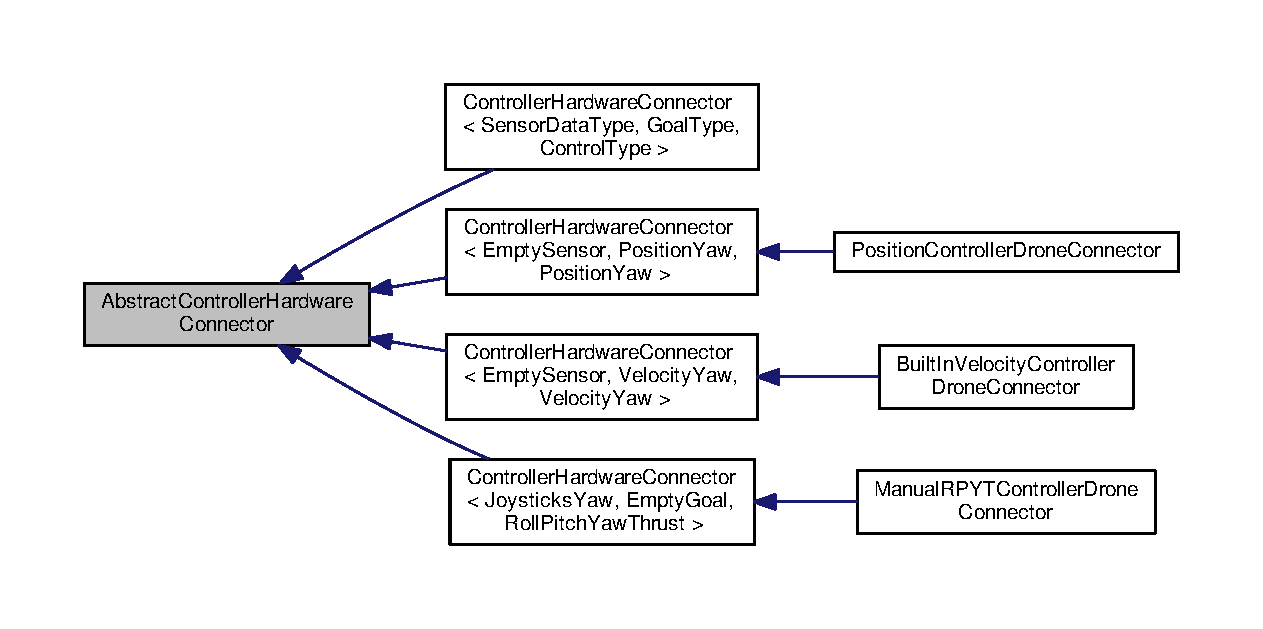
\includegraphics[width=350pt]{structAbstractControllerHardwareConnector__inherit__graph}
\end{center}
\end{figure}
\subsection*{Public Member Functions}
\begin{DoxyCompactItemize}
\item 
virtual void \hyperlink{structAbstractControllerHardwareConnector_a0fcf605e19daef2f9f99d4dc2a23feb4}{run} ()=0
\begin{DoxyCompactList}\small\item\em Abstract run function. \end{DoxyCompactList}\item 
virtual \hyperlink{structAbstractControllerHardwareConnector_a06f931d74faac604c3ef56cb5ba75399}{$\sim$\-Abstract\-Controller\-Hardware\-Connector} ()
\begin{DoxyCompactList}\small\item\em Destructor to get polymorphism. \end{DoxyCompactList}\end{DoxyCompactItemize}


\subsection{Detailed Description}
Base for \hyperlink{classControllerHardwareConnector}{Controller\-Hardware\-Connector} class. 

\subsection{Constructor \& Destructor Documentation}
\hypertarget{structAbstractControllerHardwareConnector_a06f931d74faac604c3ef56cb5ba75399}{\index{Abstract\-Controller\-Hardware\-Connector@{Abstract\-Controller\-Hardware\-Connector}!$\sim$\-Abstract\-Controller\-Hardware\-Connector@{$\sim$\-Abstract\-Controller\-Hardware\-Connector}}
\index{$\sim$\-Abstract\-Controller\-Hardware\-Connector@{$\sim$\-Abstract\-Controller\-Hardware\-Connector}!AbstractControllerHardwareConnector@{Abstract\-Controller\-Hardware\-Connector}}
\subsubsection[{$\sim$\-Abstract\-Controller\-Hardware\-Connector}]{\setlength{\rightskip}{0pt plus 5cm}virtual Abstract\-Controller\-Hardware\-Connector\-::$\sim$\-Abstract\-Controller\-Hardware\-Connector (
\begin{DoxyParamCaption}
{}
\end{DoxyParamCaption}
)\hspace{0.3cm}{\ttfamily [inline]}, {\ttfamily [virtual]}}}\label{structAbstractControllerHardwareConnector_a06f931d74faac604c3ef56cb5ba75399}


Destructor to get polymorphism. 



\subsection{Member Function Documentation}
\hypertarget{structAbstractControllerHardwareConnector_a0fcf605e19daef2f9f99d4dc2a23feb4}{\index{Abstract\-Controller\-Hardware\-Connector@{Abstract\-Controller\-Hardware\-Connector}!run@{run}}
\index{run@{run}!AbstractControllerHardwareConnector@{Abstract\-Controller\-Hardware\-Connector}}
\subsubsection[{run}]{\setlength{\rightskip}{0pt plus 5cm}virtual void Abstract\-Controller\-Hardware\-Connector\-::run (
\begin{DoxyParamCaption}
{}
\end{DoxyParamCaption}
)\hspace{0.3cm}{\ttfamily [pure virtual]}}}\label{structAbstractControllerHardwareConnector_a0fcf605e19daef2f9f99d4dc2a23feb4}


Abstract run function. 

The run function should run controller and send commands to hardware 

Implemented in \hyperlink{classControllerHardwareConnector_afb46464434a3a5881ecc1091f58bbd61}{Controller\-Hardware\-Connector$<$ Sensor\-Data\-Type, Goal\-Type, Control\-Type $>$}, \hyperlink{classControllerHardwareConnector_afb46464434a3a5881ecc1091f58bbd61}{Controller\-Hardware\-Connector$<$ Joysticks\-Yaw, Empty\-Goal, Roll\-Pitch\-Yaw\-Thrust $>$}, \hyperlink{classControllerHardwareConnector_afb46464434a3a5881ecc1091f58bbd61}{Controller\-Hardware\-Connector$<$ Empty\-Sensor, Velocity\-Yaw, Velocity\-Yaw $>$}, and \hyperlink{classControllerHardwareConnector_afb46464434a3a5881ecc1091f58bbd61}{Controller\-Hardware\-Connector$<$ Empty\-Sensor, Position\-Yaw, Position\-Yaw $>$}.



The documentation for this struct was generated from the following file\-:\begin{DoxyCompactItemize}
\item 
include/aerial\-\_\-autonomy/controller\-\_\-hardware\-\_\-connectors/\hyperlink{base__controller__hardware__connector_8h}{base\-\_\-controller\-\_\-hardware\-\_\-connector.\-h}\end{DoxyCompactItemize}

\hypertarget{structActionFunctor}{\section{Action\-Functor$<$ Event\-T, Robot\-System\-T, Logic\-State\-Machine\-T $>$ Struct Template Reference}
\label{structActionFunctor}\index{Action\-Functor$<$ Event\-T, Robot\-System\-T, Logic\-State\-Machine\-T $>$@{Action\-Functor$<$ Event\-T, Robot\-System\-T, Logic\-State\-Machine\-T $>$}}
}


Action Functor for a given event, robot system, state machine.  




{\ttfamily \#include $<$base\-\_\-functors.\-h$>$}

\subsection*{Public Member Functions}
\begin{DoxyCompactItemize}
\item 
virtual void \hyperlink{structActionFunctor_a97250a2cc027dc3ca7d10a975d11a5c7}{run} (Event\-T const \&event, Robot\-System\-T \&robot\-\_\-system, Logic\-State\-Machine\-T \&logic\-\_\-state\-\_\-machine)=0
\begin{DoxyCompactList}\small\item\em Override this run function for different sub classes. This function performs the logic checking for each state. \end{DoxyCompactList}\item 
{\footnotesize template$<$class F\-S\-M , class Source\-State , class Target\-State $>$ }\\void \hyperlink{structActionFunctor_adbf24aea135ecf5a0d470b290a5cab02}{operator()} (Event\-T const \&event, F\-S\-M \&logic\-\_\-state\-\_\-machine, Source\-State \&, Target\-State \&)
\begin{DoxyCompactList}\small\item\em operator () Internally calls run function \end{DoxyCompactList}\item 
virtual \hyperlink{structActionFunctor_aaaa4c1ce7204b370be55f2ef4a618258}{$\sim$\-Action\-Functor} ()
\begin{DoxyCompactList}\small\item\em Virtual destructor to obtain polymorphism. \end{DoxyCompactList}\end{DoxyCompactItemize}


\subsection{Detailed Description}
\subsubsection*{template$<$class Event\-T, class Robot\-System\-T, class Logic\-State\-Machine\-T$>$struct Action\-Functor$<$ Event\-T, Robot\-System\-T, Logic\-State\-Machine\-T $>$}

Action Functor for a given event, robot system, state machine. 

This class provides run function for state transitions Derived states have to implement the specific run function behavior using this base class.


\begin{DoxyTemplParams}{Template Parameters}
{\em Event\-T} & Event triggering this action \\
\hline
{\em Robot\-System\-T} & The robot system used in the action \\
\hline
{\em Logic\-State\-Machine\-T} & The logic state machine used to trigger events \\
\hline
\end{DoxyTemplParams}


\subsection{Constructor \& Destructor Documentation}
\hypertarget{structActionFunctor_aaaa4c1ce7204b370be55f2ef4a618258}{\index{Action\-Functor@{Action\-Functor}!$\sim$\-Action\-Functor@{$\sim$\-Action\-Functor}}
\index{$\sim$\-Action\-Functor@{$\sim$\-Action\-Functor}!ActionFunctor@{Action\-Functor}}
\subsubsection[{$\sim$\-Action\-Functor}]{\setlength{\rightskip}{0pt plus 5cm}template$<$class Event\-T, class Robot\-System\-T, class Logic\-State\-Machine\-T$>$ virtual {\bf Action\-Functor}$<$ Event\-T, Robot\-System\-T, Logic\-State\-Machine\-T $>$\-::$\sim${\bf Action\-Functor} (
\begin{DoxyParamCaption}
{}
\end{DoxyParamCaption}
)\hspace{0.3cm}{\ttfamily [inline]}, {\ttfamily [virtual]}}}\label{structActionFunctor_aaaa4c1ce7204b370be55f2ef4a618258}


Virtual destructor to obtain polymorphism. 



\subsection{Member Function Documentation}
\hypertarget{structActionFunctor_adbf24aea135ecf5a0d470b290a5cab02}{\index{Action\-Functor@{Action\-Functor}!operator()@{operator()}}
\index{operator()@{operator()}!ActionFunctor@{Action\-Functor}}
\subsubsection[{operator()}]{\setlength{\rightskip}{0pt plus 5cm}template$<$class Event\-T, class Robot\-System\-T, class Logic\-State\-Machine\-T$>$ template$<$class F\-S\-M , class Source\-State , class Target\-State $>$ void {\bf Action\-Functor}$<$ Event\-T, Robot\-System\-T, Logic\-State\-Machine\-T $>$\-::operator() (
\begin{DoxyParamCaption}
\item[{Event\-T const \&}]{event, }
\item[{F\-S\-M \&}]{logic\-\_\-state\-\_\-machine, }
\item[{Source\-State \&}]{, }
\item[{Target\-State \&}]{}
\end{DoxyParamCaption}
)\hspace{0.3cm}{\ttfamily [inline]}}}\label{structActionFunctor_adbf24aea135ecf5a0d470b290a5cab02}


operator () Internally calls run function 


\begin{DoxyParams}{Parameters}
{\em logic\-\_\-state\-\_\-machine} & Backend of logic State Machine. can send events using this. \\
\hline
{\em event} & Event triggering the action \\
\hline
\end{DoxyParams}
\hypertarget{structActionFunctor_a97250a2cc027dc3ca7d10a975d11a5c7}{\index{Action\-Functor@{Action\-Functor}!run@{run}}
\index{run@{run}!ActionFunctor@{Action\-Functor}}
\subsubsection[{run}]{\setlength{\rightskip}{0pt plus 5cm}template$<$class Event\-T, class Robot\-System\-T, class Logic\-State\-Machine\-T$>$ virtual void {\bf Action\-Functor}$<$ Event\-T, Robot\-System\-T, Logic\-State\-Machine\-T $>$\-::run (
\begin{DoxyParamCaption}
\item[{Event\-T const \&}]{event, }
\item[{Robot\-System\-T \&}]{robot\-\_\-system, }
\item[{Logic\-State\-Machine\-T \&}]{logic\-\_\-state\-\_\-machine}
\end{DoxyParamCaption}
)\hspace{0.3cm}{\ttfamily [pure virtual]}}}\label{structActionFunctor_a97250a2cc027dc3ca7d10a975d11a5c7}


Override this run function for different sub classes. This function performs the logic checking for each state. 


\begin{DoxyParams}{Parameters}
{\em robot\-\_\-system} & Provides sensor data and allows for controlling hardware \\
\hline
{\em logic\-\_\-state\-\_\-machine} & Backend of logic State Machine. can send events using this. \\
\hline
{\em event} & Event triggering the action \\
\hline
\end{DoxyParams}


Implemented in \hyperlink{structPositionControlTransitionActionFunctor___a4970bb461809ffa30984e16902bb8aaa}{Position\-Control\-Transition\-Action\-Functor\-\_\-$<$ Logic\-State\-Machine\-T $>$}.



The documentation for this struct was generated from the following file\-:\begin{DoxyCompactItemize}
\item 
include/aerial\-\_\-autonomy/actions\-\_\-guards/\hyperlink{base__functors_8h}{base\-\_\-functors.\-h}\end{DoxyCompactItemize}

\hypertarget{classAsyncTimer}{\section{Async\-Timer Class Reference}
\label{classAsyncTimer}\index{Async\-Timer@{Async\-Timer}}
}


Calls given function on a timer in its own thread.  




{\ttfamily \#include $<$async\-\_\-timer.\-h$>$}

\subsection*{Public Member Functions}
\begin{DoxyCompactItemize}
\item 
\hyperlink{classAsyncTimer_a8509db3cc448bd8f313435150baf434d}{Async\-Timer} (std\-::function$<$ void()$>$ function, std\-::chrono\-::duration$<$ double $>$ timer\-\_\-duration)
\begin{DoxyCompactList}\small\item\em Constructor. \end{DoxyCompactList}\item 
virtual \hyperlink{classAsyncTimer_a92781264c62bcbad0b9ffd447d0cb3fd}{$\sim$\-Async\-Timer} ()
\begin{DoxyCompactList}\small\item\em Destructor cleans up running thread. \end{DoxyCompactList}\item 
void \hyperlink{classAsyncTimer_ab058544794ccb0310eb5a803458de860}{start} ()
\begin{DoxyCompactList}\small\item\em Starts running the timer thread. \end{DoxyCompactList}\end{DoxyCompactItemize}


\subsection{Detailed Description}
Calls given function on a timer in its own thread. 

\subsection{Constructor \& Destructor Documentation}
\hypertarget{classAsyncTimer_a8509db3cc448bd8f313435150baf434d}{\index{Async\-Timer@{Async\-Timer}!Async\-Timer@{Async\-Timer}}
\index{Async\-Timer@{Async\-Timer}!AsyncTimer@{Async\-Timer}}
\subsubsection[{Async\-Timer}]{\setlength{\rightskip}{0pt plus 5cm}Async\-Timer\-::\-Async\-Timer (
\begin{DoxyParamCaption}
\item[{std\-::function$<$ void()$>$}]{function, }
\item[{std\-::chrono\-::duration$<$ double $>$}]{timer\-\_\-duration}
\end{DoxyParamCaption}
)}}\label{classAsyncTimer_a8509db3cc448bd8f313435150baf434d}


Constructor. 


\begin{DoxyParams}{Parameters}
{\em function} & Function to call \\
\hline
{\em timer\-\_\-duration} & The amount of time in between each function call \\
\hline
\end{DoxyParams}
\hypertarget{classAsyncTimer_a92781264c62bcbad0b9ffd447d0cb3fd}{\index{Async\-Timer@{Async\-Timer}!$\sim$\-Async\-Timer@{$\sim$\-Async\-Timer}}
\index{$\sim$\-Async\-Timer@{$\sim$\-Async\-Timer}!AsyncTimer@{Async\-Timer}}
\subsubsection[{$\sim$\-Async\-Timer}]{\setlength{\rightskip}{0pt plus 5cm}Async\-Timer\-::$\sim$\-Async\-Timer (
\begin{DoxyParamCaption}
{}
\end{DoxyParamCaption}
)\hspace{0.3cm}{\ttfamily [virtual]}}}\label{classAsyncTimer_a92781264c62bcbad0b9ffd447d0cb3fd}


Destructor cleans up running thread. 



\subsection{Member Function Documentation}
\hypertarget{classAsyncTimer_ab058544794ccb0310eb5a803458de860}{\index{Async\-Timer@{Async\-Timer}!start@{start}}
\index{start@{start}!AsyncTimer@{Async\-Timer}}
\subsubsection[{start}]{\setlength{\rightskip}{0pt plus 5cm}void Async\-Timer\-::start (
\begin{DoxyParamCaption}
{}
\end{DoxyParamCaption}
)}}\label{classAsyncTimer_ab058544794ccb0310eb5a803458de860}


Starts running the timer thread. 



The documentation for this class was generated from the following files\-:\begin{DoxyCompactItemize}
\item 
include/aerial\-\_\-autonomy/common/\hyperlink{async__timer_8h}{async\-\_\-timer.\-h}\item 
src/common/\hyperlink{async__timer_8cpp}{async\-\_\-timer.\-cpp}\end{DoxyCompactItemize}

\hypertarget{classBaseState}{\section{Base\-State$<$ Robot\-System\-T, Logic\-State\-Machine\-T, Action\-Fctr $>$ Class Template Reference}
\label{classBaseState}\index{Base\-State$<$ Robot\-System\-T, Logic\-State\-Machine\-T, Action\-Fctr $>$@{Base\-State$<$ Robot\-System\-T, Logic\-State\-Machine\-T, Action\-Fctr $>$}}
}


Base state for all states in logic state machine.  




{\ttfamily \#include $<$base\-\_\-state.\-h$>$}



Inheritance diagram for Base\-State$<$ Robot\-System\-T, Logic\-State\-Machine\-T, Action\-Fctr $>$\-:\nopagebreak
\begin{figure}[H]
\begin{center}
\leavevmode
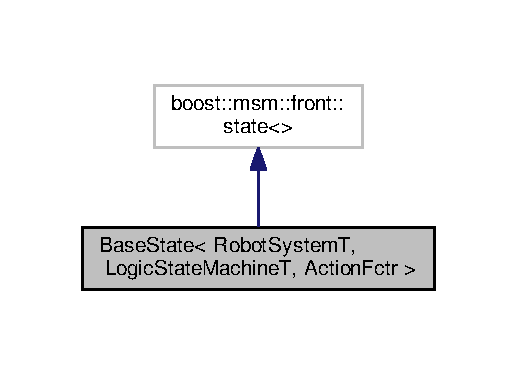
\includegraphics[width=248pt]{classBaseState__inherit__graph}
\end{center}
\end{figure}


Collaboration diagram for Base\-State$<$ Robot\-System\-T, Logic\-State\-Machine\-T, Action\-Fctr $>$\-:\nopagebreak
\begin{figure}[H]
\begin{center}
\leavevmode
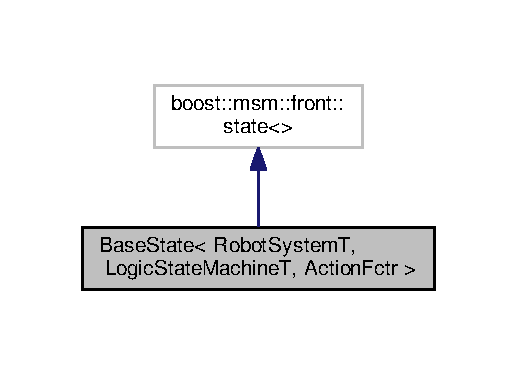
\includegraphics[width=248pt]{classBaseState__coll__graph}
\end{center}
\end{figure}
\subsection*{Classes}
\begin{DoxyCompactItemize}
\item 
struct \hyperlink{structBaseState_1_1internal__transition__table}{internal\-\_\-transition\-\_\-table}
\begin{DoxyCompactList}\small\item\em The \hyperlink{structBaseState_1_1internal__transition__table}{internal\-\_\-transition\-\_\-table} to call run function in every state. \end{DoxyCompactList}\end{DoxyCompactItemize}
\subsection*{Public Member Functions}
\begin{DoxyCompactItemize}
\item 
virtual \hyperlink{classBaseState_a3967d85ffd88b9235fcfd9732e745c13}{$\sim$\-Base\-State} ()
\begin{DoxyCompactList}\small\item\em Destructor. \end{DoxyCompactList}\end{DoxyCompactItemize}


\subsection{Detailed Description}
\subsubsection*{template$<$class Robot\-System\-T, class Logic\-State\-Machine\-T, class Action\-Fctr$>$class Base\-State$<$ Robot\-System\-T, Logic\-State\-Machine\-T, Action\-Fctr $>$}

Base state for all states in logic state machine. 

This class provides a wrapper for any action function and robot system Entry and exit function can also be overwritten by subclassing this base state. 

\subsection{Constructor \& Destructor Documentation}
\hypertarget{classBaseState_a3967d85ffd88b9235fcfd9732e745c13}{\index{Base\-State@{Base\-State}!$\sim$\-Base\-State@{$\sim$\-Base\-State}}
\index{$\sim$\-Base\-State@{$\sim$\-Base\-State}!BaseState@{Base\-State}}
\subsubsection[{$\sim$\-Base\-State}]{\setlength{\rightskip}{0pt plus 5cm}template$<$class Robot\-System\-T , class Logic\-State\-Machine\-T , class Action\-Fctr $>$ virtual {\bf Base\-State}$<$ Robot\-System\-T, Logic\-State\-Machine\-T, Action\-Fctr $>$\-::$\sim${\bf Base\-State} (
\begin{DoxyParamCaption}
{}
\end{DoxyParamCaption}
)\hspace{0.3cm}{\ttfamily [inline]}, {\ttfamily [virtual]}}}\label{classBaseState_a3967d85ffd88b9235fcfd9732e745c13}


Destructor. 



The documentation for this class was generated from the following file\-:\begin{DoxyCompactItemize}
\item 
include/aerial\-\_\-autonomy/logic\-\_\-states/\hyperlink{base__state_8h}{base\-\_\-state.\-h}\end{DoxyCompactItemize}

\hypertarget{classBuiltInController}{\section{Built\-In\-Controller$<$ Goal\-Type $>$ Class Template Reference}
\label{classBuiltInController}\index{Built\-In\-Controller$<$ Goal\-Type $>$@{Built\-In\-Controller$<$ Goal\-Type $>$}}
}


A controller that simply outputs the set goal.  




{\ttfamily \#include $<$builtin\-\_\-controller.\-h$>$}



Inheritance diagram for Built\-In\-Controller$<$ Goal\-Type $>$\-:\nopagebreak
\begin{figure}[H]
\begin{center}
\leavevmode
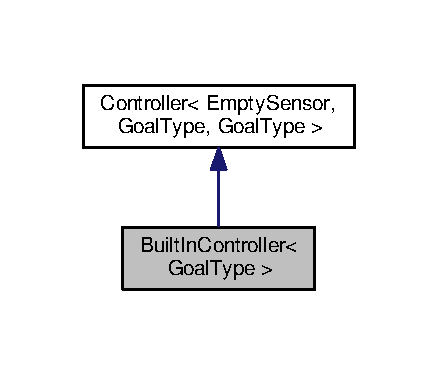
\includegraphics[width=210pt]{classBuiltInController__inherit__graph}
\end{center}
\end{figure}


Collaboration diagram for Built\-In\-Controller$<$ Goal\-Type $>$\-:\nopagebreak
\begin{figure}[H]
\begin{center}
\leavevmode
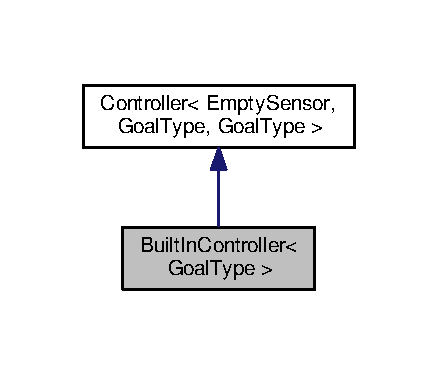
\includegraphics[width=210pt]{classBuiltInController__coll__graph}
\end{center}
\end{figure}
\subsection*{Public Member Functions}
\begin{DoxyCompactItemize}
\item 
virtual \hyperlink{classBuiltInController_aea6ab422dc24222fb168a7e9522ec7c9}{$\sim$\-Built\-In\-Controller} ()
\begin{DoxyCompactList}\small\item\em Destructor. \end{DoxyCompactList}\end{DoxyCompactItemize}
\subsection*{Protected Member Functions}
\begin{DoxyCompactItemize}
\item 
virtual Goal\-Type \hyperlink{classBuiltInController_ab597ac5aa54f9865c0324fbcf5c0d7bd}{run\-Implementation} (\hyperlink{structEmptySensor}{Empty\-Sensor} sensor\-\_\-data, Goal\-Type goal)
\begin{DoxyCompactList}\small\item\em Run the control loop. Simply returns the goal. \end{DoxyCompactList}\end{DoxyCompactItemize}


\subsection{Detailed Description}
\subsubsection*{template$<$class Goal\-Type$>$class Built\-In\-Controller$<$ Goal\-Type $>$}

A controller that simply outputs the set goal. 

\subsection{Constructor \& Destructor Documentation}
\hypertarget{classBuiltInController_aea6ab422dc24222fb168a7e9522ec7c9}{\index{Built\-In\-Controller@{Built\-In\-Controller}!$\sim$\-Built\-In\-Controller@{$\sim$\-Built\-In\-Controller}}
\index{$\sim$\-Built\-In\-Controller@{$\sim$\-Built\-In\-Controller}!BuiltInController@{Built\-In\-Controller}}
\subsubsection[{$\sim$\-Built\-In\-Controller}]{\setlength{\rightskip}{0pt plus 5cm}template$<$class Goal\-Type$>$ virtual {\bf Built\-In\-Controller}$<$ Goal\-Type $>$\-::$\sim${\bf Built\-In\-Controller} (
\begin{DoxyParamCaption}
{}
\end{DoxyParamCaption}
)\hspace{0.3cm}{\ttfamily [inline]}, {\ttfamily [virtual]}}}\label{classBuiltInController_aea6ab422dc24222fb168a7e9522ec7c9}


Destructor. 



\subsection{Member Function Documentation}
\hypertarget{classBuiltInController_ab597ac5aa54f9865c0324fbcf5c0d7bd}{\index{Built\-In\-Controller@{Built\-In\-Controller}!run\-Implementation@{run\-Implementation}}
\index{run\-Implementation@{run\-Implementation}!BuiltInController@{Built\-In\-Controller}}
\subsubsection[{run\-Implementation}]{\setlength{\rightskip}{0pt plus 5cm}template$<$class Goal\-Type$>$ virtual Goal\-Type {\bf Built\-In\-Controller}$<$ Goal\-Type $>$\-::run\-Implementation (
\begin{DoxyParamCaption}
\item[{{\bf Empty\-Sensor}}]{sensor\-\_\-data, }
\item[{Goal\-Type}]{goal}
\end{DoxyParamCaption}
)\hspace{0.3cm}{\ttfamily [inline]}, {\ttfamily [protected]}, {\ttfamily [virtual]}}}\label{classBuiltInController_ab597ac5aa54f9865c0324fbcf5c0d7bd}


Run the control loop. Simply returns the goal. 


\begin{DoxyParams}{Parameters}
{\em sensor\-\_\-data} & Empty sensor data struct since no sensing is required. \\
\hline
{\em goal} & Goal set-\/point \\
\hline
\end{DoxyParams}
\begin{DoxyReturn}{Returns}
Goal to send to hardware 
\end{DoxyReturn}


Implements \hyperlink{classController_a9a5a0b6fbedeb476f3a7bfad5f16167e}{Controller$<$ Empty\-Sensor, Goal\-Type, Goal\-Type $>$}.



The documentation for this class was generated from the following file\-:\begin{DoxyCompactItemize}
\item 
include/aerial\-\_\-autonomy/controllers/\hyperlink{builtin__controller_8h}{builtin\-\_\-controller.\-h}\end{DoxyCompactItemize}

\hypertarget{classBuiltInVelocityControllerDroneConnector}{\section{Built\-In\-Velocity\-Controller\-Drone\-Connector Class Reference}
\label{classBuiltInVelocityControllerDroneConnector}\index{Built\-In\-Velocity\-Controller\-Drone\-Connector@{Built\-In\-Velocity\-Controller\-Drone\-Connector}}
}


Manages communication between a drone plugin and a velocity controller that outputs velocity commands.  




{\ttfamily \#include $<$builtin\-\_\-velocity\-\_\-controller\-\_\-drone\-\_\-connector.\-h$>$}



Inheritance diagram for Built\-In\-Velocity\-Controller\-Drone\-Connector\-:\nopagebreak
\begin{figure}[H]
\begin{center}
\leavevmode
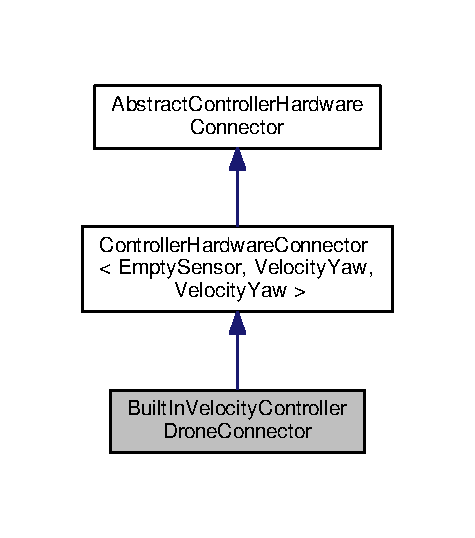
\includegraphics[width=228pt]{classBuiltInVelocityControllerDroneConnector__inherit__graph}
\end{center}
\end{figure}


Collaboration diagram for Built\-In\-Velocity\-Controller\-Drone\-Connector\-:\nopagebreak
\begin{figure}[H]
\begin{center}
\leavevmode
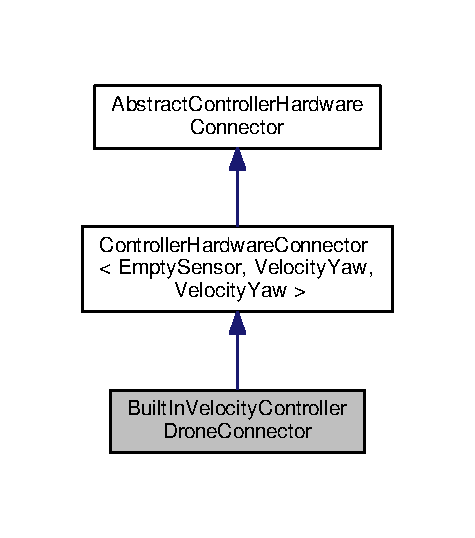
\includegraphics[width=228pt]{classBuiltInVelocityControllerDroneConnector__coll__graph}
\end{center}
\end{figure}
\subsection*{Public Member Functions}
\begin{DoxyCompactItemize}
\item 
\hyperlink{classBuiltInVelocityControllerDroneConnector_a2a9693047db6fcdadea21d54bfe10fc1}{Built\-In\-Velocity\-Controller\-Drone\-Connector} (parsernode\-::\-Parser \&drone\-\_\-hardware, \hyperlink{classController}{Controller}$<$ \hyperlink{structEmptySensor}{Empty\-Sensor}, \hyperlink{structVelocityYaw}{Velocity\-Yaw}, \hyperlink{structVelocityYaw}{Velocity\-Yaw} $>$ \&controller)
\begin{DoxyCompactList}\small\item\em Constructor. \end{DoxyCompactList}\end{DoxyCompactItemize}
\subsection*{Protected Member Functions}
\begin{DoxyCompactItemize}
\item 
virtual \hyperlink{structEmptySensor}{Empty\-Sensor} \hyperlink{classBuiltInVelocityControllerDroneConnector_af69ba169f039d9f8d59f675392af4cf0}{extract\-Sensor\-Data} ()
\begin{DoxyCompactList}\small\item\em does not extract any data since nothing is needed \end{DoxyCompactList}\item 
virtual void \hyperlink{classBuiltInVelocityControllerDroneConnector_a10a06a14a9a34afbe37c79e86ffd5787}{send\-Hardware\-Commands} (\hyperlink{structVelocityYaw}{Velocity\-Yaw} controls)
\begin{DoxyCompactList}\small\item\em Send velocity commands to hardware. \end{DoxyCompactList}\end{DoxyCompactItemize}
\subsection*{Additional Inherited Members}


\subsection{Detailed Description}
Manages communication between a drone plugin and a velocity controller that outputs velocity commands. 

\subsection{Constructor \& Destructor Documentation}
\hypertarget{classBuiltInVelocityControllerDroneConnector_a2a9693047db6fcdadea21d54bfe10fc1}{\index{Built\-In\-Velocity\-Controller\-Drone\-Connector@{Built\-In\-Velocity\-Controller\-Drone\-Connector}!Built\-In\-Velocity\-Controller\-Drone\-Connector@{Built\-In\-Velocity\-Controller\-Drone\-Connector}}
\index{Built\-In\-Velocity\-Controller\-Drone\-Connector@{Built\-In\-Velocity\-Controller\-Drone\-Connector}!BuiltInVelocityControllerDroneConnector@{Built\-In\-Velocity\-Controller\-Drone\-Connector}}
\subsubsection[{Built\-In\-Velocity\-Controller\-Drone\-Connector}]{\setlength{\rightskip}{0pt plus 5cm}Built\-In\-Velocity\-Controller\-Drone\-Connector\-::\-Built\-In\-Velocity\-Controller\-Drone\-Connector (
\begin{DoxyParamCaption}
\item[{parsernode\-::\-Parser \&}]{drone\-\_\-hardware, }
\item[{{\bf Controller}$<$ {\bf Empty\-Sensor}, {\bf Velocity\-Yaw}, {\bf Velocity\-Yaw} $>$ \&}]{controller}
\end{DoxyParamCaption}
)\hspace{0.3cm}{\ttfamily [inline]}}}\label{classBuiltInVelocityControllerDroneConnector_a2a9693047db6fcdadea21d54bfe10fc1}


Constructor. 

Store drone hardware with hardware type as U\-A\-V. Uses parsernode\-::\-Parser\-::cmdvelguided function.


\begin{DoxyParams}{Parameters}
{\em drone\-\_\-hardware} & Drone hardware used to send commands \\
\hline
{\em controller} & \hyperlink{structVelocity}{Velocity} controller that achieves a desired velocity, yaw \\
\hline
\end{DoxyParams}


\subsection{Member Function Documentation}
\hypertarget{classBuiltInVelocityControllerDroneConnector_af69ba169f039d9f8d59f675392af4cf0}{\index{Built\-In\-Velocity\-Controller\-Drone\-Connector@{Built\-In\-Velocity\-Controller\-Drone\-Connector}!extract\-Sensor\-Data@{extract\-Sensor\-Data}}
\index{extract\-Sensor\-Data@{extract\-Sensor\-Data}!BuiltInVelocityControllerDroneConnector@{Built\-In\-Velocity\-Controller\-Drone\-Connector}}
\subsubsection[{extract\-Sensor\-Data}]{\setlength{\rightskip}{0pt plus 5cm}{\bf Empty\-Sensor} Built\-In\-Velocity\-Controller\-Drone\-Connector\-::extract\-Sensor\-Data (
\begin{DoxyParamCaption}
{}
\end{DoxyParamCaption}
)\hspace{0.3cm}{\ttfamily [protected]}, {\ttfamily [virtual]}}}\label{classBuiltInVelocityControllerDroneConnector_af69ba169f039d9f8d59f675392af4cf0}


does not extract any data since nothing is needed 

\begin{DoxyReturn}{Returns}
empty data structure 
\end{DoxyReturn}


Implements \hyperlink{classControllerHardwareConnector_af6952c0d8829b93557eb7d8887bebd63}{Controller\-Hardware\-Connector$<$ Empty\-Sensor, Velocity\-Yaw, Velocity\-Yaw $>$}.

\hypertarget{classBuiltInVelocityControllerDroneConnector_a10a06a14a9a34afbe37c79e86ffd5787}{\index{Built\-In\-Velocity\-Controller\-Drone\-Connector@{Built\-In\-Velocity\-Controller\-Drone\-Connector}!send\-Hardware\-Commands@{send\-Hardware\-Commands}}
\index{send\-Hardware\-Commands@{send\-Hardware\-Commands}!BuiltInVelocityControllerDroneConnector@{Built\-In\-Velocity\-Controller\-Drone\-Connector}}
\subsubsection[{send\-Hardware\-Commands}]{\setlength{\rightskip}{0pt plus 5cm}void Built\-In\-Velocity\-Controller\-Drone\-Connector\-::send\-Hardware\-Commands (
\begin{DoxyParamCaption}
\item[{{\bf Velocity\-Yaw}}]{controls}
\end{DoxyParamCaption}
)\hspace{0.3cm}{\ttfamily [protected]}, {\ttfamily [virtual]}}}\label{classBuiltInVelocityControllerDroneConnector_a10a06a14a9a34afbe37c79e86ffd5787}


Send velocity commands to hardware. 


\begin{DoxyParams}{Parameters}
{\em controls} & velocity command to send to U\-A\-V \\
\hline
\end{DoxyParams}


Implements \hyperlink{classControllerHardwareConnector_a5fc86156d5c747aba36497732962d6d0}{Controller\-Hardware\-Connector$<$ Empty\-Sensor, Velocity\-Yaw, Velocity\-Yaw $>$}.



The documentation for this class was generated from the following files\-:\begin{DoxyCompactItemize}
\item 
include/aerial\-\_\-autonomy/controller\-\_\-hardware\-\_\-connectors/\hyperlink{builtin__velocity__controller__drone__connector_8h}{builtin\-\_\-velocity\-\_\-controller\-\_\-drone\-\_\-connector.\-h}\item 
src/controller\-\_\-hardware\-\_\-connectors/\hyperlink{builtin__velocity__controller__drone__connector_8cpp}{builtin\-\_\-velocity\-\_\-controller\-\_\-drone\-\_\-connector.\-cpp}\end{DoxyCompactItemize}

\hypertarget{structCompleted}{\section{Completed Struct Reference}
\label{structCompleted}\index{Completed@{Completed}}
}


\hyperlink{structCompleted}{Completed} Event for transition from for example Landing to Landed etc.  




{\ttfamily \#include $<$completed\-\_\-event.\-h$>$}



\subsection{Detailed Description}
\hyperlink{structCompleted}{Completed} Event for transition from for example Landing to Landed etc. 

The documentation for this struct was generated from the following file\-:\begin{DoxyCompactItemize}
\item 
include/aerial\-\_\-autonomy/types/\hyperlink{completed__event_8h}{completed\-\_\-event.\-h}\end{DoxyCompactItemize}

\hypertarget{classController}{\section{Controller$<$ Sensor\-Data\-Type, Goal\-Type, Control\-Type $>$ Class Template Reference}
\label{classController}\index{Controller$<$ Sensor\-Data\-Type, Goal\-Type, Control\-Type $>$@{Controller$<$ Sensor\-Data\-Type, Goal\-Type, Control\-Type $>$}}
}


Base \hyperlink{classController}{Controller} class.  




{\ttfamily \#include $<$base\-\_\-controller.\-h$>$}

\subsection*{Public Member Functions}
\begin{DoxyCompactItemize}
\item 
virtual Control\-Type \hyperlink{classController_a5caae261ff8a9f299cb8d220fbaf204b}{run} (Sensor\-Data\-Type sensor\-\_\-data)
\begin{DoxyCompactList}\small\item\em Run the control loop and return control arguments. \end{DoxyCompactList}\item 
virtual void \hyperlink{classController_a172aae7e2475b72fb2eb469ccd198387}{set\-Goal} (Goal\-Type goal)
\begin{DoxyCompactList}\small\item\em set the goal condition for the controller. Should use internal locking as the run function can be called from a separate thread \end{DoxyCompactList}\item 
virtual Goal\-Type \hyperlink{classController_a712cefd3af65956a9bd420641b175214}{get\-Goal} ()
\begin{DoxyCompactList}\small\item\em get the goal condition for the controller. Should use internal locking as the run function can be called from a separate thread \end{DoxyCompactList}\item 
virtual \hyperlink{classController_a86c5dbf78d3d948228c7c629e885151c}{$\sim$\-Controller} ()
\begin{DoxyCompactList}\small\item\em Destructor. \end{DoxyCompactList}\end{DoxyCompactItemize}
\subsection*{Protected Member Functions}
\begin{DoxyCompactItemize}
\item 
virtual Control\-Type \hyperlink{classController_a9a5a0b6fbedeb476f3a7bfad5f16167e}{run\-Implementation} (Sensor\-Data\-Type sensor\-\_\-data, Goal\-Type goal)=0
\begin{DoxyCompactList}\small\item\em Run the control loop and return control arguments. \end{DoxyCompactList}\end{DoxyCompactItemize}


\subsection{Detailed Description}
\subsubsection*{template$<$class Sensor\-Data\-Type, class Goal\-Type, class Control\-Type$>$class Controller$<$ Sensor\-Data\-Type, Goal\-Type, Control\-Type $>$}

Base \hyperlink{classController}{Controller} class. 

subclass should implement the run\-Implementation function which takes as input the sensor data and the desired goal and returns a control value.


\begin{DoxyTemplParams}{Template Parameters}
{\em Sensor\-Data\-Type} & The type of sensor the controller takes in \\
\hline
{\em Goal\-Type} & The type of goal the controller takes in \\
\hline
{\em Control\-Type} & The type of control the controller returns \\
\hline
\end{DoxyTemplParams}


\subsection{Constructor \& Destructor Documentation}
\hypertarget{classController_a86c5dbf78d3d948228c7c629e885151c}{\index{Controller@{Controller}!$\sim$\-Controller@{$\sim$\-Controller}}
\index{$\sim$\-Controller@{$\sim$\-Controller}!Controller@{Controller}}
\subsubsection[{$\sim$\-Controller}]{\setlength{\rightskip}{0pt plus 5cm}template$<$class Sensor\-Data\-Type, class Goal\-Type, class Control\-Type$>$ virtual {\bf Controller}$<$ Sensor\-Data\-Type, Goal\-Type, Control\-Type $>$\-::$\sim${\bf Controller} (
\begin{DoxyParamCaption}
{}
\end{DoxyParamCaption}
)\hspace{0.3cm}{\ttfamily [inline]}, {\ttfamily [virtual]}}}\label{classController_a86c5dbf78d3d948228c7c629e885151c}


Destructor. 



\subsection{Member Function Documentation}
\hypertarget{classController_a712cefd3af65956a9bd420641b175214}{\index{Controller@{Controller}!get\-Goal@{get\-Goal}}
\index{get\-Goal@{get\-Goal}!Controller@{Controller}}
\subsubsection[{get\-Goal}]{\setlength{\rightskip}{0pt plus 5cm}template$<$class Sensor\-Data\-Type, class Goal\-Type, class Control\-Type$>$ virtual Goal\-Type {\bf Controller}$<$ Sensor\-Data\-Type, Goal\-Type, Control\-Type $>$\-::get\-Goal (
\begin{DoxyParamCaption}
{}
\end{DoxyParamCaption}
)\hspace{0.3cm}{\ttfamily [inline]}, {\ttfamily [virtual]}}}\label{classController_a712cefd3af65956a9bd420641b175214}


get the goal condition for the controller. Should use internal locking as the run function can be called from a separate thread 

\hypertarget{classController_a5caae261ff8a9f299cb8d220fbaf204b}{\index{Controller@{Controller}!run@{run}}
\index{run@{run}!Controller@{Controller}}
\subsubsection[{run}]{\setlength{\rightskip}{0pt plus 5cm}template$<$class Sensor\-Data\-Type, class Goal\-Type, class Control\-Type$>$ virtual Control\-Type {\bf Controller}$<$ Sensor\-Data\-Type, Goal\-Type, Control\-Type $>$\-::run (
\begin{DoxyParamCaption}
\item[{Sensor\-Data\-Type}]{sensor\-\_\-data}
\end{DoxyParamCaption}
)\hspace{0.3cm}{\ttfamily [inline]}, {\ttfamily [virtual]}}}\label{classController_a5caae261ff8a9f299cb8d220fbaf204b}


Run the control loop and return control arguments. 


\begin{DoxyParams}{Parameters}
{\em sensor\-\_\-data} & Data required for control loop. Can also be estimator data \\
\hline
\end{DoxyParams}
\begin{DoxyReturn}{Returns}
Control values to send to hardware 
\end{DoxyReturn}
\hypertarget{classController_a9a5a0b6fbedeb476f3a7bfad5f16167e}{\index{Controller@{Controller}!run\-Implementation@{run\-Implementation}}
\index{run\-Implementation@{run\-Implementation}!Controller@{Controller}}
\subsubsection[{run\-Implementation}]{\setlength{\rightskip}{0pt plus 5cm}template$<$class Sensor\-Data\-Type, class Goal\-Type, class Control\-Type$>$ virtual Control\-Type {\bf Controller}$<$ Sensor\-Data\-Type, Goal\-Type, Control\-Type $>$\-::run\-Implementation (
\begin{DoxyParamCaption}
\item[{Sensor\-Data\-Type}]{sensor\-\_\-data, }
\item[{Goal\-Type}]{goal}
\end{DoxyParamCaption}
)\hspace{0.3cm}{\ttfamily [protected]}, {\ttfamily [pure virtual]}}}\label{classController_a9a5a0b6fbedeb476f3a7bfad5f16167e}


Run the control loop and return control arguments. 


\begin{DoxyParams}{Parameters}
{\em sensor\-\_\-data} & Data required for control loop. Can also be estimator data \\
\hline
{\em goal} & The set-\/point for the controller \\
\hline
\end{DoxyParams}
\begin{DoxyReturn}{Returns}
Control values to send to hardware 
\end{DoxyReturn}


Implemented in \hyperlink{classManualRPYTController_ae29c56af6d0bc913d357c7849201c8fb}{Manual\-R\-P\-Y\-T\-Controller}, \hyperlink{classBuiltInController_ab597ac5aa54f9865c0324fbcf5c0d7bd}{Built\-In\-Controller$<$ Goal\-Type $>$}, \hyperlink{classBuiltInController_ab597ac5aa54f9865c0324fbcf5c0d7bd}{Built\-In\-Controller$<$ Position\-Yaw $>$}, and \hyperlink{classBuiltInController_ab597ac5aa54f9865c0324fbcf5c0d7bd}{Built\-In\-Controller$<$ Velocity\-Yaw $>$}.

\hypertarget{classController_a172aae7e2475b72fb2eb469ccd198387}{\index{Controller@{Controller}!set\-Goal@{set\-Goal}}
\index{set\-Goal@{set\-Goal}!Controller@{Controller}}
\subsubsection[{set\-Goal}]{\setlength{\rightskip}{0pt plus 5cm}template$<$class Sensor\-Data\-Type, class Goal\-Type, class Control\-Type$>$ virtual void {\bf Controller}$<$ Sensor\-Data\-Type, Goal\-Type, Control\-Type $>$\-::set\-Goal (
\begin{DoxyParamCaption}
\item[{Goal\-Type}]{goal}
\end{DoxyParamCaption}
)\hspace{0.3cm}{\ttfamily [inline]}, {\ttfamily [virtual]}}}\label{classController_a172aae7e2475b72fb2eb469ccd198387}


set the goal condition for the controller. Should use internal locking as the run function can be called from a separate thread 


\begin{DoxyParams}{Parameters}
{\em goal} & The goal for control loop \\
\hline
\end{DoxyParams}


The documentation for this class was generated from the following file\-:\begin{DoxyCompactItemize}
\item 
include/aerial\-\_\-autonomy/controllers/\hyperlink{base__controller_8h}{base\-\_\-controller.\-h}\end{DoxyCompactItemize}

\hypertarget{classControllerHardwareConnector}{\section{Controller\-Hardware\-Connector$<$ Sensor\-Data\-Type, Goal\-Type, Control\-Type $>$ Class Template Reference}
\label{classControllerHardwareConnector}\index{Controller\-Hardware\-Connector$<$ Sensor\-Data\-Type, Goal\-Type, Control\-Type $>$@{Controller\-Hardware\-Connector$<$ Sensor\-Data\-Type, Goal\-Type, Control\-Type $>$}}
}


Performs a single step of extracting data, running controller and sending data back to hardware.  




{\ttfamily \#include $<$base\-\_\-controller\-\_\-hardware\-\_\-connector.\-h$>$}



Inheritance diagram for Controller\-Hardware\-Connector$<$ Sensor\-Data\-Type, Goal\-Type, Control\-Type $>$\-:\nopagebreak
\begin{figure}[H]
\begin{center}
\leavevmode
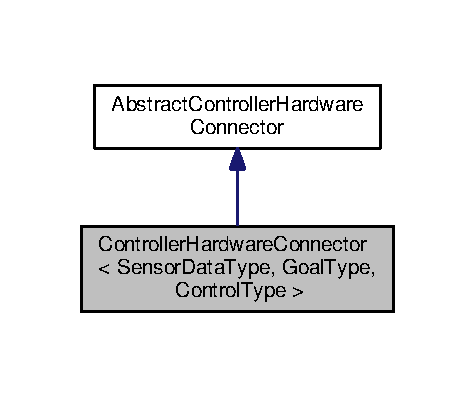
\includegraphics[width=228pt]{classControllerHardwareConnector__inherit__graph}
\end{center}
\end{figure}


Collaboration diagram for Controller\-Hardware\-Connector$<$ Sensor\-Data\-Type, Goal\-Type, Control\-Type $>$\-:\nopagebreak
\begin{figure}[H]
\begin{center}
\leavevmode
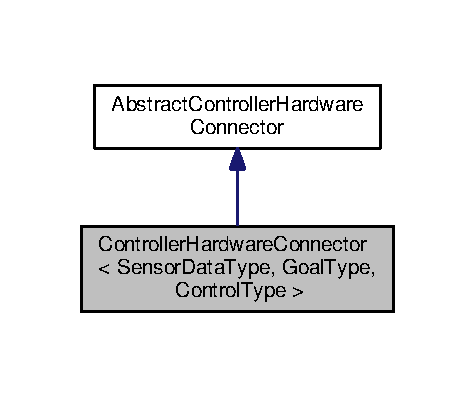
\includegraphics[width=228pt]{classControllerHardwareConnector__coll__graph}
\end{center}
\end{figure}
\subsection*{Public Member Functions}
\begin{DoxyCompactItemize}
\item 
\hyperlink{classControllerHardwareConnector_a6c5d8e5a5ded026ccee3d51f2899ce3e}{Controller\-Hardware\-Connector} (\hyperlink{classController}{Controller}$<$ Sensor\-Data\-Type, Goal\-Type, Control\-Type $>$ \&controller, \hyperlink{base__controller__hardware__connector_8h_ae4dfd42394001deb6e8a0e60c81d6f7a}{Hardware\-Type} hardware\-\_\-type)
\begin{DoxyCompactList}\small\item\em Control\-Hardware\-Connector runs the controller and sends the commands to hardware. \end{DoxyCompactList}\item 
virtual void \hyperlink{classControllerHardwareConnector_afb46464434a3a5881ecc1091f58bbd61}{run} ()
\begin{DoxyCompactList}\small\item\em Extracts sensor data, run controller and send data back to hardware. \end{DoxyCompactList}\item 
void \hyperlink{classControllerHardwareConnector_a14ce51377f80b67796fcb50ce8195efd}{set\-Goal} (Goal\-Type goal)
\begin{DoxyCompactList}\small\item\em Set the goal for controller. \end{DoxyCompactList}\item 
Goal\-Type \hyperlink{classControllerHardwareConnector_a1ea002003e277fc82e04615343b927f5}{get\-Goal} ()
\begin{DoxyCompactList}\small\item\em Get the goal for controller. \end{DoxyCompactList}\item 
\hyperlink{base__controller__hardware__connector_8h_ae4dfd42394001deb6e8a0e60c81d6f7a}{Hardware\-Type} \hyperlink{classControllerHardwareConnector_accd0c9bff560fa3c6d1e60d97644415e}{get\-Hardware\-Type} ()
\begin{DoxyCompactList}\small\item\em Return the type of hardware (Hardware\-Type) used by the controller. \end{DoxyCompactList}\end{DoxyCompactItemize}
\subsection*{Protected Member Functions}
\begin{DoxyCompactItemize}
\item 
virtual Sensor\-Data\-Type \hyperlink{classControllerHardwareConnector_af6952c0d8829b93557eb7d8887bebd63}{extract\-Sensor\-Data} ()=0
\begin{DoxyCompactList}\small\item\em extract relevant data from hardware/estimators \end{DoxyCompactList}\item 
virtual void \hyperlink{classControllerHardwareConnector_a5fc86156d5c747aba36497732962d6d0}{send\-Hardware\-Commands} (Control\-Type controls)=0
\begin{DoxyCompactList}\small\item\em Send hardware commands for example U\-A\-V rpy. \end{DoxyCompactList}\end{DoxyCompactItemize}
\subsection*{Protected Attributes}
\begin{DoxyCompactItemize}
\item 
\hyperlink{base__controller__hardware__connector_8h_ae4dfd42394001deb6e8a0e60c81d6f7a}{Hardware\-Type} \hyperlink{classControllerHardwareConnector_a1e47c12f796c9cc2fcb5c2495ede2392}{hardware\-\_\-type\-\_\-}
\begin{DoxyCompactList}\small\item\em Type of hardware controlled by the controller. \end{DoxyCompactList}\end{DoxyCompactItemize}


\subsection{Detailed Description}
\subsubsection*{template$<$class Sensor\-Data\-Type, class Goal\-Type, class Control\-Type$>$class Controller\-Hardware\-Connector$<$ Sensor\-Data\-Type, Goal\-Type, Control\-Type $>$}

Performs a single step of extracting data, running controller and sending data back to hardware. 


\begin{DoxyTemplParams}{Template Parameters}
{\em Sensor\-Data\-Type} & Type of data to take from hardware \\
\hline
{\em Goal\-Type} & Type of goal for controller \\
\hline
{\em Control\-Type} & Type of control sent to hardware \\
\hline
\end{DoxyTemplParams}


\subsection{Constructor \& Destructor Documentation}
\hypertarget{classControllerHardwareConnector_a6c5d8e5a5ded026ccee3d51f2899ce3e}{\index{Controller\-Hardware\-Connector@{Controller\-Hardware\-Connector}!Controller\-Hardware\-Connector@{Controller\-Hardware\-Connector}}
\index{Controller\-Hardware\-Connector@{Controller\-Hardware\-Connector}!ControllerHardwareConnector@{Controller\-Hardware\-Connector}}
\subsubsection[{Controller\-Hardware\-Connector}]{\setlength{\rightskip}{0pt plus 5cm}template$<$class Sensor\-Data\-Type, class Goal\-Type, class Control\-Type$>$ {\bf Controller\-Hardware\-Connector}$<$ Sensor\-Data\-Type, Goal\-Type, Control\-Type $>$\-::{\bf Controller\-Hardware\-Connector} (
\begin{DoxyParamCaption}
\item[{{\bf Controller}$<$ Sensor\-Data\-Type, Goal\-Type, Control\-Type $>$ \&}]{controller, }
\item[{{\bf Hardware\-Type}}]{hardware\-\_\-type}
\end{DoxyParamCaption}
)\hspace{0.3cm}{\ttfamily [inline]}}}\label{classControllerHardwareConnector_a6c5d8e5a5ded026ccee3d51f2899ce3e}


Control\-Hardware\-Connector runs the controller and sends the commands to hardware. 

The subclass controlhardwareconnectors should take the required hardware in the constructor and implement the run function to get the command from controller and send to hardware


\begin{DoxyParams}{Parameters}
{\em controller} & \hyperlink{classController}{Controller} to run during run function \\
\hline
{\em hardware\-\_\-type} & Type of Hardware. Used to group the connectors and ensure only one connector is running per hardware type. \\
\hline
\end{DoxyParams}


\subsection{Member Function Documentation}
\hypertarget{classControllerHardwareConnector_af6952c0d8829b93557eb7d8887bebd63}{\index{Controller\-Hardware\-Connector@{Controller\-Hardware\-Connector}!extract\-Sensor\-Data@{extract\-Sensor\-Data}}
\index{extract\-Sensor\-Data@{extract\-Sensor\-Data}!ControllerHardwareConnector@{Controller\-Hardware\-Connector}}
\subsubsection[{extract\-Sensor\-Data}]{\setlength{\rightskip}{0pt plus 5cm}template$<$class Sensor\-Data\-Type, class Goal\-Type, class Control\-Type$>$ virtual Sensor\-Data\-Type {\bf Controller\-Hardware\-Connector}$<$ Sensor\-Data\-Type, Goal\-Type, Control\-Type $>$\-::extract\-Sensor\-Data (
\begin{DoxyParamCaption}
{}
\end{DoxyParamCaption}
)\hspace{0.3cm}{\ttfamily [protected]}, {\ttfamily [pure virtual]}}}\label{classControllerHardwareConnector_af6952c0d8829b93557eb7d8887bebd63}


extract relevant data from hardware/estimators 

\begin{DoxyReturn}{Returns}
data structure needed for controller to perform step function 
\end{DoxyReturn}


Implemented in \hyperlink{classPositionControllerDroneConnector_a21859ad4bcc85a907e2e23456869b3d6}{Position\-Controller\-Drone\-Connector}, \hyperlink{classBuiltInVelocityControllerDroneConnector_af69ba169f039d9f8d59f675392af4cf0}{Built\-In\-Velocity\-Controller\-Drone\-Connector}, and \hyperlink{classManualRPYTControllerDroneConnector_a6c47447c98dd1528703355f9f60f1d50}{Manual\-R\-P\-Y\-T\-Controller\-Drone\-Connector}.

\hypertarget{classControllerHardwareConnector_a1ea002003e277fc82e04615343b927f5}{\index{Controller\-Hardware\-Connector@{Controller\-Hardware\-Connector}!get\-Goal@{get\-Goal}}
\index{get\-Goal@{get\-Goal}!ControllerHardwareConnector@{Controller\-Hardware\-Connector}}
\subsubsection[{get\-Goal}]{\setlength{\rightskip}{0pt plus 5cm}template$<$class Sensor\-Data\-Type, class Goal\-Type, class Control\-Type$>$ Goal\-Type {\bf Controller\-Hardware\-Connector}$<$ Sensor\-Data\-Type, Goal\-Type, Control\-Type $>$\-::get\-Goal (
\begin{DoxyParamCaption}
{}
\end{DoxyParamCaption}
)\hspace{0.3cm}{\ttfamily [inline]}}}\label{classControllerHardwareConnector_a1ea002003e277fc82e04615343b927f5}


Get the goal for controller. 

\begin{DoxyReturn}{Returns}
Goal for controller 
\end{DoxyReturn}
\hypertarget{classControllerHardwareConnector_accd0c9bff560fa3c6d1e60d97644415e}{\index{Controller\-Hardware\-Connector@{Controller\-Hardware\-Connector}!get\-Hardware\-Type@{get\-Hardware\-Type}}
\index{get\-Hardware\-Type@{get\-Hardware\-Type}!ControllerHardwareConnector@{Controller\-Hardware\-Connector}}
\subsubsection[{get\-Hardware\-Type}]{\setlength{\rightskip}{0pt plus 5cm}template$<$class Sensor\-Data\-Type, class Goal\-Type, class Control\-Type$>$ {\bf Hardware\-Type} {\bf Controller\-Hardware\-Connector}$<$ Sensor\-Data\-Type, Goal\-Type, Control\-Type $>$\-::get\-Hardware\-Type (
\begin{DoxyParamCaption}
{}
\end{DoxyParamCaption}
)\hspace{0.3cm}{\ttfamily [inline]}}}\label{classControllerHardwareConnector_accd0c9bff560fa3c6d1e60d97644415e}


Return the type of hardware (Hardware\-Type) used by the controller. 

\begin{DoxyReturn}{Returns}
return the type of hardware used by the controller 
\end{DoxyReturn}
\hypertarget{classControllerHardwareConnector_afb46464434a3a5881ecc1091f58bbd61}{\index{Controller\-Hardware\-Connector@{Controller\-Hardware\-Connector}!run@{run}}
\index{run@{run}!ControllerHardwareConnector@{Controller\-Hardware\-Connector}}
\subsubsection[{run}]{\setlength{\rightskip}{0pt plus 5cm}template$<$class Sensor\-Data\-Type, class Goal\-Type, class Control\-Type$>$ virtual void {\bf Controller\-Hardware\-Connector}$<$ Sensor\-Data\-Type, Goal\-Type, Control\-Type $>$\-::run (
\begin{DoxyParamCaption}
{}
\end{DoxyParamCaption}
)\hspace{0.3cm}{\ttfamily [inline]}, {\ttfamily [virtual]}}}\label{classControllerHardwareConnector_afb46464434a3a5881ecc1091f58bbd61}


Extracts sensor data, run controller and send data back to hardware. 



Implements \hyperlink{structAbstractControllerHardwareConnector_a0fcf605e19daef2f9f99d4dc2a23feb4}{Abstract\-Controller\-Hardware\-Connector}.

\hypertarget{classControllerHardwareConnector_a5fc86156d5c747aba36497732962d6d0}{\index{Controller\-Hardware\-Connector@{Controller\-Hardware\-Connector}!send\-Hardware\-Commands@{send\-Hardware\-Commands}}
\index{send\-Hardware\-Commands@{send\-Hardware\-Commands}!ControllerHardwareConnector@{Controller\-Hardware\-Connector}}
\subsubsection[{send\-Hardware\-Commands}]{\setlength{\rightskip}{0pt plus 5cm}template$<$class Sensor\-Data\-Type, class Goal\-Type, class Control\-Type$>$ virtual void {\bf Controller\-Hardware\-Connector}$<$ Sensor\-Data\-Type, Goal\-Type, Control\-Type $>$\-::send\-Hardware\-Commands (
\begin{DoxyParamCaption}
\item[{Control\-Type}]{controls}
\end{DoxyParamCaption}
)\hspace{0.3cm}{\ttfamily [protected]}, {\ttfamily [pure virtual]}}}\label{classControllerHardwareConnector_a5fc86156d5c747aba36497732962d6d0}


Send hardware commands for example U\-A\-V rpy. 


\begin{DoxyParams}{Parameters}
{\em controls} & Data structure the U\-A\-V is expecting \\
\hline
\end{DoxyParams}


Implemented in \hyperlink{classPositionControllerDroneConnector_a826092eadfbbf9442fa1869fea98070d}{Position\-Controller\-Drone\-Connector}, \hyperlink{classBuiltInVelocityControllerDroneConnector_a10a06a14a9a34afbe37c79e86ffd5787}{Built\-In\-Velocity\-Controller\-Drone\-Connector}, and \hyperlink{classManualRPYTControllerDroneConnector_a34bde89c4b4f2d0de000b4ccbfc719c4}{Manual\-R\-P\-Y\-T\-Controller\-Drone\-Connector}.

\hypertarget{classControllerHardwareConnector_a14ce51377f80b67796fcb50ce8195efd}{\index{Controller\-Hardware\-Connector@{Controller\-Hardware\-Connector}!set\-Goal@{set\-Goal}}
\index{set\-Goal@{set\-Goal}!ControllerHardwareConnector@{Controller\-Hardware\-Connector}}
\subsubsection[{set\-Goal}]{\setlength{\rightskip}{0pt plus 5cm}template$<$class Sensor\-Data\-Type, class Goal\-Type, class Control\-Type$>$ void {\bf Controller\-Hardware\-Connector}$<$ Sensor\-Data\-Type, Goal\-Type, Control\-Type $>$\-::set\-Goal (
\begin{DoxyParamCaption}
\item[{Goal\-Type}]{goal}
\end{DoxyParamCaption}
)\hspace{0.3cm}{\ttfamily [inline]}}}\label{classControllerHardwareConnector_a14ce51377f80b67796fcb50ce8195efd}


Set the goal for controller. 


\begin{DoxyParams}{Parameters}
{\em goal} & Goal for controller \\
\hline
\end{DoxyParams}


\subsection{Member Data Documentation}
\hypertarget{classControllerHardwareConnector_a1e47c12f796c9cc2fcb5c2495ede2392}{\index{Controller\-Hardware\-Connector@{Controller\-Hardware\-Connector}!hardware\-\_\-type\-\_\-@{hardware\-\_\-type\-\_\-}}
\index{hardware\-\_\-type\-\_\-@{hardware\-\_\-type\-\_\-}!ControllerHardwareConnector@{Controller\-Hardware\-Connector}}
\subsubsection[{hardware\-\_\-type\-\_\-}]{\setlength{\rightskip}{0pt plus 5cm}template$<$class Sensor\-Data\-Type, class Goal\-Type, class Control\-Type$>$ {\bf Hardware\-Type} {\bf Controller\-Hardware\-Connector}$<$ Sensor\-Data\-Type, Goal\-Type, Control\-Type $>$\-::hardware\-\_\-type\-\_\-\hspace{0.3cm}{\ttfamily [protected]}}}\label{classControllerHardwareConnector_a1e47c12f796c9cc2fcb5c2495ede2392}


Type of hardware controlled by the controller. 

Used to group controllers. Only one controller will be running per hardware. 

The documentation for this class was generated from the following file\-:\begin{DoxyCompactItemize}
\item 
include/aerial\-\_\-autonomy/controller\-\_\-hardware\-\_\-connectors/\hyperlink{base__controller__hardware__connector_8h}{base\-\_\-controller\-\_\-hardware\-\_\-connector.\-h}\end{DoxyCompactItemize}

\hypertarget{structEmptyGoal}{\section{Empty\-Goal Struct Reference}
\label{structEmptyGoal}\index{Empty\-Goal@{Empty\-Goal}}
}


If the controllers do not need a goal such as rpytcontroller.  




{\ttfamily \#include $<$empty\-\_\-goal.\-h$>$}



\subsection{Detailed Description}
If the controllers do not need a goal such as rpytcontroller. 

The documentation for this struct was generated from the following file\-:\begin{DoxyCompactItemize}
\item 
include/aerial\-\_\-autonomy/types/\hyperlink{empty__goal_8h}{empty\-\_\-goal.\-h}\end{DoxyCompactItemize}

\hypertarget{structEmptyRobotSystem}{\section{Empty\-Robot\-System Struct Reference}
\label{structEmptyRobotSystem}\index{Empty\-Robot\-System@{Empty\-Robot\-System}}
}


Robot system that does not perform any actions.  




{\ttfamily \#include $<$sample\-\_\-logic\-\_\-state\-\_\-machine.\-h$>$}



\subsection{Detailed Description}
Robot system that does not perform any actions. 

The documentation for this struct was generated from the following file\-:\begin{DoxyCompactItemize}
\item 
include/aerial\-\_\-autonomy/tests/\hyperlink{sample__logic__state__machine_8h}{sample\-\_\-logic\-\_\-state\-\_\-machine.\-h}\end{DoxyCompactItemize}

\hypertarget{structEmptySensor}{\section{Empty\-Sensor Struct Reference}
\label{structEmptySensor}\index{Empty\-Sensor@{Empty\-Sensor}}
}


Events that do not need sensor data such as builtin position/velocity controllers.  




{\ttfamily \#include $<$empty\-\_\-sensor.\-h$>$}



\subsection{Detailed Description}
Events that do not need sensor data such as builtin position/velocity controllers. 

The documentation for this struct was generated from the following file\-:\begin{DoxyCompactItemize}
\item 
include/aerial\-\_\-autonomy/types/\hyperlink{empty__sensor_8h}{empty\-\_\-sensor.\-h}\end{DoxyCompactItemize}

\hypertarget{structEventAgnosticActionFunctor}{\section{Event\-Agnostic\-Action\-Functor$<$ Robot\-System\-T, Logic\-State\-Machine\-T $>$ Struct Template Reference}
\label{structEventAgnosticActionFunctor}\index{Event\-Agnostic\-Action\-Functor$<$ Robot\-System\-T, Logic\-State\-Machine\-T $>$@{Event\-Agnostic\-Action\-Functor$<$ Robot\-System\-T, Logic\-State\-Machine\-T $>$}}
}


Action functor that does not require the event triggering it.  




{\ttfamily \#include $<$base\-\_\-functors.\-h$>$}

\subsection*{Public Member Functions}
\begin{DoxyCompactItemize}
\item 
virtual void \hyperlink{structEventAgnosticActionFunctor_a53a48938d68370ff2ef262222565ffcf}{run} (Robot\-System\-T \&robot\-\_\-system, Logic\-State\-Machine\-T \&logic\-\_\-state\-\_\-machine)=0
\begin{DoxyCompactList}\small\item\em Override this run function for different sub classes. This function performs the logic checking for each state. \end{DoxyCompactList}\item 
{\footnotesize template$<$class Event\-T , class F\-S\-M , class Source\-State , class Target\-State $>$ }\\void \hyperlink{structEventAgnosticActionFunctor_a3c0bcfed676d49c725ae987f37922534}{operator()} (Event\-T const \&, F\-S\-M \&logic\-\_\-state\-\_\-machine, Source\-State \&, Target\-State \&)
\begin{DoxyCompactList}\small\item\em operator () Internally calls run function \end{DoxyCompactList}\item 
virtual \hyperlink{structEventAgnosticActionFunctor_a446e93a5275bb3ba15f7f5577d06a0bf}{$\sim$\-Event\-Agnostic\-Action\-Functor} ()
\begin{DoxyCompactList}\small\item\em virtual destructor to get polymorphism \end{DoxyCompactList}\end{DoxyCompactItemize}


\subsection{Detailed Description}
\subsubsection*{template$<$class Robot\-System\-T, class Logic\-State\-Machine\-T$>$struct Event\-Agnostic\-Action\-Functor$<$ Robot\-System\-T, Logic\-State\-Machine\-T $>$}

Action functor that does not require the event triggering it. 

This action functor performs the same action irrespective of the event triggering it. For example takeoff, land actions


\begin{DoxyTemplParams}{Template Parameters}
{\em Robot\-System\-T} & The robot system used in the action \\
\hline
{\em Logic\-State\-Machine\-T} & The logic state machine used to trigger events \\
\hline
\end{DoxyTemplParams}


\subsection{Constructor \& Destructor Documentation}
\hypertarget{structEventAgnosticActionFunctor_a446e93a5275bb3ba15f7f5577d06a0bf}{\index{Event\-Agnostic\-Action\-Functor@{Event\-Agnostic\-Action\-Functor}!$\sim$\-Event\-Agnostic\-Action\-Functor@{$\sim$\-Event\-Agnostic\-Action\-Functor}}
\index{$\sim$\-Event\-Agnostic\-Action\-Functor@{$\sim$\-Event\-Agnostic\-Action\-Functor}!EventAgnosticActionFunctor@{Event\-Agnostic\-Action\-Functor}}
\subsubsection[{$\sim$\-Event\-Agnostic\-Action\-Functor}]{\setlength{\rightskip}{0pt plus 5cm}template$<$class Robot\-System\-T, class Logic\-State\-Machine\-T$>$ virtual {\bf Event\-Agnostic\-Action\-Functor}$<$ Robot\-System\-T, Logic\-State\-Machine\-T $>$\-::$\sim${\bf Event\-Agnostic\-Action\-Functor} (
\begin{DoxyParamCaption}
{}
\end{DoxyParamCaption}
)\hspace{0.3cm}{\ttfamily [inline]}, {\ttfamily [virtual]}}}\label{structEventAgnosticActionFunctor_a446e93a5275bb3ba15f7f5577d06a0bf}


virtual destructor to get polymorphism 



\subsection{Member Function Documentation}
\hypertarget{structEventAgnosticActionFunctor_a3c0bcfed676d49c725ae987f37922534}{\index{Event\-Agnostic\-Action\-Functor@{Event\-Agnostic\-Action\-Functor}!operator()@{operator()}}
\index{operator()@{operator()}!EventAgnosticActionFunctor@{Event\-Agnostic\-Action\-Functor}}
\subsubsection[{operator()}]{\setlength{\rightskip}{0pt plus 5cm}template$<$class Robot\-System\-T, class Logic\-State\-Machine\-T$>$ template$<$class Event\-T , class F\-S\-M , class Source\-State , class Target\-State $>$ void {\bf Event\-Agnostic\-Action\-Functor}$<$ Robot\-System\-T, Logic\-State\-Machine\-T $>$\-::operator() (
\begin{DoxyParamCaption}
\item[{Event\-T const \&}]{, }
\item[{F\-S\-M \&}]{logic\-\_\-state\-\_\-machine, }
\item[{Source\-State \&}]{, }
\item[{Target\-State \&}]{}
\end{DoxyParamCaption}
)\hspace{0.3cm}{\ttfamily [inline]}}}\label{structEventAgnosticActionFunctor_a3c0bcfed676d49c725ae987f37922534}


operator () Internally calls run function 


\begin{DoxyParams}{Parameters}
{\em logic\-\_\-state\-\_\-machine} & Backend of logic State Machine. can send events using this. \\
\hline
\end{DoxyParams}
\hypertarget{structEventAgnosticActionFunctor_a53a48938d68370ff2ef262222565ffcf}{\index{Event\-Agnostic\-Action\-Functor@{Event\-Agnostic\-Action\-Functor}!run@{run}}
\index{run@{run}!EventAgnosticActionFunctor@{Event\-Agnostic\-Action\-Functor}}
\subsubsection[{run}]{\setlength{\rightskip}{0pt plus 5cm}template$<$class Robot\-System\-T, class Logic\-State\-Machine\-T$>$ virtual void {\bf Event\-Agnostic\-Action\-Functor}$<$ Robot\-System\-T, Logic\-State\-Machine\-T $>$\-::run (
\begin{DoxyParamCaption}
\item[{Robot\-System\-T \&}]{robot\-\_\-system, }
\item[{Logic\-State\-Machine\-T \&}]{logic\-\_\-state\-\_\-machine}
\end{DoxyParamCaption}
)\hspace{0.3cm}{\ttfamily [pure virtual]}}}\label{structEventAgnosticActionFunctor_a53a48938d68370ff2ef262222565ffcf}


Override this run function for different sub classes. This function performs the logic checking for each state. 


\begin{DoxyParams}{Parameters}
{\em robot\-\_\-system} & Provides sensor data and allows for controlling hardware \\
\hline
{\em logic\-\_\-state\-\_\-machine} & Backend of logic State Machine. can send events using this. \\
\hline
\end{DoxyParams}


Implemented in \hyperlink{structPositionControlInternalActionFunctor___a81589e5ecfba853969942b9842ac1563}{Position\-Control\-Internal\-Action\-Functor\-\_\-$<$ Logic\-State\-Machine\-T $>$}, \hyperlink{structTakeoffInternalActionFunctor___a2118df6e326662cd0088344499e49696}{Takeoff\-Internal\-Action\-Functor\-\_\-$<$ Logic\-State\-Machine\-T $>$}, \hyperlink{structLandInternalActionFunctor___a4557b02d6cfa6712b610337cb606f54b}{Land\-Internal\-Action\-Functor\-\_\-$<$ Logic\-State\-Machine\-T $>$}, \hyperlink{structTakeoffAbortActionFunctor___a8366919888a54d029b3856c3a433843d}{Takeoff\-Abort\-Action\-Functor\-\_\-$<$ Logic\-State\-Machine\-T $>$}, \hyperlink{structPositionControlAbortActionFunctor___a04152d311e51abb5b330ee74b3c29702}{Position\-Control\-Abort\-Action\-Functor\-\_\-$<$ Logic\-State\-Machine\-T $>$}, \hyperlink{structHoveringInternalActionFunctor___a87bb8dd8ed71e54729967b9e258fb66e}{Hovering\-Internal\-Action\-Functor\-\_\-$<$ Logic\-State\-Machine\-T $>$}, \hyperlink{structTakeoffTransitionActionFunctor___aaf8ba8ac8cf0f07e2978da244b5efb2b}{Takeoff\-Transition\-Action\-Functor\-\_\-$<$ Logic\-State\-Machine\-T $>$}, and \hyperlink{structLandTransitionActionFunctor___ae91b354f041edda283e306fa312e1213}{Land\-Transition\-Action\-Functor\-\_\-$<$ Logic\-State\-Machine\-T $>$}.



The documentation for this struct was generated from the following file\-:\begin{DoxyCompactItemize}
\item 
include/aerial\-\_\-autonomy/actions\-\_\-guards/\hyperlink{base__functors_8h}{base\-\_\-functors.\-h}\end{DoxyCompactItemize}

\hypertarget{structEventAgnosticGuardFunctor}{\section{Event\-Agnostic\-Guard\-Functor$<$ Robot\-System\-T, Logic\-State\-Machine\-T $>$ Struct Template Reference}
\label{structEventAgnosticGuardFunctor}\index{Event\-Agnostic\-Guard\-Functor$<$ Robot\-System\-T, Logic\-State\-Machine\-T $>$@{Event\-Agnostic\-Guard\-Functor$<$ Robot\-System\-T, Logic\-State\-Machine\-T $>$}}
}


Guard functor that does not require the event triggering it.  




{\ttfamily \#include $<$base\-\_\-functors.\-h$>$}

\subsection*{Public Member Functions}
\begin{DoxyCompactItemize}
\item 
virtual bool \hyperlink{structEventAgnosticGuardFunctor_ad97196f6a607d199d6dbd56156b8dd8c}{guard} (Robot\-System\-T \&robot\-\_\-system, Logic\-State\-Machine\-T \&logic\-\_\-state\-\_\-machine)=0
\begin{DoxyCompactList}\small\item\em Override this run function for different sub classes. This function performs the logic checking for each state. \end{DoxyCompactList}\item 
{\footnotesize template$<$class Event\-T , class F\-S\-M , class Source\-State , class Target\-State $>$ }\\bool \hyperlink{structEventAgnosticGuardFunctor_a775411c4c4e0815298200f895af3c02b}{operator()} (Event\-T const \&, F\-S\-M \&logic\-\_\-state\-\_\-machine, Source\-State \&, Target\-State \&)
\begin{DoxyCompactList}\small\item\em operator () Internally calls run function \end{DoxyCompactList}\item 
virtual \hyperlink{structEventAgnosticGuardFunctor_aa339ada7b22b27bc6d384445d109f4e6}{$\sim$\-Event\-Agnostic\-Guard\-Functor} ()
\begin{DoxyCompactList}\small\item\em virtual destructor to get polymorphism \end{DoxyCompactList}\end{DoxyCompactItemize}


\subsection{Detailed Description}
\subsubsection*{template$<$class Robot\-System\-T, class Logic\-State\-Machine\-T$>$struct Event\-Agnostic\-Guard\-Functor$<$ Robot\-System\-T, Logic\-State\-Machine\-T $>$}

Guard functor that does not require the event triggering it. 

This action functor performs the same guard check irrespective of the event triggering it.


\begin{DoxyTemplParams}{Template Parameters}
{\em Robot\-System\-T} & The robot system used in the guard \\
\hline
{\em Logic\-State\-Machine\-T} & The logic state machine used to retrieve robot system \\
\hline
\end{DoxyTemplParams}


\subsection{Constructor \& Destructor Documentation}
\hypertarget{structEventAgnosticGuardFunctor_aa339ada7b22b27bc6d384445d109f4e6}{\index{Event\-Agnostic\-Guard\-Functor@{Event\-Agnostic\-Guard\-Functor}!$\sim$\-Event\-Agnostic\-Guard\-Functor@{$\sim$\-Event\-Agnostic\-Guard\-Functor}}
\index{$\sim$\-Event\-Agnostic\-Guard\-Functor@{$\sim$\-Event\-Agnostic\-Guard\-Functor}!EventAgnosticGuardFunctor@{Event\-Agnostic\-Guard\-Functor}}
\subsubsection[{$\sim$\-Event\-Agnostic\-Guard\-Functor}]{\setlength{\rightskip}{0pt plus 5cm}template$<$class Robot\-System\-T, class Logic\-State\-Machine\-T$>$ virtual {\bf Event\-Agnostic\-Guard\-Functor}$<$ Robot\-System\-T, Logic\-State\-Machine\-T $>$\-::$\sim${\bf Event\-Agnostic\-Guard\-Functor} (
\begin{DoxyParamCaption}
{}
\end{DoxyParamCaption}
)\hspace{0.3cm}{\ttfamily [inline]}, {\ttfamily [virtual]}}}\label{structEventAgnosticGuardFunctor_aa339ada7b22b27bc6d384445d109f4e6}


virtual destructor to get polymorphism 



\subsection{Member Function Documentation}
\hypertarget{structEventAgnosticGuardFunctor_ad97196f6a607d199d6dbd56156b8dd8c}{\index{Event\-Agnostic\-Guard\-Functor@{Event\-Agnostic\-Guard\-Functor}!guard@{guard}}
\index{guard@{guard}!EventAgnosticGuardFunctor@{Event\-Agnostic\-Guard\-Functor}}
\subsubsection[{guard}]{\setlength{\rightskip}{0pt plus 5cm}template$<$class Robot\-System\-T, class Logic\-State\-Machine\-T$>$ virtual bool {\bf Event\-Agnostic\-Guard\-Functor}$<$ Robot\-System\-T, Logic\-State\-Machine\-T $>$\-::guard (
\begin{DoxyParamCaption}
\item[{Robot\-System\-T \&}]{robot\-\_\-system, }
\item[{Logic\-State\-Machine\-T \&}]{logic\-\_\-state\-\_\-machine}
\end{DoxyParamCaption}
)\hspace{0.3cm}{\ttfamily [pure virtual]}}}\label{structEventAgnosticGuardFunctor_ad97196f6a607d199d6dbd56156b8dd8c}


Override this run function for different sub classes. This function performs the logic checking for each state. 


\begin{DoxyParams}{Parameters}
{\em robot\-\_\-system} & Provides sensor data and allows for controlling hardware \\
\hline
{\em logic\-\_\-state\-\_\-machine} & Backend of logic State Machine. can send events using this. \\
\hline
\end{DoxyParams}


Implemented in \hyperlink{structTakeoffTransitionGuardFunctor___abef370db0002076671a6f9c2adb9bbaa}{Takeoff\-Transition\-Guard\-Functor\-\_\-$<$ Logic\-State\-Machine\-T $>$}.

\hypertarget{structEventAgnosticGuardFunctor_a775411c4c4e0815298200f895af3c02b}{\index{Event\-Agnostic\-Guard\-Functor@{Event\-Agnostic\-Guard\-Functor}!operator()@{operator()}}
\index{operator()@{operator()}!EventAgnosticGuardFunctor@{Event\-Agnostic\-Guard\-Functor}}
\subsubsection[{operator()}]{\setlength{\rightskip}{0pt plus 5cm}template$<$class Robot\-System\-T, class Logic\-State\-Machine\-T$>$ template$<$class Event\-T , class F\-S\-M , class Source\-State , class Target\-State $>$ bool {\bf Event\-Agnostic\-Guard\-Functor}$<$ Robot\-System\-T, Logic\-State\-Machine\-T $>$\-::operator() (
\begin{DoxyParamCaption}
\item[{Event\-T const \&}]{, }
\item[{F\-S\-M \&}]{logic\-\_\-state\-\_\-machine, }
\item[{Source\-State \&}]{, }
\item[{Target\-State \&}]{}
\end{DoxyParamCaption}
)\hspace{0.3cm}{\ttfamily [inline]}}}\label{structEventAgnosticGuardFunctor_a775411c4c4e0815298200f895af3c02b}


operator () Internally calls run function 


\begin{DoxyParams}{Parameters}
{\em logic\-\_\-state\-\_\-machine} & Backend of logic State Machine. can send events using this. \\
\hline
\end{DoxyParams}


The documentation for this struct was generated from the following file\-:\begin{DoxyCompactItemize}
\item 
include/aerial\-\_\-autonomy/actions\-\_\-guards/\hyperlink{base__functors_8h}{base\-\_\-functors.\-h}\end{DoxyCompactItemize}

\hypertarget{classEventPublisher}{\section{Event\-Publisher Class Reference}
\label{classEventPublisher}\index{Event\-Publisher@{Event\-Publisher}}
}


Event publisher to publish named event at regular intervals.  


\subsection*{Public Member Functions}
\begin{DoxyCompactItemize}
\item 
\hyperlink{classEventPublisher_ac4790ae4ff54bcc83048a2fbf02d8ed7}{Event\-Publisher} (ros\-::\-Node\-Handle \&nh)
\begin{DoxyCompactList}\small\item\em Constructor to create timer for publishing named event. \end{DoxyCompactList}\end{DoxyCompactItemize}


\subsection{Detailed Description}
Event publisher to publish named event at regular intervals. 

Used for testing the state machine gui connector 

\subsection{Constructor \& Destructor Documentation}
\hypertarget{classEventPublisher_ac4790ae4ff54bcc83048a2fbf02d8ed7}{\index{Event\-Publisher@{Event\-Publisher}!Event\-Publisher@{Event\-Publisher}}
\index{Event\-Publisher@{Event\-Publisher}!EventPublisher@{Event\-Publisher}}
\subsubsection[{Event\-Publisher}]{\setlength{\rightskip}{0pt plus 5cm}Event\-Publisher\-::\-Event\-Publisher (
\begin{DoxyParamCaption}
\item[{ros\-::\-Node\-Handle \&}]{nh}
\end{DoxyParamCaption}
)\hspace{0.3cm}{\ttfamily [inline]}}}\label{classEventPublisher_ac4790ae4ff54bcc83048a2fbf02d8ed7}


Constructor to create timer for publishing named event. 


\begin{DoxyParams}{Parameters}
{\em nh} & Nodehandle to create publisher \\
\hline
\end{DoxyParams}


The documentation for this class was generated from the following file\-:\begin{DoxyCompactItemize}
\item 
src/tests/\hyperlink{event__publish__node_8cpp}{event\-\_\-publish\-\_\-node.\-cpp}\end{DoxyCompactItemize}

\hypertarget{classaerial__autonomy_1_1aerial__autonomy__gui_1_1EventTransmissionGUI}{\section{aerial\-\_\-autonomy.\-aerial\-\_\-autonomy\-\_\-gui.\-Event\-Transmission\-G\-U\-I Class Reference}
\label{classaerial__autonomy_1_1aerial__autonomy__gui_1_1EventTransmissionGUI}\index{aerial\-\_\-autonomy.\-aerial\-\_\-autonomy\-\_\-gui.\-Event\-Transmission\-G\-U\-I@{aerial\-\_\-autonomy.\-aerial\-\_\-autonomy\-\_\-gui.\-Event\-Transmission\-G\-U\-I}}
}


G\-U\-I to send events from User to logic state machine.  




Inheritance diagram for aerial\-\_\-autonomy.\-aerial\-\_\-autonomy\-\_\-gui.\-Event\-Transmission\-G\-U\-I\-:\nopagebreak
\begin{figure}[H]
\begin{center}
\leavevmode
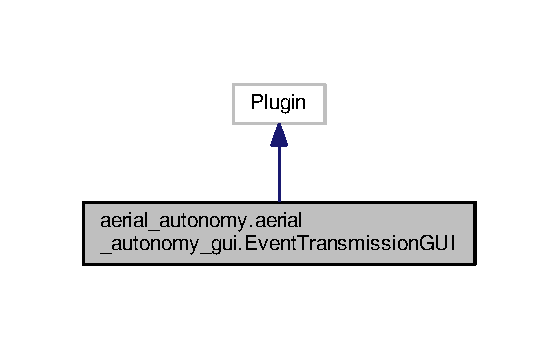
\includegraphics[width=268pt]{classaerial__autonomy_1_1aerial__autonomy__gui_1_1EventTransmissionGUI__inherit__graph}
\end{center}
\end{figure}


Collaboration diagram for aerial\-\_\-autonomy.\-aerial\-\_\-autonomy\-\_\-gui.\-Event\-Transmission\-G\-U\-I\-:\nopagebreak
\begin{figure}[H]
\begin{center}
\leavevmode
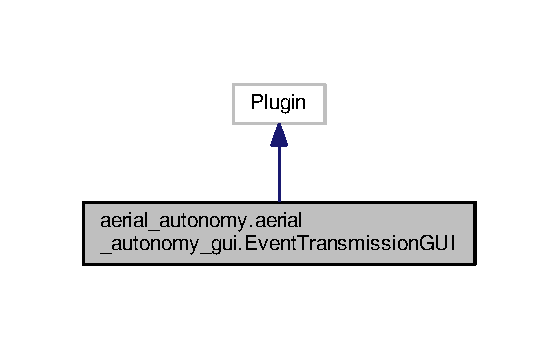
\includegraphics[width=268pt]{classaerial__autonomy_1_1aerial__autonomy__gui_1_1EventTransmissionGUI__coll__graph}
\end{center}
\end{figure}
\subsection*{Public Member Functions}
\begin{DoxyCompactItemize}
\item 
def \hyperlink{classaerial__autonomy_1_1aerial__autonomy__gui_1_1EventTransmissionGUI_a6b65594c62caf4c8cedfbd9f12168dfb}{\-\_\-\-\_\-init\-\_\-\-\_\-}
\begin{DoxyCompactList}\small\item\em Create Qt G\-U\-I using the event file. \end{DoxyCompactList}\item 
def \hyperlink{classaerial__autonomy_1_1aerial__autonomy__gui_1_1EventTransmissionGUI_a10f2fd3747b7f899efde6ff0c67d95b6}{get\-\_\-row\-\_\-col}
\begin{DoxyCompactList}\small\item\em Automatically find the row and col to add the button to in a grid based on index of the button. \end{DoxyCompactList}\item 
def \hyperlink{classaerial__autonomy_1_1aerial__autonomy__gui_1_1EventTransmissionGUI_a9b9a66142bcd76a1be23682c7fdd424a}{pose\-Command\-Callback}
\begin{DoxyCompactList}\small\item\em Saves pose command and updates command display. \end{DoxyCompactList}\item 
def \hyperlink{classaerial__autonomy_1_1aerial__autonomy__gui_1_1EventTransmissionGUI_ae276f79545a8707c09bf07cf51132ef7}{pose\-Command\-Button\-Callback}
\begin{DoxyCompactList}\small\item\em Publishes stored pose command after setting height from slider. \end{DoxyCompactList}\item 
def \hyperlink{classaerial__autonomy_1_1aerial__autonomy__gui_1_1EventTransmissionGUI_aaa8ae13ff7e5ad9128ae565cecd49427}{update\-Height}
\begin{DoxyCompactList}\small\item\em Updates height label based on slider value. \end{DoxyCompactList}\item 
def \hyperlink{classaerial__autonomy_1_1aerial__autonomy__gui_1_1EventTransmissionGUI_a21d7d7031e8de77b2e31e7edb5936a34}{update\-Status}
\begin{DoxyCompactList}\small\item\em Generic placeholder function to update text box. \end{DoxyCompactList}\end{DoxyCompactItemize}
\subsection*{Static Public Member Functions}
\begin{DoxyCompactItemize}
\item 
def \hyperlink{classaerial__autonomy_1_1aerial__autonomy__gui_1_1EventTransmissionGUI_adffec416c73f6f719e9592d0e2286c8f}{add\-\_\-arguments}
\begin{DoxyCompactList}\small\item\em Notify rqt\-\_\-gui that this plugin can parse these extra arguments. \end{DoxyCompactList}\end{DoxyCompactItemize}
\subsection*{Public Attributes}
\begin{DoxyCompactItemize}
\item 
\hyperlink{classaerial__autonomy_1_1aerial__autonomy__gui_1_1EventTransmissionGUI_a28f1de5a0d232285414764f25e43a7eb}{event\-\_\-trigger}
\begin{DoxyCompactList}\small\item\em Create Event trigger. \end{DoxyCompactList}\item 
\hyperlink{classaerial__autonomy_1_1aerial__autonomy__gui_1_1EventTransmissionGUI_a2e96f52dc90edde242b5387214a82858}{system\-\_\-status\-\_\-textbox}
\begin{DoxyCompactList}\small\item\em Textbox to show sytem status. \end{DoxyCompactList}\item 
\hyperlink{classaerial__autonomy_1_1aerial__autonomy__gui_1_1EventTransmissionGUI_a6118098a267761831ef8d83cbf2a78bd}{height\-\_\-slider}
\begin{DoxyCompactList}\small\item\em Height slider to adjust z coordinate for pose command. \end{DoxyCompactList}\item 
\hyperlink{classaerial__autonomy_1_1aerial__autonomy__gui_1_1EventTransmissionGUI_af611df98da28aba90ce5fcbea285603a}{pose\-\_\-command\-\_\-container}
\begin{DoxyCompactList}\small\item\em Container for pose event related objects\-: slide etc. \end{DoxyCompactList}\item 
\hyperlink{classaerial__autonomy_1_1aerial__autonomy__gui_1_1EventTransmissionGUI_a966d066bb1db4ea2517dc68335b3df98}{pose\-\_\-command\-\_\-layout}
\begin{DoxyCompactList}\small\item\em Pose command layout. \end{DoxyCompactList}\item 
\hyperlink{classaerial__autonomy_1_1aerial__autonomy__gui_1_1EventTransmissionGUI_a750b19ad6b27411d6ff502aa4ba43ed8}{pose\-\_\-x}
\begin{DoxyCompactList}\small\item\em x pose label to display position command from rviz to user \end{DoxyCompactList}\item 
\hyperlink{classaerial__autonomy_1_1aerial__autonomy__gui_1_1EventTransmissionGUI_a279bc7aaaf956e4fc14ad3e62bf7b4d2}{pose\-\_\-y}
\begin{DoxyCompactList}\small\item\em y pose label to display position command from rviz to user \end{DoxyCompactList}\item 
\hyperlink{classaerial__autonomy_1_1aerial__autonomy__gui_1_1EventTransmissionGUI_aead4d11a8fe43596a7077554542af0d2}{pose\-\_\-z}
\begin{DoxyCompactList}\small\item\em z pose label to display position command from rviz to user \end{DoxyCompactList}\item 
\hyperlink{classaerial__autonomy_1_1aerial__autonomy__gui_1_1EventTransmissionGUI_aa82ebdb0e64df86776b6cd9aacecb350}{send\-\_\-pose\-\_\-command\-\_\-button}
\begin{DoxyCompactList}\small\item\em Button to send the pose command to state machine as poseyaw event. \end{DoxyCompactList}\item 
\hyperlink{classaerial__autonomy_1_1aerial__autonomy__gui_1_1EventTransmissionGUI_acedbac17d93e4e743b8bef847720659f}{pose\-\_\-command}
\begin{DoxyCompactList}\small\item\em Pose command container to store pose from Rviz and send to state machine. \end{DoxyCompactList}\item 
\hyperlink{classaerial__autonomy_1_1aerial__autonomy__gui_1_1EventTransmissionGUI_a21ccb12c6c1d93f2d70ccca1c741ec73}{button\-\_\-container}
\begin{DoxyCompactList}\small\item\em Continer to store event triggering buttons. \end{DoxyCompactList}\item 
\hyperlink{classaerial__autonomy_1_1aerial__autonomy__gui_1_1EventTransmissionGUI_a9b589c667ce4f5719c5bb0ddbdb0fd42}{push\-\_\-buttons}
\begin{DoxyCompactList}\small\item\em List of push buttons to trigger events. \end{DoxyCompactList}\item 
\hyperlink{classaerial__autonomy_1_1aerial__autonomy__gui_1_1EventTransmissionGUI_a1a4f6c154f52187c5b6206cb327b1ebc}{button\-\_\-layout}
\begin{DoxyCompactList}\small\item\em Layout for the push buttons. \end{DoxyCompactList}\end{DoxyCompactItemize}


\subsection{Detailed Description}
G\-U\-I to send events from User to logic state machine. 

\subsection{Constructor \& Destructor Documentation}
\hypertarget{classaerial__autonomy_1_1aerial__autonomy__gui_1_1EventTransmissionGUI_a6b65594c62caf4c8cedfbd9f12168dfb}{\index{aerial\-\_\-autonomy\-::aerial\-\_\-autonomy\-\_\-gui\-::\-Event\-Transmission\-G\-U\-I@{aerial\-\_\-autonomy\-::aerial\-\_\-autonomy\-\_\-gui\-::\-Event\-Transmission\-G\-U\-I}!\-\_\-\-\_\-init\-\_\-\-\_\-@{\-\_\-\-\_\-init\-\_\-\-\_\-}}
\index{\-\_\-\-\_\-init\-\_\-\-\_\-@{\-\_\-\-\_\-init\-\_\-\-\_\-}!aerial_autonomy::aerial_autonomy_gui::EventTransmissionGUI@{aerial\-\_\-autonomy\-::aerial\-\_\-autonomy\-\_\-gui\-::\-Event\-Transmission\-G\-U\-I}}
\subsubsection[{\-\_\-\-\_\-init\-\_\-\-\_\-}]{\setlength{\rightskip}{0pt plus 5cm}def aerial\-\_\-autonomy.\-aerial\-\_\-autonomy\-\_\-gui.\-Event\-Transmission\-G\-U\-I.\-\_\-\-\_\-init\-\_\-\-\_\- (
\begin{DoxyParamCaption}
\item[{}]{self, }
\item[{}]{context}
\end{DoxyParamCaption}
)}}\label{classaerial__autonomy_1_1aerial__autonomy__gui_1_1EventTransmissionGUI_a6b65594c62caf4c8cedfbd9f12168dfb}


Create Qt G\-U\-I using the event file. 



\subsection{Member Function Documentation}
\hypertarget{classaerial__autonomy_1_1aerial__autonomy__gui_1_1EventTransmissionGUI_adffec416c73f6f719e9592d0e2286c8f}{\index{aerial\-\_\-autonomy\-::aerial\-\_\-autonomy\-\_\-gui\-::\-Event\-Transmission\-G\-U\-I@{aerial\-\_\-autonomy\-::aerial\-\_\-autonomy\-\_\-gui\-::\-Event\-Transmission\-G\-U\-I}!add\-\_\-arguments@{add\-\_\-arguments}}
\index{add\-\_\-arguments@{add\-\_\-arguments}!aerial_autonomy::aerial_autonomy_gui::EventTransmissionGUI@{aerial\-\_\-autonomy\-::aerial\-\_\-autonomy\-\_\-gui\-::\-Event\-Transmission\-G\-U\-I}}
\subsubsection[{add\-\_\-arguments}]{\setlength{\rightskip}{0pt plus 5cm}def aerial\-\_\-autonomy.\-aerial\-\_\-autonomy\-\_\-gui.\-Event\-Transmission\-G\-U\-I.\-add\-\_\-arguments (
\begin{DoxyParamCaption}
\item[{}]{parser}
\end{DoxyParamCaption}
)\hspace{0.3cm}{\ttfamily [static]}}}\label{classaerial__autonomy_1_1aerial__autonomy__gui_1_1EventTransmissionGUI_adffec416c73f6f719e9592d0e2286c8f}


Notify rqt\-\_\-gui that this plugin can parse these extra arguments. 

\hypertarget{classaerial__autonomy_1_1aerial__autonomy__gui_1_1EventTransmissionGUI_a10f2fd3747b7f899efde6ff0c67d95b6}{\index{aerial\-\_\-autonomy\-::aerial\-\_\-autonomy\-\_\-gui\-::\-Event\-Transmission\-G\-U\-I@{aerial\-\_\-autonomy\-::aerial\-\_\-autonomy\-\_\-gui\-::\-Event\-Transmission\-G\-U\-I}!get\-\_\-row\-\_\-col@{get\-\_\-row\-\_\-col}}
\index{get\-\_\-row\-\_\-col@{get\-\_\-row\-\_\-col}!aerial_autonomy::aerial_autonomy_gui::EventTransmissionGUI@{aerial\-\_\-autonomy\-::aerial\-\_\-autonomy\-\_\-gui\-::\-Event\-Transmission\-G\-U\-I}}
\subsubsection[{get\-\_\-row\-\_\-col}]{\setlength{\rightskip}{0pt plus 5cm}def aerial\-\_\-autonomy.\-aerial\-\_\-autonomy\-\_\-gui.\-Event\-Transmission\-G\-U\-I.\-get\-\_\-row\-\_\-col (
\begin{DoxyParamCaption}
\item[{}]{self, }
\item[{}]{button\-\_\-index, }
\item[{}]{ncols}
\end{DoxyParamCaption}
)}}\label{classaerial__autonomy_1_1aerial__autonomy__gui_1_1EventTransmissionGUI_a10f2fd3747b7f899efde6ff0c67d95b6}


Automatically find the row and col to add the button to in a grid based on index of the button. 

\hypertarget{classaerial__autonomy_1_1aerial__autonomy__gui_1_1EventTransmissionGUI_ae276f79545a8707c09bf07cf51132ef7}{\index{aerial\-\_\-autonomy\-::aerial\-\_\-autonomy\-\_\-gui\-::\-Event\-Transmission\-G\-U\-I@{aerial\-\_\-autonomy\-::aerial\-\_\-autonomy\-\_\-gui\-::\-Event\-Transmission\-G\-U\-I}!pose\-Command\-Button\-Callback@{pose\-Command\-Button\-Callback}}
\index{pose\-Command\-Button\-Callback@{pose\-Command\-Button\-Callback}!aerial_autonomy::aerial_autonomy_gui::EventTransmissionGUI@{aerial\-\_\-autonomy\-::aerial\-\_\-autonomy\-\_\-gui\-::\-Event\-Transmission\-G\-U\-I}}
\subsubsection[{pose\-Command\-Button\-Callback}]{\setlength{\rightskip}{0pt plus 5cm}def aerial\-\_\-autonomy.\-aerial\-\_\-autonomy\-\_\-gui.\-Event\-Transmission\-G\-U\-I.\-pose\-Command\-Button\-Callback (
\begin{DoxyParamCaption}
\item[{}]{self}
\end{DoxyParamCaption}
)}}\label{classaerial__autonomy_1_1aerial__autonomy__gui_1_1EventTransmissionGUI_ae276f79545a8707c09bf07cf51132ef7}


Publishes stored pose command after setting height from slider. 

\hypertarget{classaerial__autonomy_1_1aerial__autonomy__gui_1_1EventTransmissionGUI_a9b9a66142bcd76a1be23682c7fdd424a}{\index{aerial\-\_\-autonomy\-::aerial\-\_\-autonomy\-\_\-gui\-::\-Event\-Transmission\-G\-U\-I@{aerial\-\_\-autonomy\-::aerial\-\_\-autonomy\-\_\-gui\-::\-Event\-Transmission\-G\-U\-I}!pose\-Command\-Callback@{pose\-Command\-Callback}}
\index{pose\-Command\-Callback@{pose\-Command\-Callback}!aerial_autonomy::aerial_autonomy_gui::EventTransmissionGUI@{aerial\-\_\-autonomy\-::aerial\-\_\-autonomy\-\_\-gui\-::\-Event\-Transmission\-G\-U\-I}}
\subsubsection[{pose\-Command\-Callback}]{\setlength{\rightskip}{0pt plus 5cm}def aerial\-\_\-autonomy.\-aerial\-\_\-autonomy\-\_\-gui.\-Event\-Transmission\-G\-U\-I.\-pose\-Command\-Callback (
\begin{DoxyParamCaption}
\item[{}]{self, }
\item[{}]{pose}
\end{DoxyParamCaption}
)}}\label{classaerial__autonomy_1_1aerial__autonomy__gui_1_1EventTransmissionGUI_a9b9a66142bcd76a1be23682c7fdd424a}


Saves pose command and updates command display. 

\hypertarget{classaerial__autonomy_1_1aerial__autonomy__gui_1_1EventTransmissionGUI_aaa8ae13ff7e5ad9128ae565cecd49427}{\index{aerial\-\_\-autonomy\-::aerial\-\_\-autonomy\-\_\-gui\-::\-Event\-Transmission\-G\-U\-I@{aerial\-\_\-autonomy\-::aerial\-\_\-autonomy\-\_\-gui\-::\-Event\-Transmission\-G\-U\-I}!update\-Height@{update\-Height}}
\index{update\-Height@{update\-Height}!aerial_autonomy::aerial_autonomy_gui::EventTransmissionGUI@{aerial\-\_\-autonomy\-::aerial\-\_\-autonomy\-\_\-gui\-::\-Event\-Transmission\-G\-U\-I}}
\subsubsection[{update\-Height}]{\setlength{\rightskip}{0pt plus 5cm}def aerial\-\_\-autonomy.\-aerial\-\_\-autonomy\-\_\-gui.\-Event\-Transmission\-G\-U\-I.\-update\-Height (
\begin{DoxyParamCaption}
\item[{}]{self}
\end{DoxyParamCaption}
)}}\label{classaerial__autonomy_1_1aerial__autonomy__gui_1_1EventTransmissionGUI_aaa8ae13ff7e5ad9128ae565cecd49427}


Updates height label based on slider value. 

\hypertarget{classaerial__autonomy_1_1aerial__autonomy__gui_1_1EventTransmissionGUI_a21d7d7031e8de77b2e31e7edb5936a34}{\index{aerial\-\_\-autonomy\-::aerial\-\_\-autonomy\-\_\-gui\-::\-Event\-Transmission\-G\-U\-I@{aerial\-\_\-autonomy\-::aerial\-\_\-autonomy\-\_\-gui\-::\-Event\-Transmission\-G\-U\-I}!update\-Status@{update\-Status}}
\index{update\-Status@{update\-Status}!aerial_autonomy::aerial_autonomy_gui::EventTransmissionGUI@{aerial\-\_\-autonomy\-::aerial\-\_\-autonomy\-\_\-gui\-::\-Event\-Transmission\-G\-U\-I}}
\subsubsection[{update\-Status}]{\setlength{\rightskip}{0pt plus 5cm}def aerial\-\_\-autonomy.\-aerial\-\_\-autonomy\-\_\-gui.\-Event\-Transmission\-G\-U\-I.\-update\-Status (
\begin{DoxyParamCaption}
\item[{}]{self, }
\item[{}]{status, }
\item[{}]{text\-\_\-box}
\end{DoxyParamCaption}
)}}\label{classaerial__autonomy_1_1aerial__autonomy__gui_1_1EventTransmissionGUI_a21d7d7031e8de77b2e31e7edb5936a34}


Generic placeholder function to update text box. 



\subsection{Member Data Documentation}
\hypertarget{classaerial__autonomy_1_1aerial__autonomy__gui_1_1EventTransmissionGUI_a21ccb12c6c1d93f2d70ccca1c741ec73}{\index{aerial\-\_\-autonomy\-::aerial\-\_\-autonomy\-\_\-gui\-::\-Event\-Transmission\-G\-U\-I@{aerial\-\_\-autonomy\-::aerial\-\_\-autonomy\-\_\-gui\-::\-Event\-Transmission\-G\-U\-I}!button\-\_\-container@{button\-\_\-container}}
\index{button\-\_\-container@{button\-\_\-container}!aerial_autonomy::aerial_autonomy_gui::EventTransmissionGUI@{aerial\-\_\-autonomy\-::aerial\-\_\-autonomy\-\_\-gui\-::\-Event\-Transmission\-G\-U\-I}}
\subsubsection[{button\-\_\-container}]{\setlength{\rightskip}{0pt plus 5cm}aerial\-\_\-autonomy.\-aerial\-\_\-autonomy\-\_\-gui.\-Event\-Transmission\-G\-U\-I.\-button\-\_\-container}}\label{classaerial__autonomy_1_1aerial__autonomy__gui_1_1EventTransmissionGUI_a21ccb12c6c1d93f2d70ccca1c741ec73}


Continer to store event triggering buttons. 

\hypertarget{classaerial__autonomy_1_1aerial__autonomy__gui_1_1EventTransmissionGUI_a1a4f6c154f52187c5b6206cb327b1ebc}{\index{aerial\-\_\-autonomy\-::aerial\-\_\-autonomy\-\_\-gui\-::\-Event\-Transmission\-G\-U\-I@{aerial\-\_\-autonomy\-::aerial\-\_\-autonomy\-\_\-gui\-::\-Event\-Transmission\-G\-U\-I}!button\-\_\-layout@{button\-\_\-layout}}
\index{button\-\_\-layout@{button\-\_\-layout}!aerial_autonomy::aerial_autonomy_gui::EventTransmissionGUI@{aerial\-\_\-autonomy\-::aerial\-\_\-autonomy\-\_\-gui\-::\-Event\-Transmission\-G\-U\-I}}
\subsubsection[{button\-\_\-layout}]{\setlength{\rightskip}{0pt plus 5cm}aerial\-\_\-autonomy.\-aerial\-\_\-autonomy\-\_\-gui.\-Event\-Transmission\-G\-U\-I.\-button\-\_\-layout}}\label{classaerial__autonomy_1_1aerial__autonomy__gui_1_1EventTransmissionGUI_a1a4f6c154f52187c5b6206cb327b1ebc}


Layout for the push buttons. 

\hypertarget{classaerial__autonomy_1_1aerial__autonomy__gui_1_1EventTransmissionGUI_a28f1de5a0d232285414764f25e43a7eb}{\index{aerial\-\_\-autonomy\-::aerial\-\_\-autonomy\-\_\-gui\-::\-Event\-Transmission\-G\-U\-I@{aerial\-\_\-autonomy\-::aerial\-\_\-autonomy\-\_\-gui\-::\-Event\-Transmission\-G\-U\-I}!event\-\_\-trigger@{event\-\_\-trigger}}
\index{event\-\_\-trigger@{event\-\_\-trigger}!aerial_autonomy::aerial_autonomy_gui::EventTransmissionGUI@{aerial\-\_\-autonomy\-::aerial\-\_\-autonomy\-\_\-gui\-::\-Event\-Transmission\-G\-U\-I}}
\subsubsection[{event\-\_\-trigger}]{\setlength{\rightskip}{0pt plus 5cm}aerial\-\_\-autonomy.\-aerial\-\_\-autonomy\-\_\-gui.\-Event\-Transmission\-G\-U\-I.\-event\-\_\-trigger}}\label{classaerial__autonomy_1_1aerial__autonomy__gui_1_1EventTransmissionGUI_a28f1de5a0d232285414764f25e43a7eb}


Create Event trigger. 

\hypertarget{classaerial__autonomy_1_1aerial__autonomy__gui_1_1EventTransmissionGUI_a6118098a267761831ef8d83cbf2a78bd}{\index{aerial\-\_\-autonomy\-::aerial\-\_\-autonomy\-\_\-gui\-::\-Event\-Transmission\-G\-U\-I@{aerial\-\_\-autonomy\-::aerial\-\_\-autonomy\-\_\-gui\-::\-Event\-Transmission\-G\-U\-I}!height\-\_\-slider@{height\-\_\-slider}}
\index{height\-\_\-slider@{height\-\_\-slider}!aerial_autonomy::aerial_autonomy_gui::EventTransmissionGUI@{aerial\-\_\-autonomy\-::aerial\-\_\-autonomy\-\_\-gui\-::\-Event\-Transmission\-G\-U\-I}}
\subsubsection[{height\-\_\-slider}]{\setlength{\rightskip}{0pt plus 5cm}aerial\-\_\-autonomy.\-aerial\-\_\-autonomy\-\_\-gui.\-Event\-Transmission\-G\-U\-I.\-height\-\_\-slider}}\label{classaerial__autonomy_1_1aerial__autonomy__gui_1_1EventTransmissionGUI_a6118098a267761831ef8d83cbf2a78bd}


Height slider to adjust z coordinate for pose command. 

\begin{DoxyRefDesc}{Todo}
\item[\hyperlink{todo__todo000001}{Todo}]Matt\-: Load slider settings from param file \end{DoxyRefDesc}
\hypertarget{classaerial__autonomy_1_1aerial__autonomy__gui_1_1EventTransmissionGUI_acedbac17d93e4e743b8bef847720659f}{\index{aerial\-\_\-autonomy\-::aerial\-\_\-autonomy\-\_\-gui\-::\-Event\-Transmission\-G\-U\-I@{aerial\-\_\-autonomy\-::aerial\-\_\-autonomy\-\_\-gui\-::\-Event\-Transmission\-G\-U\-I}!pose\-\_\-command@{pose\-\_\-command}}
\index{pose\-\_\-command@{pose\-\_\-command}!aerial_autonomy::aerial_autonomy_gui::EventTransmissionGUI@{aerial\-\_\-autonomy\-::aerial\-\_\-autonomy\-\_\-gui\-::\-Event\-Transmission\-G\-U\-I}}
\subsubsection[{pose\-\_\-command}]{\setlength{\rightskip}{0pt plus 5cm}aerial\-\_\-autonomy.\-aerial\-\_\-autonomy\-\_\-gui.\-Event\-Transmission\-G\-U\-I.\-pose\-\_\-command}}\label{classaerial__autonomy_1_1aerial__autonomy__gui_1_1EventTransmissionGUI_acedbac17d93e4e743b8bef847720659f}


Pose command container to store pose from Rviz and send to state machine. 

\hypertarget{classaerial__autonomy_1_1aerial__autonomy__gui_1_1EventTransmissionGUI_af611df98da28aba90ce5fcbea285603a}{\index{aerial\-\_\-autonomy\-::aerial\-\_\-autonomy\-\_\-gui\-::\-Event\-Transmission\-G\-U\-I@{aerial\-\_\-autonomy\-::aerial\-\_\-autonomy\-\_\-gui\-::\-Event\-Transmission\-G\-U\-I}!pose\-\_\-command\-\_\-container@{pose\-\_\-command\-\_\-container}}
\index{pose\-\_\-command\-\_\-container@{pose\-\_\-command\-\_\-container}!aerial_autonomy::aerial_autonomy_gui::EventTransmissionGUI@{aerial\-\_\-autonomy\-::aerial\-\_\-autonomy\-\_\-gui\-::\-Event\-Transmission\-G\-U\-I}}
\subsubsection[{pose\-\_\-command\-\_\-container}]{\setlength{\rightskip}{0pt plus 5cm}aerial\-\_\-autonomy.\-aerial\-\_\-autonomy\-\_\-gui.\-Event\-Transmission\-G\-U\-I.\-pose\-\_\-command\-\_\-container}}\label{classaerial__autonomy_1_1aerial__autonomy__gui_1_1EventTransmissionGUI_af611df98da28aba90ce5fcbea285603a}


Container for pose event related objects\-: slide etc. 

\begin{DoxyRefDesc}{Todo}
\item[\hyperlink{todo__todo000002}{Todo}]Matt\-: Reset slider value based on current quad height \end{DoxyRefDesc}
\hypertarget{classaerial__autonomy_1_1aerial__autonomy__gui_1_1EventTransmissionGUI_a966d066bb1db4ea2517dc68335b3df98}{\index{aerial\-\_\-autonomy\-::aerial\-\_\-autonomy\-\_\-gui\-::\-Event\-Transmission\-G\-U\-I@{aerial\-\_\-autonomy\-::aerial\-\_\-autonomy\-\_\-gui\-::\-Event\-Transmission\-G\-U\-I}!pose\-\_\-command\-\_\-layout@{pose\-\_\-command\-\_\-layout}}
\index{pose\-\_\-command\-\_\-layout@{pose\-\_\-command\-\_\-layout}!aerial_autonomy::aerial_autonomy_gui::EventTransmissionGUI@{aerial\-\_\-autonomy\-::aerial\-\_\-autonomy\-\_\-gui\-::\-Event\-Transmission\-G\-U\-I}}
\subsubsection[{pose\-\_\-command\-\_\-layout}]{\setlength{\rightskip}{0pt plus 5cm}aerial\-\_\-autonomy.\-aerial\-\_\-autonomy\-\_\-gui.\-Event\-Transmission\-G\-U\-I.\-pose\-\_\-command\-\_\-layout}}\label{classaerial__autonomy_1_1aerial__autonomy__gui_1_1EventTransmissionGUI_a966d066bb1db4ea2517dc68335b3df98}


Pose command layout. 

\hypertarget{classaerial__autonomy_1_1aerial__autonomy__gui_1_1EventTransmissionGUI_a750b19ad6b27411d6ff502aa4ba43ed8}{\index{aerial\-\_\-autonomy\-::aerial\-\_\-autonomy\-\_\-gui\-::\-Event\-Transmission\-G\-U\-I@{aerial\-\_\-autonomy\-::aerial\-\_\-autonomy\-\_\-gui\-::\-Event\-Transmission\-G\-U\-I}!pose\-\_\-x@{pose\-\_\-x}}
\index{pose\-\_\-x@{pose\-\_\-x}!aerial_autonomy::aerial_autonomy_gui::EventTransmissionGUI@{aerial\-\_\-autonomy\-::aerial\-\_\-autonomy\-\_\-gui\-::\-Event\-Transmission\-G\-U\-I}}
\subsubsection[{pose\-\_\-x}]{\setlength{\rightskip}{0pt plus 5cm}aerial\-\_\-autonomy.\-aerial\-\_\-autonomy\-\_\-gui.\-Event\-Transmission\-G\-U\-I.\-pose\-\_\-x}}\label{classaerial__autonomy_1_1aerial__autonomy__gui_1_1EventTransmissionGUI_a750b19ad6b27411d6ff502aa4ba43ed8}


x pose label to display position command from rviz to user 

\hypertarget{classaerial__autonomy_1_1aerial__autonomy__gui_1_1EventTransmissionGUI_a279bc7aaaf956e4fc14ad3e62bf7b4d2}{\index{aerial\-\_\-autonomy\-::aerial\-\_\-autonomy\-\_\-gui\-::\-Event\-Transmission\-G\-U\-I@{aerial\-\_\-autonomy\-::aerial\-\_\-autonomy\-\_\-gui\-::\-Event\-Transmission\-G\-U\-I}!pose\-\_\-y@{pose\-\_\-y}}
\index{pose\-\_\-y@{pose\-\_\-y}!aerial_autonomy::aerial_autonomy_gui::EventTransmissionGUI@{aerial\-\_\-autonomy\-::aerial\-\_\-autonomy\-\_\-gui\-::\-Event\-Transmission\-G\-U\-I}}
\subsubsection[{pose\-\_\-y}]{\setlength{\rightskip}{0pt plus 5cm}aerial\-\_\-autonomy.\-aerial\-\_\-autonomy\-\_\-gui.\-Event\-Transmission\-G\-U\-I.\-pose\-\_\-y}}\label{classaerial__autonomy_1_1aerial__autonomy__gui_1_1EventTransmissionGUI_a279bc7aaaf956e4fc14ad3e62bf7b4d2}


y pose label to display position command from rviz to user 

\hypertarget{classaerial__autonomy_1_1aerial__autonomy__gui_1_1EventTransmissionGUI_aead4d11a8fe43596a7077554542af0d2}{\index{aerial\-\_\-autonomy\-::aerial\-\_\-autonomy\-\_\-gui\-::\-Event\-Transmission\-G\-U\-I@{aerial\-\_\-autonomy\-::aerial\-\_\-autonomy\-\_\-gui\-::\-Event\-Transmission\-G\-U\-I}!pose\-\_\-z@{pose\-\_\-z}}
\index{pose\-\_\-z@{pose\-\_\-z}!aerial_autonomy::aerial_autonomy_gui::EventTransmissionGUI@{aerial\-\_\-autonomy\-::aerial\-\_\-autonomy\-\_\-gui\-::\-Event\-Transmission\-G\-U\-I}}
\subsubsection[{pose\-\_\-z}]{\setlength{\rightskip}{0pt plus 5cm}aerial\-\_\-autonomy.\-aerial\-\_\-autonomy\-\_\-gui.\-Event\-Transmission\-G\-U\-I.\-pose\-\_\-z}}\label{classaerial__autonomy_1_1aerial__autonomy__gui_1_1EventTransmissionGUI_aead4d11a8fe43596a7077554542af0d2}


z pose label to display position command from rviz to user 

\hypertarget{classaerial__autonomy_1_1aerial__autonomy__gui_1_1EventTransmissionGUI_a9b589c667ce4f5719c5bb0ddbdb0fd42}{\index{aerial\-\_\-autonomy\-::aerial\-\_\-autonomy\-\_\-gui\-::\-Event\-Transmission\-G\-U\-I@{aerial\-\_\-autonomy\-::aerial\-\_\-autonomy\-\_\-gui\-::\-Event\-Transmission\-G\-U\-I}!push\-\_\-buttons@{push\-\_\-buttons}}
\index{push\-\_\-buttons@{push\-\_\-buttons}!aerial_autonomy::aerial_autonomy_gui::EventTransmissionGUI@{aerial\-\_\-autonomy\-::aerial\-\_\-autonomy\-\_\-gui\-::\-Event\-Transmission\-G\-U\-I}}
\subsubsection[{push\-\_\-buttons}]{\setlength{\rightskip}{0pt plus 5cm}aerial\-\_\-autonomy.\-aerial\-\_\-autonomy\-\_\-gui.\-Event\-Transmission\-G\-U\-I.\-push\-\_\-buttons}}\label{classaerial__autonomy_1_1aerial__autonomy__gui_1_1EventTransmissionGUI_a9b589c667ce4f5719c5bb0ddbdb0fd42}


List of push buttons to trigger events. 

\hypertarget{classaerial__autonomy_1_1aerial__autonomy__gui_1_1EventTransmissionGUI_aa82ebdb0e64df86776b6cd9aacecb350}{\index{aerial\-\_\-autonomy\-::aerial\-\_\-autonomy\-\_\-gui\-::\-Event\-Transmission\-G\-U\-I@{aerial\-\_\-autonomy\-::aerial\-\_\-autonomy\-\_\-gui\-::\-Event\-Transmission\-G\-U\-I}!send\-\_\-pose\-\_\-command\-\_\-button@{send\-\_\-pose\-\_\-command\-\_\-button}}
\index{send\-\_\-pose\-\_\-command\-\_\-button@{send\-\_\-pose\-\_\-command\-\_\-button}!aerial_autonomy::aerial_autonomy_gui::EventTransmissionGUI@{aerial\-\_\-autonomy\-::aerial\-\_\-autonomy\-\_\-gui\-::\-Event\-Transmission\-G\-U\-I}}
\subsubsection[{send\-\_\-pose\-\_\-command\-\_\-button}]{\setlength{\rightskip}{0pt plus 5cm}aerial\-\_\-autonomy.\-aerial\-\_\-autonomy\-\_\-gui.\-Event\-Transmission\-G\-U\-I.\-send\-\_\-pose\-\_\-command\-\_\-button}}\label{classaerial__autonomy_1_1aerial__autonomy__gui_1_1EventTransmissionGUI_aa82ebdb0e64df86776b6cd9aacecb350}


Button to send the pose command to state machine as poseyaw event. 

\hypertarget{classaerial__autonomy_1_1aerial__autonomy__gui_1_1EventTransmissionGUI_a2e96f52dc90edde242b5387214a82858}{\index{aerial\-\_\-autonomy\-::aerial\-\_\-autonomy\-\_\-gui\-::\-Event\-Transmission\-G\-U\-I@{aerial\-\_\-autonomy\-::aerial\-\_\-autonomy\-\_\-gui\-::\-Event\-Transmission\-G\-U\-I}!system\-\_\-status\-\_\-textbox@{system\-\_\-status\-\_\-textbox}}
\index{system\-\_\-status\-\_\-textbox@{system\-\_\-status\-\_\-textbox}!aerial_autonomy::aerial_autonomy_gui::EventTransmissionGUI@{aerial\-\_\-autonomy\-::aerial\-\_\-autonomy\-\_\-gui\-::\-Event\-Transmission\-G\-U\-I}}
\subsubsection[{system\-\_\-status\-\_\-textbox}]{\setlength{\rightskip}{0pt plus 5cm}aerial\-\_\-autonomy.\-aerial\-\_\-autonomy\-\_\-gui.\-Event\-Transmission\-G\-U\-I.\-system\-\_\-status\-\_\-textbox}}\label{classaerial__autonomy_1_1aerial__autonomy__gui_1_1EventTransmissionGUI_a2e96f52dc90edde242b5387214a82858}


Textbox to show sytem status. 



The documentation for this class was generated from the following file\-:\begin{DoxyCompactItemize}
\item 
src/aerial\-\_\-autonomy/\hyperlink{aerial__autonomy__gui_8py}{aerial\-\_\-autonomy\-\_\-gui.\-py}\end{DoxyCompactItemize}

\hypertarget{structGuardFunctor}{\section{Guard\-Functor$<$ Event\-T, Robot\-System\-T, Logic\-State\-Machine\-T $>$ Struct Template Reference}
\label{structGuardFunctor}\index{Guard\-Functor$<$ Event\-T, Robot\-System\-T, Logic\-State\-Machine\-T $>$@{Guard\-Functor$<$ Event\-T, Robot\-System\-T, Logic\-State\-Machine\-T $>$}}
}


Action Functor for a given event, robot system, state machine.  




{\ttfamily \#include $<$base\-\_\-functors.\-h$>$}

\subsection*{Public Member Functions}
\begin{DoxyCompactItemize}
\item 
virtual bool \hyperlink{structGuardFunctor_a9f023aa88503d6127cc8280d7dc733b8}{guard} (Event\-T const \&event, Robot\-System\-T \&robot\-\_\-system, Logic\-State\-Machine\-T \&logic\-\_\-state\-\_\-machine)=0
\begin{DoxyCompactList}\small\item\em Override this guard function for different sub classes. This function decides whether to call the run function for each state. \end{DoxyCompactList}\item 
{\footnotesize template$<$class F\-S\-M , class Source\-State , class Target\-State $>$ }\\bool \hyperlink{structGuardFunctor_a42b30d1737ceca71bfe47a9bb525ceda}{operator()} (Event\-T const \&event, F\-S\-M \&logic\-\_\-state\-\_\-machine, Source\-State \&, Target\-State \&)
\begin{DoxyCompactList}\small\item\em operator () Internally calls guard function \end{DoxyCompactList}\item 
virtual \hyperlink{structGuardFunctor_a3876b6e5028dcdc35ac786322e8afca3}{$\sim$\-Guard\-Functor} ()
\begin{DoxyCompactList}\small\item\em Destructor. \end{DoxyCompactList}\end{DoxyCompactItemize}


\subsection{Detailed Description}
\subsubsection*{template$<$class Event\-T, class Robot\-System\-T, class Logic\-State\-Machine\-T$>$struct Guard\-Functor$<$ Event\-T, Robot\-System\-T, Logic\-State\-Machine\-T $>$}

Action Functor for a given event, robot system, state machine. 

This class provides guard function for state transitions Derived states have to implement the specific guard function behavior using this base class.


\begin{DoxyTemplParams}{Template Parameters}
{\em Event\-T} & Event triggering this action \\
\hline
{\em Robot\-System\-T} & The robot system used in the guard check \\
\hline
{\em Logic\-State\-Machine\-T} & The logic state machine used to retrieve robot system \\
\hline
\end{DoxyTemplParams}


\subsection{Constructor \& Destructor Documentation}
\hypertarget{structGuardFunctor_a3876b6e5028dcdc35ac786322e8afca3}{\index{Guard\-Functor@{Guard\-Functor}!$\sim$\-Guard\-Functor@{$\sim$\-Guard\-Functor}}
\index{$\sim$\-Guard\-Functor@{$\sim$\-Guard\-Functor}!GuardFunctor@{Guard\-Functor}}
\subsubsection[{$\sim$\-Guard\-Functor}]{\setlength{\rightskip}{0pt plus 5cm}template$<$class Event\-T, class Robot\-System\-T, class Logic\-State\-Machine\-T$>$ virtual {\bf Guard\-Functor}$<$ Event\-T, Robot\-System\-T, Logic\-State\-Machine\-T $>$\-::$\sim${\bf Guard\-Functor} (
\begin{DoxyParamCaption}
{}
\end{DoxyParamCaption}
)\hspace{0.3cm}{\ttfamily [inline]}, {\ttfamily [virtual]}}}\label{structGuardFunctor_a3876b6e5028dcdc35ac786322e8afca3}


Destructor. 



\subsection{Member Function Documentation}
\hypertarget{structGuardFunctor_a9f023aa88503d6127cc8280d7dc733b8}{\index{Guard\-Functor@{Guard\-Functor}!guard@{guard}}
\index{guard@{guard}!GuardFunctor@{Guard\-Functor}}
\subsubsection[{guard}]{\setlength{\rightskip}{0pt plus 5cm}template$<$class Event\-T, class Robot\-System\-T, class Logic\-State\-Machine\-T$>$ virtual bool {\bf Guard\-Functor}$<$ Event\-T, Robot\-System\-T, Logic\-State\-Machine\-T $>$\-::guard (
\begin{DoxyParamCaption}
\item[{Event\-T const \&}]{event, }
\item[{Robot\-System\-T \&}]{robot\-\_\-system, }
\item[{Logic\-State\-Machine\-T \&}]{logic\-\_\-state\-\_\-machine}
\end{DoxyParamCaption}
)\hspace{0.3cm}{\ttfamily [pure virtual]}}}\label{structGuardFunctor_a9f023aa88503d6127cc8280d7dc733b8}


Override this guard function for different sub classes. This function decides whether to call the run function for each state. 


\begin{DoxyParams}{Parameters}
{\em robot\-\_\-system} & Provides sensor data and allows for controlling hardware \\
\hline
{\em logic\-\_\-state\-\_\-machine} & Backend of logic State Machine. can send events using this. \\
\hline
{\em event} & Event triggering the action \\
\hline
\end{DoxyParams}


Implemented in \hyperlink{structPositionControlTransitionGuardFunctor___ad0334337a349f9964d0ba781e995dad6}{Position\-Control\-Transition\-Guard\-Functor\-\_\-$<$ Logic\-State\-Machine\-T $>$}.

\hypertarget{structGuardFunctor_a42b30d1737ceca71bfe47a9bb525ceda}{\index{Guard\-Functor@{Guard\-Functor}!operator()@{operator()}}
\index{operator()@{operator()}!GuardFunctor@{Guard\-Functor}}
\subsubsection[{operator()}]{\setlength{\rightskip}{0pt plus 5cm}template$<$class Event\-T, class Robot\-System\-T, class Logic\-State\-Machine\-T$>$ template$<$class F\-S\-M , class Source\-State , class Target\-State $>$ bool {\bf Guard\-Functor}$<$ Event\-T, Robot\-System\-T, Logic\-State\-Machine\-T $>$\-::operator() (
\begin{DoxyParamCaption}
\item[{Event\-T const \&}]{event, }
\item[{F\-S\-M \&}]{logic\-\_\-state\-\_\-machine, }
\item[{Source\-State \&}]{, }
\item[{Target\-State \&}]{}
\end{DoxyParamCaption}
)\hspace{0.3cm}{\ttfamily [inline]}}}\label{structGuardFunctor_a42b30d1737ceca71bfe47a9bb525ceda}


operator () Internally calls guard function 


\begin{DoxyParams}{Parameters}
{\em logic\-\_\-state\-\_\-machine} & Backend of logic State Machine. can send events using this. \\
\hline
{\em event} & Event triggering the action \\
\hline
\end{DoxyParams}
\begin{DoxyReturn}{Returns}
the result of checking guard for the state 
\end{DoxyReturn}


The documentation for this struct was generated from the following file\-:\begin{DoxyCompactItemize}
\item 
include/aerial\-\_\-autonomy/actions\-\_\-guards/\hyperlink{base__functors_8h}{base\-\_\-functors.\-h}\end{DoxyCompactItemize}

\hypertarget{structHoveringInternalActionFunctor__}{\section{Hovering\-Internal\-Action\-Functor\-\_\-$<$ Logic\-State\-Machine\-T $>$ Struct Template Reference}
\label{structHoveringInternalActionFunctor__}\index{Hovering\-Internal\-Action\-Functor\-\_\-$<$ Logic\-State\-Machine\-T $>$@{Hovering\-Internal\-Action\-Functor\-\_\-$<$ Logic\-State\-Machine\-T $>$}}
}


Internal action when hovering.  




{\ttfamily \#include $<$hovering\-\_\-functors.\-h$>$}



Inheritance diagram for Hovering\-Internal\-Action\-Functor\-\_\-$<$ Logic\-State\-Machine\-T $>$\-:\nopagebreak
\begin{figure}[H]
\begin{center}
\leavevmode
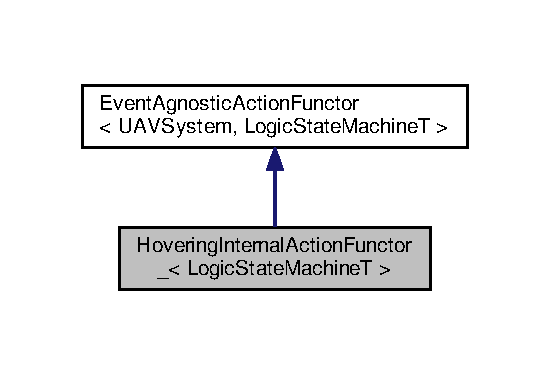
\includegraphics[width=264pt]{structHoveringInternalActionFunctor____inherit__graph}
\end{center}
\end{figure}


Collaboration diagram for Hovering\-Internal\-Action\-Functor\-\_\-$<$ Logic\-State\-Machine\-T $>$\-:\nopagebreak
\begin{figure}[H]
\begin{center}
\leavevmode
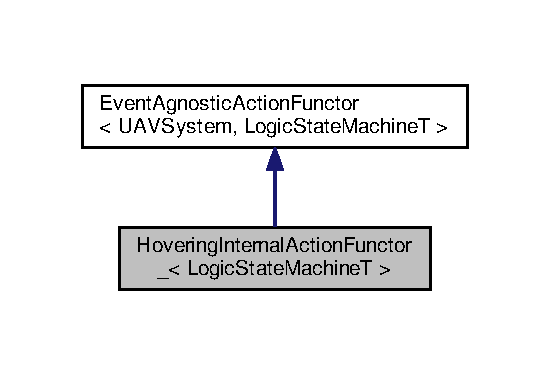
\includegraphics[width=264pt]{structHoveringInternalActionFunctor____coll__graph}
\end{center}
\end{figure}
\subsection*{Public Member Functions}
\begin{DoxyCompactItemize}
\item 
void \hyperlink{structHoveringInternalActionFunctor___a87bb8dd8ed71e54729967b9e258fb66e}{run} (\hyperlink{classUAVSystem}{U\-A\-V\-System} \&robot\-\_\-system, Logic\-State\-Machine\-T \&logic\-\_\-state\-\_\-machine)
\begin{DoxyCompactList}\small\item\em Checks for enough battery voltage and land if battery critical. \end{DoxyCompactList}\end{DoxyCompactItemize}


\subsection{Detailed Description}
\subsubsection*{template$<$class Logic\-State\-Machine\-T$>$struct Hovering\-Internal\-Action\-Functor\-\_\-$<$ Logic\-State\-Machine\-T $>$}

Internal action when hovering. 


\begin{DoxyTemplParams}{Template Parameters}
{\em Logic\-State\-Machine\-T} & Logic state machine used to process events \\
\hline
\end{DoxyTemplParams}


\subsection{Member Function Documentation}
\hypertarget{structHoveringInternalActionFunctor___a87bb8dd8ed71e54729967b9e258fb66e}{\index{Hovering\-Internal\-Action\-Functor\-\_\-@{Hovering\-Internal\-Action\-Functor\-\_\-}!run@{run}}
\index{run@{run}!HoveringInternalActionFunctor_@{Hovering\-Internal\-Action\-Functor\-\_\-}}
\subsubsection[{run}]{\setlength{\rightskip}{0pt plus 5cm}template$<$class Logic\-State\-Machine\-T $>$ void {\bf Hovering\-Internal\-Action\-Functor\-\_\-}$<$ Logic\-State\-Machine\-T $>$\-::run (
\begin{DoxyParamCaption}
\item[{{\bf U\-A\-V\-System} \&}]{robot\-\_\-system, }
\item[{Logic\-State\-Machine\-T \&}]{logic\-\_\-state\-\_\-machine}
\end{DoxyParamCaption}
)\hspace{0.3cm}{\ttfamily [inline]}, {\ttfamily [virtual]}}}\label{structHoveringInternalActionFunctor___a87bb8dd8ed71e54729967b9e258fb66e}


Checks for enough battery voltage and land if battery critical. 


\begin{DoxyParams}{Parameters}
{\em robot\-\_\-system} & robot system to get sensor data \\
\hline
{\em logic\-\_\-state\-\_\-machine} & logic state machine to trigger events \\
\hline
\end{DoxyParams}
\begin{DoxyRefDesc}{Todo}
\item[\hyperlink{todo__todo000005}{Todo}](Gowtham) Can also use uav status here \end{DoxyRefDesc}


Implements \hyperlink{structEventAgnosticActionFunctor_a53a48938d68370ff2ef262222565ffcf}{Event\-Agnostic\-Action\-Functor$<$ U\-A\-V\-System, Logic\-State\-Machine\-T $>$}.



The documentation for this struct was generated from the following file\-:\begin{DoxyCompactItemize}
\item 
include/aerial\-\_\-autonomy/actions\-\_\-guards/\hyperlink{hovering__functors_8h}{hovering\-\_\-functors.\-h}\end{DoxyCompactItemize}

\hypertarget{structBaseState_1_1internal__transition__table}{\section{Base\-State$<$ Robot\-System\-T, Logic\-State\-Machine\-T, Action\-Fctr $>$\-:\-:internal\-\_\-transition\-\_\-table Struct Reference}
\label{structBaseState_1_1internal__transition__table}\index{Base\-State$<$ Robot\-System\-T, Logic\-State\-Machine\-T, Action\-Fctr $>$\-::internal\-\_\-transition\-\_\-table@{Base\-State$<$ Robot\-System\-T, Logic\-State\-Machine\-T, Action\-Fctr $>$\-::internal\-\_\-transition\-\_\-table}}
}


The \hyperlink{structBaseState_1_1internal__transition__table}{internal\-\_\-transition\-\_\-table} to call run function in every state.  




{\ttfamily \#include $<$base\-\_\-state.\-h$>$}



Inheritance diagram for Base\-State$<$ Robot\-System\-T, Logic\-State\-Machine\-T, Action\-Fctr $>$\-:\-:internal\-\_\-transition\-\_\-table\-:\nopagebreak
\begin{figure}[H]
\begin{center}
\leavevmode
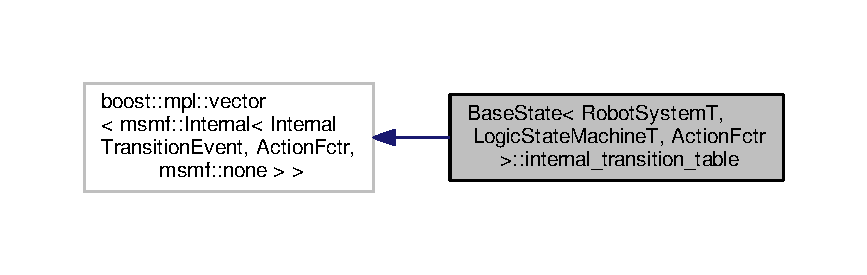
\includegraphics[width=350pt]{structBaseState_1_1internal__transition__table__inherit__graph}
\end{center}
\end{figure}


Collaboration diagram for Base\-State$<$ Robot\-System\-T, Logic\-State\-Machine\-T, Action\-Fctr $>$\-:\-:internal\-\_\-transition\-\_\-table\-:\nopagebreak
\begin{figure}[H]
\begin{center}
\leavevmode
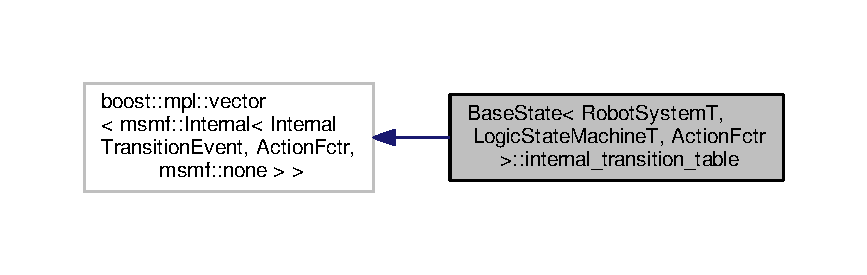
\includegraphics[width=350pt]{structBaseState_1_1internal__transition__table__coll__graph}
\end{center}
\end{figure}


\subsection{Detailed Description}
\subsubsection*{template$<$class Robot\-System\-T, class Logic\-State\-Machine\-T, class Action\-Fctr$>$struct Base\-State$<$ Robot\-System\-T, Logic\-State\-Machine\-T, Action\-Fctr $>$\-::internal\-\_\-transition\-\_\-table}

The \hyperlink{structBaseState_1_1internal__transition__table}{internal\-\_\-transition\-\_\-table} to call run function in every state. 

The documentation for this struct was generated from the following file\-:\begin{DoxyCompactItemize}
\item 
include/aerial\-\_\-autonomy/logic\-\_\-states/\hyperlink{base__state_8h}{base\-\_\-state.\-h}\end{DoxyCompactItemize}

\hypertarget{structLogicStateMachineFrontEnd_1_1Landed_1_1internal__transition__table}{\section{Logic\-State\-Machine\-Front\-End\-:\-:Landed\-:\-:internal\-\_\-transition\-\_\-table Struct Reference}
\label{structLogicStateMachineFrontEnd_1_1Landed_1_1internal__transition__table}\index{Logic\-State\-Machine\-Front\-End\-::\-Landed\-::internal\-\_\-transition\-\_\-table@{Logic\-State\-Machine\-Front\-End\-::\-Landed\-::internal\-\_\-transition\-\_\-table}}
}


Internal event without any action.  




{\ttfamily \#include $<$basic\-\_\-state\-\_\-machine.\-h$>$}



Inheritance diagram for Logic\-State\-Machine\-Front\-End\-:\-:Landed\-:\-:internal\-\_\-transition\-\_\-table\-:\nopagebreak
\begin{figure}[H]
\begin{center}
\leavevmode
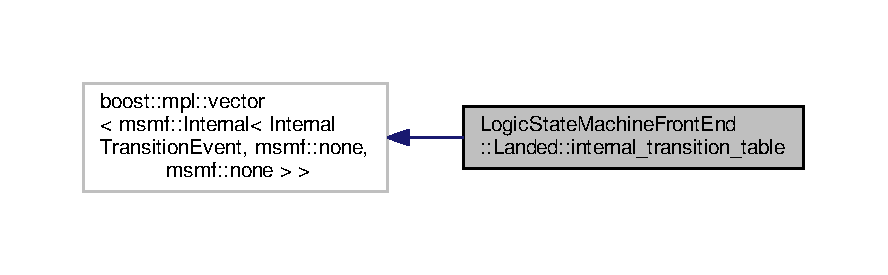
\includegraphics[width=350pt]{structLogicStateMachineFrontEnd_1_1Landed_1_1internal__transition__table__inherit__graph}
\end{center}
\end{figure}


Collaboration diagram for Logic\-State\-Machine\-Front\-End\-:\-:Landed\-:\-:internal\-\_\-transition\-\_\-table\-:\nopagebreak
\begin{figure}[H]
\begin{center}
\leavevmode
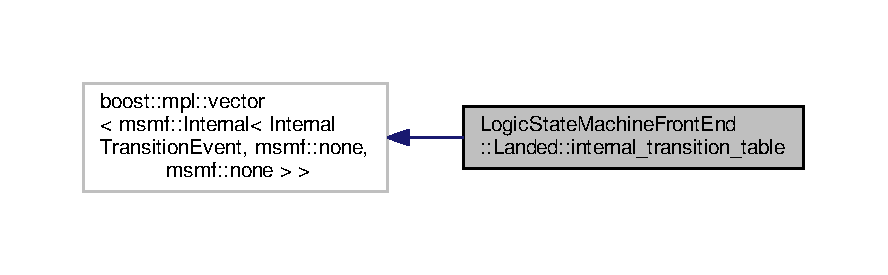
\includegraphics[width=350pt]{structLogicStateMachineFrontEnd_1_1Landed_1_1internal__transition__table__coll__graph}
\end{center}
\end{figure}


\subsection{Detailed Description}
Internal event without any action. 

The documentation for this struct was generated from the following file\-:\begin{DoxyCompactItemize}
\item 
include/aerial\-\_\-autonomy/state\-\_\-machines/\hyperlink{basic__state__machine_8h}{basic\-\_\-state\-\_\-machine.\-h}\end{DoxyCompactItemize}

\hypertarget{structInternalTransitionEvent}{\section{Internal\-Transition\-Event Struct Reference}
\label{structInternalTransitionEvent}\index{Internal\-Transition\-Event@{Internal\-Transition\-Event}}
}


The \hyperlink{structInternalTransitionEvent}{Internal\-Transition\-Event} struct used to trigger action behaviors in states.  




{\ttfamily \#include $<$base\-\_\-functors.\-h$>$}



\subsection{Detailed Description}
The \hyperlink{structInternalTransitionEvent}{Internal\-Transition\-Event} struct used to trigger action behaviors in states. 

The documentation for this struct was generated from the following file\-:\begin{DoxyCompactItemize}
\item 
include/aerial\-\_\-autonomy/actions\-\_\-guards/\hyperlink{base__functors_8h}{base\-\_\-functors.\-h}\end{DoxyCompactItemize}

\hypertarget{structJoysticks}{\section{Joysticks Struct Reference}
\label{structJoysticks}\index{Joysticks@{Joysticks}}
}


4channel Joystick data  




{\ttfamily \#include $<$joysticks.\-h$>$}



Inheritance diagram for Joysticks\-:\nopagebreak
\begin{figure}[H]
\begin{center}
\leavevmode
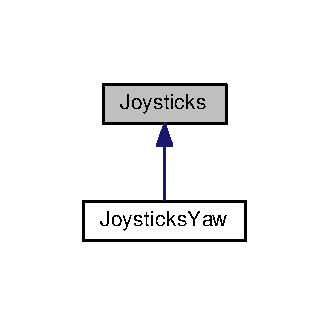
\includegraphics[width=158pt]{structJoysticks__inherit__graph}
\end{center}
\end{figure}
\subsection*{Public Member Functions}
\begin{DoxyCompactItemize}
\item 
\hyperlink{structJoysticks_a4326d4f2c4764a77b9f5c2e41aeae802}{Joysticks} ()
\begin{DoxyCompactList}\small\item\em Constructor that implicitly instantiates channels to zero. \end{DoxyCompactList}\item 
\hyperlink{structJoysticks_abe8777545ab8bbaa2282fa09e12041d9}{Joysticks} (double \hyperlink{structJoysticks_a3dc64d66808dddbf053033465777c493}{channel1}, double \hyperlink{structJoysticks_a14f4be76749f40ea8d75d579504ef932}{channel2}, double \hyperlink{structJoysticks_a2640f7dbb2364b8d92c464077c38ec56}{channel3}, double \hyperlink{structJoysticks_a154d66609cbfcb527d4dcf7473bf7af5}{channel4})
\begin{DoxyCompactList}\small\item\em Constructor that explicitly takes in states. \end{DoxyCompactList}\end{DoxyCompactItemize}
\subsection*{Public Attributes}
\begin{DoxyCompactItemize}
\item 
double \hyperlink{structJoysticks_a3dc64d66808dddbf053033465777c493}{channel1}
\begin{DoxyCompactList}\small\item\em First channel. \end{DoxyCompactList}\item 
double \hyperlink{structJoysticks_a14f4be76749f40ea8d75d579504ef932}{channel2}
\begin{DoxyCompactList}\small\item\em Second channel. \end{DoxyCompactList}\item 
double \hyperlink{structJoysticks_a2640f7dbb2364b8d92c464077c38ec56}{channel3}
\begin{DoxyCompactList}\small\item\em Third channel. \end{DoxyCompactList}\item 
double \hyperlink{structJoysticks_a154d66609cbfcb527d4dcf7473bf7af5}{channel4}
\begin{DoxyCompactList}\small\item\em Fourth channel. \end{DoxyCompactList}\end{DoxyCompactItemize}


\subsection{Detailed Description}
4channel Joystick data 

\subsection{Constructor \& Destructor Documentation}
\hypertarget{structJoysticks_a4326d4f2c4764a77b9f5c2e41aeae802}{\index{Joysticks@{Joysticks}!Joysticks@{Joysticks}}
\index{Joysticks@{Joysticks}!Joysticks@{Joysticks}}
\subsubsection[{Joysticks}]{\setlength{\rightskip}{0pt plus 5cm}Joysticks\-::\-Joysticks (
\begin{DoxyParamCaption}
{}
\end{DoxyParamCaption}
)\hspace{0.3cm}{\ttfamily [inline]}}}\label{structJoysticks_a4326d4f2c4764a77b9f5c2e41aeae802}


Constructor that implicitly instantiates channels to zero. 

\hypertarget{structJoysticks_abe8777545ab8bbaa2282fa09e12041d9}{\index{Joysticks@{Joysticks}!Joysticks@{Joysticks}}
\index{Joysticks@{Joysticks}!Joysticks@{Joysticks}}
\subsubsection[{Joysticks}]{\setlength{\rightskip}{0pt plus 5cm}Joysticks\-::\-Joysticks (
\begin{DoxyParamCaption}
\item[{double}]{channel1, }
\item[{double}]{channel2, }
\item[{double}]{channel3, }
\item[{double}]{channel4}
\end{DoxyParamCaption}
)\hspace{0.3cm}{\ttfamily [inline]}}}\label{structJoysticks_abe8777545ab8bbaa2282fa09e12041d9}


Constructor that explicitly takes in states. 


\begin{DoxyParams}{Parameters}
{\em channel1} & First channel \\
\hline
{\em channel2} & Second channel \\
\hline
{\em channel3} & Third channel \\
\hline
{\em channel4} & Fourth channel \\
\hline
\end{DoxyParams}


\subsection{Member Data Documentation}
\hypertarget{structJoysticks_a3dc64d66808dddbf053033465777c493}{\index{Joysticks@{Joysticks}!channel1@{channel1}}
\index{channel1@{channel1}!Joysticks@{Joysticks}}
\subsubsection[{channel1}]{\setlength{\rightskip}{0pt plus 5cm}double Joysticks\-::channel1}}\label{structJoysticks_a3dc64d66808dddbf053033465777c493}


First channel. 

\hypertarget{structJoysticks_a14f4be76749f40ea8d75d579504ef932}{\index{Joysticks@{Joysticks}!channel2@{channel2}}
\index{channel2@{channel2}!Joysticks@{Joysticks}}
\subsubsection[{channel2}]{\setlength{\rightskip}{0pt plus 5cm}double Joysticks\-::channel2}}\label{structJoysticks_a14f4be76749f40ea8d75d579504ef932}


Second channel. 

\hypertarget{structJoysticks_a2640f7dbb2364b8d92c464077c38ec56}{\index{Joysticks@{Joysticks}!channel3@{channel3}}
\index{channel3@{channel3}!Joysticks@{Joysticks}}
\subsubsection[{channel3}]{\setlength{\rightskip}{0pt plus 5cm}double Joysticks\-::channel3}}\label{structJoysticks_a2640f7dbb2364b8d92c464077c38ec56}


Third channel. 

\hypertarget{structJoysticks_a154d66609cbfcb527d4dcf7473bf7af5}{\index{Joysticks@{Joysticks}!channel4@{channel4}}
\index{channel4@{channel4}!Joysticks@{Joysticks}}
\subsubsection[{channel4}]{\setlength{\rightskip}{0pt plus 5cm}double Joysticks\-::channel4}}\label{structJoysticks_a154d66609cbfcb527d4dcf7473bf7af5}


Fourth channel. 



The documentation for this struct was generated from the following file\-:\begin{DoxyCompactItemize}
\item 
include/aerial\-\_\-autonomy/types/\hyperlink{joysticks_8h}{joysticks.\-h}\end{DoxyCompactItemize}

\hypertarget{structJoysticksYaw}{\section{Joysticks\-Yaw Struct Reference}
\label{structJoysticksYaw}\index{Joysticks\-Yaw@{Joysticks\-Yaw}}
}


Combined joystick and yaw data.  




{\ttfamily \#include $<$joysticks\-\_\-yaw.\-h$>$}



Inheritance diagram for Joysticks\-Yaw\-:\nopagebreak
\begin{figure}[H]
\begin{center}
\leavevmode
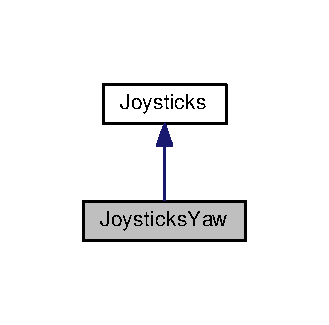
\includegraphics[width=158pt]{structJoysticksYaw__inherit__graph}
\end{center}
\end{figure}


Collaboration diagram for Joysticks\-Yaw\-:\nopagebreak
\begin{figure}[H]
\begin{center}
\leavevmode
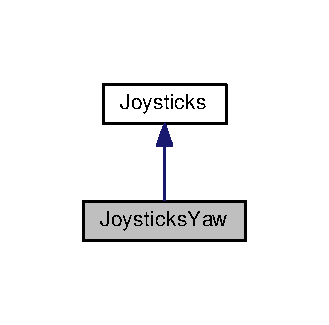
\includegraphics[width=158pt]{structJoysticksYaw__coll__graph}
\end{center}
\end{figure}
\subsection*{Public Member Functions}
\begin{DoxyCompactItemize}
\item 
\hyperlink{structJoysticksYaw_a1a5b1cf8d91d31c8aa7fb63acfc5833c}{Joysticks\-Yaw} ()
\begin{DoxyCompactList}\small\item\em constructor that takes implicitly instantiates joystick and yaw data \end{DoxyCompactList}\item 
\hyperlink{structJoysticksYaw_a01b433c411a2071821fded99f9f17a2b}{Joysticks\-Yaw} (double \hyperlink{structJoysticks_a3dc64d66808dddbf053033465777c493}{channel1}, double \hyperlink{structJoysticks_a14f4be76749f40ea8d75d579504ef932}{channel2}, double \hyperlink{structJoysticks_a2640f7dbb2364b8d92c464077c38ec56}{channel3}, double \hyperlink{structJoysticks_a154d66609cbfcb527d4dcf7473bf7af5}{channel4}, double \hyperlink{structJoysticksYaw_aed456b5f37609c1b68843ccf1e29019a}{yaw})
\begin{DoxyCompactList}\small\item\em Explicitly take in channel, yaw data. \end{DoxyCompactList}\end{DoxyCompactItemize}
\subsection*{Public Attributes}
\begin{DoxyCompactItemize}
\item 
double \hyperlink{structJoysticksYaw_aed456b5f37609c1b68843ccf1e29019a}{yaw}
\begin{DoxyCompactList}\small\item\em Yaw data stored internally. \end{DoxyCompactList}\end{DoxyCompactItemize}


\subsection{Detailed Description}
Combined joystick and yaw data. 

\subsection{Constructor \& Destructor Documentation}
\hypertarget{structJoysticksYaw_a1a5b1cf8d91d31c8aa7fb63acfc5833c}{\index{Joysticks\-Yaw@{Joysticks\-Yaw}!Joysticks\-Yaw@{Joysticks\-Yaw}}
\index{Joysticks\-Yaw@{Joysticks\-Yaw}!JoysticksYaw@{Joysticks\-Yaw}}
\subsubsection[{Joysticks\-Yaw}]{\setlength{\rightskip}{0pt plus 5cm}Joysticks\-Yaw\-::\-Joysticks\-Yaw (
\begin{DoxyParamCaption}
{}
\end{DoxyParamCaption}
)\hspace{0.3cm}{\ttfamily [inline]}}}\label{structJoysticksYaw_a1a5b1cf8d91d31c8aa7fb63acfc5833c}


constructor that takes implicitly instantiates joystick and yaw data 

\hypertarget{structJoysticksYaw_a01b433c411a2071821fded99f9f17a2b}{\index{Joysticks\-Yaw@{Joysticks\-Yaw}!Joysticks\-Yaw@{Joysticks\-Yaw}}
\index{Joysticks\-Yaw@{Joysticks\-Yaw}!JoysticksYaw@{Joysticks\-Yaw}}
\subsubsection[{Joysticks\-Yaw}]{\setlength{\rightskip}{0pt plus 5cm}Joysticks\-Yaw\-::\-Joysticks\-Yaw (
\begin{DoxyParamCaption}
\item[{double}]{channel1, }
\item[{double}]{channel2, }
\item[{double}]{channel3, }
\item[{double}]{channel4, }
\item[{double}]{yaw}
\end{DoxyParamCaption}
)\hspace{0.3cm}{\ttfamily [inline]}}}\label{structJoysticksYaw_a01b433c411a2071821fded99f9f17a2b}


Explicitly take in channel, yaw data. 


\begin{DoxyParams}{Parameters}
{\em channel1} & First Channel \\
\hline
{\em channel2} & Second Channel \\
\hline
{\em channel3} & Third Channel \\
\hline
{\em channel4} & Fourth Channel \\
\hline
{\em yaw} & Yaw data \\
\hline
\end{DoxyParams}


\subsection{Member Data Documentation}
\hypertarget{structJoysticksYaw_aed456b5f37609c1b68843ccf1e29019a}{\index{Joysticks\-Yaw@{Joysticks\-Yaw}!yaw@{yaw}}
\index{yaw@{yaw}!JoysticksYaw@{Joysticks\-Yaw}}
\subsubsection[{yaw}]{\setlength{\rightskip}{0pt plus 5cm}double Joysticks\-Yaw\-::yaw}}\label{structJoysticksYaw_aed456b5f37609c1b68843ccf1e29019a}


Yaw data stored internally. 



The documentation for this struct was generated from the following file\-:\begin{DoxyCompactItemize}
\item 
include/aerial\-\_\-autonomy/types/\hyperlink{joysticks__yaw_8h}{joysticks\-\_\-yaw.\-h}\end{DoxyCompactItemize}

\hypertarget{structLogicStateMachineFrontEnd_1_1Landed}{\section{Logic\-State\-Machine\-Front\-End\-:\-:Landed Struct Reference}
\label{structLogicStateMachineFrontEnd_1_1Landed}\index{Logic\-State\-Machine\-Front\-End\-::\-Landed@{Logic\-State\-Machine\-Front\-End\-::\-Landed}}
}


\hyperlink{structLogicStateMachineFrontEnd_1_1Landed}{Landed} state.  




{\ttfamily \#include $<$basic\-\_\-state\-\_\-machine.\-h$>$}



Inheritance diagram for Logic\-State\-Machine\-Front\-End\-:\-:Landed\-:\nopagebreak
\begin{figure}[H]
\begin{center}
\leavevmode
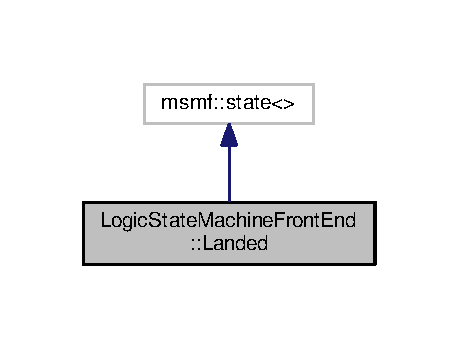
\includegraphics[width=220pt]{structLogicStateMachineFrontEnd_1_1Landed__inherit__graph}
\end{center}
\end{figure}


Collaboration diagram for Logic\-State\-Machine\-Front\-End\-:\-:Landed\-:\nopagebreak
\begin{figure}[H]
\begin{center}
\leavevmode
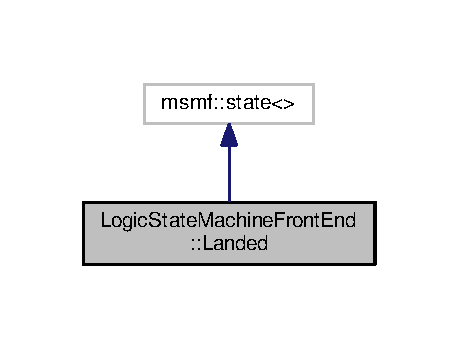
\includegraphics[width=220pt]{structLogicStateMachineFrontEnd_1_1Landed__coll__graph}
\end{center}
\end{figure}
\subsection*{Classes}
\begin{DoxyCompactItemize}
\item 
struct \hyperlink{structLogicStateMachineFrontEnd_1_1Landed_1_1internal__transition__table}{internal\-\_\-transition\-\_\-table}
\begin{DoxyCompactList}\small\item\em Internal event without any action. \end{DoxyCompactList}\end{DoxyCompactItemize}


\subsection{Detailed Description}
\hyperlink{structLogicStateMachineFrontEnd_1_1Landed}{Landed} state. 

The documentation for this struct was generated from the following file\-:\begin{DoxyCompactItemize}
\item 
include/aerial\-\_\-autonomy/state\-\_\-machines/\hyperlink{basic__state__machine_8h}{basic\-\_\-state\-\_\-machine.\-h}\end{DoxyCompactItemize}

\hypertarget{structLandInternalActionFunctor__}{\section{Land\-Internal\-Action\-Functor\-\_\-$<$ Logic\-State\-Machine\-T $>$ Struct Template Reference}
\label{structLandInternalActionFunctor__}\index{Land\-Internal\-Action\-Functor\-\_\-$<$ Logic\-State\-Machine\-T $>$@{Land\-Internal\-Action\-Functor\-\_\-$<$ Logic\-State\-Machine\-T $>$}}
}


Internal action to figure out when landing is complete.  




{\ttfamily \#include $<$land\-\_\-functors.\-h$>$}



Inheritance diagram for Land\-Internal\-Action\-Functor\-\_\-$<$ Logic\-State\-Machine\-T $>$\-:\nopagebreak
\begin{figure}[H]
\begin{center}
\leavevmode
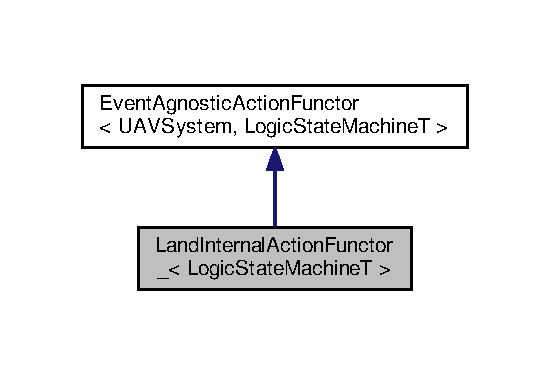
\includegraphics[width=264pt]{structLandInternalActionFunctor____inherit__graph}
\end{center}
\end{figure}


Collaboration diagram for Land\-Internal\-Action\-Functor\-\_\-$<$ Logic\-State\-Machine\-T $>$\-:\nopagebreak
\begin{figure}[H]
\begin{center}
\leavevmode
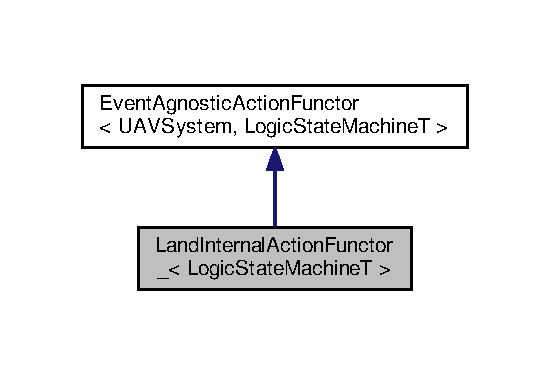
\includegraphics[width=264pt]{structLandInternalActionFunctor____coll__graph}
\end{center}
\end{figure}
\subsection*{Public Member Functions}
\begin{DoxyCompactItemize}
\item 
void \hyperlink{structLandInternalActionFunctor___a4557b02d6cfa6712b610337cb606f54b}{run} (\hyperlink{classUAVSystem}{U\-A\-V\-System} \&robot\-\_\-system, Logic\-State\-Machine\-T \&logic\-\_\-state\-\_\-machine)
\begin{DoxyCompactList}\small\item\em Internal function to check when landing is complete. \end{DoxyCompactList}\end{DoxyCompactItemize}


\subsection{Detailed Description}
\subsubsection*{template$<$class Logic\-State\-Machine\-T$>$struct Land\-Internal\-Action\-Functor\-\_\-$<$ Logic\-State\-Machine\-T $>$}

Internal action to figure out when landing is complete. 

\begin{DoxyRefDesc}{Todo}
\item[\hyperlink{todo__todo000006}{Todo}](Gowtham) How to abort Land??\end{DoxyRefDesc}



\begin{DoxyTemplParams}{Template Parameters}
{\em Logic\-State\-Machine\-T} & Logic state machine used to process events \\
\hline
\end{DoxyTemplParams}


\subsection{Member Function Documentation}
\hypertarget{structLandInternalActionFunctor___a4557b02d6cfa6712b610337cb606f54b}{\index{Land\-Internal\-Action\-Functor\-\_\-@{Land\-Internal\-Action\-Functor\-\_\-}!run@{run}}
\index{run@{run}!LandInternalActionFunctor_@{Land\-Internal\-Action\-Functor\-\_\-}}
\subsubsection[{run}]{\setlength{\rightskip}{0pt plus 5cm}template$<$class Logic\-State\-Machine\-T $>$ void {\bf Land\-Internal\-Action\-Functor\-\_\-}$<$ Logic\-State\-Machine\-T $>$\-::run (
\begin{DoxyParamCaption}
\item[{{\bf U\-A\-V\-System} \&}]{robot\-\_\-system, }
\item[{Logic\-State\-Machine\-T \&}]{logic\-\_\-state\-\_\-machine}
\end{DoxyParamCaption}
)\hspace{0.3cm}{\ttfamily [inline]}, {\ttfamily [virtual]}}}\label{structLandInternalActionFunctor___a4557b02d6cfa6712b610337cb606f54b}


Internal function to check when landing is complete. 


\begin{DoxyParams}{Parameters}
{\em robot\-\_\-system} & robot system to get sensor data \\
\hline
{\em logic\-\_\-state\-\_\-machine} & logic state machine to trigger events \\
\hline
\end{DoxyParams}
\begin{DoxyRefDesc}{Todo}
\item[\hyperlink{todo__todo000008}{Todo}](Gowtham) Can also use uav status here \end{DoxyRefDesc}


Implements \hyperlink{structEventAgnosticActionFunctor_a53a48938d68370ff2ef262222565ffcf}{Event\-Agnostic\-Action\-Functor$<$ U\-A\-V\-System, Logic\-State\-Machine\-T $>$}.



The documentation for this struct was generated from the following file\-:\begin{DoxyCompactItemize}
\item 
include/aerial\-\_\-autonomy/actions\-\_\-guards/\hyperlink{land__functors_8h}{land\-\_\-functors.\-h}\end{DoxyCompactItemize}

\hypertarget{structLandTransitionActionFunctor__}{\section{Land\-Transition\-Action\-Functor\-\_\-$<$ Logic\-State\-Machine\-T $>$ Struct Template Reference}
\label{structLandTransitionActionFunctor__}\index{Land\-Transition\-Action\-Functor\-\_\-$<$ Logic\-State\-Machine\-T $>$@{Land\-Transition\-Action\-Functor\-\_\-$<$ Logic\-State\-Machine\-T $>$}}
}


Transition action when starting to land.  




{\ttfamily \#include $<$land\-\_\-functors.\-h$>$}



Inheritance diagram for Land\-Transition\-Action\-Functor\-\_\-$<$ Logic\-State\-Machine\-T $>$\-:\nopagebreak
\begin{figure}[H]
\begin{center}
\leavevmode
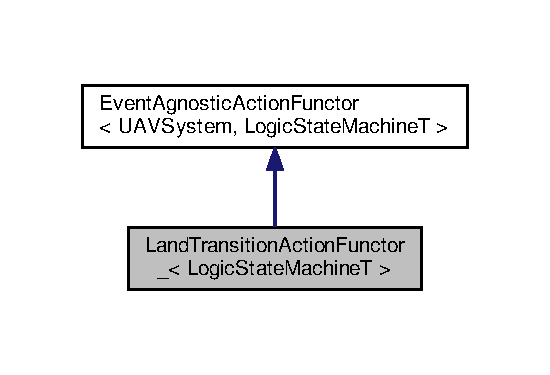
\includegraphics[width=264pt]{structLandTransitionActionFunctor____inherit__graph}
\end{center}
\end{figure}


Collaboration diagram for Land\-Transition\-Action\-Functor\-\_\-$<$ Logic\-State\-Machine\-T $>$\-:\nopagebreak
\begin{figure}[H]
\begin{center}
\leavevmode
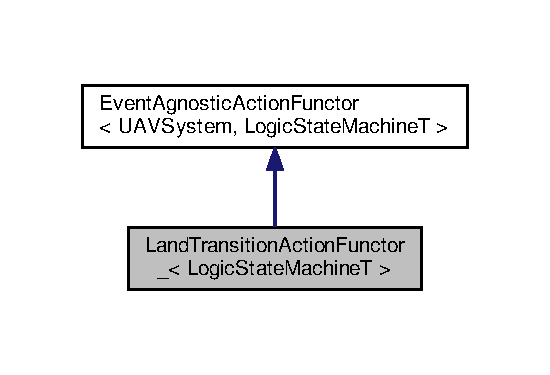
\includegraphics[width=264pt]{structLandTransitionActionFunctor____coll__graph}
\end{center}
\end{figure}
\subsection*{Public Member Functions}
\begin{DoxyCompactItemize}
\item 
void \hyperlink{structLandTransitionActionFunctor___ae91b354f041edda283e306fa312e1213}{run} (\hyperlink{classUAVSystem}{U\-A\-V\-System} \&robot\-\_\-system, Logic\-State\-Machine\-T \&)
\begin{DoxyCompactList}\small\item\em Override this run function for different sub classes. This function performs the logic checking for each state. \end{DoxyCompactList}\end{DoxyCompactItemize}


\subsection{Detailed Description}
\subsubsection*{template$<$class Logic\-State\-Machine\-T$>$struct Land\-Transition\-Action\-Functor\-\_\-$<$ Logic\-State\-Machine\-T $>$}

Transition action when starting to land. 


\begin{DoxyTemplParams}{Template Parameters}
{\em Logic\-State\-Machine\-T} & Logic state machine used to process events \\
\hline
\end{DoxyTemplParams}


\subsection{Member Function Documentation}
\hypertarget{structLandTransitionActionFunctor___ae91b354f041edda283e306fa312e1213}{\index{Land\-Transition\-Action\-Functor\-\_\-@{Land\-Transition\-Action\-Functor\-\_\-}!run@{run}}
\index{run@{run}!LandTransitionActionFunctor_@{Land\-Transition\-Action\-Functor\-\_\-}}
\subsubsection[{run}]{\setlength{\rightskip}{0pt plus 5cm}template$<$class Logic\-State\-Machine\-T $>$ void {\bf Land\-Transition\-Action\-Functor\-\_\-}$<$ Logic\-State\-Machine\-T $>$\-::run (
\begin{DoxyParamCaption}
\item[{{\bf U\-A\-V\-System} \&}]{robot\-\_\-system, }
\item[{Logic\-State\-Machine\-T \&}]{logic\-\_\-state\-\_\-machine}
\end{DoxyParamCaption}
)\hspace{0.3cm}{\ttfamily [inline]}, {\ttfamily [virtual]}}}\label{structLandTransitionActionFunctor___ae91b354f041edda283e306fa312e1213}


Override this run function for different sub classes. This function performs the logic checking for each state. 


\begin{DoxyParams}{Parameters}
{\em robot\-\_\-system} & Provides sensor data and allows for controlling hardware \\
\hline
{\em logic\-\_\-state\-\_\-machine} & Backend of logic State Machine. can send events using this. \\
\hline
\end{DoxyParams}
\begin{DoxyRefDesc}{Todo}
\item[\hyperlink{todo__todo000007}{Todo}]Have to abort all hardware controllers not just U\-A\-V. \end{DoxyRefDesc}


Implements \hyperlink{structEventAgnosticActionFunctor_a53a48938d68370ff2ef262222565ffcf}{Event\-Agnostic\-Action\-Functor$<$ U\-A\-V\-System, Logic\-State\-Machine\-T $>$}.



The documentation for this struct was generated from the following file\-:\begin{DoxyCompactItemize}
\item 
include/aerial\-\_\-autonomy/actions\-\_\-guards/\hyperlink{land__functors_8h}{land\-\_\-functors.\-h}\end{DoxyCompactItemize}

\hypertarget{classLogicStateMachineFrontEnd}{\section{Logic\-State\-Machine\-Front\-End Class Reference}
\label{classLogicStateMachineFrontEnd}\index{Logic\-State\-Machine\-Front\-End@{Logic\-State\-Machine\-Front\-End}}
}


front-\/end\-: define the F\-S\-M structure  




{\ttfamily \#include $<$basic\-\_\-state\-\_\-machine.\-h$>$}



Inheritance diagram for Logic\-State\-Machine\-Front\-End\-:\nopagebreak
\begin{figure}[H]
\begin{center}
\leavevmode
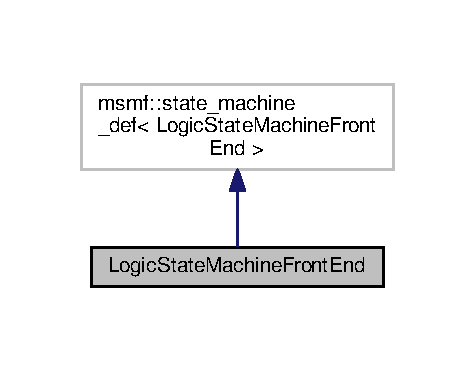
\includegraphics[width=228pt]{classLogicStateMachineFrontEnd__inherit__graph}
\end{center}
\end{figure}


Collaboration diagram for Logic\-State\-Machine\-Front\-End\-:\nopagebreak
\begin{figure}[H]
\begin{center}
\leavevmode
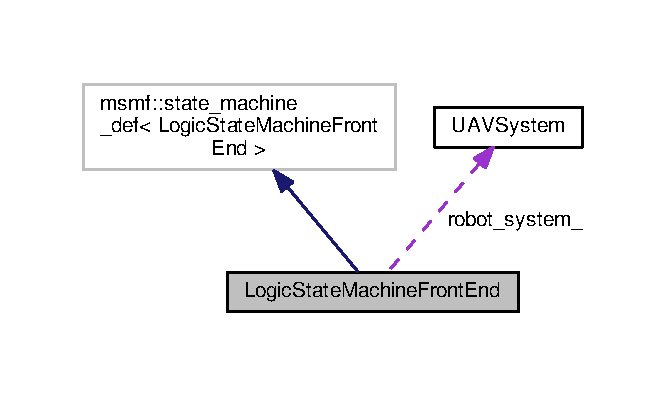
\includegraphics[width=320pt]{classLogicStateMachineFrontEnd__coll__graph}
\end{center}
\end{figure}
\subsection*{Classes}
\begin{DoxyCompactItemize}
\item 
struct \hyperlink{structLogicStateMachineFrontEnd_1_1Landed}{Landed}
\begin{DoxyCompactList}\small\item\em \hyperlink{structLogicStateMachineFrontEnd_1_1Landed}{Landed} state. \end{DoxyCompactList}\item 
struct \hyperlink{structLogicStateMachineFrontEnd_1_1transition__table}{transition\-\_\-table}
\begin{DoxyCompactList}\small\item\em Transition table for State Machine. \end{DoxyCompactList}\end{DoxyCompactItemize}
\subsection*{Public Types}
\begin{DoxyCompactItemize}
\item 
using \hyperlink{classLogicStateMachineFrontEnd_a98f3148dbabd87749be3c63ea0ec2a00}{Taking\-Off} = \hyperlink{takeoff__functors_8h_ab6710f3cb12b7653eedcd3a2215d3228}{Taking\-Off\-\_\-}$<$ \hyperlink{basic__state__machine_8h_ab0b6ef21baf57684550a2f05c771bd86}{Logic\-State\-Machine} $>$
\begin{DoxyCompactList}\small\item\em Takingoff state. \end{DoxyCompactList}\item 
using \hyperlink{classLogicStateMachineFrontEnd_acac7938fd313e8808e486fa884ccf49b}{Landing} = \hyperlink{land__functors_8h_a84627965433a60de431758bddec005c3}{Landing\-\_\-}$<$ \hyperlink{basic__state__machine_8h_ab0b6ef21baf57684550a2f05c771bd86}{Logic\-State\-Machine} $>$
\begin{DoxyCompactList}\small\item\em Landing state. \end{DoxyCompactList}\item 
using \hyperlink{classLogicStateMachineFrontEnd_a8a5e85c9d100560fc79f9cbe1bbd5947}{Reaching\-Goal} = \hyperlink{position__control__functors_8h_af380346c24b534da18813f70217ea50f}{Reaching\-Goal\-\_\-}$<$ \hyperlink{basic__state__machine_8h_ab0b6ef21baf57684550a2f05c771bd86}{Logic\-State\-Machine} $>$
\begin{DoxyCompactList}\small\item\em Reaching goal state. \end{DoxyCompactList}\item 
using \hyperlink{classLogicStateMachineFrontEnd_a5877b5b19ba413c2b3bb02ee2459d5ec}{Hovering} = \hyperlink{hovering__functors_8h_a4252f403b3bcd2a850cf271512d9c6ff}{Hovering\-\_\-}$<$ \hyperlink{basic__state__machine_8h_ab0b6ef21baf57684550a2f05c771bd86}{Logic\-State\-Machine} $>$
\begin{DoxyCompactList}\small\item\em Hovering state. \end{DoxyCompactList}\item 
using \hyperlink{classLogicStateMachineFrontEnd_ae617089cdb6687edc5d27b7f8a546af2}{initial\-\_\-state} = \hyperlink{structLogicStateMachineFrontEnd_1_1Landed}{Landed}
\begin{DoxyCompactList}\small\item\em Initial state for state machine. \end{DoxyCompactList}\item 
using \hyperlink{classLogicStateMachineFrontEnd_af73bbbe19d413f3786c265fe91a94ffb}{Takeoff\-Action} = \hyperlink{structTakeoffTransitionActionFunctor__}{Takeoff\-Transition\-Action\-Functor\-\_\-}$<$ \hyperlink{basic__state__machine_8h_ab0b6ef21baf57684550a2f05c771bd86}{Logic\-State\-Machine} $>$
\begin{DoxyCompactList}\small\item\em Action to take when taking off. \end{DoxyCompactList}\item 
using \hyperlink{classLogicStateMachineFrontEnd_a4660e7e7dbd8bc3f7a379a076999187d}{Takeoff\-Guard} = \hyperlink{structTakeoffTransitionGuardFunctor__}{Takeoff\-Transition\-Guard\-Functor\-\_\-}$<$ \hyperlink{basic__state__machine_8h_ab0b6ef21baf57684550a2f05c771bd86}{Logic\-State\-Machine} $>$
\begin{DoxyCompactList}\small\item\em Guard to stop taking off under low voltage. \end{DoxyCompactList}\item 
using \hyperlink{classLogicStateMachineFrontEnd_a26036773cac59b48b9e545acc870a29b}{Takeoff\-Abort} = \hyperlink{structTakeoffAbortActionFunctor__}{Takeoff\-Abort\-Action\-Functor\-\_\-}$<$ \hyperlink{basic__state__machine_8h_ab0b6ef21baf57684550a2f05c771bd86}{Logic\-State\-Machine} $>$
\begin{DoxyCompactList}\small\item\em Abort action when taking off. \end{DoxyCompactList}\item 
using \hyperlink{classLogicStateMachineFrontEnd_ad1619c7d43a216eb9238004470389f2e}{Landing\-Action} = \hyperlink{structLandTransitionActionFunctor__}{Land\-Transition\-Action\-Functor\-\_\-}$<$ \hyperlink{basic__state__machine_8h_ab0b6ef21baf57684550a2f05c771bd86}{Logic\-State\-Machine} $>$
\begin{DoxyCompactList}\small\item\em Action to take when landing. \end{DoxyCompactList}\item 
using \hyperlink{classLogicStateMachineFrontEnd_a39babee29ba680422ea922504a465417}{Reaching\-Goal\-Set} = \hyperlink{structPositionControlTransitionActionFunctor__}{Position\-Control\-Transition\-Action\-Functor\-\_\-}$<$ \hyperlink{basic__state__machine_8h_ab0b6ef21baf57684550a2f05c771bd86}{Logic\-State\-Machine} $>$
\begin{DoxyCompactList}\small\item\em set goal action when transitioning \end{DoxyCompactList}\item 
using \hyperlink{classLogicStateMachineFrontEnd_a84fe5b03b104adc3c3406bb0b6ffa190}{Reaching\-Goal\-Guard} = \hyperlink{structPositionControlTransitionGuardFunctor__}{Position\-Control\-Transition\-Guard\-Functor\-\_\-}$<$ \hyperlink{basic__state__machine_8h_ab0b6ef21baf57684550a2f05c771bd86}{Logic\-State\-Machine} $>$
\begin{DoxyCompactList}\small\item\em Guard to avoid going to goal if goal is not correct. \end{DoxyCompactList}\item 
using \hyperlink{classLogicStateMachineFrontEnd_a6273a06430b7aa6088e25d9b78805f1a}{Reaching\-Goal\-Abort} = \hyperlink{structPositionControlAbortActionFunctor__}{Position\-Control\-Abort\-Action\-Functor\-\_\-}$<$ \hyperlink{basic__state__machine_8h_ab0b6ef21baf57684550a2f05c771bd86}{Logic\-State\-Machine} $>$
\begin{DoxyCompactList}\small\item\em Abort action when reaching goal. \end{DoxyCompactList}\item 
using \hyperlink{classLogicStateMachineFrontEnd_a3bec78d997dbc5ae5534c3b49c8127f5}{Reaching\-Goal\-Land} = \hyperlink{classLogicStateMachineFrontEnd_ad1619c7d43a216eb9238004470389f2e}{Landing\-Action}
\begin{DoxyCompactList}\small\item\em Land action when reaching goal. \end{DoxyCompactList}\end{DoxyCompactItemize}
\subsection*{Public Member Functions}
\begin{DoxyCompactItemize}
\item 
std\-::type\-\_\-index \hyperlink{classLogicStateMachineFrontEnd_af2ccbab79c14bc6570091b49a2e61fff}{get\-\_\-no\-\_\-transition\-\_\-event\-\_\-index} ()
\begin{DoxyCompactList}\small\item\em Returns the index of the event that did not trigger any transition. \end{DoxyCompactList}\item 
{\footnotesize template$<$class Event , class F\-S\-M $>$ }\\void \hyperlink{classLogicStateMachineFrontEnd_afea624ef452f4dd6f5380c96fd9555bb}{on\-\_\-entry} (Event const \&, F\-S\-M \&)
\begin{DoxyCompactList}\small\item\em Action to take on entering state machine. \end{DoxyCompactList}\item 
{\footnotesize template$<$class Event , class F\-S\-M $>$ }\\void \hyperlink{classLogicStateMachineFrontEnd_a86bc9dc7c6ab97285bb5c9ea06517da3}{on\-\_\-exit} (Event const \&, F\-S\-M \&)
\begin{DoxyCompactList}\small\item\em Action to take on leaving state machine. \end{DoxyCompactList}\item 
\hyperlink{classLogicStateMachineFrontEnd_a38a4d9fba9466fa36d012d297e8908ec}{Logic\-State\-Machine\-Front\-End} (\hyperlink{classUAVSystem}{U\-A\-V\-System} \&uav\-\_\-system)
\begin{DoxyCompactList}\small\item\em Constructor with arguments to store robot system. \end{DoxyCompactList}\item 
{\footnotesize template$<$class F\-S\-M , class Event $>$ }\\void \hyperlink{classLogicStateMachineFrontEnd_aa75b2a1500d4bfe052c5421aeefbf7ab}{no\-\_\-transition} (Event const \&e, F\-S\-M \&, int state\-\_\-index)
\begin{DoxyCompactList}\small\item\em Print event typeid if no action present for the corresponding event. \end{DoxyCompactList}\end{DoxyCompactItemize}
\subsection*{Protected Attributes}
\begin{DoxyCompactItemize}
\item 
\hyperlink{classUAVSystem}{U\-A\-V\-System} \& \hyperlink{classLogicStateMachineFrontEnd_a8431e5208e24b80105d639281361a252}{robot\-\_\-system\-\_\-}
\begin{DoxyCompactList}\small\item\em robot system used by states to get sensor data and send commands \end{DoxyCompactList}\item 
std\-::type\-\_\-index \hyperlink{classLogicStateMachineFrontEnd_a0f19247a261344e58dede909f598677f}{no\-\_\-transition\-\_\-event\-\_\-index\-\_\-} = typeid(N\-U\-L\-L)
\begin{DoxyCompactList}\small\item\em type index to store the event that did not trigger any transition \end{DoxyCompactList}\end{DoxyCompactItemize}
\subsection*{Friends}
\begin{DoxyCompactItemize}
\item 
{\footnotesize template$<$class Event\-T , class Robot\-System\-T , class Logic\-State\-Machine\-T $>$ }\\class \hyperlink{classLogicStateMachineFrontEnd_a05673eb4ec343f36c1f3fb787ac26b94}{Action\-Functor}
\item 
{\footnotesize template$<$class Event\-T , class Robot\-System\-T , class Logic\-State\-Machine\-T $>$ }\\class \hyperlink{classLogicStateMachineFrontEnd_a9411581bb37b54467df520e3c73ceaf0}{Guard\-Functor}
\item 
{\footnotesize template$<$class Robot\-System\-T1 , class Logic\-State\-Machine\-T $>$ }\\class \hyperlink{classLogicStateMachineFrontEnd_a86a665e36420c3cbc2b45864e023f98a}{Event\-Agnostic\-Action\-Functor}
\item 
{\footnotesize template$<$class Robot\-System\-T1 , class Logic\-State\-Machine\-T $>$ }\\class \hyperlink{classLogicStateMachineFrontEnd_af372c36475bc4510af791f5cb66608ad}{Event\-Agnostic\-Guard\-Functor}
\end{DoxyCompactItemize}


\subsection{Detailed Description}
front-\/end\-: define the F\-S\-M structure 

\subsection{Member Typedef Documentation}
\hypertarget{classLogicStateMachineFrontEnd_a5877b5b19ba413c2b3bb02ee2459d5ec}{\index{Logic\-State\-Machine\-Front\-End@{Logic\-State\-Machine\-Front\-End}!Hovering@{Hovering}}
\index{Hovering@{Hovering}!LogicStateMachineFrontEnd@{Logic\-State\-Machine\-Front\-End}}
\subsubsection[{Hovering}]{\setlength{\rightskip}{0pt plus 5cm}using {\bf Logic\-State\-Machine\-Front\-End\-::\-Hovering} =  {\bf Hovering\-\_\-}$<${\bf Logic\-State\-Machine}$>$}}\label{classLogicStateMachineFrontEnd_a5877b5b19ba413c2b3bb02ee2459d5ec}


Hovering state. 

\hypertarget{classLogicStateMachineFrontEnd_ae617089cdb6687edc5d27b7f8a546af2}{\index{Logic\-State\-Machine\-Front\-End@{Logic\-State\-Machine\-Front\-End}!initial\-\_\-state@{initial\-\_\-state}}
\index{initial\-\_\-state@{initial\-\_\-state}!LogicStateMachineFrontEnd@{Logic\-State\-Machine\-Front\-End}}
\subsubsection[{initial\-\_\-state}]{\setlength{\rightskip}{0pt plus 5cm}using {\bf Logic\-State\-Machine\-Front\-End\-::initial\-\_\-state} =  {\bf Landed}}}\label{classLogicStateMachineFrontEnd_ae617089cdb6687edc5d27b7f8a546af2}


Initial state for state machine. 

\hypertarget{classLogicStateMachineFrontEnd_acac7938fd313e8808e486fa884ccf49b}{\index{Logic\-State\-Machine\-Front\-End@{Logic\-State\-Machine\-Front\-End}!Landing@{Landing}}
\index{Landing@{Landing}!LogicStateMachineFrontEnd@{Logic\-State\-Machine\-Front\-End}}
\subsubsection[{Landing}]{\setlength{\rightskip}{0pt plus 5cm}using {\bf Logic\-State\-Machine\-Front\-End\-::\-Landing} =  {\bf Landing\-\_\-}$<${\bf Logic\-State\-Machine}$>$}}\label{classLogicStateMachineFrontEnd_acac7938fd313e8808e486fa884ccf49b}


Landing state. 

\hypertarget{classLogicStateMachineFrontEnd_ad1619c7d43a216eb9238004470389f2e}{\index{Logic\-State\-Machine\-Front\-End@{Logic\-State\-Machine\-Front\-End}!Landing\-Action@{Landing\-Action}}
\index{Landing\-Action@{Landing\-Action}!LogicStateMachineFrontEnd@{Logic\-State\-Machine\-Front\-End}}
\subsubsection[{Landing\-Action}]{\setlength{\rightskip}{0pt plus 5cm}using {\bf Logic\-State\-Machine\-Front\-End\-::\-Landing\-Action} =  {\bf Land\-Transition\-Action\-Functor\-\_\-}$<${\bf Logic\-State\-Machine}$>$}}\label{classLogicStateMachineFrontEnd_ad1619c7d43a216eb9238004470389f2e}


Action to take when landing. 

\hypertarget{classLogicStateMachineFrontEnd_a8a5e85c9d100560fc79f9cbe1bbd5947}{\index{Logic\-State\-Machine\-Front\-End@{Logic\-State\-Machine\-Front\-End}!Reaching\-Goal@{Reaching\-Goal}}
\index{Reaching\-Goal@{Reaching\-Goal}!LogicStateMachineFrontEnd@{Logic\-State\-Machine\-Front\-End}}
\subsubsection[{Reaching\-Goal}]{\setlength{\rightskip}{0pt plus 5cm}using {\bf Logic\-State\-Machine\-Front\-End\-::\-Reaching\-Goal} =  {\bf Reaching\-Goal\-\_\-}$<${\bf Logic\-State\-Machine}$>$}}\label{classLogicStateMachineFrontEnd_a8a5e85c9d100560fc79f9cbe1bbd5947}


Reaching goal state. 

\hypertarget{classLogicStateMachineFrontEnd_a6273a06430b7aa6088e25d9b78805f1a}{\index{Logic\-State\-Machine\-Front\-End@{Logic\-State\-Machine\-Front\-End}!Reaching\-Goal\-Abort@{Reaching\-Goal\-Abort}}
\index{Reaching\-Goal\-Abort@{Reaching\-Goal\-Abort}!LogicStateMachineFrontEnd@{Logic\-State\-Machine\-Front\-End}}
\subsubsection[{Reaching\-Goal\-Abort}]{\setlength{\rightskip}{0pt plus 5cm}using {\bf Logic\-State\-Machine\-Front\-End\-::\-Reaching\-Goal\-Abort} =  {\bf Position\-Control\-Abort\-Action\-Functor\-\_\-}$<${\bf Logic\-State\-Machine}$>$}}\label{classLogicStateMachineFrontEnd_a6273a06430b7aa6088e25d9b78805f1a}


Abort action when reaching goal. 

\hypertarget{classLogicStateMachineFrontEnd_a84fe5b03b104adc3c3406bb0b6ffa190}{\index{Logic\-State\-Machine\-Front\-End@{Logic\-State\-Machine\-Front\-End}!Reaching\-Goal\-Guard@{Reaching\-Goal\-Guard}}
\index{Reaching\-Goal\-Guard@{Reaching\-Goal\-Guard}!LogicStateMachineFrontEnd@{Logic\-State\-Machine\-Front\-End}}
\subsubsection[{Reaching\-Goal\-Guard}]{\setlength{\rightskip}{0pt plus 5cm}using {\bf Logic\-State\-Machine\-Front\-End\-::\-Reaching\-Goal\-Guard} =  {\bf Position\-Control\-Transition\-Guard\-Functor\-\_\-}$<${\bf Logic\-State\-Machine}$>$}}\label{classLogicStateMachineFrontEnd_a84fe5b03b104adc3c3406bb0b6ffa190}


Guard to avoid going to goal if goal is not correct. 

\hypertarget{classLogicStateMachineFrontEnd_a3bec78d997dbc5ae5534c3b49c8127f5}{\index{Logic\-State\-Machine\-Front\-End@{Logic\-State\-Machine\-Front\-End}!Reaching\-Goal\-Land@{Reaching\-Goal\-Land}}
\index{Reaching\-Goal\-Land@{Reaching\-Goal\-Land}!LogicStateMachineFrontEnd@{Logic\-State\-Machine\-Front\-End}}
\subsubsection[{Reaching\-Goal\-Land}]{\setlength{\rightskip}{0pt plus 5cm}using {\bf Logic\-State\-Machine\-Front\-End\-::\-Reaching\-Goal\-Land} =  {\bf Landing\-Action}}}\label{classLogicStateMachineFrontEnd_a3bec78d997dbc5ae5534c3b49c8127f5}


Land action when reaching goal. 

\hypertarget{classLogicStateMachineFrontEnd_a39babee29ba680422ea922504a465417}{\index{Logic\-State\-Machine\-Front\-End@{Logic\-State\-Machine\-Front\-End}!Reaching\-Goal\-Set@{Reaching\-Goal\-Set}}
\index{Reaching\-Goal\-Set@{Reaching\-Goal\-Set}!LogicStateMachineFrontEnd@{Logic\-State\-Machine\-Front\-End}}
\subsubsection[{Reaching\-Goal\-Set}]{\setlength{\rightskip}{0pt plus 5cm}using {\bf Logic\-State\-Machine\-Front\-End\-::\-Reaching\-Goal\-Set} =  {\bf Position\-Control\-Transition\-Action\-Functor\-\_\-}$<${\bf Logic\-State\-Machine}$>$}}\label{classLogicStateMachineFrontEnd_a39babee29ba680422ea922504a465417}


set goal action when transitioning 

\hypertarget{classLogicStateMachineFrontEnd_a26036773cac59b48b9e545acc870a29b}{\index{Logic\-State\-Machine\-Front\-End@{Logic\-State\-Machine\-Front\-End}!Takeoff\-Abort@{Takeoff\-Abort}}
\index{Takeoff\-Abort@{Takeoff\-Abort}!LogicStateMachineFrontEnd@{Logic\-State\-Machine\-Front\-End}}
\subsubsection[{Takeoff\-Abort}]{\setlength{\rightskip}{0pt plus 5cm}using {\bf Logic\-State\-Machine\-Front\-End\-::\-Takeoff\-Abort} =  {\bf Takeoff\-Abort\-Action\-Functor\-\_\-}$<${\bf Logic\-State\-Machine}$>$}}\label{classLogicStateMachineFrontEnd_a26036773cac59b48b9e545acc870a29b}


Abort action when taking off. 

\hypertarget{classLogicStateMachineFrontEnd_af73bbbe19d413f3786c265fe91a94ffb}{\index{Logic\-State\-Machine\-Front\-End@{Logic\-State\-Machine\-Front\-End}!Takeoff\-Action@{Takeoff\-Action}}
\index{Takeoff\-Action@{Takeoff\-Action}!LogicStateMachineFrontEnd@{Logic\-State\-Machine\-Front\-End}}
\subsubsection[{Takeoff\-Action}]{\setlength{\rightskip}{0pt plus 5cm}using {\bf Logic\-State\-Machine\-Front\-End\-::\-Takeoff\-Action} =  {\bf Takeoff\-Transition\-Action\-Functor\-\_\-}$<${\bf Logic\-State\-Machine}$>$}}\label{classLogicStateMachineFrontEnd_af73bbbe19d413f3786c265fe91a94ffb}


Action to take when taking off. 

\hypertarget{classLogicStateMachineFrontEnd_a4660e7e7dbd8bc3f7a379a076999187d}{\index{Logic\-State\-Machine\-Front\-End@{Logic\-State\-Machine\-Front\-End}!Takeoff\-Guard@{Takeoff\-Guard}}
\index{Takeoff\-Guard@{Takeoff\-Guard}!LogicStateMachineFrontEnd@{Logic\-State\-Machine\-Front\-End}}
\subsubsection[{Takeoff\-Guard}]{\setlength{\rightskip}{0pt plus 5cm}using {\bf Logic\-State\-Machine\-Front\-End\-::\-Takeoff\-Guard} =  {\bf Takeoff\-Transition\-Guard\-Functor\-\_\-}$<${\bf Logic\-State\-Machine}$>$}}\label{classLogicStateMachineFrontEnd_a4660e7e7dbd8bc3f7a379a076999187d}


Guard to stop taking off under low voltage. 

\hypertarget{classLogicStateMachineFrontEnd_a98f3148dbabd87749be3c63ea0ec2a00}{\index{Logic\-State\-Machine\-Front\-End@{Logic\-State\-Machine\-Front\-End}!Taking\-Off@{Taking\-Off}}
\index{Taking\-Off@{Taking\-Off}!LogicStateMachineFrontEnd@{Logic\-State\-Machine\-Front\-End}}
\subsubsection[{Taking\-Off}]{\setlength{\rightskip}{0pt plus 5cm}using {\bf Logic\-State\-Machine\-Front\-End\-::\-Taking\-Off} =  {\bf Taking\-Off\-\_\-}$<${\bf Logic\-State\-Machine}$>$}}\label{classLogicStateMachineFrontEnd_a98f3148dbabd87749be3c63ea0ec2a00}


Takingoff state. 



\subsection{Constructor \& Destructor Documentation}
\hypertarget{classLogicStateMachineFrontEnd_a38a4d9fba9466fa36d012d297e8908ec}{\index{Logic\-State\-Machine\-Front\-End@{Logic\-State\-Machine\-Front\-End}!Logic\-State\-Machine\-Front\-End@{Logic\-State\-Machine\-Front\-End}}
\index{Logic\-State\-Machine\-Front\-End@{Logic\-State\-Machine\-Front\-End}!LogicStateMachineFrontEnd@{Logic\-State\-Machine\-Front\-End}}
\subsubsection[{Logic\-State\-Machine\-Front\-End}]{\setlength{\rightskip}{0pt plus 5cm}Logic\-State\-Machine\-Front\-End\-::\-Logic\-State\-Machine\-Front\-End (
\begin{DoxyParamCaption}
\item[{{\bf U\-A\-V\-System} \&}]{uav\-\_\-system}
\end{DoxyParamCaption}
)\hspace{0.3cm}{\ttfamily [inline]}}}\label{classLogicStateMachineFrontEnd_a38a4d9fba9466fa36d012d297e8908ec}


Constructor with arguments to store robot system. 


\begin{DoxyParams}{Parameters}
{\em uav\-\_\-system} & robot system that is stored internally and shared with events \\
\hline
\end{DoxyParams}


\subsection{Member Function Documentation}
\hypertarget{classLogicStateMachineFrontEnd_af2ccbab79c14bc6570091b49a2e61fff}{\index{Logic\-State\-Machine\-Front\-End@{Logic\-State\-Machine\-Front\-End}!get\-\_\-no\-\_\-transition\-\_\-event\-\_\-index@{get\-\_\-no\-\_\-transition\-\_\-event\-\_\-index}}
\index{get\-\_\-no\-\_\-transition\-\_\-event\-\_\-index@{get\-\_\-no\-\_\-transition\-\_\-event\-\_\-index}!LogicStateMachineFrontEnd@{Logic\-State\-Machine\-Front\-End}}
\subsubsection[{get\-\_\-no\-\_\-transition\-\_\-event\-\_\-index}]{\setlength{\rightskip}{0pt plus 5cm}std\-::type\-\_\-index Logic\-State\-Machine\-Front\-End\-::get\-\_\-no\-\_\-transition\-\_\-event\-\_\-index (
\begin{DoxyParamCaption}
{}
\end{DoxyParamCaption}
)\hspace{0.3cm}{\ttfamily [inline]}}}\label{classLogicStateMachineFrontEnd_af2ccbab79c14bc6570091b49a2e61fff}


Returns the index of the event that did not trigger any transition. 

\begin{DoxyReturn}{Returns}
The no-\/transition event index 
\end{DoxyReturn}
\hypertarget{classLogicStateMachineFrontEnd_aa75b2a1500d4bfe052c5421aeefbf7ab}{\index{Logic\-State\-Machine\-Front\-End@{Logic\-State\-Machine\-Front\-End}!no\-\_\-transition@{no\-\_\-transition}}
\index{no\-\_\-transition@{no\-\_\-transition}!LogicStateMachineFrontEnd@{Logic\-State\-Machine\-Front\-End}}
\subsubsection[{no\-\_\-transition}]{\setlength{\rightskip}{0pt plus 5cm}template$<$class F\-S\-M , class Event $>$ void Logic\-State\-Machine\-Front\-End\-::no\-\_\-transition (
\begin{DoxyParamCaption}
\item[{Event const \&}]{e, }
\item[{F\-S\-M \&}]{, }
\item[{int}]{state\-\_\-index}
\end{DoxyParamCaption}
)\hspace{0.3cm}{\ttfamily [inline]}}}\label{classLogicStateMachineFrontEnd_aa75b2a1500d4bfe052c5421aeefbf7ab}


Print event typeid if no action present for the corresponding event. 


\begin{DoxyTemplParams}{Template Parameters}
{\em F\-S\-M} & Backend to trigger events etc \\
\hline
{\em Event} & Event type that triggered no transition \\
\hline
\end{DoxyTemplParams}

\begin{DoxyParams}{Parameters}
{\em e} & event instance \\
\hline
{\em state} & Current state when event is received \\
\hline
\end{DoxyParams}
\hypertarget{classLogicStateMachineFrontEnd_afea624ef452f4dd6f5380c96fd9555bb}{\index{Logic\-State\-Machine\-Front\-End@{Logic\-State\-Machine\-Front\-End}!on\-\_\-entry@{on\-\_\-entry}}
\index{on\-\_\-entry@{on\-\_\-entry}!LogicStateMachineFrontEnd@{Logic\-State\-Machine\-Front\-End}}
\subsubsection[{on\-\_\-entry}]{\setlength{\rightskip}{0pt plus 5cm}template$<$class Event , class F\-S\-M $>$ void Logic\-State\-Machine\-Front\-End\-::on\-\_\-entry (
\begin{DoxyParamCaption}
\item[{Event const \&}]{, }
\item[{F\-S\-M \&}]{}
\end{DoxyParamCaption}
)\hspace{0.3cm}{\ttfamily [inline]}}}\label{classLogicStateMachineFrontEnd_afea624ef452f4dd6f5380c96fd9555bb}


Action to take on entering state machine. 


\begin{DoxyTemplParams}{Template Parameters}
{\em Event} & type of event causing state machine to enter \\
\hline
{\em F\-S\-M} & Backend finite state machine type to trigger events \\
\hline
\end{DoxyTemplParams}
\hypertarget{classLogicStateMachineFrontEnd_a86bc9dc7c6ab97285bb5c9ea06517da3}{\index{Logic\-State\-Machine\-Front\-End@{Logic\-State\-Machine\-Front\-End}!on\-\_\-exit@{on\-\_\-exit}}
\index{on\-\_\-exit@{on\-\_\-exit}!LogicStateMachineFrontEnd@{Logic\-State\-Machine\-Front\-End}}
\subsubsection[{on\-\_\-exit}]{\setlength{\rightskip}{0pt plus 5cm}template$<$class Event , class F\-S\-M $>$ void Logic\-State\-Machine\-Front\-End\-::on\-\_\-exit (
\begin{DoxyParamCaption}
\item[{Event const \&}]{, }
\item[{F\-S\-M \&}]{}
\end{DoxyParamCaption}
)\hspace{0.3cm}{\ttfamily [inline]}}}\label{classLogicStateMachineFrontEnd_a86bc9dc7c6ab97285bb5c9ea06517da3}


Action to take on leaving state machine. 


\begin{DoxyTemplParams}{Template Parameters}
{\em Event} & type of event causing state machine to enter \\
\hline
{\em F\-S\-M} & Backend finite state machine type to trigger events \\
\hline
\end{DoxyTemplParams}


\subsection{Friends And Related Function Documentation}
\hypertarget{classLogicStateMachineFrontEnd_a05673eb4ec343f36c1f3fb787ac26b94}{\index{Logic\-State\-Machine\-Front\-End@{Logic\-State\-Machine\-Front\-End}!Action\-Functor@{Action\-Functor}}
\index{Action\-Functor@{Action\-Functor}!LogicStateMachineFrontEnd@{Logic\-State\-Machine\-Front\-End}}
\subsubsection[{Action\-Functor}]{\setlength{\rightskip}{0pt plus 5cm}template$<$class Event\-T , class Robot\-System\-T , class Logic\-State\-Machine\-T $>$ friend class {\bf Action\-Functor}\hspace{0.3cm}{\ttfamily [friend]}}}\label{classLogicStateMachineFrontEnd_a05673eb4ec343f36c1f3fb787ac26b94}
\hypertarget{classLogicStateMachineFrontEnd_a86a665e36420c3cbc2b45864e023f98a}{\index{Logic\-State\-Machine\-Front\-End@{Logic\-State\-Machine\-Front\-End}!Event\-Agnostic\-Action\-Functor@{Event\-Agnostic\-Action\-Functor}}
\index{Event\-Agnostic\-Action\-Functor@{Event\-Agnostic\-Action\-Functor}!LogicStateMachineFrontEnd@{Logic\-State\-Machine\-Front\-End}}
\subsubsection[{Event\-Agnostic\-Action\-Functor}]{\setlength{\rightskip}{0pt plus 5cm}template$<$class Robot\-System\-T1 , class Logic\-State\-Machine\-T $>$ friend class {\bf Event\-Agnostic\-Action\-Functor}\hspace{0.3cm}{\ttfamily [friend]}}}\label{classLogicStateMachineFrontEnd_a86a665e36420c3cbc2b45864e023f98a}
\hypertarget{classLogicStateMachineFrontEnd_af372c36475bc4510af791f5cb66608ad}{\index{Logic\-State\-Machine\-Front\-End@{Logic\-State\-Machine\-Front\-End}!Event\-Agnostic\-Guard\-Functor@{Event\-Agnostic\-Guard\-Functor}}
\index{Event\-Agnostic\-Guard\-Functor@{Event\-Agnostic\-Guard\-Functor}!LogicStateMachineFrontEnd@{Logic\-State\-Machine\-Front\-End}}
\subsubsection[{Event\-Agnostic\-Guard\-Functor}]{\setlength{\rightskip}{0pt plus 5cm}template$<$class Robot\-System\-T1 , class Logic\-State\-Machine\-T $>$ friend class {\bf Event\-Agnostic\-Guard\-Functor}\hspace{0.3cm}{\ttfamily [friend]}}}\label{classLogicStateMachineFrontEnd_af372c36475bc4510af791f5cb66608ad}
\hypertarget{classLogicStateMachineFrontEnd_a9411581bb37b54467df520e3c73ceaf0}{\index{Logic\-State\-Machine\-Front\-End@{Logic\-State\-Machine\-Front\-End}!Guard\-Functor@{Guard\-Functor}}
\index{Guard\-Functor@{Guard\-Functor}!LogicStateMachineFrontEnd@{Logic\-State\-Machine\-Front\-End}}
\subsubsection[{Guard\-Functor}]{\setlength{\rightskip}{0pt plus 5cm}template$<$class Event\-T , class Robot\-System\-T , class Logic\-State\-Machine\-T $>$ friend class {\bf Guard\-Functor}\hspace{0.3cm}{\ttfamily [friend]}}}\label{classLogicStateMachineFrontEnd_a9411581bb37b54467df520e3c73ceaf0}


\subsection{Member Data Documentation}
\hypertarget{classLogicStateMachineFrontEnd_a0f19247a261344e58dede909f598677f}{\index{Logic\-State\-Machine\-Front\-End@{Logic\-State\-Machine\-Front\-End}!no\-\_\-transition\-\_\-event\-\_\-index\-\_\-@{no\-\_\-transition\-\_\-event\-\_\-index\-\_\-}}
\index{no\-\_\-transition\-\_\-event\-\_\-index\-\_\-@{no\-\_\-transition\-\_\-event\-\_\-index\-\_\-}!LogicStateMachineFrontEnd@{Logic\-State\-Machine\-Front\-End}}
\subsubsection[{no\-\_\-transition\-\_\-event\-\_\-index\-\_\-}]{\setlength{\rightskip}{0pt plus 5cm}std\-::type\-\_\-index Logic\-State\-Machine\-Front\-End\-::no\-\_\-transition\-\_\-event\-\_\-index\-\_\- = typeid(N\-U\-L\-L)\hspace{0.3cm}{\ttfamily [protected]}}}\label{classLogicStateMachineFrontEnd_a0f19247a261344e58dede909f598677f}


type index to store the event that did not trigger any transition 

\hypertarget{classLogicStateMachineFrontEnd_a8431e5208e24b80105d639281361a252}{\index{Logic\-State\-Machine\-Front\-End@{Logic\-State\-Machine\-Front\-End}!robot\-\_\-system\-\_\-@{robot\-\_\-system\-\_\-}}
\index{robot\-\_\-system\-\_\-@{robot\-\_\-system\-\_\-}!LogicStateMachineFrontEnd@{Logic\-State\-Machine\-Front\-End}}
\subsubsection[{robot\-\_\-system\-\_\-}]{\setlength{\rightskip}{0pt plus 5cm}{\bf U\-A\-V\-System}\& Logic\-State\-Machine\-Front\-End\-::robot\-\_\-system\-\_\-\hspace{0.3cm}{\ttfamily [protected]}}}\label{classLogicStateMachineFrontEnd_a8431e5208e24b80105d639281361a252}


robot system used by states to get sensor data and send commands 



The documentation for this class was generated from the following file\-:\begin{DoxyCompactItemize}
\item 
include/aerial\-\_\-autonomy/state\-\_\-machines/\hyperlink{basic__state__machine_8h}{basic\-\_\-state\-\_\-machine.\-h}\end{DoxyCompactItemize}

\hypertarget{classManualRPYTController}{\section{Manual\-R\-P\-Y\-T\-Controller Class Reference}
\label{classManualRPYTController}\index{Manual\-R\-P\-Y\-T\-Controller@{Manual\-R\-P\-Y\-T\-Controller}}
}


A controller that passes joystick commands to a drone's R\-P\-Y\-T controller.  




{\ttfamily \#include $<$manual\-\_\-rpyt\-\_\-controller.\-h$>$}



Inheritance diagram for Manual\-R\-P\-Y\-T\-Controller\-:\nopagebreak
\begin{figure}[H]
\begin{center}
\leavevmode
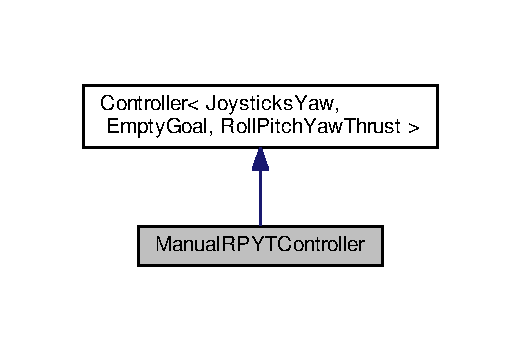
\includegraphics[width=250pt]{classManualRPYTController__inherit__graph}
\end{center}
\end{figure}


Collaboration diagram for Manual\-R\-P\-Y\-T\-Controller\-:\nopagebreak
\begin{figure}[H]
\begin{center}
\leavevmode
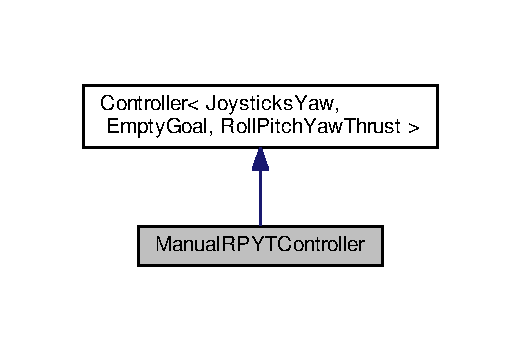
\includegraphics[width=250pt]{classManualRPYTController__coll__graph}
\end{center}
\end{figure}
\subsection*{Public Member Functions}
\begin{DoxyCompactItemize}
\item 
virtual \hyperlink{classManualRPYTController_ac85b5cc721914cb7d265a35b155037af}{$\sim$\-Manual\-R\-P\-Y\-T\-Controller} ()
\begin{DoxyCompactList}\small\item\em Destructor. \end{DoxyCompactList}\end{DoxyCompactItemize}
\subsection*{Protected Member Functions}
\begin{DoxyCompactItemize}
\item 
virtual \hyperlink{structRollPitchYawThrust}{Roll\-Pitch\-Yaw\-Thrust} \hyperlink{classManualRPYTController_ae29c56af6d0bc913d357c7849201c8fb}{run\-Implementation} (\hyperlink{structJoysticksYaw}{Joysticks\-Yaw} sensor\-\_\-data, \hyperlink{structEmptyGoal}{Empty\-Goal} goal)
\begin{DoxyCompactList}\small\item\em Run the control loop. Converts Joystick commands to R\-P\-Y\-T. \end{DoxyCompactList}\end{DoxyCompactItemize}


\subsection{Detailed Description}
A controller that passes joystick commands to a drone's R\-P\-Y\-T controller. 

\subsection{Constructor \& Destructor Documentation}
\hypertarget{classManualRPYTController_ac85b5cc721914cb7d265a35b155037af}{\index{Manual\-R\-P\-Y\-T\-Controller@{Manual\-R\-P\-Y\-T\-Controller}!$\sim$\-Manual\-R\-P\-Y\-T\-Controller@{$\sim$\-Manual\-R\-P\-Y\-T\-Controller}}
\index{$\sim$\-Manual\-R\-P\-Y\-T\-Controller@{$\sim$\-Manual\-R\-P\-Y\-T\-Controller}!ManualRPYTController@{Manual\-R\-P\-Y\-T\-Controller}}
\subsubsection[{$\sim$\-Manual\-R\-P\-Y\-T\-Controller}]{\setlength{\rightskip}{0pt plus 5cm}virtual Manual\-R\-P\-Y\-T\-Controller\-::$\sim$\-Manual\-R\-P\-Y\-T\-Controller (
\begin{DoxyParamCaption}
{}
\end{DoxyParamCaption}
)\hspace{0.3cm}{\ttfamily [inline]}, {\ttfamily [virtual]}}}\label{classManualRPYTController_ac85b5cc721914cb7d265a35b155037af}


Destructor. 



\subsection{Member Function Documentation}
\hypertarget{classManualRPYTController_ae29c56af6d0bc913d357c7849201c8fb}{\index{Manual\-R\-P\-Y\-T\-Controller@{Manual\-R\-P\-Y\-T\-Controller}!run\-Implementation@{run\-Implementation}}
\index{run\-Implementation@{run\-Implementation}!ManualRPYTController@{Manual\-R\-P\-Y\-T\-Controller}}
\subsubsection[{run\-Implementation}]{\setlength{\rightskip}{0pt plus 5cm}{\bf Roll\-Pitch\-Yaw\-Thrust} Manual\-R\-P\-Y\-T\-Controller\-::run\-Implementation (
\begin{DoxyParamCaption}
\item[{{\bf Joysticks\-Yaw}}]{sensor\-\_\-data, }
\item[{{\bf Empty\-Goal}}]{goal}
\end{DoxyParamCaption}
)\hspace{0.3cm}{\ttfamily [protected]}, {\ttfamily [virtual]}}}\label{classManualRPYTController_ae29c56af6d0bc913d357c7849201c8fb}


Run the control loop. Converts Joystick commands to R\-P\-Y\-T. 


\begin{DoxyParams}{Parameters}
{\em sensor\-\_\-data} & Joystick commands to be converted into R\-P\-Y\-T. \\
\hline
{\em goal} & Goal is not used here \\
\hline
\end{DoxyParams}
\begin{DoxyReturn}{Returns}
R\-P\-Y\-T to send to hardware 
\end{DoxyReturn}
\begin{DoxyRefDesc}{Todo}
\item[\hyperlink{todo__todo000003}{Todo}](matt)\-: need to pass R\-C mapping as parameter \end{DoxyRefDesc}


\begin{DoxyRefDesc}{Todo}
\item[\hyperlink{todo__todo000004}{Todo}](matt)\-: need to pass in frequency as a parameter \end{DoxyRefDesc}


Implements \hyperlink{classController_a9a5a0b6fbedeb476f3a7bfad5f16167e}{Controller$<$ Joysticks\-Yaw, Empty\-Goal, Roll\-Pitch\-Yaw\-Thrust $>$}.



The documentation for this class was generated from the following files\-:\begin{DoxyCompactItemize}
\item 
include/aerial\-\_\-autonomy/controllers/\hyperlink{manual__rpyt__controller_8h}{manual\-\_\-rpyt\-\_\-controller.\-h}\item 
src/controllers/\hyperlink{manual__rpyt__controller_8cpp}{manual\-\_\-rpyt\-\_\-controller.\-cpp}\end{DoxyCompactItemize}

\hypertarget{classManualRPYTControllerDroneConnector}{\section{Manual\-R\-P\-Y\-T\-Controller\-Drone\-Connector Class Reference}
\label{classManualRPYTControllerDroneConnector}\index{Manual\-R\-P\-Y\-T\-Controller\-Drone\-Connector@{Manual\-R\-P\-Y\-T\-Controller\-Drone\-Connector}}
}


Maps Joystick goals to rpythrust commands to quadrotor.  




{\ttfamily \#include $<$manual\-\_\-rpyt\-\_\-controller\-\_\-drone\-\_\-connector.\-h$>$}



Inheritance diagram for Manual\-R\-P\-Y\-T\-Controller\-Drone\-Connector\-:\nopagebreak
\begin{figure}[H]
\begin{center}
\leavevmode
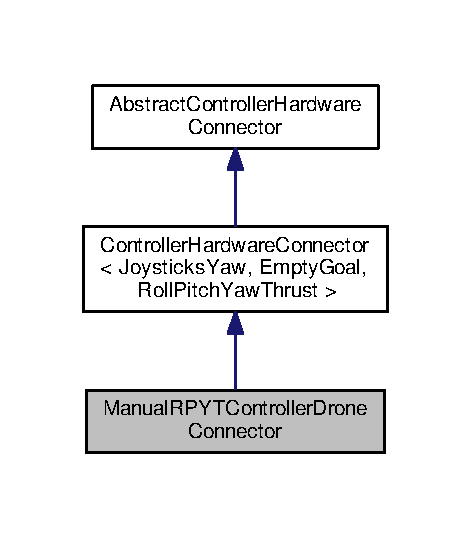
\includegraphics[width=226pt]{classManualRPYTControllerDroneConnector__inherit__graph}
\end{center}
\end{figure}


Collaboration diagram for Manual\-R\-P\-Y\-T\-Controller\-Drone\-Connector\-:\nopagebreak
\begin{figure}[H]
\begin{center}
\leavevmode
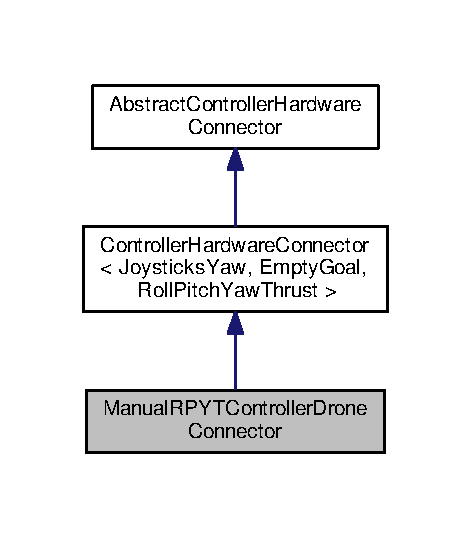
\includegraphics[width=226pt]{classManualRPYTControllerDroneConnector__coll__graph}
\end{center}
\end{figure}
\subsection*{Public Member Functions}
\begin{DoxyCompactItemize}
\item 
\hyperlink{classManualRPYTControllerDroneConnector_a1e9d3f52b19ed5d89b00d6358f826f9b}{Manual\-R\-P\-Y\-T\-Controller\-Drone\-Connector} (parsernode\-::\-Parser \&drone\-\_\-hardware, \hyperlink{classController}{Controller}$<$ \hyperlink{structJoysticksYaw}{Joysticks\-Yaw}, \hyperlink{structEmptyGoal}{Empty\-Goal}, \hyperlink{structRollPitchYawThrust}{Roll\-Pitch\-Yaw\-Thrust} $>$ \&controller)
\begin{DoxyCompactList}\small\item\em Constructor. \end{DoxyCompactList}\end{DoxyCompactItemize}
\subsection*{Protected Member Functions}
\begin{DoxyCompactItemize}
\item 
virtual \hyperlink{structJoysticksYaw}{Joysticks\-Yaw} \hyperlink{classManualRPYTControllerDroneConnector_a6c47447c98dd1528703355f9f60f1d50}{extract\-Sensor\-Data} ()
\begin{DoxyCompactList}\small\item\em Extracts joystick commands and current yaw from hardware. \end{DoxyCompactList}\item 
virtual void \hyperlink{classManualRPYTControllerDroneConnector_a34bde89c4b4f2d0de000b4ccbfc719c4}{send\-Hardware\-Commands} (\hyperlink{structRollPitchYawThrust}{Roll\-Pitch\-Yaw\-Thrust} controls)
\begin{DoxyCompactList}\small\item\em Send R\-P\-Y\-T commands to hardware. \end{DoxyCompactList}\end{DoxyCompactItemize}
\subsection*{Additional Inherited Members}


\subsection{Detailed Description}
Maps Joystick goals to rpythrust commands to quadrotor. 

\subsection{Constructor \& Destructor Documentation}
\hypertarget{classManualRPYTControllerDroneConnector_a1e9d3f52b19ed5d89b00d6358f826f9b}{\index{Manual\-R\-P\-Y\-T\-Controller\-Drone\-Connector@{Manual\-R\-P\-Y\-T\-Controller\-Drone\-Connector}!Manual\-R\-P\-Y\-T\-Controller\-Drone\-Connector@{Manual\-R\-P\-Y\-T\-Controller\-Drone\-Connector}}
\index{Manual\-R\-P\-Y\-T\-Controller\-Drone\-Connector@{Manual\-R\-P\-Y\-T\-Controller\-Drone\-Connector}!ManualRPYTControllerDroneConnector@{Manual\-R\-P\-Y\-T\-Controller\-Drone\-Connector}}
\subsubsection[{Manual\-R\-P\-Y\-T\-Controller\-Drone\-Connector}]{\setlength{\rightskip}{0pt plus 5cm}Manual\-R\-P\-Y\-T\-Controller\-Drone\-Connector\-::\-Manual\-R\-P\-Y\-T\-Controller\-Drone\-Connector (
\begin{DoxyParamCaption}
\item[{parsernode\-::\-Parser \&}]{drone\-\_\-hardware, }
\item[{{\bf Controller}$<$ {\bf Joysticks\-Yaw}, {\bf Empty\-Goal}, {\bf Roll\-Pitch\-Yaw\-Thrust} $>$ \&}]{controller}
\end{DoxyParamCaption}
)\hspace{0.3cm}{\ttfamily [inline]}}}\label{classManualRPYTControllerDroneConnector_a1e9d3f52b19ed5d89b00d6358f826f9b}


Constructor. 

Store drone hardware with hardware type as U\-A\-V. Uses parsernode\-::\-Parser\-::cmdrpythrust function.


\begin{DoxyParams}{Parameters}
{\em drone\-\_\-hardware} & Drone hardware used to send commands \\
\hline
{\em controller} & Rpy\-Thrust controller \\
\hline
\end{DoxyParams}


\subsection{Member Function Documentation}
\hypertarget{classManualRPYTControllerDroneConnector_a6c47447c98dd1528703355f9f60f1d50}{\index{Manual\-R\-P\-Y\-T\-Controller\-Drone\-Connector@{Manual\-R\-P\-Y\-T\-Controller\-Drone\-Connector}!extract\-Sensor\-Data@{extract\-Sensor\-Data}}
\index{extract\-Sensor\-Data@{extract\-Sensor\-Data}!ManualRPYTControllerDroneConnector@{Manual\-R\-P\-Y\-T\-Controller\-Drone\-Connector}}
\subsubsection[{extract\-Sensor\-Data}]{\setlength{\rightskip}{0pt plus 5cm}{\bf Joysticks\-Yaw} Manual\-R\-P\-Y\-T\-Controller\-Drone\-Connector\-::extract\-Sensor\-Data (
\begin{DoxyParamCaption}
{}
\end{DoxyParamCaption}
)\hspace{0.3cm}{\ttfamily [protected]}, {\ttfamily [virtual]}}}\label{classManualRPYTControllerDroneConnector_a6c47447c98dd1528703355f9f60f1d50}


Extracts joystick commands and current yaw from hardware. 

\begin{DoxyReturn}{Returns}
Joystick commands and current yaw 
\end{DoxyReturn}


Implements \hyperlink{classControllerHardwareConnector_af6952c0d8829b93557eb7d8887bebd63}{Controller\-Hardware\-Connector$<$ Joysticks\-Yaw, Empty\-Goal, Roll\-Pitch\-Yaw\-Thrust $>$}.

\hypertarget{classManualRPYTControllerDroneConnector_a34bde89c4b4f2d0de000b4ccbfc719c4}{\index{Manual\-R\-P\-Y\-T\-Controller\-Drone\-Connector@{Manual\-R\-P\-Y\-T\-Controller\-Drone\-Connector}!send\-Hardware\-Commands@{send\-Hardware\-Commands}}
\index{send\-Hardware\-Commands@{send\-Hardware\-Commands}!ManualRPYTControllerDroneConnector@{Manual\-R\-P\-Y\-T\-Controller\-Drone\-Connector}}
\subsubsection[{send\-Hardware\-Commands}]{\setlength{\rightskip}{0pt plus 5cm}void Manual\-R\-P\-Y\-T\-Controller\-Drone\-Connector\-::send\-Hardware\-Commands (
\begin{DoxyParamCaption}
\item[{{\bf Roll\-Pitch\-Yaw\-Thrust}}]{controls}
\end{DoxyParamCaption}
)\hspace{0.3cm}{\ttfamily [protected]}, {\ttfamily [virtual]}}}\label{classManualRPYTControllerDroneConnector_a34bde89c4b4f2d0de000b4ccbfc719c4}


Send R\-P\-Y\-T commands to hardware. 


\begin{DoxyParams}{Parameters}
{\em controls} & R\-P\-Y\-T command to send to drone \\
\hline
\end{DoxyParams}


Implements \hyperlink{classControllerHardwareConnector_a5fc86156d5c747aba36497732962d6d0}{Controller\-Hardware\-Connector$<$ Joysticks\-Yaw, Empty\-Goal, Roll\-Pitch\-Yaw\-Thrust $>$}.



The documentation for this class was generated from the following files\-:\begin{DoxyCompactItemize}
\item 
include/aerial\-\_\-autonomy/controller\-\_\-hardware\-\_\-connectors/\hyperlink{manual__rpyt__controller__drone__connector_8h}{manual\-\_\-rpyt\-\_\-controller\-\_\-drone\-\_\-connector.\-h}\item 
src/controller\-\_\-hardware\-\_\-connectors/\hyperlink{manual__rpyt__controller__drone__connector_8cpp}{manual\-\_\-rpyt\-\_\-controller\-\_\-drone\-\_\-connector.\-cpp}\end{DoxyCompactItemize}

\hypertarget{classOnboardSystemHandler}{\section{Onboard\-System\-Handler$<$ Logic\-State\-Machine\-T, Event\-Manager\-T $>$ Class Template Reference}
\label{classOnboardSystemHandler}\index{Onboard\-System\-Handler$<$ Logic\-State\-Machine\-T, Event\-Manager\-T $>$@{Onboard\-System\-Handler$<$ Logic\-State\-Machine\-T, Event\-Manager\-T $>$}}
}


Owns all of the autonomous system components and is responsible for thread management.  




{\ttfamily \#include $<$onboard\-\_\-system\-\_\-handler.\-h$>$}

\subsection*{Public Member Functions}
\begin{DoxyCompactItemize}
\item 
\hyperlink{classOnboardSystemHandler_a50433d9368004a07ee1d410516f16d0f}{Onboard\-System\-Handler} (ros\-::\-Node\-Handle \&nh, Onboard\-System\-Handler\-Config \&config)
\begin{DoxyCompactList}\small\item\em Constructor. \end{DoxyCompactList}\item 
\hyperlink{classOnboardSystemHandler_a6ab804a5c415b7dcde04babd918738e2}{Onboard\-System\-Handler} (const \hyperlink{classOnboardSystemHandler}{Onboard\-System\-Handler} \&)=delete
\begin{DoxyCompactList}\small\item\em Delete copy constructor. \end{DoxyCompactList}\item 
bool \hyperlink{classOnboardSystemHandler_afd53ef53f99eb8b8af8b15dd1b059eba}{is\-Connected} ()
\begin{DoxyCompactList}\small\item\em Checks if internal R\-O\-S topics are connected. \end{DoxyCompactList}\item 
parsernode\-::common\-::quaddata \hyperlink{classOnboardSystemHandler_ad39e806fb8edd6281d10b8575345ad6d}{get\-U\-A\-V\-Data} ()
\begin{DoxyCompactList}\small\item\em Get U\-A\-V state. \end{DoxyCompactList}\end{DoxyCompactItemize}


\subsection{Detailed Description}
\subsubsection*{template$<$class Logic\-State\-Machine\-T, class Event\-Manager\-T$>$class Onboard\-System\-Handler$<$ Logic\-State\-Machine\-T, Event\-Manager\-T $>$}

Owns all of the autonomous system components and is responsible for thread management. 


\begin{DoxyTemplParams}{Template Parameters}
{\em Logic\-State\-Machine\-T} & Logic state machine to use \\
\hline
{\em Event\-Manager\-T} & Event manager to use \\
\hline
\end{DoxyTemplParams}


\subsection{Constructor \& Destructor Documentation}
\hypertarget{classOnboardSystemHandler_a50433d9368004a07ee1d410516f16d0f}{\index{Onboard\-System\-Handler@{Onboard\-System\-Handler}!Onboard\-System\-Handler@{Onboard\-System\-Handler}}
\index{Onboard\-System\-Handler@{Onboard\-System\-Handler}!OnboardSystemHandler@{Onboard\-System\-Handler}}
\subsubsection[{Onboard\-System\-Handler}]{\setlength{\rightskip}{0pt plus 5cm}template$<$class Logic\-State\-Machine\-T , class Event\-Manager\-T $>$ {\bf Onboard\-System\-Handler}$<$ Logic\-State\-Machine\-T, Event\-Manager\-T $>$\-::{\bf Onboard\-System\-Handler} (
\begin{DoxyParamCaption}
\item[{ros\-::\-Node\-Handle \&}]{nh, }
\item[{Onboard\-System\-Handler\-Config \&}]{config}
\end{DoxyParamCaption}
)\hspace{0.3cm}{\ttfamily [inline]}}}\label{classOnboardSystemHandler_a50433d9368004a07ee1d410516f16d0f}


Constructor. 


\begin{DoxyParams}{Parameters}
{\em nh} & Node\-Handle to use for event and command subscription \\
\hline
{\em config} & Proto configuration parameters \\
\hline
\end{DoxyParams}
\hypertarget{classOnboardSystemHandler_a6ab804a5c415b7dcde04babd918738e2}{\index{Onboard\-System\-Handler@{Onboard\-System\-Handler}!Onboard\-System\-Handler@{Onboard\-System\-Handler}}
\index{Onboard\-System\-Handler@{Onboard\-System\-Handler}!OnboardSystemHandler@{Onboard\-System\-Handler}}
\subsubsection[{Onboard\-System\-Handler}]{\setlength{\rightskip}{0pt plus 5cm}template$<$class Logic\-State\-Machine\-T , class Event\-Manager\-T $>$ {\bf Onboard\-System\-Handler}$<$ Logic\-State\-Machine\-T, Event\-Manager\-T $>$\-::{\bf Onboard\-System\-Handler} (
\begin{DoxyParamCaption}
\item[{const {\bf Onboard\-System\-Handler}$<$ Logic\-State\-Machine\-T, Event\-Manager\-T $>$ \&}]{}
\end{DoxyParamCaption}
)\hspace{0.3cm}{\ttfamily [delete]}}}\label{classOnboardSystemHandler_a6ab804a5c415b7dcde04babd918738e2}


Delete copy constructor. 



\subsection{Member Function Documentation}
\hypertarget{classOnboardSystemHandler_ad39e806fb8edd6281d10b8575345ad6d}{\index{Onboard\-System\-Handler@{Onboard\-System\-Handler}!get\-U\-A\-V\-Data@{get\-U\-A\-V\-Data}}
\index{get\-U\-A\-V\-Data@{get\-U\-A\-V\-Data}!OnboardSystemHandler@{Onboard\-System\-Handler}}
\subsubsection[{get\-U\-A\-V\-Data}]{\setlength{\rightskip}{0pt plus 5cm}template$<$class Logic\-State\-Machine\-T , class Event\-Manager\-T $>$ parsernode\-::common\-::quaddata {\bf Onboard\-System\-Handler}$<$ Logic\-State\-Machine\-T, Event\-Manager\-T $>$\-::get\-U\-A\-V\-Data (
\begin{DoxyParamCaption}
{}
\end{DoxyParamCaption}
)\hspace{0.3cm}{\ttfamily [inline]}}}\label{classOnboardSystemHandler_ad39e806fb8edd6281d10b8575345ad6d}


Get U\-A\-V state. 

\begin{DoxyReturn}{Returns}
The U\-A\-V state 
\end{DoxyReturn}
\hypertarget{classOnboardSystemHandler_afd53ef53f99eb8b8af8b15dd1b059eba}{\index{Onboard\-System\-Handler@{Onboard\-System\-Handler}!is\-Connected@{is\-Connected}}
\index{is\-Connected@{is\-Connected}!OnboardSystemHandler@{Onboard\-System\-Handler}}
\subsubsection[{is\-Connected}]{\setlength{\rightskip}{0pt plus 5cm}template$<$class Logic\-State\-Machine\-T , class Event\-Manager\-T $>$ bool {\bf Onboard\-System\-Handler}$<$ Logic\-State\-Machine\-T, Event\-Manager\-T $>$\-::is\-Connected (
\begin{DoxyParamCaption}
{}
\end{DoxyParamCaption}
)\hspace{0.3cm}{\ttfamily [inline]}}}\label{classOnboardSystemHandler_afd53ef53f99eb8b8af8b15dd1b059eba}


Checks if internal R\-O\-S topics are connected. 

\begin{DoxyReturn}{Returns}
Returns true if connected and false otherwise 
\end{DoxyReturn}


The documentation for this class was generated from the following file\-:\begin{DoxyCompactItemize}
\item 
include/aerial\-\_\-autonomy/\hyperlink{onboard__system__handler_8h}{onboard\-\_\-system\-\_\-handler.\-h}\end{DoxyCompactItemize}

\hypertarget{structPosition}{\section{Position Struct Reference}
\label{structPosition}\index{Position@{Position}}
}


Store 3\-D position.  




{\ttfamily \#include $<$position.\-h$>$}



Inheritance diagram for Position\-:\nopagebreak
\begin{figure}[H]
\begin{center}
\leavevmode
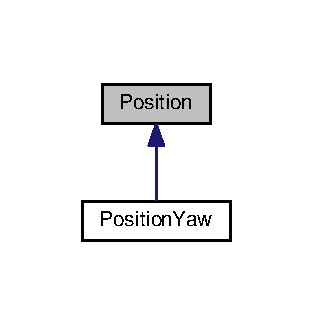
\includegraphics[width=150pt]{structPosition__inherit__graph}
\end{center}
\end{figure}
\subsection*{Public Member Functions}
\begin{DoxyCompactItemize}
\item 
\hyperlink{structPosition_a369a577425f8ba02e8750d04b6a088db}{Position} ()
\begin{DoxyCompactList}\small\item\em Implicit constructor Instantiate position to (0,0,0)m. \end{DoxyCompactList}\item 
\hyperlink{structPosition_a039074b4b66e3b570ea2f4e14583b0e0}{Position} (double \hyperlink{structPosition_a9abbe738bad177de91fe4774099c1260}{x}, double \hyperlink{structPosition_a75f48c2a1d2c7131b8be1a0687ae72c8}{y}, double \hyperlink{structPosition_ab26043bc2f8f6094818c17dd44e43228}{z})
\begin{DoxyCompactList}\small\item\em Explicit constructor. \end{DoxyCompactList}\item 
bool \hyperlink{structPosition_abf82a72c9a5f64a4dfce9691bd3010ed}{operator==} (const \hyperlink{structPosition}{Position} \&p) const 
\begin{DoxyCompactList}\small\item\em Compare two positions. \end{DoxyCompactList}\item 
bool \hyperlink{structPosition_aac2ef88bfed1a5370bb4c2921046e9c0}{operator!=} (const \hyperlink{structPosition}{Position} \&p) const 
\begin{DoxyCompactList}\small\item\em Compare two positions. \end{DoxyCompactList}\end{DoxyCompactItemize}
\subsection*{Public Attributes}
\begin{DoxyCompactItemize}
\item 
double \hyperlink{structPosition_a9abbe738bad177de91fe4774099c1260}{x}
\begin{DoxyCompactList}\small\item\em x component in m \end{DoxyCompactList}\item 
double \hyperlink{structPosition_a75f48c2a1d2c7131b8be1a0687ae72c8}{y}
\begin{DoxyCompactList}\small\item\em y component in m \end{DoxyCompactList}\item 
double \hyperlink{structPosition_ab26043bc2f8f6094818c17dd44e43228}{z}
\begin{DoxyCompactList}\small\item\em z component in m \end{DoxyCompactList}\end{DoxyCompactItemize}


\subsection{Detailed Description}
Store 3\-D position. 

\subsection{Constructor \& Destructor Documentation}
\hypertarget{structPosition_a369a577425f8ba02e8750d04b6a088db}{\index{Position@{Position}!Position@{Position}}
\index{Position@{Position}!Position@{Position}}
\subsubsection[{Position}]{\setlength{\rightskip}{0pt plus 5cm}Position\-::\-Position (
\begin{DoxyParamCaption}
{}
\end{DoxyParamCaption}
)\hspace{0.3cm}{\ttfamily [inline]}}}\label{structPosition_a369a577425f8ba02e8750d04b6a088db}


Implicit constructor Instantiate position to (0,0,0)m. 

\hypertarget{structPosition_a039074b4b66e3b570ea2f4e14583b0e0}{\index{Position@{Position}!Position@{Position}}
\index{Position@{Position}!Position@{Position}}
\subsubsection[{Position}]{\setlength{\rightskip}{0pt plus 5cm}Position\-::\-Position (
\begin{DoxyParamCaption}
\item[{double}]{x, }
\item[{double}]{y, }
\item[{double}]{z}
\end{DoxyParamCaption}
)\hspace{0.3cm}{\ttfamily [inline]}}}\label{structPosition_a039074b4b66e3b570ea2f4e14583b0e0}


Explicit constructor. 


\begin{DoxyParams}{Parameters}
{\em x} & x component in m \\
\hline
{\em y} & y component in m \\
\hline
{\em z} & z component in m \\
\hline
\end{DoxyParams}


\subsection{Member Function Documentation}
\hypertarget{structPosition_aac2ef88bfed1a5370bb4c2921046e9c0}{\index{Position@{Position}!operator!=@{operator!=}}
\index{operator!=@{operator!=}!Position@{Position}}
\subsubsection[{operator!=}]{\setlength{\rightskip}{0pt plus 5cm}bool Position\-::operator!= (
\begin{DoxyParamCaption}
\item[{const {\bf Position} \&}]{p}
\end{DoxyParamCaption}
) const\hspace{0.3cm}{\ttfamily [inline]}}}\label{structPosition_aac2ef88bfed1a5370bb4c2921046e9c0}


Compare two positions. 


\begin{DoxyParams}{Parameters}
{\em p} & \hyperlink{structPosition}{Position} to compare against\\
\hline
\end{DoxyParams}
\begin{DoxyReturn}{Returns}
True if two positions are not same 
\end{DoxyReturn}
\hypertarget{structPosition_abf82a72c9a5f64a4dfce9691bd3010ed}{\index{Position@{Position}!operator==@{operator==}}
\index{operator==@{operator==}!Position@{Position}}
\subsubsection[{operator==}]{\setlength{\rightskip}{0pt plus 5cm}bool Position\-::operator== (
\begin{DoxyParamCaption}
\item[{const {\bf Position} \&}]{p}
\end{DoxyParamCaption}
) const\hspace{0.3cm}{\ttfamily [inline]}}}\label{structPosition_abf82a72c9a5f64a4dfce9691bd3010ed}


Compare two positions. 


\begin{DoxyParams}{Parameters}
{\em p} & \hyperlink{structPosition}{Position} to compare against\\
\hline
\end{DoxyParams}
\begin{DoxyReturn}{Returns}
True if two positions are same 
\end{DoxyReturn}


\subsection{Member Data Documentation}
\hypertarget{structPosition_a9abbe738bad177de91fe4774099c1260}{\index{Position@{Position}!x@{x}}
\index{x@{x}!Position@{Position}}
\subsubsection[{x}]{\setlength{\rightskip}{0pt plus 5cm}double Position\-::x}}\label{structPosition_a9abbe738bad177de91fe4774099c1260}


x component in m 

\hypertarget{structPosition_a75f48c2a1d2c7131b8be1a0687ae72c8}{\index{Position@{Position}!y@{y}}
\index{y@{y}!Position@{Position}}
\subsubsection[{y}]{\setlength{\rightskip}{0pt plus 5cm}double Position\-::y}}\label{structPosition_a75f48c2a1d2c7131b8be1a0687ae72c8}


y component in m 

\hypertarget{structPosition_ab26043bc2f8f6094818c17dd44e43228}{\index{Position@{Position}!z@{z}}
\index{z@{z}!Position@{Position}}
\subsubsection[{z}]{\setlength{\rightskip}{0pt plus 5cm}double Position\-::z}}\label{structPosition_ab26043bc2f8f6094818c17dd44e43228}


z component in m 



The documentation for this struct was generated from the following file\-:\begin{DoxyCompactItemize}
\item 
include/aerial\-\_\-autonomy/types/\hyperlink{position_8h}{position.\-h}\end{DoxyCompactItemize}

\hypertarget{structPositionControlAbortActionFunctor__}{\section{Position\-Control\-Abort\-Action\-Functor\-\_\-$<$ Logic\-State\-Machine\-T $>$ Struct Template Reference}
\label{structPositionControlAbortActionFunctor__}\index{Position\-Control\-Abort\-Action\-Functor\-\_\-$<$ Logic\-State\-Machine\-T $>$@{Position\-Control\-Abort\-Action\-Functor\-\_\-$<$ Logic\-State\-Machine\-T $>$}}
}


Transition action to perform when aborting position control.  




{\ttfamily \#include $<$position\-\_\-control\-\_\-functors.\-h$>$}



Inheritance diagram for Position\-Control\-Abort\-Action\-Functor\-\_\-$<$ Logic\-State\-Machine\-T $>$\-:\nopagebreak
\begin{figure}[H]
\begin{center}
\leavevmode
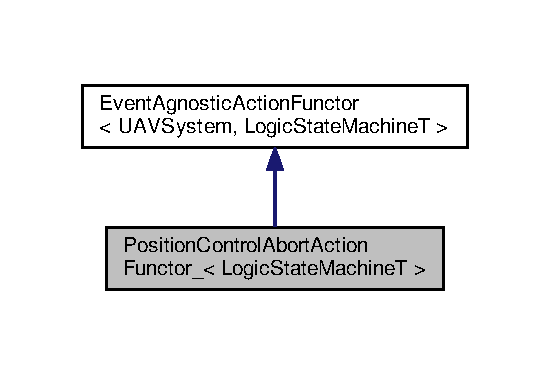
\includegraphics[width=264pt]{structPositionControlAbortActionFunctor____inherit__graph}
\end{center}
\end{figure}


Collaboration diagram for Position\-Control\-Abort\-Action\-Functor\-\_\-$<$ Logic\-State\-Machine\-T $>$\-:\nopagebreak
\begin{figure}[H]
\begin{center}
\leavevmode
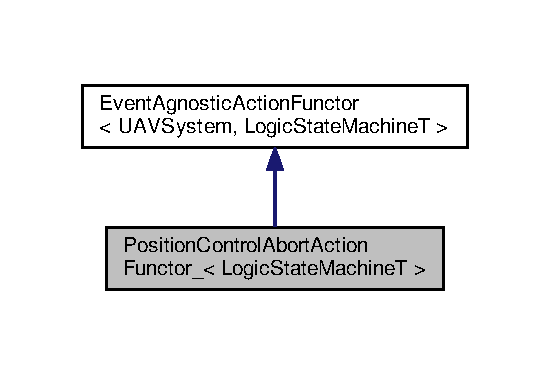
\includegraphics[width=264pt]{structPositionControlAbortActionFunctor____coll__graph}
\end{center}
\end{figure}
\subsection*{Public Member Functions}
\begin{DoxyCompactItemize}
\item 
void \hyperlink{structPositionControlAbortActionFunctor___a04152d311e51abb5b330ee74b3c29702}{run} (\hyperlink{classUAVSystem}{U\-A\-V\-System} \&robot\-\_\-system, Logic\-State\-Machine\-T \&)
\begin{DoxyCompactList}\small\item\em Override this run function for different sub classes. This function performs the logic checking for each state. \end{DoxyCompactList}\end{DoxyCompactItemize}


\subsection{Detailed Description}
\subsubsection*{template$<$class Logic\-State\-Machine\-T$>$struct Position\-Control\-Abort\-Action\-Functor\-\_\-$<$ Logic\-State\-Machine\-T $>$}

Transition action to perform when aborting position control. 


\begin{DoxyTemplParams}{Template Parameters}
{\em Logic\-State\-Machine\-T} & Logic state machine used to process events \\
\hline
\end{DoxyTemplParams}


\subsection{Member Function Documentation}
\hypertarget{structPositionControlAbortActionFunctor___a04152d311e51abb5b330ee74b3c29702}{\index{Position\-Control\-Abort\-Action\-Functor\-\_\-@{Position\-Control\-Abort\-Action\-Functor\-\_\-}!run@{run}}
\index{run@{run}!PositionControlAbortActionFunctor_@{Position\-Control\-Abort\-Action\-Functor\-\_\-}}
\subsubsection[{run}]{\setlength{\rightskip}{0pt plus 5cm}template$<$class Logic\-State\-Machine\-T $>$ void {\bf Position\-Control\-Abort\-Action\-Functor\-\_\-}$<$ Logic\-State\-Machine\-T $>$\-::run (
\begin{DoxyParamCaption}
\item[{{\bf U\-A\-V\-System} \&}]{robot\-\_\-system, }
\item[{Logic\-State\-Machine\-T \&}]{logic\-\_\-state\-\_\-machine}
\end{DoxyParamCaption}
)\hspace{0.3cm}{\ttfamily [inline]}, {\ttfamily [virtual]}}}\label{structPositionControlAbortActionFunctor___a04152d311e51abb5b330ee74b3c29702}


Override this run function for different sub classes. This function performs the logic checking for each state. 


\begin{DoxyParams}{Parameters}
{\em robot\-\_\-system} & Provides sensor data and allows for controlling hardware \\
\hline
{\em logic\-\_\-state\-\_\-machine} & Backend of logic State Machine. can send events using this. \\
\hline
\end{DoxyParams}


Implements \hyperlink{structEventAgnosticActionFunctor_a53a48938d68370ff2ef262222565ffcf}{Event\-Agnostic\-Action\-Functor$<$ U\-A\-V\-System, Logic\-State\-Machine\-T $>$}.



The documentation for this struct was generated from the following file\-:\begin{DoxyCompactItemize}
\item 
include/aerial\-\_\-autonomy/actions\-\_\-guards/\hyperlink{position__control__functors_8h}{position\-\_\-control\-\_\-functors.\-h}\end{DoxyCompactItemize}

\hypertarget{structPositionControlInternalActionFunctor__}{\section{Position\-Control\-Internal\-Action\-Functor\-\_\-$<$ Logic\-State\-Machine\-T $>$ Struct Template Reference}
\label{structPositionControlInternalActionFunctor__}\index{Position\-Control\-Internal\-Action\-Functor\-\_\-$<$ Logic\-State\-Machine\-T $>$@{Position\-Control\-Internal\-Action\-Functor\-\_\-$<$ Logic\-State\-Machine\-T $>$}}
}


Logic to check while reaching a position control goal.  




{\ttfamily \#include $<$position\-\_\-control\-\_\-functors.\-h$>$}



Inheritance diagram for Position\-Control\-Internal\-Action\-Functor\-\_\-$<$ Logic\-State\-Machine\-T $>$\-:\nopagebreak
\begin{figure}[H]
\begin{center}
\leavevmode
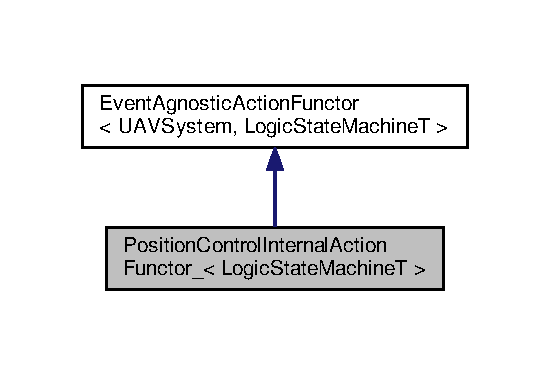
\includegraphics[width=264pt]{structPositionControlInternalActionFunctor____inherit__graph}
\end{center}
\end{figure}


Collaboration diagram for Position\-Control\-Internal\-Action\-Functor\-\_\-$<$ Logic\-State\-Machine\-T $>$\-:\nopagebreak
\begin{figure}[H]
\begin{center}
\leavevmode
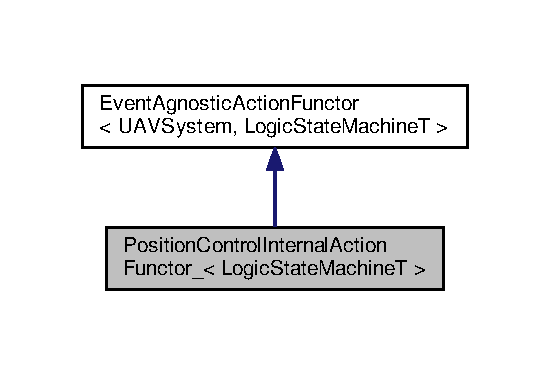
\includegraphics[width=264pt]{structPositionControlInternalActionFunctor____coll__graph}
\end{center}
\end{figure}
\subsection*{Public Member Functions}
\begin{DoxyCompactItemize}
\item 
virtual void \hyperlink{structPositionControlInternalActionFunctor___a81589e5ecfba853969942b9842ac1563}{run} (\hyperlink{classUAVSystem}{U\-A\-V\-System} \&robot\-\_\-system, Logic\-State\-Machine\-T \&logic\-\_\-state\-\_\-machine)
\begin{DoxyCompactList}\small\item\em check if we reached goal and trigger hovering if we reached goal. \end{DoxyCompactList}\end{DoxyCompactItemize}


\subsection{Detailed Description}
\subsubsection*{template$<$class Logic\-State\-Machine\-T$>$struct Position\-Control\-Internal\-Action\-Functor\-\_\-$<$ Logic\-State\-Machine\-T $>$}

Logic to check while reaching a position control goal. 


\begin{DoxyTemplParams}{Template Parameters}
{\em Logic\-State\-Machine\-T} & Logic state machine used to process events \\
\hline
\end{DoxyTemplParams}


\subsection{Member Function Documentation}
\hypertarget{structPositionControlInternalActionFunctor___a81589e5ecfba853969942b9842ac1563}{\index{Position\-Control\-Internal\-Action\-Functor\-\_\-@{Position\-Control\-Internal\-Action\-Functor\-\_\-}!run@{run}}
\index{run@{run}!PositionControlInternalActionFunctor_@{Position\-Control\-Internal\-Action\-Functor\-\_\-}}
\subsubsection[{run}]{\setlength{\rightskip}{0pt plus 5cm}template$<$class Logic\-State\-Machine\-T $>$ virtual void {\bf Position\-Control\-Internal\-Action\-Functor\-\_\-}$<$ Logic\-State\-Machine\-T $>$\-::run (
\begin{DoxyParamCaption}
\item[{{\bf U\-A\-V\-System} \&}]{robot\-\_\-system, }
\item[{Logic\-State\-Machine\-T \&}]{logic\-\_\-state\-\_\-machine}
\end{DoxyParamCaption}
)\hspace{0.3cm}{\ttfamily [inline]}, {\ttfamily [virtual]}}}\label{structPositionControlInternalActionFunctor___a81589e5ecfba853969942b9842ac1563}


check if we reached goal and trigger hovering if we reached goal. 


\begin{DoxyParams}{Parameters}
{\em robot\-\_\-system} & robot system to get sensor data \\
\hline
{\em logic\-\_\-state\-\_\-machine} & logic state machine to trigger events \\
\hline
\end{DoxyParams}


Implements \hyperlink{structEventAgnosticActionFunctor_a53a48938d68370ff2ef262222565ffcf}{Event\-Agnostic\-Action\-Functor$<$ U\-A\-V\-System, Logic\-State\-Machine\-T $>$}.



The documentation for this struct was generated from the following file\-:\begin{DoxyCompactItemize}
\item 
include/aerial\-\_\-autonomy/actions\-\_\-guards/\hyperlink{position__control__functors_8h}{position\-\_\-control\-\_\-functors.\-h}\end{DoxyCompactItemize}

\hypertarget{classPositionControllerDroneConnector}{\section{Position\-Controller\-Drone\-Connector Class Reference}
\label{classPositionControllerDroneConnector}\index{Position\-Controller\-Drone\-Connector@{Position\-Controller\-Drone\-Connector}}
}


Manages communication between a drone plugin and a position controller that outputs position commands.  




{\ttfamily \#include $<$position\-\_\-controller\-\_\-drone\-\_\-connector.\-h$>$}



Inheritance diagram for Position\-Controller\-Drone\-Connector\-:\nopagebreak
\begin{figure}[H]
\begin{center}
\leavevmode
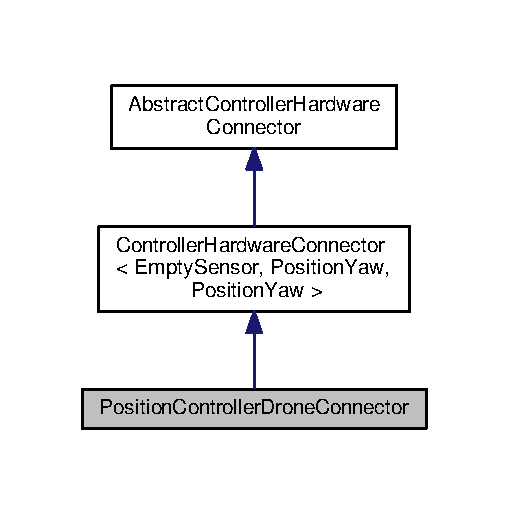
\includegraphics[width=244pt]{classPositionControllerDroneConnector__inherit__graph}
\end{center}
\end{figure}


Collaboration diagram for Position\-Controller\-Drone\-Connector\-:\nopagebreak
\begin{figure}[H]
\begin{center}
\leavevmode
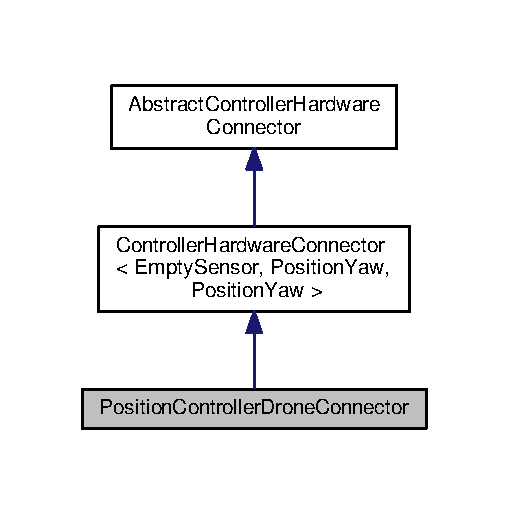
\includegraphics[width=244pt]{classPositionControllerDroneConnector__coll__graph}
\end{center}
\end{figure}
\subsection*{Public Member Functions}
\begin{DoxyCompactItemize}
\item 
\hyperlink{classPositionControllerDroneConnector_a12664821f9f9316f6343b16f3dc9f84f}{Position\-Controller\-Drone\-Connector} (parsernode\-::\-Parser \&drone\-\_\-hardware, \hyperlink{classController}{Controller}$<$ \hyperlink{structEmptySensor}{Empty\-Sensor}, \hyperlink{structPositionYaw}{Position\-Yaw}, \hyperlink{structPositionYaw}{Position\-Yaw} $>$ \&controller)
\begin{DoxyCompactList}\small\item\em Constructor. \end{DoxyCompactList}\end{DoxyCompactItemize}
\subsection*{Protected Member Functions}
\begin{DoxyCompactItemize}
\item 
virtual \hyperlink{structEmptySensor}{Empty\-Sensor} \hyperlink{classPositionControllerDroneConnector_a21859ad4bcc85a907e2e23456869b3d6}{extract\-Sensor\-Data} ()
\begin{DoxyCompactList}\small\item\em does not extract any data since nothing is needed \end{DoxyCompactList}\item 
virtual void \hyperlink{classPositionControllerDroneConnector_a826092eadfbbf9442fa1869fea98070d}{send\-Hardware\-Commands} (\hyperlink{structPositionYaw}{Position\-Yaw} controls)
\begin{DoxyCompactList}\small\item\em Send position commands to hardware. \end{DoxyCompactList}\end{DoxyCompactItemize}
\subsection*{Additional Inherited Members}


\subsection{Detailed Description}
Manages communication between a drone plugin and a position controller that outputs position commands. 

\subsection{Constructor \& Destructor Documentation}
\hypertarget{classPositionControllerDroneConnector_a12664821f9f9316f6343b16f3dc9f84f}{\index{Position\-Controller\-Drone\-Connector@{Position\-Controller\-Drone\-Connector}!Position\-Controller\-Drone\-Connector@{Position\-Controller\-Drone\-Connector}}
\index{Position\-Controller\-Drone\-Connector@{Position\-Controller\-Drone\-Connector}!PositionControllerDroneConnector@{Position\-Controller\-Drone\-Connector}}
\subsubsection[{Position\-Controller\-Drone\-Connector}]{\setlength{\rightskip}{0pt plus 5cm}Position\-Controller\-Drone\-Connector\-::\-Position\-Controller\-Drone\-Connector (
\begin{DoxyParamCaption}
\item[{parsernode\-::\-Parser \&}]{drone\-\_\-hardware, }
\item[{{\bf Controller}$<$ {\bf Empty\-Sensor}, {\bf Position\-Yaw}, {\bf Position\-Yaw} $>$ \&}]{controller}
\end{DoxyParamCaption}
)\hspace{0.3cm}{\ttfamily [inline]}}}\label{classPositionControllerDroneConnector_a12664821f9f9316f6343b16f3dc9f84f}


Constructor. 

Store drone hardware with hardware type as U\-A\-V. Uses parsernode\-::\-Parser\-::cmdwaypoint function.


\begin{DoxyParams}{Parameters}
{\em drone\-\_\-hardware} & Drone hardware used to send commands \\
\hline
{\em controller} & \hyperlink{structPosition}{Position} controller that achieves a desired position, yaw \\
\hline
\end{DoxyParams}


\subsection{Member Function Documentation}
\hypertarget{classPositionControllerDroneConnector_a21859ad4bcc85a907e2e23456869b3d6}{\index{Position\-Controller\-Drone\-Connector@{Position\-Controller\-Drone\-Connector}!extract\-Sensor\-Data@{extract\-Sensor\-Data}}
\index{extract\-Sensor\-Data@{extract\-Sensor\-Data}!PositionControllerDroneConnector@{Position\-Controller\-Drone\-Connector}}
\subsubsection[{extract\-Sensor\-Data}]{\setlength{\rightskip}{0pt plus 5cm}{\bf Empty\-Sensor} Position\-Controller\-Drone\-Connector\-::extract\-Sensor\-Data (
\begin{DoxyParamCaption}
{}
\end{DoxyParamCaption}
)\hspace{0.3cm}{\ttfamily [protected]}, {\ttfamily [virtual]}}}\label{classPositionControllerDroneConnector_a21859ad4bcc85a907e2e23456869b3d6}


does not extract any data since nothing is needed 

\begin{DoxyReturn}{Returns}
empty data structure 
\end{DoxyReturn}


Implements \hyperlink{classControllerHardwareConnector_af6952c0d8829b93557eb7d8887bebd63}{Controller\-Hardware\-Connector$<$ Empty\-Sensor, Position\-Yaw, Position\-Yaw $>$}.

\hypertarget{classPositionControllerDroneConnector_a826092eadfbbf9442fa1869fea98070d}{\index{Position\-Controller\-Drone\-Connector@{Position\-Controller\-Drone\-Connector}!send\-Hardware\-Commands@{send\-Hardware\-Commands}}
\index{send\-Hardware\-Commands@{send\-Hardware\-Commands}!PositionControllerDroneConnector@{Position\-Controller\-Drone\-Connector}}
\subsubsection[{send\-Hardware\-Commands}]{\setlength{\rightskip}{0pt plus 5cm}void Position\-Controller\-Drone\-Connector\-::send\-Hardware\-Commands (
\begin{DoxyParamCaption}
\item[{{\bf Position\-Yaw}}]{controls}
\end{DoxyParamCaption}
)\hspace{0.3cm}{\ttfamily [protected]}, {\ttfamily [virtual]}}}\label{classPositionControllerDroneConnector_a826092eadfbbf9442fa1869fea98070d}


Send position commands to hardware. 


\begin{DoxyParams}{Parameters}
{\em controls} & position command to send to U\-A\-V \\
\hline
\end{DoxyParams}


Implements \hyperlink{classControllerHardwareConnector_a5fc86156d5c747aba36497732962d6d0}{Controller\-Hardware\-Connector$<$ Empty\-Sensor, Position\-Yaw, Position\-Yaw $>$}.



The documentation for this class was generated from the following files\-:\begin{DoxyCompactItemize}
\item 
include/aerial\-\_\-autonomy/controller\-\_\-hardware\-\_\-connectors/\hyperlink{position__controller__drone__connector_8h}{position\-\_\-controller\-\_\-drone\-\_\-connector.\-h}\item 
src/controller\-\_\-hardware\-\_\-connectors/\hyperlink{position__controller__drone__connector_8cpp}{position\-\_\-controller\-\_\-drone\-\_\-connector.\-cpp}\end{DoxyCompactItemize}

\hypertarget{structPositionControlTransitionActionFunctor__}{\section{Position\-Control\-Transition\-Action\-Functor\-\_\-$<$ Logic\-State\-Machine\-T $>$ Struct Template Reference}
\label{structPositionControlTransitionActionFunctor__}\index{Position\-Control\-Transition\-Action\-Functor\-\_\-$<$ Logic\-State\-Machine\-T $>$@{Position\-Control\-Transition\-Action\-Functor\-\_\-$<$ Logic\-State\-Machine\-T $>$}}
}


Transition action to perform when going into position control mode.  




{\ttfamily \#include $<$position\-\_\-control\-\_\-functors.\-h$>$}



Inheritance diagram for Position\-Control\-Transition\-Action\-Functor\-\_\-$<$ Logic\-State\-Machine\-T $>$\-:\nopagebreak
\begin{figure}[H]
\begin{center}
\leavevmode
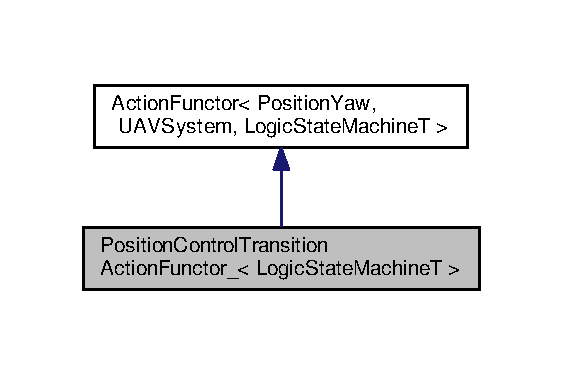
\includegraphics[width=270pt]{structPositionControlTransitionActionFunctor____inherit__graph}
\end{center}
\end{figure}


Collaboration diagram for Position\-Control\-Transition\-Action\-Functor\-\_\-$<$ Logic\-State\-Machine\-T $>$\-:\nopagebreak
\begin{figure}[H]
\begin{center}
\leavevmode
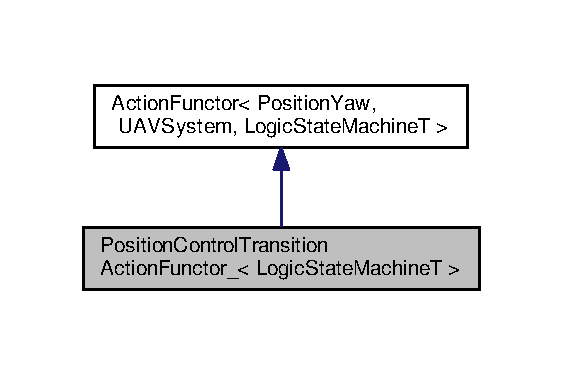
\includegraphics[width=270pt]{structPositionControlTransitionActionFunctor____coll__graph}
\end{center}
\end{figure}
\subsection*{Public Member Functions}
\begin{DoxyCompactItemize}
\item 
void \hyperlink{structPositionControlTransitionActionFunctor___a4970bb461809ffa30984e16902bb8aaa}{run} (const \hyperlink{structPositionYaw}{Position\-Yaw} \&goal, \hyperlink{classUAVSystem}{U\-A\-V\-System} \&robot\-\_\-system, Logic\-State\-Machine\-T \&)
\begin{DoxyCompactList}\small\item\em Override this run function for different sub classes. This function performs the logic checking for each state. \end{DoxyCompactList}\end{DoxyCompactItemize}


\subsection{Detailed Description}
\subsubsection*{template$<$class Logic\-State\-Machine\-T$>$struct Position\-Control\-Transition\-Action\-Functor\-\_\-$<$ Logic\-State\-Machine\-T $>$}

Transition action to perform when going into position control mode. 


\begin{DoxyTemplParams}{Template Parameters}
{\em Logic\-State\-Machine\-T} & Logic state machine used to process events \\
\hline
\end{DoxyTemplParams}


\subsection{Member Function Documentation}
\hypertarget{structPositionControlTransitionActionFunctor___a4970bb461809ffa30984e16902bb8aaa}{\index{Position\-Control\-Transition\-Action\-Functor\-\_\-@{Position\-Control\-Transition\-Action\-Functor\-\_\-}!run@{run}}
\index{run@{run}!PositionControlTransitionActionFunctor_@{Position\-Control\-Transition\-Action\-Functor\-\_\-}}
\subsubsection[{run}]{\setlength{\rightskip}{0pt plus 5cm}template$<$class Logic\-State\-Machine\-T $>$ void {\bf Position\-Control\-Transition\-Action\-Functor\-\_\-}$<$ Logic\-State\-Machine\-T $>$\-::run (
\begin{DoxyParamCaption}
\item[{const {\bf Position\-Yaw} \&}]{event, }
\item[{{\bf U\-A\-V\-System} \&}]{robot\-\_\-system, }
\item[{Logic\-State\-Machine\-T \&}]{logic\-\_\-state\-\_\-machine}
\end{DoxyParamCaption}
)\hspace{0.3cm}{\ttfamily [inline]}, {\ttfamily [virtual]}}}\label{structPositionControlTransitionActionFunctor___a4970bb461809ffa30984e16902bb8aaa}


Override this run function for different sub classes. This function performs the logic checking for each state. 


\begin{DoxyParams}{Parameters}
{\em robot\-\_\-system} & Provides sensor data and allows for controlling hardware \\
\hline
{\em logic\-\_\-state\-\_\-machine} & Backend of logic State Machine. can send events using this. \\
\hline
{\em event} & Event triggering the action \\
\hline
\end{DoxyParams}


Implements \hyperlink{structActionFunctor_a97250a2cc027dc3ca7d10a975d11a5c7}{Action\-Functor$<$ Position\-Yaw, U\-A\-V\-System, Logic\-State\-Machine\-T $>$}.



The documentation for this struct was generated from the following file\-:\begin{DoxyCompactItemize}
\item 
include/aerial\-\_\-autonomy/actions\-\_\-guards/\hyperlink{position__control__functors_8h}{position\-\_\-control\-\_\-functors.\-h}\end{DoxyCompactItemize}

\hypertarget{structPositionControlTransitionGuardFunctor__}{\section{Position\-Control\-Transition\-Guard\-Functor\-\_\-$<$ Logic\-State\-Machine\-T $>$ Struct Template Reference}
\label{structPositionControlTransitionGuardFunctor__}\index{Position\-Control\-Transition\-Guard\-Functor\-\_\-$<$ Logic\-State\-Machine\-T $>$@{Position\-Control\-Transition\-Guard\-Functor\-\_\-$<$ Logic\-State\-Machine\-T $>$}}
}


Guard function to check the goal is within tolerance before starting towards goal.  




{\ttfamily \#include $<$position\-\_\-control\-\_\-functors.\-h$>$}



Inheritance diagram for Position\-Control\-Transition\-Guard\-Functor\-\_\-$<$ Logic\-State\-Machine\-T $>$\-:\nopagebreak
\begin{figure}[H]
\begin{center}
\leavevmode
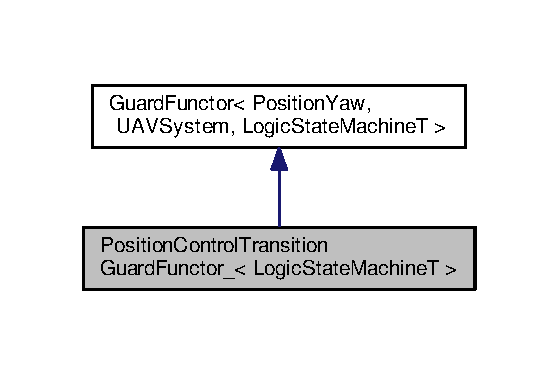
\includegraphics[width=268pt]{structPositionControlTransitionGuardFunctor____inherit__graph}
\end{center}
\end{figure}


Collaboration diagram for Position\-Control\-Transition\-Guard\-Functor\-\_\-$<$ Logic\-State\-Machine\-T $>$\-:\nopagebreak
\begin{figure}[H]
\begin{center}
\leavevmode
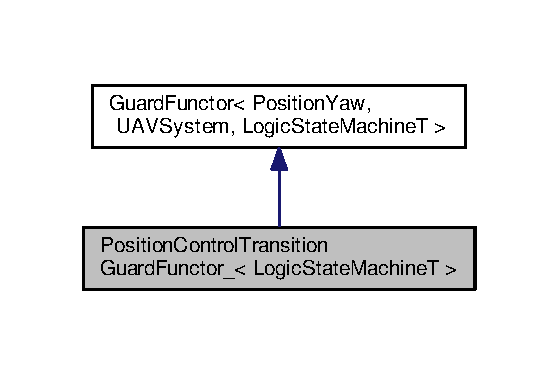
\includegraphics[width=268pt]{structPositionControlTransitionGuardFunctor____coll__graph}
\end{center}
\end{figure}
\subsection*{Public Member Functions}
\begin{DoxyCompactItemize}
\item 
bool \hyperlink{structPositionControlTransitionGuardFunctor___ad0334337a349f9964d0ba781e995dad6}{guard} (const \hyperlink{structPositionYaw}{Position\-Yaw} \&goal, \hyperlink{classUAVSystem}{U\-A\-V\-System} \&robot\-\_\-system, Logic\-State\-Machine\-T \&)
\begin{DoxyCompactList}\small\item\em Override this guard function for different sub classes. This function decides whether to call the run function for each state. \end{DoxyCompactList}\end{DoxyCompactItemize}


\subsection{Detailed Description}
\subsubsection*{template$<$class Logic\-State\-Machine\-T$>$struct Position\-Control\-Transition\-Guard\-Functor\-\_\-$<$ Logic\-State\-Machine\-T $>$}

Guard function to check the goal is within tolerance before starting towards goal. 

\begin{DoxyRefDesc}{Todo}
\item[\hyperlink{todo__todo000009}{Todo}]Use a parameter for setting position tolerance\end{DoxyRefDesc}



\begin{DoxyTemplParams}{Template Parameters}
{\em Logic\-State\-Machine\-T} & Logic state machine used to process events \\
\hline
\end{DoxyTemplParams}


\subsection{Member Function Documentation}
\hypertarget{structPositionControlTransitionGuardFunctor___ad0334337a349f9964d0ba781e995dad6}{\index{Position\-Control\-Transition\-Guard\-Functor\-\_\-@{Position\-Control\-Transition\-Guard\-Functor\-\_\-}!guard@{guard}}
\index{guard@{guard}!PositionControlTransitionGuardFunctor_@{Position\-Control\-Transition\-Guard\-Functor\-\_\-}}
\subsubsection[{guard}]{\setlength{\rightskip}{0pt plus 5cm}template$<$class Logic\-State\-Machine\-T $>$ bool {\bf Position\-Control\-Transition\-Guard\-Functor\-\_\-}$<$ Logic\-State\-Machine\-T $>$\-::guard (
\begin{DoxyParamCaption}
\item[{const {\bf Position\-Yaw} \&}]{event, }
\item[{{\bf U\-A\-V\-System} \&}]{robot\-\_\-system, }
\item[{Logic\-State\-Machine\-T \&}]{logic\-\_\-state\-\_\-machine}
\end{DoxyParamCaption}
)\hspace{0.3cm}{\ttfamily [inline]}, {\ttfamily [virtual]}}}\label{structPositionControlTransitionGuardFunctor___ad0334337a349f9964d0ba781e995dad6}


Override this guard function for different sub classes. This function decides whether to call the run function for each state. 


\begin{DoxyParams}{Parameters}
{\em robot\-\_\-system} & Provides sensor data and allows for controlling hardware \\
\hline
{\em logic\-\_\-state\-\_\-machine} & Backend of logic State Machine. can send events using this. \\
\hline
{\em event} & Event triggering the action \\
\hline
\end{DoxyParams}


Implements \hyperlink{structGuardFunctor_a9f023aa88503d6127cc8280d7dc733b8}{Guard\-Functor$<$ Position\-Yaw, U\-A\-V\-System, Logic\-State\-Machine\-T $>$}.



The documentation for this struct was generated from the following file\-:\begin{DoxyCompactItemize}
\item 
include/aerial\-\_\-autonomy/actions\-\_\-guards/\hyperlink{position__control__functors_8h}{position\-\_\-control\-\_\-functors.\-h}\end{DoxyCompactItemize}

\hypertarget{structPositionYaw}{\section{Position\-Yaw Struct Reference}
\label{structPositionYaw}\index{Position\-Yaw@{Position\-Yaw}}
}


Stores \hyperlink{structPosition}{Position}, yaw. \hyperlink{structPositionYaw}{Position\-Yaw} is used as the goal for U\-A\-V systems.  




{\ttfamily \#include $<$position\-\_\-yaw.\-h$>$}



Inheritance diagram for Position\-Yaw\-:\nopagebreak
\begin{figure}[H]
\begin{center}
\leavevmode
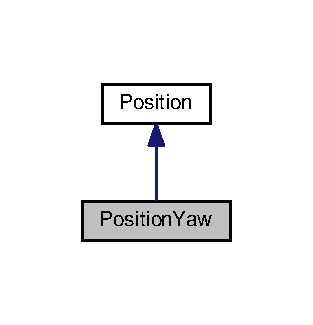
\includegraphics[width=150pt]{structPositionYaw__inherit__graph}
\end{center}
\end{figure}


Collaboration diagram for Position\-Yaw\-:\nopagebreak
\begin{figure}[H]
\begin{center}
\leavevmode
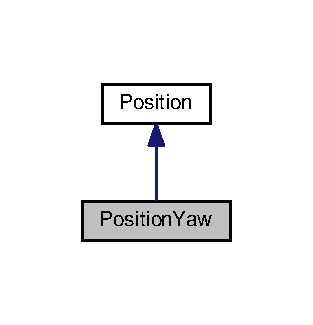
\includegraphics[width=150pt]{structPositionYaw__coll__graph}
\end{center}
\end{figure}
\subsection*{Public Member Functions}
\begin{DoxyCompactItemize}
\item 
\hyperlink{structPositionYaw_a27f89c7703b62e5120c669822c98bcf1}{Position\-Yaw} ()
\begin{DoxyCompactList}\small\item\em Implicit constructor. \end{DoxyCompactList}\item 
\hyperlink{structPositionYaw_a0a03ecfbad91c4c48a6aed44f4933a74}{Position\-Yaw} (\hyperlink{structPosition}{Position} p, double \hyperlink{structPositionYaw_a712a15ba9739cb5f4e31ea973074b8bf}{yaw})
\begin{DoxyCompactList}\small\item\em Explicit constructor that takes in position, yaw. \end{DoxyCompactList}\item 
\hyperlink{structPositionYaw_ae5642ce9e93710cf9cda7263511300f0}{Position\-Yaw} (double \hyperlink{structPosition_a9abbe738bad177de91fe4774099c1260}{x}, double \hyperlink{structPosition_a75f48c2a1d2c7131b8be1a0687ae72c8}{y}, double \hyperlink{structPosition_ab26043bc2f8f6094818c17dd44e43228}{z}, double \hyperlink{structPositionYaw_a712a15ba9739cb5f4e31ea973074b8bf}{yaw})
\begin{DoxyCompactList}\small\item\em Explicit constructor with x,y,z, and yaw. \end{DoxyCompactList}\item 
bool \hyperlink{structPositionYaw_a74eb4415b12fe9c42e102e82d2bd52cb}{operator==} (const \hyperlink{structPositionYaw}{Position\-Yaw} \&p) const 
\begin{DoxyCompactList}\small\item\em Compare two position and yaw entities. \end{DoxyCompactList}\item 
bool \hyperlink{structPositionYaw_a9302e53f05d5d07d11dcdd1d0c23610b}{operator!=} (const \hyperlink{structPositionYaw}{Position\-Yaw} \&p) const 
\begin{DoxyCompactList}\small\item\em Compare two position and yaw entities. \end{DoxyCompactList}\end{DoxyCompactItemize}
\subsection*{Public Attributes}
\begin{DoxyCompactItemize}
\item 
double \hyperlink{structPositionYaw_a712a15ba9739cb5f4e31ea973074b8bf}{yaw}
\begin{DoxyCompactList}\small\item\em Orientation about body axis rad. \end{DoxyCompactList}\end{DoxyCompactItemize}


\subsection{Detailed Description}
Stores \hyperlink{structPosition}{Position}, yaw. \hyperlink{structPositionYaw}{Position\-Yaw} is used as the goal for U\-A\-V systems. 

\subsection{Constructor \& Destructor Documentation}
\hypertarget{structPositionYaw_a27f89c7703b62e5120c669822c98bcf1}{\index{Position\-Yaw@{Position\-Yaw}!Position\-Yaw@{Position\-Yaw}}
\index{Position\-Yaw@{Position\-Yaw}!PositionYaw@{Position\-Yaw}}
\subsubsection[{Position\-Yaw}]{\setlength{\rightskip}{0pt plus 5cm}Position\-Yaw\-::\-Position\-Yaw (
\begin{DoxyParamCaption}
{}
\end{DoxyParamCaption}
)\hspace{0.3cm}{\ttfamily [inline]}}}\label{structPositionYaw_a27f89c7703b62e5120c669822c98bcf1}


Implicit constructor. 

Instantiate position and yaw to zero \hypertarget{structPositionYaw_a0a03ecfbad91c4c48a6aed44f4933a74}{\index{Position\-Yaw@{Position\-Yaw}!Position\-Yaw@{Position\-Yaw}}
\index{Position\-Yaw@{Position\-Yaw}!PositionYaw@{Position\-Yaw}}
\subsubsection[{Position\-Yaw}]{\setlength{\rightskip}{0pt plus 5cm}Position\-Yaw\-::\-Position\-Yaw (
\begin{DoxyParamCaption}
\item[{{\bf Position}}]{p, }
\item[{double}]{yaw}
\end{DoxyParamCaption}
)\hspace{0.3cm}{\ttfamily [inline]}}}\label{structPositionYaw_a0a03ecfbad91c4c48a6aed44f4933a74}


Explicit constructor that takes in position, yaw. 


\begin{DoxyParams}{Parameters}
{\em p} & \hyperlink{structPosition}{Position} \\
\hline
{\em yaw} & orientation about body axis used as goal for quadrotor. \\
\hline
\end{DoxyParams}
\hypertarget{structPositionYaw_ae5642ce9e93710cf9cda7263511300f0}{\index{Position\-Yaw@{Position\-Yaw}!Position\-Yaw@{Position\-Yaw}}
\index{Position\-Yaw@{Position\-Yaw}!PositionYaw@{Position\-Yaw}}
\subsubsection[{Position\-Yaw}]{\setlength{\rightskip}{0pt plus 5cm}Position\-Yaw\-::\-Position\-Yaw (
\begin{DoxyParamCaption}
\item[{double}]{x, }
\item[{double}]{y, }
\item[{double}]{z, }
\item[{double}]{yaw}
\end{DoxyParamCaption}
)\hspace{0.3cm}{\ttfamily [inline]}}}\label{structPositionYaw_ae5642ce9e93710cf9cda7263511300f0}


Explicit constructor with x,y,z, and yaw. 


\begin{DoxyParams}{Parameters}
{\em x} & x component (m) \\
\hline
{\em y} & y component (m) \\
\hline
{\em z} & z component (m) \\
\hline
{\em yaw} & yaw component (rad) \\
\hline
\end{DoxyParams}


\subsection{Member Function Documentation}
\hypertarget{structPositionYaw_a9302e53f05d5d07d11dcdd1d0c23610b}{\index{Position\-Yaw@{Position\-Yaw}!operator!=@{operator!=}}
\index{operator!=@{operator!=}!PositionYaw@{Position\-Yaw}}
\subsubsection[{operator!=}]{\setlength{\rightskip}{0pt plus 5cm}bool Position\-Yaw\-::operator!= (
\begin{DoxyParamCaption}
\item[{const {\bf Position\-Yaw} \&}]{p}
\end{DoxyParamCaption}
) const\hspace{0.3cm}{\ttfamily [inline]}}}\label{structPositionYaw_a9302e53f05d5d07d11dcdd1d0c23610b}


Compare two position and yaw entities. 


\begin{DoxyParams}{Parameters}
{\em p} & \hyperlink{structPositionYaw}{Position\-Yaw} to compare against\\
\hline
\end{DoxyParams}
\begin{DoxyReturn}{Returns}
True if position and yaw are not the same 
\end{DoxyReturn}
\hypertarget{structPositionYaw_a74eb4415b12fe9c42e102e82d2bd52cb}{\index{Position\-Yaw@{Position\-Yaw}!operator==@{operator==}}
\index{operator==@{operator==}!PositionYaw@{Position\-Yaw}}
\subsubsection[{operator==}]{\setlength{\rightskip}{0pt plus 5cm}bool Position\-Yaw\-::operator== (
\begin{DoxyParamCaption}
\item[{const {\bf Position\-Yaw} \&}]{p}
\end{DoxyParamCaption}
) const\hspace{0.3cm}{\ttfamily [inline]}}}\label{structPositionYaw_a74eb4415b12fe9c42e102e82d2bd52cb}


Compare two position and yaw entities. 


\begin{DoxyParams}{Parameters}
{\em p} & \hyperlink{structPositionYaw}{Position\-Yaw} to compare against\\
\hline
\end{DoxyParams}
\begin{DoxyReturn}{Returns}
True if position and yaw are the same 
\end{DoxyReturn}


\subsection{Member Data Documentation}
\hypertarget{structPositionYaw_a712a15ba9739cb5f4e31ea973074b8bf}{\index{Position\-Yaw@{Position\-Yaw}!yaw@{yaw}}
\index{yaw@{yaw}!PositionYaw@{Position\-Yaw}}
\subsubsection[{yaw}]{\setlength{\rightskip}{0pt plus 5cm}double Position\-Yaw\-::yaw}}\label{structPositionYaw_a712a15ba9739cb5f4e31ea973074b8bf}


Orientation about body axis rad. 



The documentation for this struct was generated from the following file\-:\begin{DoxyCompactItemize}
\item 
include/aerial\-\_\-autonomy/types/\hyperlink{position__yaw_8h}{position\-\_\-yaw.\-h}\end{DoxyCompactItemize}

\hypertarget{structRollPitchYawThrust}{\section{Roll\-Pitch\-Yaw\-Thrust Struct Reference}
\label{structRollPitchYawThrust}\index{Roll\-Pitch\-Yaw\-Thrust@{Roll\-Pitch\-Yaw\-Thrust}}
}


Roll, pitch, yaw, and thrust message.  




{\ttfamily \#include $<$roll\-\_\-pitch\-\_\-yaw\-\_\-thrust.\-h$>$}

\subsection*{Public Member Functions}
\begin{DoxyCompactItemize}
\item 
\hyperlink{structRollPitchYawThrust_ade35aec07cbe2f4639cbbe1b38e39c04}{Roll\-Pitch\-Yaw\-Thrust} ()
\begin{DoxyCompactList}\small\item\em Implicit instantiation to zero. \end{DoxyCompactList}\item 
\hyperlink{structRollPitchYawThrust_a910222ed6c81f1d4cf7b030fc3367e4e}{Roll\-Pitch\-Yaw\-Thrust} (double \hyperlink{structRollPitchYawThrust_a473205dda8a9c3cd39c7f20b9bf2573b}{r}, double \hyperlink{structRollPitchYawThrust_a5a48538eafec9fcfdfb5c3ff714a6044}{p}, double \hyperlink{structRollPitchYawThrust_a0c2bb32fd791f081b55ffd971dcf1206}{y}, double \hyperlink{structRollPitchYawThrust_aa489ea694a9abb4b891e371d31e63ec4}{t})
\begin{DoxyCompactList}\small\item\em Explicit instantiation. \end{DoxyCompactList}\end{DoxyCompactItemize}
\subsection*{Public Attributes}
\begin{DoxyCompactItemize}
\item 
double \hyperlink{structRollPitchYawThrust_a473205dda8a9c3cd39c7f20b9bf2573b}{r}
\begin{DoxyCompactList}\small\item\em roll \end{DoxyCompactList}\item 
double \hyperlink{structRollPitchYawThrust_a5a48538eafec9fcfdfb5c3ff714a6044}{p}
\begin{DoxyCompactList}\small\item\em pitch \end{DoxyCompactList}\item 
double \hyperlink{structRollPitchYawThrust_a0c2bb32fd791f081b55ffd971dcf1206}{y}
\begin{DoxyCompactList}\small\item\em yaw \end{DoxyCompactList}\item 
double \hyperlink{structRollPitchYawThrust_aa489ea694a9abb4b891e371d31e63ec4}{t}
\begin{DoxyCompactList}\small\item\em thrust \end{DoxyCompactList}\end{DoxyCompactItemize}


\subsection{Detailed Description}
Roll, pitch, yaw, and thrust message. 

\subsection{Constructor \& Destructor Documentation}
\hypertarget{structRollPitchYawThrust_ade35aec07cbe2f4639cbbe1b38e39c04}{\index{Roll\-Pitch\-Yaw\-Thrust@{Roll\-Pitch\-Yaw\-Thrust}!Roll\-Pitch\-Yaw\-Thrust@{Roll\-Pitch\-Yaw\-Thrust}}
\index{Roll\-Pitch\-Yaw\-Thrust@{Roll\-Pitch\-Yaw\-Thrust}!RollPitchYawThrust@{Roll\-Pitch\-Yaw\-Thrust}}
\subsubsection[{Roll\-Pitch\-Yaw\-Thrust}]{\setlength{\rightskip}{0pt plus 5cm}Roll\-Pitch\-Yaw\-Thrust\-::\-Roll\-Pitch\-Yaw\-Thrust (
\begin{DoxyParamCaption}
{}
\end{DoxyParamCaption}
)\hspace{0.3cm}{\ttfamily [inline]}}}\label{structRollPitchYawThrust_ade35aec07cbe2f4639cbbe1b38e39c04}


Implicit instantiation to zero. 

\hypertarget{structRollPitchYawThrust_a910222ed6c81f1d4cf7b030fc3367e4e}{\index{Roll\-Pitch\-Yaw\-Thrust@{Roll\-Pitch\-Yaw\-Thrust}!Roll\-Pitch\-Yaw\-Thrust@{Roll\-Pitch\-Yaw\-Thrust}}
\index{Roll\-Pitch\-Yaw\-Thrust@{Roll\-Pitch\-Yaw\-Thrust}!RollPitchYawThrust@{Roll\-Pitch\-Yaw\-Thrust}}
\subsubsection[{Roll\-Pitch\-Yaw\-Thrust}]{\setlength{\rightskip}{0pt plus 5cm}Roll\-Pitch\-Yaw\-Thrust\-::\-Roll\-Pitch\-Yaw\-Thrust (
\begin{DoxyParamCaption}
\item[{double}]{r, }
\item[{double}]{p, }
\item[{double}]{y, }
\item[{double}]{t}
\end{DoxyParamCaption}
)\hspace{0.3cm}{\ttfamily [inline]}}}\label{structRollPitchYawThrust_a910222ed6c81f1d4cf7b030fc3367e4e}


Explicit instantiation. 


\begin{DoxyParams}{Parameters}
{\em r} & roll in rad \\
\hline
{\em p} & pitch in rad \\
\hline
{\em y} & yaw in rad \\
\hline
{\em t} & Thrust \\
\hline
\end{DoxyParams}


\subsection{Member Data Documentation}
\hypertarget{structRollPitchYawThrust_a5a48538eafec9fcfdfb5c3ff714a6044}{\index{Roll\-Pitch\-Yaw\-Thrust@{Roll\-Pitch\-Yaw\-Thrust}!p@{p}}
\index{p@{p}!RollPitchYawThrust@{Roll\-Pitch\-Yaw\-Thrust}}
\subsubsection[{p}]{\setlength{\rightskip}{0pt plus 5cm}double Roll\-Pitch\-Yaw\-Thrust\-::p}}\label{structRollPitchYawThrust_a5a48538eafec9fcfdfb5c3ff714a6044}


pitch 

\hypertarget{structRollPitchYawThrust_a473205dda8a9c3cd39c7f20b9bf2573b}{\index{Roll\-Pitch\-Yaw\-Thrust@{Roll\-Pitch\-Yaw\-Thrust}!r@{r}}
\index{r@{r}!RollPitchYawThrust@{Roll\-Pitch\-Yaw\-Thrust}}
\subsubsection[{r}]{\setlength{\rightskip}{0pt plus 5cm}double Roll\-Pitch\-Yaw\-Thrust\-::r}}\label{structRollPitchYawThrust_a473205dda8a9c3cd39c7f20b9bf2573b}


roll 

\hypertarget{structRollPitchYawThrust_aa489ea694a9abb4b891e371d31e63ec4}{\index{Roll\-Pitch\-Yaw\-Thrust@{Roll\-Pitch\-Yaw\-Thrust}!t@{t}}
\index{t@{t}!RollPitchYawThrust@{Roll\-Pitch\-Yaw\-Thrust}}
\subsubsection[{t}]{\setlength{\rightskip}{0pt plus 5cm}double Roll\-Pitch\-Yaw\-Thrust\-::t}}\label{structRollPitchYawThrust_aa489ea694a9abb4b891e371d31e63ec4}


thrust 

\hypertarget{structRollPitchYawThrust_a0c2bb32fd791f081b55ffd971dcf1206}{\index{Roll\-Pitch\-Yaw\-Thrust@{Roll\-Pitch\-Yaw\-Thrust}!y@{y}}
\index{y@{y}!RollPitchYawThrust@{Roll\-Pitch\-Yaw\-Thrust}}
\subsubsection[{y}]{\setlength{\rightskip}{0pt plus 5cm}double Roll\-Pitch\-Yaw\-Thrust\-::y}}\label{structRollPitchYawThrust_a0c2bb32fd791f081b55ffd971dcf1206}


yaw 



The documentation for this struct was generated from the following file\-:\begin{DoxyCompactItemize}
\item 
include/aerial\-\_\-autonomy/types/\hyperlink{roll__pitch__yaw__thrust_8h}{roll\-\_\-pitch\-\_\-yaw\-\_\-thrust.\-h}\end{DoxyCompactItemize}

\hypertarget{classaerial__autonomy_1_1ros__event__trigger_1_1RosEventTrigger}{\section{aerial\-\_\-autonomy.\-ros\-\_\-event\-\_\-trigger.\-Ros\-Event\-Trigger Class Reference}
\label{classaerial__autonomy_1_1ros__event__trigger_1_1RosEventTrigger}\index{aerial\-\_\-autonomy.\-ros\-\_\-event\-\_\-trigger.\-Ros\-Event\-Trigger@{aerial\-\_\-autonomy.\-ros\-\_\-event\-\_\-trigger.\-Ros\-Event\-Trigger}}
}


Trigger events based on event name.  




Inheritance diagram for aerial\-\_\-autonomy.\-ros\-\_\-event\-\_\-trigger.\-Ros\-Event\-Trigger\-:\nopagebreak
\begin{figure}[H]
\begin{center}
\leavevmode
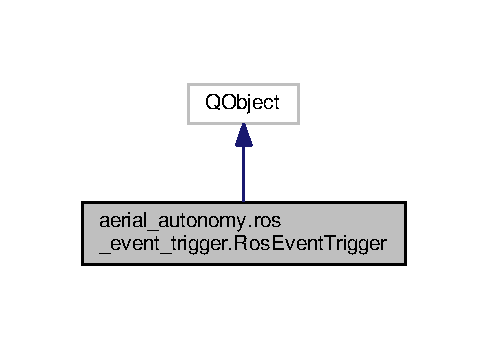
\includegraphics[width=234pt]{classaerial__autonomy_1_1ros__event__trigger_1_1RosEventTrigger__inherit__graph}
\end{center}
\end{figure}


Collaboration diagram for aerial\-\_\-autonomy.\-ros\-\_\-event\-\_\-trigger.\-Ros\-Event\-Trigger\-:\nopagebreak
\begin{figure}[H]
\begin{center}
\leavevmode
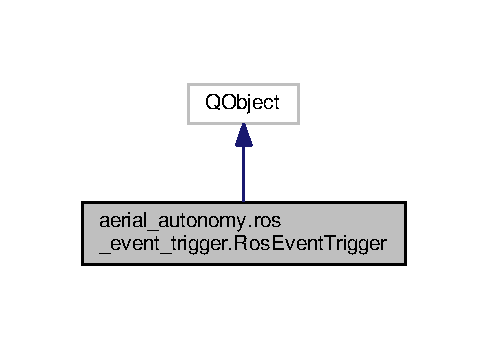
\includegraphics[width=234pt]{classaerial__autonomy_1_1ros__event__trigger_1_1RosEventTrigger__coll__graph}
\end{center}
\end{figure}
\subsection*{Public Member Functions}
\begin{DoxyCompactItemize}
\item 
def \hyperlink{classaerial__autonomy_1_1ros__event__trigger_1_1RosEventTrigger_a740d1aee68ed5c95110242f03ce79e5e}{\-\_\-\-\_\-init\-\_\-\-\_\-}
\begin{DoxyCompactList}\small\item\em Class that loads an event file from a parameter It provides method to trigger\-Events using ros publisher This class separates the G\-U\-I part of plugin from ros interface. \end{DoxyCompactList}\item 
def \hyperlink{classaerial__autonomy_1_1ros__event__trigger_1_1RosEventTrigger_a62ba54708585892d5f227682954fc1c6}{status\-Callback}
\begin{DoxyCompactList}\small\item\em Ros callback for status data from quad, arm, state machine. \end{DoxyCompactList}\item 
def \hyperlink{classaerial__autonomy_1_1ros__event__trigger_1_1RosEventTrigger_a7277f5df8fedc93bf3616535ea588ba8}{trigger\-Pose\-Command}
\begin{DoxyCompactList}\small\item\em Publish pose command event for state machine. \end{DoxyCompactList}\item 
def \hyperlink{classaerial__autonomy_1_1ros__event__trigger_1_1RosEventTrigger_aa7f5a5b057de80bf818642d851fabac3}{trigger\-Event}
\begin{DoxyCompactList}\small\item\em Function to publish ros event based on event name. \end{DoxyCompactList}\end{DoxyCompactItemize}
\subsection*{Public Attributes}
\begin{DoxyCompactItemize}
\item 
\hyperlink{classaerial__autonomy_1_1ros__event__trigger_1_1RosEventTrigger_ac1ff7e7fa3e8ac610473fa8c1e547279}{event\-\_\-manager\-\_\-name}
\begin{DoxyCompactList}\small\item\em Define event manager name. \end{DoxyCompactList}\item 
\hyperlink{classaerial__autonomy_1_1ros__event__trigger_1_1RosEventTrigger_ac24af24de20107643a194072bd64dbd8}{event\-\_\-names\-\_\-list}
\begin{DoxyCompactList}\small\item\em Event names used to create buttons. \end{DoxyCompactList}\item 
\hyperlink{classaerial__autonomy_1_1ros__event__trigger_1_1RosEventTrigger_aa7e45c61e2f9407a82e1e03d83998e6e}{event\-\_\-pub}
\begin{DoxyCompactList}\small\item\em Ros publisher to trigger events based on name. \end{DoxyCompactList}\item 
\hyperlink{classaerial__autonomy_1_1ros__event__trigger_1_1RosEventTrigger_adc9a3f404db853ef8e2b5b988bdaaacb}{pose\-\_\-command\-\_\-pub}
\begin{DoxyCompactList}\small\item\em Ros publisher to trigger pose event. \end{DoxyCompactList}\end{DoxyCompactItemize}
\subsection*{Static Public Attributes}
\begin{DoxyCompactItemize}
\item 
tuple \hyperlink{classaerial__autonomy_1_1ros__event__trigger_1_1RosEventTrigger_ad2e6e150ea166d252a7a40982875fe27}{status\-\_\-signal} = pyqt\-Signal(str, name='system\-Status')
\begin{DoxyCompactList}\small\item\em Send quad sensor/state data as string. \end{DoxyCompactList}\item 
tuple \hyperlink{classaerial__autonomy_1_1ros__event__trigger_1_1RosEventTrigger_a9082897445ba520850cc7108aefe0d77}{pose\-\_\-command\-\_\-signal} = pyqt\-Signal(Pose\-Stamped, name='pose\-Command')
\begin{DoxyCompactList}\small\item\em Send pose command received from Rviz. \end{DoxyCompactList}\end{DoxyCompactItemize}


\subsection{Detailed Description}
Trigger events based on event name. 

Create event name list based on event file 

\subsection{Constructor \& Destructor Documentation}
\hypertarget{classaerial__autonomy_1_1ros__event__trigger_1_1RosEventTrigger_a740d1aee68ed5c95110242f03ce79e5e}{\index{aerial\-\_\-autonomy\-::ros\-\_\-event\-\_\-trigger\-::\-Ros\-Event\-Trigger@{aerial\-\_\-autonomy\-::ros\-\_\-event\-\_\-trigger\-::\-Ros\-Event\-Trigger}!\-\_\-\-\_\-init\-\_\-\-\_\-@{\-\_\-\-\_\-init\-\_\-\-\_\-}}
\index{\-\_\-\-\_\-init\-\_\-\-\_\-@{\-\_\-\-\_\-init\-\_\-\-\_\-}!aerial_autonomy::ros_event_trigger::RosEventTrigger@{aerial\-\_\-autonomy\-::ros\-\_\-event\-\_\-trigger\-::\-Ros\-Event\-Trigger}}
\subsubsection[{\-\_\-\-\_\-init\-\_\-\-\_\-}]{\setlength{\rightskip}{0pt plus 5cm}def aerial\-\_\-autonomy.\-ros\-\_\-event\-\_\-trigger.\-Ros\-Event\-Trigger.\-\_\-\-\_\-init\-\_\-\-\_\- (
\begin{DoxyParamCaption}
\item[{}]{self, }
\item[{}]{event\-\_\-file\-\_\-path}
\end{DoxyParamCaption}
)}}\label{classaerial__autonomy_1_1ros__event__trigger_1_1RosEventTrigger_a740d1aee68ed5c95110242f03ce79e5e}


Class that loads an event file from a parameter It provides method to trigger\-Events using ros publisher This class separates the G\-U\-I part of plugin from ros interface. 



\subsection{Member Function Documentation}
\hypertarget{classaerial__autonomy_1_1ros__event__trigger_1_1RosEventTrigger_a62ba54708585892d5f227682954fc1c6}{\index{aerial\-\_\-autonomy\-::ros\-\_\-event\-\_\-trigger\-::\-Ros\-Event\-Trigger@{aerial\-\_\-autonomy\-::ros\-\_\-event\-\_\-trigger\-::\-Ros\-Event\-Trigger}!status\-Callback@{status\-Callback}}
\index{status\-Callback@{status\-Callback}!aerial_autonomy::ros_event_trigger::RosEventTrigger@{aerial\-\_\-autonomy\-::ros\-\_\-event\-\_\-trigger\-::\-Ros\-Event\-Trigger}}
\subsubsection[{status\-Callback}]{\setlength{\rightskip}{0pt plus 5cm}def aerial\-\_\-autonomy.\-ros\-\_\-event\-\_\-trigger.\-Ros\-Event\-Trigger.\-status\-Callback (
\begin{DoxyParamCaption}
\item[{}]{self, }
\item[{}]{msg, }
\item[{}]{signal}
\end{DoxyParamCaption}
)}}\label{classaerial__autonomy_1_1ros__event__trigger_1_1RosEventTrigger_a62ba54708585892d5f227682954fc1c6}


Ros callback for status data from quad, arm, state machine. 

\hypertarget{classaerial__autonomy_1_1ros__event__trigger_1_1RosEventTrigger_aa7f5a5b057de80bf818642d851fabac3}{\index{aerial\-\_\-autonomy\-::ros\-\_\-event\-\_\-trigger\-::\-Ros\-Event\-Trigger@{aerial\-\_\-autonomy\-::ros\-\_\-event\-\_\-trigger\-::\-Ros\-Event\-Trigger}!trigger\-Event@{trigger\-Event}}
\index{trigger\-Event@{trigger\-Event}!aerial_autonomy::ros_event_trigger::RosEventTrigger@{aerial\-\_\-autonomy\-::ros\-\_\-event\-\_\-trigger\-::\-Ros\-Event\-Trigger}}
\subsubsection[{trigger\-Event}]{\setlength{\rightskip}{0pt plus 5cm}def aerial\-\_\-autonomy.\-ros\-\_\-event\-\_\-trigger.\-Ros\-Event\-Trigger.\-trigger\-Event (
\begin{DoxyParamCaption}
\item[{}]{self, }
\item[{}]{event\-\_\-name}
\end{DoxyParamCaption}
)}}\label{classaerial__autonomy_1_1ros__event__trigger_1_1RosEventTrigger_aa7f5a5b057de80bf818642d851fabac3}


Function to publish ros event based on event name. 

\hypertarget{classaerial__autonomy_1_1ros__event__trigger_1_1RosEventTrigger_a7277f5df8fedc93bf3616535ea588ba8}{\index{aerial\-\_\-autonomy\-::ros\-\_\-event\-\_\-trigger\-::\-Ros\-Event\-Trigger@{aerial\-\_\-autonomy\-::ros\-\_\-event\-\_\-trigger\-::\-Ros\-Event\-Trigger}!trigger\-Pose\-Command@{trigger\-Pose\-Command}}
\index{trigger\-Pose\-Command@{trigger\-Pose\-Command}!aerial_autonomy::ros_event_trigger::RosEventTrigger@{aerial\-\_\-autonomy\-::ros\-\_\-event\-\_\-trigger\-::\-Ros\-Event\-Trigger}}
\subsubsection[{trigger\-Pose\-Command}]{\setlength{\rightskip}{0pt plus 5cm}def aerial\-\_\-autonomy.\-ros\-\_\-event\-\_\-trigger.\-Ros\-Event\-Trigger.\-trigger\-Pose\-Command (
\begin{DoxyParamCaption}
\item[{}]{self, }
\item[{}]{pose}
\end{DoxyParamCaption}
)}}\label{classaerial__autonomy_1_1ros__event__trigger_1_1RosEventTrigger_a7277f5df8fedc93bf3616535ea588ba8}


Publish pose command event for state machine. 



\subsection{Member Data Documentation}
\hypertarget{classaerial__autonomy_1_1ros__event__trigger_1_1RosEventTrigger_ac1ff7e7fa3e8ac610473fa8c1e547279}{\index{aerial\-\_\-autonomy\-::ros\-\_\-event\-\_\-trigger\-::\-Ros\-Event\-Trigger@{aerial\-\_\-autonomy\-::ros\-\_\-event\-\_\-trigger\-::\-Ros\-Event\-Trigger}!event\-\_\-manager\-\_\-name@{event\-\_\-manager\-\_\-name}}
\index{event\-\_\-manager\-\_\-name@{event\-\_\-manager\-\_\-name}!aerial_autonomy::ros_event_trigger::RosEventTrigger@{aerial\-\_\-autonomy\-::ros\-\_\-event\-\_\-trigger\-::\-Ros\-Event\-Trigger}}
\subsubsection[{event\-\_\-manager\-\_\-name}]{\setlength{\rightskip}{0pt plus 5cm}aerial\-\_\-autonomy.\-ros\-\_\-event\-\_\-trigger.\-Ros\-Event\-Trigger.\-event\-\_\-manager\-\_\-name}}\label{classaerial__autonomy_1_1ros__event__trigger_1_1RosEventTrigger_ac1ff7e7fa3e8ac610473fa8c1e547279}


Define event manager name. 

\hypertarget{classaerial__autonomy_1_1ros__event__trigger_1_1RosEventTrigger_ac24af24de20107643a194072bd64dbd8}{\index{aerial\-\_\-autonomy\-::ros\-\_\-event\-\_\-trigger\-::\-Ros\-Event\-Trigger@{aerial\-\_\-autonomy\-::ros\-\_\-event\-\_\-trigger\-::\-Ros\-Event\-Trigger}!event\-\_\-names\-\_\-list@{event\-\_\-names\-\_\-list}}
\index{event\-\_\-names\-\_\-list@{event\-\_\-names\-\_\-list}!aerial_autonomy::ros_event_trigger::RosEventTrigger@{aerial\-\_\-autonomy\-::ros\-\_\-event\-\_\-trigger\-::\-Ros\-Event\-Trigger}}
\subsubsection[{event\-\_\-names\-\_\-list}]{\setlength{\rightskip}{0pt plus 5cm}aerial\-\_\-autonomy.\-ros\-\_\-event\-\_\-trigger.\-Ros\-Event\-Trigger.\-event\-\_\-names\-\_\-list}}\label{classaerial__autonomy_1_1ros__event__trigger_1_1RosEventTrigger_ac24af24de20107643a194072bd64dbd8}


Event names used to create buttons. 

\hypertarget{classaerial__autonomy_1_1ros__event__trigger_1_1RosEventTrigger_aa7e45c61e2f9407a82e1e03d83998e6e}{\index{aerial\-\_\-autonomy\-::ros\-\_\-event\-\_\-trigger\-::\-Ros\-Event\-Trigger@{aerial\-\_\-autonomy\-::ros\-\_\-event\-\_\-trigger\-::\-Ros\-Event\-Trigger}!event\-\_\-pub@{event\-\_\-pub}}
\index{event\-\_\-pub@{event\-\_\-pub}!aerial_autonomy::ros_event_trigger::RosEventTrigger@{aerial\-\_\-autonomy\-::ros\-\_\-event\-\_\-trigger\-::\-Ros\-Event\-Trigger}}
\subsubsection[{event\-\_\-pub}]{\setlength{\rightskip}{0pt plus 5cm}aerial\-\_\-autonomy.\-ros\-\_\-event\-\_\-trigger.\-Ros\-Event\-Trigger.\-event\-\_\-pub}}\label{classaerial__autonomy_1_1ros__event__trigger_1_1RosEventTrigger_aa7e45c61e2f9407a82e1e03d83998e6e}


Ros publisher to trigger events based on name. 

\hypertarget{classaerial__autonomy_1_1ros__event__trigger_1_1RosEventTrigger_adc9a3f404db853ef8e2b5b988bdaaacb}{\index{aerial\-\_\-autonomy\-::ros\-\_\-event\-\_\-trigger\-::\-Ros\-Event\-Trigger@{aerial\-\_\-autonomy\-::ros\-\_\-event\-\_\-trigger\-::\-Ros\-Event\-Trigger}!pose\-\_\-command\-\_\-pub@{pose\-\_\-command\-\_\-pub}}
\index{pose\-\_\-command\-\_\-pub@{pose\-\_\-command\-\_\-pub}!aerial_autonomy::ros_event_trigger::RosEventTrigger@{aerial\-\_\-autonomy\-::ros\-\_\-event\-\_\-trigger\-::\-Ros\-Event\-Trigger}}
\subsubsection[{pose\-\_\-command\-\_\-pub}]{\setlength{\rightskip}{0pt plus 5cm}aerial\-\_\-autonomy.\-ros\-\_\-event\-\_\-trigger.\-Ros\-Event\-Trigger.\-pose\-\_\-command\-\_\-pub}}\label{classaerial__autonomy_1_1ros__event__trigger_1_1RosEventTrigger_adc9a3f404db853ef8e2b5b988bdaaacb}


Ros publisher to trigger pose event. 

\hypertarget{classaerial__autonomy_1_1ros__event__trigger_1_1RosEventTrigger_a9082897445ba520850cc7108aefe0d77}{\index{aerial\-\_\-autonomy\-::ros\-\_\-event\-\_\-trigger\-::\-Ros\-Event\-Trigger@{aerial\-\_\-autonomy\-::ros\-\_\-event\-\_\-trigger\-::\-Ros\-Event\-Trigger}!pose\-\_\-command\-\_\-signal@{pose\-\_\-command\-\_\-signal}}
\index{pose\-\_\-command\-\_\-signal@{pose\-\_\-command\-\_\-signal}!aerial_autonomy::ros_event_trigger::RosEventTrigger@{aerial\-\_\-autonomy\-::ros\-\_\-event\-\_\-trigger\-::\-Ros\-Event\-Trigger}}
\subsubsection[{pose\-\_\-command\-\_\-signal}]{\setlength{\rightskip}{0pt plus 5cm}tuple aerial\-\_\-autonomy.\-ros\-\_\-event\-\_\-trigger.\-Ros\-Event\-Trigger.\-pose\-\_\-command\-\_\-signal = pyqt\-Signal(Pose\-Stamped, name='pose\-Command')\hspace{0.3cm}{\ttfamily [static]}}}\label{classaerial__autonomy_1_1ros__event__trigger_1_1RosEventTrigger_a9082897445ba520850cc7108aefe0d77}


Send pose command received from Rviz. 

\hypertarget{classaerial__autonomy_1_1ros__event__trigger_1_1RosEventTrigger_ad2e6e150ea166d252a7a40982875fe27}{\index{aerial\-\_\-autonomy\-::ros\-\_\-event\-\_\-trigger\-::\-Ros\-Event\-Trigger@{aerial\-\_\-autonomy\-::ros\-\_\-event\-\_\-trigger\-::\-Ros\-Event\-Trigger}!status\-\_\-signal@{status\-\_\-signal}}
\index{status\-\_\-signal@{status\-\_\-signal}!aerial_autonomy::ros_event_trigger::RosEventTrigger@{aerial\-\_\-autonomy\-::ros\-\_\-event\-\_\-trigger\-::\-Ros\-Event\-Trigger}}
\subsubsection[{status\-\_\-signal}]{\setlength{\rightskip}{0pt plus 5cm}tuple aerial\-\_\-autonomy.\-ros\-\_\-event\-\_\-trigger.\-Ros\-Event\-Trigger.\-status\-\_\-signal = pyqt\-Signal(str, name='system\-Status')\hspace{0.3cm}{\ttfamily [static]}}}\label{classaerial__autonomy_1_1ros__event__trigger_1_1RosEventTrigger_ad2e6e150ea166d252a7a40982875fe27}


Send quad sensor/state data as string. 



The documentation for this class was generated from the following file\-:\begin{DoxyCompactItemize}
\item 
src/aerial\-\_\-autonomy/\hyperlink{ros__event__trigger_8py}{ros\-\_\-event\-\_\-trigger.\-py}\end{DoxyCompactItemize}

\hypertarget{classSampleLogicStateMachine__}{\section{Sample\-Logic\-State\-Machine\-\_\-$<$ Robot\-System\-T $>$ Class Template Reference}
\label{classSampleLogicStateMachine__}\index{Sample\-Logic\-State\-Machine\-\_\-$<$ Robot\-System\-T $>$@{Sample\-Logic\-State\-Machine\-\_\-$<$ Robot\-System\-T $>$}}
}


Example Logic state machine that stores triggered event.  




{\ttfamily \#include $<$sample\-\_\-logic\-\_\-state\-\_\-machine.\-h$>$}

\subsection*{Public Member Functions}
\begin{DoxyCompactItemize}
\item 
\hyperlink{classSampleLogicStateMachine___a5450901d1fdbedd6368ea302322a5fb6}{Sample\-Logic\-State\-Machine\-\_\-} (Robot\-System\-T \&robot\-\_\-system)
\begin{DoxyCompactList}\small\item\em Constructor that takes robot system. \end{DoxyCompactList}\item 
{\footnotesize template$<$class Event $>$ }\\void \hyperlink{classSampleLogicStateMachine___af577b426ec630d48148ed6aab393b43e}{process\-\_\-event} (const Event \&event)
\begin{DoxyCompactList}\small\item\em Generic process event that stores the event type. \end{DoxyCompactList}\item 
void \hyperlink{classSampleLogicStateMachine___a60ca43f8a484f1ab56669d0485479c47}{process\-\_\-event} (const \hyperlink{structPositionYaw}{Position\-Yaw} \&event)
\begin{DoxyCompactList}\small\item\em process pose event message \end{DoxyCompactList}\item 
std\-::type\-\_\-index \hyperlink{classSampleLogicStateMachine___a469a3cdffcce57a12c5b7890410b63e8}{get\-Process\-Event\-Type\-Id} ()
\begin{DoxyCompactList}\small\item\em retrieve the event type\-\_\-index of last processed event \end{DoxyCompactList}\item 
\hyperlink{structPositionYaw}{Position\-Yaw} \hyperlink{classSampleLogicStateMachine___a254ed914235117e9ffaa5ba8614335cb}{get\-Pose\-Event} ()
\begin{DoxyCompactList}\small\item\em retrieve poseyaw event message \end{DoxyCompactList}\end{DoxyCompactItemize}
\subsection*{Friends}
\begin{DoxyCompactItemize}
\item 
{\footnotesize template$<$class Event\-T , class Robot\-System\-T1 , class Logic\-State\-Machine\-T $>$ }\\class \hyperlink{classSampleLogicStateMachine___a05673eb4ec343f36c1f3fb787ac26b94}{Action\-Functor}
\begin{DoxyCompactList}\small\item\em Friend action class to guard robot system. \end{DoxyCompactList}\item 
{\footnotesize template$<$class Event\-T , class Robot\-System\-T1 , class Logic\-State\-Machine\-T $>$ }\\class \hyperlink{classSampleLogicStateMachine___a9411581bb37b54467df520e3c73ceaf0}{Guard\-Functor}
\begin{DoxyCompactList}\small\item\em Friend guard class to access robot system. \end{DoxyCompactList}\item 
{\footnotesize template$<$class Robot\-System\-T1 , class Logic\-State\-Machine\-T $>$ }\\class \hyperlink{classSampleLogicStateMachine___a86a665e36420c3cbc2b45864e023f98a}{Event\-Agnostic\-Action\-Functor}
\begin{DoxyCompactList}\small\item\em Frient Event agnostic action class. \end{DoxyCompactList}\item 
{\footnotesize template$<$class Robot\-System\-T1 , class Logic\-State\-Machine\-T $>$ }\\class \hyperlink{classSampleLogicStateMachine___af372c36475bc4510af791f5cb66608ad}{Event\-Agnostic\-Guard\-Functor}
\begin{DoxyCompactList}\small\item\em Frient Event agnostic guard class. \end{DoxyCompactList}\end{DoxyCompactItemize}


\subsection{Detailed Description}
\subsubsection*{template$<$class Robot\-System\-T$>$class Sample\-Logic\-State\-Machine\-\_\-$<$ Robot\-System\-T $>$}

Example Logic state machine that stores triggered event. 


\begin{DoxyTemplParams}{Template Parameters}
{\em Robot\-System\-T} & The robot system that is used by states to perform actions \\
\hline
\end{DoxyTemplParams}


\subsection{Constructor \& Destructor Documentation}
\hypertarget{classSampleLogicStateMachine___a5450901d1fdbedd6368ea302322a5fb6}{\index{Sample\-Logic\-State\-Machine\-\_\-@{Sample\-Logic\-State\-Machine\-\_\-}!Sample\-Logic\-State\-Machine\-\_\-@{Sample\-Logic\-State\-Machine\-\_\-}}
\index{Sample\-Logic\-State\-Machine\-\_\-@{Sample\-Logic\-State\-Machine\-\_\-}!SampleLogicStateMachine_@{Sample\-Logic\-State\-Machine\-\_\-}}
\subsubsection[{Sample\-Logic\-State\-Machine\-\_\-}]{\setlength{\rightskip}{0pt plus 5cm}template$<$class Robot\-System\-T $>$ {\bf Sample\-Logic\-State\-Machine\-\_\-}$<$ Robot\-System\-T $>$\-::{\bf Sample\-Logic\-State\-Machine\-\_\-} (
\begin{DoxyParamCaption}
\item[{Robot\-System\-T \&}]{robot\-\_\-system}
\end{DoxyParamCaption}
)\hspace{0.3cm}{\ttfamily [inline]}}}\label{classSampleLogicStateMachine___a5450901d1fdbedd6368ea302322a5fb6}


Constructor that takes robot system. 


\begin{DoxyParams}{Parameters}
{\em robot\-\_\-system} & provides actions to select controllers, get/set Goals. \\
\hline
\end{DoxyParams}


\subsection{Member Function Documentation}
\hypertarget{classSampleLogicStateMachine___a254ed914235117e9ffaa5ba8614335cb}{\index{Sample\-Logic\-State\-Machine\-\_\-@{Sample\-Logic\-State\-Machine\-\_\-}!get\-Pose\-Event@{get\-Pose\-Event}}
\index{get\-Pose\-Event@{get\-Pose\-Event}!SampleLogicStateMachine_@{Sample\-Logic\-State\-Machine\-\_\-}}
\subsubsection[{get\-Pose\-Event}]{\setlength{\rightskip}{0pt plus 5cm}template$<$class Robot\-System\-T $>$ {\bf Position\-Yaw} {\bf Sample\-Logic\-State\-Machine\-\_\-}$<$ Robot\-System\-T $>$\-::get\-Pose\-Event (
\begin{DoxyParamCaption}
{}
\end{DoxyParamCaption}
)\hspace{0.3cm}{\ttfamily [inline]}}}\label{classSampleLogicStateMachine___a254ed914235117e9ffaa5ba8614335cb}


retrieve poseyaw event message 

\begin{DoxyReturn}{Returns}
poseyaw event message 
\end{DoxyReturn}
\hypertarget{classSampleLogicStateMachine___a469a3cdffcce57a12c5b7890410b63e8}{\index{Sample\-Logic\-State\-Machine\-\_\-@{Sample\-Logic\-State\-Machine\-\_\-}!get\-Process\-Event\-Type\-Id@{get\-Process\-Event\-Type\-Id}}
\index{get\-Process\-Event\-Type\-Id@{get\-Process\-Event\-Type\-Id}!SampleLogicStateMachine_@{Sample\-Logic\-State\-Machine\-\_\-}}
\subsubsection[{get\-Process\-Event\-Type\-Id}]{\setlength{\rightskip}{0pt plus 5cm}template$<$class Robot\-System\-T $>$ std\-::type\-\_\-index {\bf Sample\-Logic\-State\-Machine\-\_\-}$<$ Robot\-System\-T $>$\-::get\-Process\-Event\-Type\-Id (
\begin{DoxyParamCaption}
{}
\end{DoxyParamCaption}
)\hspace{0.3cm}{\ttfamily [inline]}}}\label{classSampleLogicStateMachine___a469a3cdffcce57a12c5b7890410b63e8}


retrieve the event type\-\_\-index of last processed event 

\begin{DoxyReturn}{Returns}
type\-\_\-index of the last processed event 
\end{DoxyReturn}
\hypertarget{classSampleLogicStateMachine___af577b426ec630d48148ed6aab393b43e}{\index{Sample\-Logic\-State\-Machine\-\_\-@{Sample\-Logic\-State\-Machine\-\_\-}!process\-\_\-event@{process\-\_\-event}}
\index{process\-\_\-event@{process\-\_\-event}!SampleLogicStateMachine_@{Sample\-Logic\-State\-Machine\-\_\-}}
\subsubsection[{process\-\_\-event}]{\setlength{\rightskip}{0pt plus 5cm}template$<$class Robot\-System\-T $>$ template$<$class Event $>$ void {\bf Sample\-Logic\-State\-Machine\-\_\-}$<$ Robot\-System\-T $>$\-::process\-\_\-event (
\begin{DoxyParamCaption}
\item[{const Event \&}]{event}
\end{DoxyParamCaption}
)\hspace{0.3cm}{\ttfamily [inline]}}}\label{classSampleLogicStateMachine___af577b426ec630d48148ed6aab393b43e}


Generic process event that stores the event type. 


\begin{DoxyTemplParams}{Template Parameters}
{\em Event} & Event type \\
\hline
\end{DoxyTemplParams}

\begin{DoxyParams}{Parameters}
{\em event} & Event instance sent in to process \\
\hline
\end{DoxyParams}
\hypertarget{classSampleLogicStateMachine___a60ca43f8a484f1ab56669d0485479c47}{\index{Sample\-Logic\-State\-Machine\-\_\-@{Sample\-Logic\-State\-Machine\-\_\-}!process\-\_\-event@{process\-\_\-event}}
\index{process\-\_\-event@{process\-\_\-event}!SampleLogicStateMachine_@{Sample\-Logic\-State\-Machine\-\_\-}}
\subsubsection[{process\-\_\-event}]{\setlength{\rightskip}{0pt plus 5cm}template$<$class Robot\-System\-T $>$ void {\bf Sample\-Logic\-State\-Machine\-\_\-}$<$ Robot\-System\-T $>$\-::process\-\_\-event (
\begin{DoxyParamCaption}
\item[{const {\bf Position\-Yaw} \&}]{event}
\end{DoxyParamCaption}
)\hspace{0.3cm}{\ttfamily [inline]}}}\label{classSampleLogicStateMachine___a60ca43f8a484f1ab56669d0485479c47}


process pose event message 


\begin{DoxyParams}{Parameters}
{\em event} & message that is stored \\
\hline
\end{DoxyParams}


\subsection{Friends And Related Function Documentation}
\hypertarget{classSampleLogicStateMachine___a05673eb4ec343f36c1f3fb787ac26b94}{\index{Sample\-Logic\-State\-Machine\-\_\-@{Sample\-Logic\-State\-Machine\-\_\-}!Action\-Functor@{Action\-Functor}}
\index{Action\-Functor@{Action\-Functor}!SampleLogicStateMachine_@{Sample\-Logic\-State\-Machine\-\_\-}}
\subsubsection[{Action\-Functor}]{\setlength{\rightskip}{0pt plus 5cm}template$<$class Robot\-System\-T $>$ template$<$class Event\-T , class Robot\-System\-T1 , class Logic\-State\-Machine\-T $>$ friend class {\bf Action\-Functor}\hspace{0.3cm}{\ttfamily [friend]}}}\label{classSampleLogicStateMachine___a05673eb4ec343f36c1f3fb787ac26b94}


Friend action class to guard robot system. 


\begin{DoxyTemplParams}{Template Parameters}
{\em Event\-T} & Event triggering action functor \\
\hline
{\em Robot\-System\-T1} & Robot system used by action functor \\
\hline
{\em Logic\-State\-Machine\-T} & Logic state Machine backend used by Guard functor \\
\hline
\end{DoxyTemplParams}
\hypertarget{classSampleLogicStateMachine___a86a665e36420c3cbc2b45864e023f98a}{\index{Sample\-Logic\-State\-Machine\-\_\-@{Sample\-Logic\-State\-Machine\-\_\-}!Event\-Agnostic\-Action\-Functor@{Event\-Agnostic\-Action\-Functor}}
\index{Event\-Agnostic\-Action\-Functor@{Event\-Agnostic\-Action\-Functor}!SampleLogicStateMachine_@{Sample\-Logic\-State\-Machine\-\_\-}}
\subsubsection[{Event\-Agnostic\-Action\-Functor}]{\setlength{\rightskip}{0pt plus 5cm}template$<$class Robot\-System\-T $>$ template$<$class Robot\-System\-T1 , class Logic\-State\-Machine\-T $>$ friend class {\bf Event\-Agnostic\-Action\-Functor}\hspace{0.3cm}{\ttfamily [friend]}}}\label{classSampleLogicStateMachine___a86a665e36420c3cbc2b45864e023f98a}


Frient Event agnostic action class. 


\begin{DoxyTemplParams}{Template Parameters}
{\em Event\-T} & Event triggering action functor \\
\hline
{\em Robot\-System\-T1} & Robot system used by action functor \\
\hline
{\em Logic\-State\-Machine\-T} & Logic state Machine backend used by Guard functor \\
\hline
\end{DoxyTemplParams}
\hypertarget{classSampleLogicStateMachine___af372c36475bc4510af791f5cb66608ad}{\index{Sample\-Logic\-State\-Machine\-\_\-@{Sample\-Logic\-State\-Machine\-\_\-}!Event\-Agnostic\-Guard\-Functor@{Event\-Agnostic\-Guard\-Functor}}
\index{Event\-Agnostic\-Guard\-Functor@{Event\-Agnostic\-Guard\-Functor}!SampleLogicStateMachine_@{Sample\-Logic\-State\-Machine\-\_\-}}
\subsubsection[{Event\-Agnostic\-Guard\-Functor}]{\setlength{\rightskip}{0pt plus 5cm}template$<$class Robot\-System\-T $>$ template$<$class Robot\-System\-T1 , class Logic\-State\-Machine\-T $>$ friend class {\bf Event\-Agnostic\-Guard\-Functor}\hspace{0.3cm}{\ttfamily [friend]}}}\label{classSampleLogicStateMachine___af372c36475bc4510af791f5cb66608ad}


Frient Event agnostic guard class. 


\begin{DoxyTemplParams}{Template Parameters}
{\em Event\-T} & Event triggering action functor \\
\hline
{\em Robot\-System\-T1} & Robot system used by action functor \\
\hline
{\em Logic\-State\-Machine\-T} & Logic state Machine backend used by Guard functor \\
\hline
\end{DoxyTemplParams}
\hypertarget{classSampleLogicStateMachine___a9411581bb37b54467df520e3c73ceaf0}{\index{Sample\-Logic\-State\-Machine\-\_\-@{Sample\-Logic\-State\-Machine\-\_\-}!Guard\-Functor@{Guard\-Functor}}
\index{Guard\-Functor@{Guard\-Functor}!SampleLogicStateMachine_@{Sample\-Logic\-State\-Machine\-\_\-}}
\subsubsection[{Guard\-Functor}]{\setlength{\rightskip}{0pt plus 5cm}template$<$class Robot\-System\-T $>$ template$<$class Event\-T , class Robot\-System\-T1 , class Logic\-State\-Machine\-T $>$ friend class {\bf Guard\-Functor}\hspace{0.3cm}{\ttfamily [friend]}}}\label{classSampleLogicStateMachine___a9411581bb37b54467df520e3c73ceaf0}


Friend guard class to access robot system. 


\begin{DoxyTemplParams}{Template Parameters}
{\em Event\-T} & Event triggering action functor \\
\hline
{\em Robot\-System\-T1} & Robot system used by action functor \\
\hline
{\em Logic\-State\-Machine\-T} & Logic state Machine backend used by Guard functor \\
\hline
\end{DoxyTemplParams}


The documentation for this class was generated from the following file\-:\begin{DoxyCompactItemize}
\item 
include/aerial\-\_\-autonomy/tests/\hyperlink{sample__logic__state__machine_8h}{sample\-\_\-logic\-\_\-state\-\_\-machine.\-h}\end{DoxyCompactItemize}

\hypertarget{classSampleParser}{\section{Sample\-Parser Class Reference}
\label{classSampleParser}\index{Sample\-Parser@{Sample\-Parser}}
}


An example U\-A\-V hardware that emulates actual U\-A\-V hardware.  




{\ttfamily \#include $<$sample\-\_\-parser.\-h$>$}



Inheritance diagram for Sample\-Parser\-:\nopagebreak
\begin{figure}[H]
\begin{center}
\leavevmode
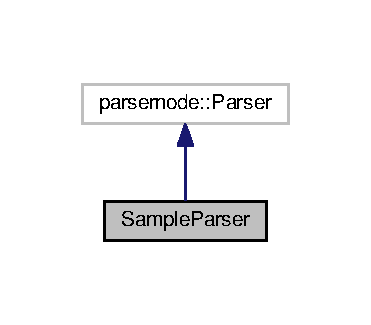
\includegraphics[width=178pt]{classSampleParser__inherit__graph}
\end{center}
\end{figure}


Collaboration diagram for Sample\-Parser\-:\nopagebreak
\begin{figure}[H]
\begin{center}
\leavevmode
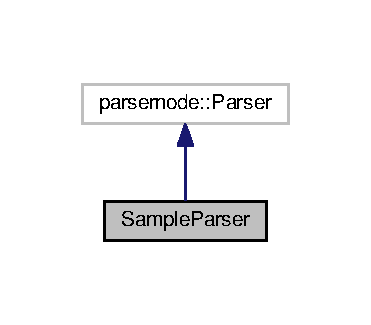
\includegraphics[width=178pt]{classSampleParser__coll__graph}
\end{center}
\end{figure}
\subsection*{Public Member Functions}
\begin{DoxyCompactItemize}
\item 
\hyperlink{classSampleParser_a8cea9add13717649b00c4e916fe3b518}{Sample\-Parser} ()
\begin{DoxyCompactList}\small\item\em Implict constructor. \end{DoxyCompactList}\item 
void \hyperlink{classSampleParser_a50ed35fede29930ff853fe6ab175fad6}{set\-R\-C} (int16\-\_\-t channels\mbox{[}4\mbox{]})
\begin{DoxyCompactList}\small\item\em set the rc channel information stored in the U\-A\-V brain \end{DoxyCompactList}\item 
virtual bool \hyperlink{classSampleParser_aaec0124f3a5a19e183438484f98db761}{takeoff} ()
\begin{DoxyCompactList}\small\item\em Takeoff. \end{DoxyCompactList}\item 
virtual bool \hyperlink{classSampleParser_a92ee9e3720b7c420714e2904f81a113a}{land} ()
\begin{DoxyCompactList}\small\item\em Land. \end{DoxyCompactList}\item 
virtual bool \hyperlink{classSampleParser_ad057bfe380db45cda437f53cec2c267a}{disarm} ()
\begin{DoxyCompactList}\small\item\em Turn off motor. \end{DoxyCompactList}\item 
virtual bool \hyperlink{classSampleParser_a265b674d9c0467ed919cff3f4df803b5}{flow\-Control} (bool)
\begin{DoxyCompactList}\small\item\em Toggle software control. \end{DoxyCompactList}\item 
virtual bool \hyperlink{classSampleParser_abb19d034c771cbd02d1961d99ca35f98}{calibrateimubias} ()
\begin{DoxyCompactList}\small\item\em Recalibrate I\-M\-U. \end{DoxyCompactList}\item 
virtual bool \hyperlink{classSampleParser_a95c4ea3034bcd431660f5ee2acc13e3c}{cmdrpythrust} (geometry\-\_\-msgs\-::\-Quaternion \&rpytmsg, bool sendyaw=false)
\begin{DoxyCompactList}\small\item\em Command the euler angles of the quad and the thrust. \end{DoxyCompactList}\item 
virtual bool \hyperlink{classSampleParser_a52ea7095057fa73ae1665a8dd6ccd0d0}{cmdvelguided} (geometry\-\_\-msgs\-::\-Vector3 \&vel\-\_\-cmd, double \&yaw\-\_\-ang)
\begin{DoxyCompactList}\small\item\em Command velocity and yaw to U\-A\-V. \end{DoxyCompactList}\item 
virtual bool \hyperlink{classSampleParser_a790a0041665973477028493cf51b8059}{cmdwaypoint} (geometry\-\_\-msgs\-::\-Vector3 \&desired\-\_\-pos, double desired\-\_\-yaw=0)
\begin{DoxyCompactList}\small\item\em Command position yaw for U\-A\-V. \end{DoxyCompactList}\item 
virtual void \hyperlink{classSampleParser_a20f989659a8d7d65574d37460a1e9f47}{grip} (int state)
\begin{DoxyCompactList}\small\item\em Toggle gripper. \end{DoxyCompactList}\item 
virtual void \hyperlink{classSampleParser_ab062fe44a82f5490e5c92e8512ede9a2}{reset\-\_\-attitude} (double roll, double pitch, double yaw)
\begin{DoxyCompactList}\small\item\em Set the attitude data to specified roll, pitch, yaw (rad) \end{DoxyCompactList}\item 
virtual void \hyperlink{classSampleParser_a955965dff0214bbb8e720cab858f1078}{setmode} (std\-::string mode)
\begin{DoxyCompactList}\small\item\em Set U\-A\-V controller mode such position controlling, rpyt etc. \end{DoxyCompactList}\item 
virtual void \hyperlink{classSampleParser_acaf99fced8fc57433781e766dcb931cf}{initialize} (ros\-::\-Node\-Handle \&nh\-\_\-)
\begin{DoxyCompactList}\small\item\em Initialize the Hardware with a ros node handle to setup communications. \end{DoxyCompactList}\item 
virtual void \hyperlink{classSampleParser_af1be68e602c959d8b1ab29d651ed379c}{getquaddata} (parsernode\-::common\-::quaddata \&d1)
\begin{DoxyCompactList}\small\item\em Get the sensor data and U\-A\-V state. \end{DoxyCompactList}\item 
virtual \hyperlink{classSampleParser_afc4af7450f685341c09e2c00af95ff73}{$\sim$\-Sample\-Parser} ()
\begin{DoxyCompactList}\small\item\em Polymorphic destructor. \end{DoxyCompactList}\item 
virtual void \hyperlink{classSampleParser_a293772680222eb4f7c49c26d42e69eaa}{set\-Battery\-Percent} (double percent)
\begin{DoxyCompactList}\small\item\em Set the battery percent sensor data. \end{DoxyCompactList}\item 
virtual void \hyperlink{classSampleParser_a98153bd7644b1ca0eb12b442ec54034f}{setaltitude} (double altitude\-\_\-)
\begin{DoxyCompactList}\small\item\em set the altitude or local z height data(m) \end{DoxyCompactList}\item 
virtual void \hyperlink{classSampleParser_aaf4d068b2dabd1ca8da12f7109b288c4}{setlogdir} (string logdir)
\begin{DoxyCompactList}\small\item\em Create log directory and create log files. \end{DoxyCompactList}\item 
virtual void \hyperlink{classSampleParser_a78923bbce68debb4d035a2d8b25f7d6d}{controllog} (bool logswitch)
\begin{DoxyCompactList}\small\item\em Toggle logging. \end{DoxyCompactList}\end{DoxyCompactItemize}


\subsection{Detailed Description}
An example U\-A\-V hardware that emulates actual U\-A\-V hardware. 

\subsection{Constructor \& Destructor Documentation}
\hypertarget{classSampleParser_a8cea9add13717649b00c4e916fe3b518}{\index{Sample\-Parser@{Sample\-Parser}!Sample\-Parser@{Sample\-Parser}}
\index{Sample\-Parser@{Sample\-Parser}!SampleParser@{Sample\-Parser}}
\subsubsection[{Sample\-Parser}]{\setlength{\rightskip}{0pt plus 5cm}Sample\-Parser\-::\-Sample\-Parser (
\begin{DoxyParamCaption}
{}
\end{DoxyParamCaption}
)\hspace{0.3cm}{\ttfamily [inline]}}}\label{classSampleParser_a8cea9add13717649b00c4e916fe3b518}


Implict constructor. 

\hypertarget{classSampleParser_afc4af7450f685341c09e2c00af95ff73}{\index{Sample\-Parser@{Sample\-Parser}!$\sim$\-Sample\-Parser@{$\sim$\-Sample\-Parser}}
\index{$\sim$\-Sample\-Parser@{$\sim$\-Sample\-Parser}!SampleParser@{Sample\-Parser}}
\subsubsection[{$\sim$\-Sample\-Parser}]{\setlength{\rightskip}{0pt plus 5cm}virtual Sample\-Parser\-::$\sim$\-Sample\-Parser (
\begin{DoxyParamCaption}
{}
\end{DoxyParamCaption}
)\hspace{0.3cm}{\ttfamily [inline]}, {\ttfamily [virtual]}}}\label{classSampleParser_afc4af7450f685341c09e2c00af95ff73}


Polymorphic destructor. 



\subsection{Member Function Documentation}
\hypertarget{classSampleParser_abb19d034c771cbd02d1961d99ca35f98}{\index{Sample\-Parser@{Sample\-Parser}!calibrateimubias@{calibrateimubias}}
\index{calibrateimubias@{calibrateimubias}!SampleParser@{Sample\-Parser}}
\subsubsection[{calibrateimubias}]{\setlength{\rightskip}{0pt plus 5cm}virtual bool Sample\-Parser\-::calibrateimubias (
\begin{DoxyParamCaption}
{}
\end{DoxyParamCaption}
)\hspace{0.3cm}{\ttfamily [inline]}, {\ttfamily [virtual]}}}\label{classSampleParser_abb19d034c771cbd02d1961d99ca35f98}


Recalibrate I\-M\-U. 

\begin{DoxyReturn}{Returns}
true if calibration successful 
\end{DoxyReturn}
\hypertarget{classSampleParser_a95c4ea3034bcd431660f5ee2acc13e3c}{\index{Sample\-Parser@{Sample\-Parser}!cmdrpythrust@{cmdrpythrust}}
\index{cmdrpythrust@{cmdrpythrust}!SampleParser@{Sample\-Parser}}
\subsubsection[{cmdrpythrust}]{\setlength{\rightskip}{0pt plus 5cm}virtual bool Sample\-Parser\-::cmdrpythrust (
\begin{DoxyParamCaption}
\item[{geometry\-\_\-msgs\-::\-Quaternion \&}]{rpytmsg, }
\item[{bool}]{sendyaw = {\ttfamily false}}
\end{DoxyParamCaption}
)\hspace{0.3cm}{\ttfamily [inline]}, {\ttfamily [virtual]}}}\label{classSampleParser_a95c4ea3034bcd431660f5ee2acc13e3c}


Command the euler angles of the quad and the thrust. 


\begin{DoxyParams}{Parameters}
{\em rpytmsg} & Msg format is (x,y,z,w) -\/$>$ (roll, pitch, yaw, thrust). The thrust value will be adjusted based on whethere there is thrust bias or not. \\
\hline
{\em sendyaw} & True to control the yaw/ False to ignore yaw command\\
\hline
\end{DoxyParams}
\begin{DoxyReturn}{Returns}
True if sending command is successful 
\end{DoxyReturn}
\hypertarget{classSampleParser_a52ea7095057fa73ae1665a8dd6ccd0d0}{\index{Sample\-Parser@{Sample\-Parser}!cmdvelguided@{cmdvelguided}}
\index{cmdvelguided@{cmdvelguided}!SampleParser@{Sample\-Parser}}
\subsubsection[{cmdvelguided}]{\setlength{\rightskip}{0pt plus 5cm}virtual bool Sample\-Parser\-::cmdvelguided (
\begin{DoxyParamCaption}
\item[{geometry\-\_\-msgs\-::\-Vector3 \&}]{vel\-\_\-cmd, }
\item[{double \&}]{yaw\-\_\-ang}
\end{DoxyParamCaption}
)\hspace{0.3cm}{\ttfamily [inline]}, {\ttfamily [virtual]}}}\label{classSampleParser_a52ea7095057fa73ae1665a8dd6ccd0d0}


Command velocity and yaw to U\-A\-V. 


\begin{DoxyParams}{Parameters}
{\em vel\-\_\-cmd} & \hyperlink{structVelocity}{Velocity} vector (m/s) \\
\hline
{\em yaw\-\_\-ang} & Yaw angle (rad)\\
\hline
\end{DoxyParams}
\begin{DoxyReturn}{Returns}
True if sending command is successful 
\end{DoxyReturn}
\hypertarget{classSampleParser_a790a0041665973477028493cf51b8059}{\index{Sample\-Parser@{Sample\-Parser}!cmdwaypoint@{cmdwaypoint}}
\index{cmdwaypoint@{cmdwaypoint}!SampleParser@{Sample\-Parser}}
\subsubsection[{cmdwaypoint}]{\setlength{\rightskip}{0pt plus 5cm}virtual bool Sample\-Parser\-::cmdwaypoint (
\begin{DoxyParamCaption}
\item[{geometry\-\_\-msgs\-::\-Vector3 \&}]{desired\-\_\-pos, }
\item[{double}]{desired\-\_\-yaw = {\ttfamily 0}}
\end{DoxyParamCaption}
)\hspace{0.3cm}{\ttfamily [inline]}, {\ttfamily [virtual]}}}\label{classSampleParser_a790a0041665973477028493cf51b8059}


Command position yaw for U\-A\-V. 


\begin{DoxyParams}{Parameters}
{\em desired\-\_\-pos} & Desired 3\-D position (m) \\
\hline
{\em desired\-\_\-yaw} & Desired yaw angle (rad)\\
\hline
\end{DoxyParams}
\begin{DoxyReturn}{Returns}
True if sending command is successful 
\end{DoxyReturn}
\hypertarget{classSampleParser_a78923bbce68debb4d035a2d8b25f7d6d}{\index{Sample\-Parser@{Sample\-Parser}!controllog@{controllog}}
\index{controllog@{controllog}!SampleParser@{Sample\-Parser}}
\subsubsection[{controllog}]{\setlength{\rightskip}{0pt plus 5cm}virtual void Sample\-Parser\-::controllog (
\begin{DoxyParamCaption}
\item[{bool}]{logswitch}
\end{DoxyParamCaption}
)\hspace{0.3cm}{\ttfamily [inline]}, {\ttfamily [virtual]}}}\label{classSampleParser_a78923bbce68debb4d035a2d8b25f7d6d}


Toggle logging. 


\begin{DoxyParams}{Parameters}
{\em logswitch} & True to start logging/\-False to stop logging \\
\hline
\end{DoxyParams}
\hypertarget{classSampleParser_ad057bfe380db45cda437f53cec2c267a}{\index{Sample\-Parser@{Sample\-Parser}!disarm@{disarm}}
\index{disarm@{disarm}!SampleParser@{Sample\-Parser}}
\subsubsection[{disarm}]{\setlength{\rightskip}{0pt plus 5cm}virtual bool Sample\-Parser\-::disarm (
\begin{DoxyParamCaption}
{}
\end{DoxyParamCaption}
)\hspace{0.3cm}{\ttfamily [inline]}, {\ttfamily [virtual]}}}\label{classSampleParser_ad057bfe380db45cda437f53cec2c267a}


Turn off motor. 

\begin{DoxyReturn}{Returns}
True if disabling is successful 
\end{DoxyReturn}
\hypertarget{classSampleParser_a265b674d9c0467ed919cff3f4df803b5}{\index{Sample\-Parser@{Sample\-Parser}!flow\-Control@{flow\-Control}}
\index{flow\-Control@{flow\-Control}!SampleParser@{Sample\-Parser}}
\subsubsection[{flow\-Control}]{\setlength{\rightskip}{0pt plus 5cm}virtual bool Sample\-Parser\-::flow\-Control (
\begin{DoxyParamCaption}
\item[{bool}]{}
\end{DoxyParamCaption}
)\hspace{0.3cm}{\ttfamily [inline]}, {\ttfamily [virtual]}}}\label{classSampleParser_a265b674d9c0467ed919cff3f4df803b5}


Toggle software control. 

\begin{DoxyReturn}{Returns}
True if successful 
\end{DoxyReturn}
\hypertarget{classSampleParser_af1be68e602c959d8b1ab29d651ed379c}{\index{Sample\-Parser@{Sample\-Parser}!getquaddata@{getquaddata}}
\index{getquaddata@{getquaddata}!SampleParser@{Sample\-Parser}}
\subsubsection[{getquaddata}]{\setlength{\rightskip}{0pt plus 5cm}virtual void Sample\-Parser\-::getquaddata (
\begin{DoxyParamCaption}
\item[{parsernode\-::common\-::quaddata \&}]{d1}
\end{DoxyParamCaption}
)\hspace{0.3cm}{\ttfamily [inline]}, {\ttfamily [virtual]}}}\label{classSampleParser_af1be68e602c959d8b1ab29d651ed379c}


Get the sensor data and U\-A\-V state. 


\begin{DoxyParams}{Parameters}
{\em d1} & Data struct in which data is filled \\
\hline
\end{DoxyParams}
\hypertarget{classSampleParser_a20f989659a8d7d65574d37460a1e9f47}{\index{Sample\-Parser@{Sample\-Parser}!grip@{grip}}
\index{grip@{grip}!SampleParser@{Sample\-Parser}}
\subsubsection[{grip}]{\setlength{\rightskip}{0pt plus 5cm}virtual void Sample\-Parser\-::grip (
\begin{DoxyParamCaption}
\item[{int}]{state}
\end{DoxyParamCaption}
)\hspace{0.3cm}{\ttfamily [inline]}, {\ttfamily [virtual]}}}\label{classSampleParser_a20f989659a8d7d65574d37460a1e9f47}


Toggle gripper. 


\begin{DoxyParams}{Parameters}
{\em state} & 0 to close, 1 to open \\
\hline
\end{DoxyParams}
\hypertarget{classSampleParser_acaf99fced8fc57433781e766dcb931cf}{\index{Sample\-Parser@{Sample\-Parser}!initialize@{initialize}}
\index{initialize@{initialize}!SampleParser@{Sample\-Parser}}
\subsubsection[{initialize}]{\setlength{\rightskip}{0pt plus 5cm}virtual void Sample\-Parser\-::initialize (
\begin{DoxyParamCaption}
\item[{ros\-::\-Node\-Handle \&}]{nh\-\_\-}
\end{DoxyParamCaption}
)\hspace{0.3cm}{\ttfamily [inline]}, {\ttfamily [virtual]}}}\label{classSampleParser_acaf99fced8fc57433781e766dcb931cf}


Initialize the Hardware with a ros node handle to setup communications. 


\begin{DoxyParams}{Parameters}
{\em nh\-\_\-} & Nodehandle to setup communications \\
\hline
\end{DoxyParams}
\hypertarget{classSampleParser_a92ee9e3720b7c420714e2904f81a113a}{\index{Sample\-Parser@{Sample\-Parser}!land@{land}}
\index{land@{land}!SampleParser@{Sample\-Parser}}
\subsubsection[{land}]{\setlength{\rightskip}{0pt plus 5cm}virtual bool Sample\-Parser\-::land (
\begin{DoxyParamCaption}
{}
\end{DoxyParamCaption}
)\hspace{0.3cm}{\ttfamily [inline]}, {\ttfamily [virtual]}}}\label{classSampleParser_a92ee9e3720b7c420714e2904f81a113a}


Land. 

\begin{DoxyReturn}{Returns}
True if landing successful 
\end{DoxyReturn}
\hypertarget{classSampleParser_ab062fe44a82f5490e5c92e8512ede9a2}{\index{Sample\-Parser@{Sample\-Parser}!reset\-\_\-attitude@{reset\-\_\-attitude}}
\index{reset\-\_\-attitude@{reset\-\_\-attitude}!SampleParser@{Sample\-Parser}}
\subsubsection[{reset\-\_\-attitude}]{\setlength{\rightskip}{0pt plus 5cm}virtual void Sample\-Parser\-::reset\-\_\-attitude (
\begin{DoxyParamCaption}
\item[{double}]{roll, }
\item[{double}]{pitch, }
\item[{double}]{yaw}
\end{DoxyParamCaption}
)\hspace{0.3cm}{\ttfamily [inline]}, {\ttfamily [virtual]}}}\label{classSampleParser_ab062fe44a82f5490e5c92e8512ede9a2}


Set the attitude data to specified roll, pitch, yaw (rad) 


\begin{DoxyParams}{Parameters}
{\em roll} & Roll angle (rad) \\
\hline
{\em pitch} & Pitch angle (rad) \\
\hline
{\em yaw} & Yaw angle (rad) \\
\hline
\end{DoxyParams}
\hypertarget{classSampleParser_a98153bd7644b1ca0eb12b442ec54034f}{\index{Sample\-Parser@{Sample\-Parser}!setaltitude@{setaltitude}}
\index{setaltitude@{setaltitude}!SampleParser@{Sample\-Parser}}
\subsubsection[{setaltitude}]{\setlength{\rightskip}{0pt plus 5cm}virtual void Sample\-Parser\-::setaltitude (
\begin{DoxyParamCaption}
\item[{double}]{altitude\-\_\-}
\end{DoxyParamCaption}
)\hspace{0.3cm}{\ttfamily [inline]}, {\ttfamily [virtual]}}}\label{classSampleParser_a98153bd7644b1ca0eb12b442ec54034f}


set the altitude or local z height data(m) 


\begin{DoxyParams}{Parameters}
{\em altitude\-\_\-} & Altitude(m) \\
\hline
\end{DoxyParams}
\hypertarget{classSampleParser_a293772680222eb4f7c49c26d42e69eaa}{\index{Sample\-Parser@{Sample\-Parser}!set\-Battery\-Percent@{set\-Battery\-Percent}}
\index{set\-Battery\-Percent@{set\-Battery\-Percent}!SampleParser@{Sample\-Parser}}
\subsubsection[{set\-Battery\-Percent}]{\setlength{\rightskip}{0pt plus 5cm}virtual void Sample\-Parser\-::set\-Battery\-Percent (
\begin{DoxyParamCaption}
\item[{double}]{percent}
\end{DoxyParamCaption}
)\hspace{0.3cm}{\ttfamily [inline]}, {\ttfamily [virtual]}}}\label{classSampleParser_a293772680222eb4f7c49c26d42e69eaa}


Set the battery percent sensor data. 


\begin{DoxyParams}{Parameters}
{\em percent} & \\
\hline
\end{DoxyParams}
\hypertarget{classSampleParser_aaf4d068b2dabd1ca8da12f7109b288c4}{\index{Sample\-Parser@{Sample\-Parser}!setlogdir@{setlogdir}}
\index{setlogdir@{setlogdir}!SampleParser@{Sample\-Parser}}
\subsubsection[{setlogdir}]{\setlength{\rightskip}{0pt plus 5cm}virtual void Sample\-Parser\-::setlogdir (
\begin{DoxyParamCaption}
\item[{string}]{logdir}
\end{DoxyParamCaption}
)\hspace{0.3cm}{\ttfamily [inline]}, {\ttfamily [virtual]}}}\label{classSampleParser_aaf4d068b2dabd1ca8da12f7109b288c4}


Create log directory and create log files. 


\begin{DoxyParams}{Parameters}
{\em logdir} & the directory where to create log files \\
\hline
\end{DoxyParams}
\hypertarget{classSampleParser_a955965dff0214bbb8e720cab858f1078}{\index{Sample\-Parser@{Sample\-Parser}!setmode@{setmode}}
\index{setmode@{setmode}!SampleParser@{Sample\-Parser}}
\subsubsection[{setmode}]{\setlength{\rightskip}{0pt plus 5cm}virtual void Sample\-Parser\-::setmode (
\begin{DoxyParamCaption}
\item[{std\-::string}]{mode}
\end{DoxyParamCaption}
)\hspace{0.3cm}{\ttfamily [inline]}, {\ttfamily [virtual]}}}\label{classSampleParser_a955965dff0214bbb8e720cab858f1078}


Set U\-A\-V controller mode such position controlling, rpyt etc. 


\begin{DoxyParams}{Parameters}
{\em mode} & This version does not support any modes \\
\hline
\end{DoxyParams}
\hypertarget{classSampleParser_a50ed35fede29930ff853fe6ab175fad6}{\index{Sample\-Parser@{Sample\-Parser}!set\-R\-C@{set\-R\-C}}
\index{set\-R\-C@{set\-R\-C}!SampleParser@{Sample\-Parser}}
\subsubsection[{set\-R\-C}]{\setlength{\rightskip}{0pt plus 5cm}void Sample\-Parser\-::set\-R\-C (
\begin{DoxyParamCaption}
\item[{int16\-\_\-t}]{channels\mbox{[}4\mbox{]}}
\end{DoxyParamCaption}
)\hspace{0.3cm}{\ttfamily [inline]}}}\label{classSampleParser_a50ed35fede29930ff853fe6ab175fad6}


set the rc channel information stored in the U\-A\-V brain 


\begin{DoxyParams}{Parameters}
{\em channels} & rc channel values (-\/10000, 10000) \\
\hline
\end{DoxyParams}
\hypertarget{classSampleParser_aaec0124f3a5a19e183438484f98db761}{\index{Sample\-Parser@{Sample\-Parser}!takeoff@{takeoff}}
\index{takeoff@{takeoff}!SampleParser@{Sample\-Parser}}
\subsubsection[{takeoff}]{\setlength{\rightskip}{0pt plus 5cm}virtual bool Sample\-Parser\-::takeoff (
\begin{DoxyParamCaption}
{}
\end{DoxyParamCaption}
)\hspace{0.3cm}{\ttfamily [inline]}, {\ttfamily [virtual]}}}\label{classSampleParser_aaec0124f3a5a19e183438484f98db761}


Takeoff. 

\begin{DoxyReturn}{Returns}
True if successful 
\end{DoxyReturn}


The documentation for this class was generated from the following file\-:\begin{DoxyCompactItemize}
\item 
include/aerial\-\_\-autonomy/tests/\hyperlink{sample__parser_8h}{sample\-\_\-parser.\-h}\end{DoxyCompactItemize}

\hypertarget{classStateMachineGUIConnector}{\section{State\-Machine\-G\-U\-I\-Connector$<$ Event\-Manager\-T, Logic\-State\-Machine\-T $>$ Class Template Reference}
\label{classStateMachineGUIConnector}\index{State\-Machine\-G\-U\-I\-Connector$<$ Event\-Manager\-T, Logic\-State\-Machine\-T $>$@{State\-Machine\-G\-U\-I\-Connector$<$ Event\-Manager\-T, Logic\-State\-Machine\-T $>$}}
}


Connects a logic state machine to the G\-U\-I over a R\-O\-S interface.  




{\ttfamily \#include $<$state\-\_\-machine\-\_\-gui\-\_\-connector.\-h$>$}

\subsection*{Public Member Functions}
\begin{DoxyCompactItemize}
\item 
\hyperlink{classStateMachineGUIConnector_a0b17b16e283a7fd8215e5bc5a96fe511}{State\-Machine\-G\-U\-I\-Connector} (ros\-::\-Node\-Handle \&nh, Event\-Manager\-T \&event\-\_\-manager, Logic\-State\-Machine\-T \&logic\-\_\-state\-\_\-machine)
\begin{DoxyCompactList}\small\item\em Constructor Creates subscriber to event callbacks to connect G\-U\-I to state machine. \end{DoxyCompactList}\item 
bool \hyperlink{classStateMachineGUIConnector_a41ccee1af3a8f99ca533694ebdf3085c}{is\-Event\-Manager\-Connected} ()
\begin{DoxyCompactList}\small\item\em Returns whether the G\-U\-I connector is connected to an event publisher. \end{DoxyCompactList}\item 
bool \hyperlink{classStateMachineGUIConnector_a4c321da086299de9c33583255c4666f3}{is\-Pose\-Command\-Connected} ()
\begin{DoxyCompactList}\small\item\em Returns whether the G\-U\-I connector is connected to an pose command publisher. \end{DoxyCompactList}\end{DoxyCompactItemize}


\subsection{Detailed Description}
\subsubsection*{template$<$class Event\-Manager\-T, class Logic\-State\-Machine\-T$>$class State\-Machine\-G\-U\-I\-Connector$<$ Event\-Manager\-T, Logic\-State\-Machine\-T $>$}

Connects a logic state machine to the G\-U\-I over a R\-O\-S interface. 


\begin{DoxyTemplParams}{Template Parameters}
{\em Event\-Manager\-T} & event manager type used to trigger events to state machine \\
\hline
{\em Logic\-State\-Machine\-T} & logic state machine type used to trigger pose events \\
\hline
\end{DoxyTemplParams}


\subsection{Constructor \& Destructor Documentation}
\hypertarget{classStateMachineGUIConnector_a0b17b16e283a7fd8215e5bc5a96fe511}{\index{State\-Machine\-G\-U\-I\-Connector@{State\-Machine\-G\-U\-I\-Connector}!State\-Machine\-G\-U\-I\-Connector@{State\-Machine\-G\-U\-I\-Connector}}
\index{State\-Machine\-G\-U\-I\-Connector@{State\-Machine\-G\-U\-I\-Connector}!StateMachineGUIConnector@{State\-Machine\-G\-U\-I\-Connector}}
\subsubsection[{State\-Machine\-G\-U\-I\-Connector}]{\setlength{\rightskip}{0pt plus 5cm}template$<$class Event\-Manager\-T , class Logic\-State\-Machine\-T $>$ {\bf State\-Machine\-G\-U\-I\-Connector}$<$ Event\-Manager\-T, Logic\-State\-Machine\-T $>$\-::{\bf State\-Machine\-G\-U\-I\-Connector} (
\begin{DoxyParamCaption}
\item[{ros\-::\-Node\-Handle \&}]{nh, }
\item[{Event\-Manager\-T \&}]{event\-\_\-manager, }
\item[{Logic\-State\-Machine\-T \&}]{logic\-\_\-state\-\_\-machine}
\end{DoxyParamCaption}
)\hspace{0.3cm}{\ttfamily [inline]}}}\label{classStateMachineGUIConnector_a0b17b16e283a7fd8215e5bc5a96fe511}


Constructor Creates subscriber to event callbacks to connect G\-U\-I to state machine. 


\begin{DoxyParams}{Parameters}
{\em nh} & Node\-Handle to create subscribers \\
\hline
{\em event\-\_\-manager} & Event manager to trigger events based on name alone \\
\hline
{\em logic\-\_\-state\-\_\-machine} & State machine to trigger events directly \\
\hline
\end{DoxyParams}


\subsection{Member Function Documentation}
\hypertarget{classStateMachineGUIConnector_a41ccee1af3a8f99ca533694ebdf3085c}{\index{State\-Machine\-G\-U\-I\-Connector@{State\-Machine\-G\-U\-I\-Connector}!is\-Event\-Manager\-Connected@{is\-Event\-Manager\-Connected}}
\index{is\-Event\-Manager\-Connected@{is\-Event\-Manager\-Connected}!StateMachineGUIConnector@{State\-Machine\-G\-U\-I\-Connector}}
\subsubsection[{is\-Event\-Manager\-Connected}]{\setlength{\rightskip}{0pt plus 5cm}template$<$class Event\-Manager\-T , class Logic\-State\-Machine\-T $>$ bool {\bf State\-Machine\-G\-U\-I\-Connector}$<$ Event\-Manager\-T, Logic\-State\-Machine\-T $>$\-::is\-Event\-Manager\-Connected (
\begin{DoxyParamCaption}
{}
\end{DoxyParamCaption}
)\hspace{0.3cm}{\ttfamily [inline]}}}\label{classStateMachineGUIConnector_a41ccee1af3a8f99ca533694ebdf3085c}


Returns whether the G\-U\-I connector is connected to an event publisher. 

\begin{DoxyReturn}{Returns}
Returns true if connected 
\end{DoxyReturn}
\hypertarget{classStateMachineGUIConnector_a4c321da086299de9c33583255c4666f3}{\index{State\-Machine\-G\-U\-I\-Connector@{State\-Machine\-G\-U\-I\-Connector}!is\-Pose\-Command\-Connected@{is\-Pose\-Command\-Connected}}
\index{is\-Pose\-Command\-Connected@{is\-Pose\-Command\-Connected}!StateMachineGUIConnector@{State\-Machine\-G\-U\-I\-Connector}}
\subsubsection[{is\-Pose\-Command\-Connected}]{\setlength{\rightskip}{0pt plus 5cm}template$<$class Event\-Manager\-T , class Logic\-State\-Machine\-T $>$ bool {\bf State\-Machine\-G\-U\-I\-Connector}$<$ Event\-Manager\-T, Logic\-State\-Machine\-T $>$\-::is\-Pose\-Command\-Connected (
\begin{DoxyParamCaption}
{}
\end{DoxyParamCaption}
)\hspace{0.3cm}{\ttfamily [inline]}}}\label{classStateMachineGUIConnector_a4c321da086299de9c33583255c4666f3}


Returns whether the G\-U\-I connector is connected to an pose command publisher. 

\begin{DoxyReturn}{Returns}
Returns true if connected 
\end{DoxyReturn}


The documentation for this class was generated from the following file\-:\begin{DoxyCompactItemize}
\item 
include/aerial\-\_\-autonomy/state\-\_\-machines/\hyperlink{state__machine__gui__connector_8h}{state\-\_\-machine\-\_\-gui\-\_\-connector.\-h}\end{DoxyCompactItemize}

\hypertarget{classSystemStatusPublisher}{\section{System\-Status\-Publisher$<$ Logic\-State\-Machine\-T $>$ Class Template Reference}
\label{classSystemStatusPublisher}\index{System\-Status\-Publisher$<$ Logic\-State\-Machine\-T $>$@{System\-Status\-Publisher$<$ Logic\-State\-Machine\-T $>$}}
}


Responsible for publishing system status message.  




{\ttfamily \#include $<$system\-\_\-status\-\_\-publisher.\-h$>$}

\subsection*{Public Member Functions}
\begin{DoxyCompactItemize}
\item 
\hyperlink{classSystemStatusPublisher_ad02673651f93382972c5c5ea38b98e62}{System\-Status\-Publisher} (ros\-::\-Node\-Handle \&nh, \hyperlink{classUAVSystem}{U\-A\-V\-System} \&uav\-\_\-system, Logic\-State\-Machine\-T \&logic\-\_\-state\-\_\-machine)
\begin{DoxyCompactList}\small\item\em Constructor. \end{DoxyCompactList}\item 
void \hyperlink{classSystemStatusPublisher_a66f73a2e489face69d6f9fc16abb15aa}{publish\-System\-Status} ()
\begin{DoxyCompactList}\small\item\em Publish system status and state machine status. \end{DoxyCompactList}\end{DoxyCompactItemize}


\subsection{Detailed Description}
\subsubsection*{template$<$class Logic\-State\-Machine\-T$>$class System\-Status\-Publisher$<$ Logic\-State\-Machine\-T $>$}

Responsible for publishing system status message. 


\begin{DoxyTemplParams}{Template Parameters}
{\em Logic} & state machine type that we are getting status from \\
\hline
\end{DoxyTemplParams}


\subsection{Constructor \& Destructor Documentation}
\hypertarget{classSystemStatusPublisher_ad02673651f93382972c5c5ea38b98e62}{\index{System\-Status\-Publisher@{System\-Status\-Publisher}!System\-Status\-Publisher@{System\-Status\-Publisher}}
\index{System\-Status\-Publisher@{System\-Status\-Publisher}!SystemStatusPublisher@{System\-Status\-Publisher}}
\subsubsection[{System\-Status\-Publisher}]{\setlength{\rightskip}{0pt plus 5cm}template$<$class Logic\-State\-Machine\-T $>$ {\bf System\-Status\-Publisher}$<$ Logic\-State\-Machine\-T $>$\-::{\bf System\-Status\-Publisher} (
\begin{DoxyParamCaption}
\item[{ros\-::\-Node\-Handle \&}]{nh, }
\item[{{\bf U\-A\-V\-System} \&}]{uav\-\_\-system, }
\item[{Logic\-State\-Machine\-T \&}]{logic\-\_\-state\-\_\-machine}
\end{DoxyParamCaption}
)\hspace{0.3cm}{\ttfamily [inline]}}}\label{classSystemStatusPublisher_ad02673651f93382972c5c5ea38b98e62}


Constructor. 


\begin{DoxyParams}{Parameters}
{\em nh} & Node\-Handle to use for publishing system status \\
\hline
{\em uav\-\_\-system} & \hyperlink{classUAVSystem}{U\-A\-V\-System} whose status will be published \\
\hline
{\em logic\-\_\-state\-\_\-machine} & State machine whose status will be published \\
\hline
\end{DoxyParams}


\subsection{Member Function Documentation}
\hypertarget{classSystemStatusPublisher_a66f73a2e489face69d6f9fc16abb15aa}{\index{System\-Status\-Publisher@{System\-Status\-Publisher}!publish\-System\-Status@{publish\-System\-Status}}
\index{publish\-System\-Status@{publish\-System\-Status}!SystemStatusPublisher@{System\-Status\-Publisher}}
\subsubsection[{publish\-System\-Status}]{\setlength{\rightskip}{0pt plus 5cm}template$<$class Logic\-State\-Machine\-T $>$ void {\bf System\-Status\-Publisher}$<$ Logic\-State\-Machine\-T $>$\-::publish\-System\-Status (
\begin{DoxyParamCaption}
{}
\end{DoxyParamCaption}
)\hspace{0.3cm}{\ttfamily [inline]}}}\label{classSystemStatusPublisher_a66f73a2e489face69d6f9fc16abb15aa}


Publish system status and state machine status. 

\begin{DoxyRefDesc}{Todo}
\item[\hyperlink{todo__todo000013}{Todo}]Replace status text with html script. Need a html manager to automatically add table lines \end{DoxyRefDesc}


The documentation for this class was generated from the following file\-:\begin{DoxyCompactItemize}
\item 
include/aerial\-\_\-autonomy/\hyperlink{system__status__publisher_8h}{system\-\_\-status\-\_\-publisher.\-h}\end{DoxyCompactItemize}

\hypertarget{structTakeoffAbortActionFunctor__}{\section{Takeoff\-Abort\-Action\-Functor\-\_\-$<$ Logic\-State\-Machine\-T $>$ Struct Template Reference}
\label{structTakeoffAbortActionFunctor__}\index{Takeoff\-Abort\-Action\-Functor\-\_\-$<$ Logic\-State\-Machine\-T $>$@{Takeoff\-Abort\-Action\-Functor\-\_\-$<$ Logic\-State\-Machine\-T $>$}}
}


action to perform when aborting takeoff  




{\ttfamily \#include $<$takeoff\-\_\-functors.\-h$>$}



Inheritance diagram for Takeoff\-Abort\-Action\-Functor\-\_\-$<$ Logic\-State\-Machine\-T $>$\-:\nopagebreak
\begin{figure}[H]
\begin{center}
\leavevmode
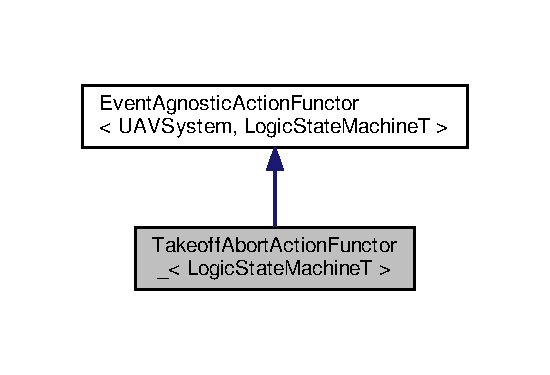
\includegraphics[width=264pt]{structTakeoffAbortActionFunctor____inherit__graph}
\end{center}
\end{figure}


Collaboration diagram for Takeoff\-Abort\-Action\-Functor\-\_\-$<$ Logic\-State\-Machine\-T $>$\-:\nopagebreak
\begin{figure}[H]
\begin{center}
\leavevmode
\includegraphics[width=264pt]{structTakeoffAbortActionFunctor____coll__graph}
\end{center}
\end{figure}
\subsection*{Public Member Functions}
\begin{DoxyCompactItemize}
\item 
void \hyperlink{structTakeoffAbortActionFunctor___a8366919888a54d029b3856c3a433843d}{run} (\hyperlink{classUAVSystem}{U\-A\-V\-System} \&robot\-\_\-system, Logic\-State\-Machine\-T \&)
\begin{DoxyCompactList}\small\item\em Override this run function for different sub classes. This function performs the logic checking for each state. \end{DoxyCompactList}\end{DoxyCompactItemize}


\subsection{Detailed Description}
\subsubsection*{template$<$class Logic\-State\-Machine\-T$>$struct Takeoff\-Abort\-Action\-Functor\-\_\-$<$ Logic\-State\-Machine\-T $>$}

action to perform when aborting takeoff 


\begin{DoxyTemplParams}{Template Parameters}
{\em Logic\-State\-Machine\-T} & Logic state machine used to process events \\
\hline
\end{DoxyTemplParams}


\subsection{Member Function Documentation}
\hypertarget{structTakeoffAbortActionFunctor___a8366919888a54d029b3856c3a433843d}{\index{Takeoff\-Abort\-Action\-Functor\-\_\-@{Takeoff\-Abort\-Action\-Functor\-\_\-}!run@{run}}
\index{run@{run}!TakeoffAbortActionFunctor_@{Takeoff\-Abort\-Action\-Functor\-\_\-}}
\subsubsection[{run}]{\setlength{\rightskip}{0pt plus 5cm}template$<$class Logic\-State\-Machine\-T $>$ void {\bf Takeoff\-Abort\-Action\-Functor\-\_\-}$<$ Logic\-State\-Machine\-T $>$\-::run (
\begin{DoxyParamCaption}
\item[{{\bf U\-A\-V\-System} \&}]{robot\-\_\-system, }
\item[{Logic\-State\-Machine\-T \&}]{logic\-\_\-state\-\_\-machine}
\end{DoxyParamCaption}
)\hspace{0.3cm}{\ttfamily [inline]}, {\ttfamily [virtual]}}}\label{structTakeoffAbortActionFunctor___a8366919888a54d029b3856c3a433843d}


Override this run function for different sub classes. This function performs the logic checking for each state. 


\begin{DoxyParams}{Parameters}
{\em robot\-\_\-system} & Provides sensor data and allows for controlling hardware \\
\hline
{\em logic\-\_\-state\-\_\-machine} & Backend of logic State Machine. can send events using this. \\
\hline
\end{DoxyParams}


Implements \hyperlink{structEventAgnosticActionFunctor_a53a48938d68370ff2ef262222565ffcf}{Event\-Agnostic\-Action\-Functor$<$ U\-A\-V\-System, Logic\-State\-Machine\-T $>$}.



The documentation for this struct was generated from the following file\-:\begin{DoxyCompactItemize}
\item 
include/aerial\-\_\-autonomy/actions\-\_\-guards/\hyperlink{takeoff__functors_8h}{takeoff\-\_\-functors.\-h}\end{DoxyCompactItemize}

\hypertarget{structTakeoffInternalActionFunctor__}{\section{Takeoff\-Internal\-Action\-Functor\-\_\-$<$ Logic\-State\-Machine\-T $>$ Struct Template Reference}
\label{structTakeoffInternalActionFunctor__}\index{Takeoff\-Internal\-Action\-Functor\-\_\-$<$ Logic\-State\-Machine\-T $>$@{Takeoff\-Internal\-Action\-Functor\-\_\-$<$ Logic\-State\-Machine\-T $>$}}
}


Check when takeoff is complete, and ensure enough battery voltage.  




{\ttfamily \#include $<$takeoff\-\_\-functors.\-h$>$}



Inheritance diagram for Takeoff\-Internal\-Action\-Functor\-\_\-$<$ Logic\-State\-Machine\-T $>$\-:\nopagebreak
\begin{figure}[H]
\begin{center}
\leavevmode
\includegraphics[width=264pt]{structTakeoffInternalActionFunctor____inherit__graph}
\end{center}
\end{figure}


Collaboration diagram for Takeoff\-Internal\-Action\-Functor\-\_\-$<$ Logic\-State\-Machine\-T $>$\-:\nopagebreak
\begin{figure}[H]
\begin{center}
\leavevmode
\includegraphics[width=264pt]{structTakeoffInternalActionFunctor____coll__graph}
\end{center}
\end{figure}
\subsection*{Public Member Functions}
\begin{DoxyCompactItemize}
\item 
void \hyperlink{structTakeoffInternalActionFunctor___a2118df6e326662cd0088344499e49696}{run} (\hyperlink{classUAVSystem}{U\-A\-V\-System} \&robot\-\_\-system, Logic\-State\-Machine\-T \&logic\-\_\-state\-\_\-machine)
\begin{DoxyCompactList}\small\item\em Function to check when takeoff is complete. If battery is low while takeoff, trigger Land event. \end{DoxyCompactList}\end{DoxyCompactItemize}


\subsection{Detailed Description}
\subsubsection*{template$<$class Logic\-State\-Machine\-T$>$struct Takeoff\-Internal\-Action\-Functor\-\_\-$<$ Logic\-State\-Machine\-T $>$}

Check when takeoff is complete, and ensure enough battery voltage. 


\begin{DoxyTemplParams}{Template Parameters}
{\em Logic\-State\-Machine\-T} & Logic state machine used to process events \\
\hline
\end{DoxyTemplParams}


\subsection{Member Function Documentation}
\hypertarget{structTakeoffInternalActionFunctor___a2118df6e326662cd0088344499e49696}{\index{Takeoff\-Internal\-Action\-Functor\-\_\-@{Takeoff\-Internal\-Action\-Functor\-\_\-}!run@{run}}
\index{run@{run}!TakeoffInternalActionFunctor_@{Takeoff\-Internal\-Action\-Functor\-\_\-}}
\subsubsection[{run}]{\setlength{\rightskip}{0pt plus 5cm}template$<$class Logic\-State\-Machine\-T $>$ void {\bf Takeoff\-Internal\-Action\-Functor\-\_\-}$<$ Logic\-State\-Machine\-T $>$\-::run (
\begin{DoxyParamCaption}
\item[{{\bf U\-A\-V\-System} \&}]{robot\-\_\-system, }
\item[{Logic\-State\-Machine\-T \&}]{logic\-\_\-state\-\_\-machine}
\end{DoxyParamCaption}
)\hspace{0.3cm}{\ttfamily [inline]}, {\ttfamily [virtual]}}}\label{structTakeoffInternalActionFunctor___a2118df6e326662cd0088344499e49696}


Function to check when takeoff is complete. If battery is low while takeoff, trigger Land event. 

\begin{DoxyRefDesc}{Todo}
\item[\hyperlink{todo__todo000010}{Todo}]add a parameter for height when to transition from takeoff to hovering\end{DoxyRefDesc}



\begin{DoxyParams}{Parameters}
{\em robot\-\_\-system} & robot system to get sensor data \\
\hline
{\em logic\-\_\-state\-\_\-machine} & logic state machine to trigger events \\
\hline
\end{DoxyParams}


Implements \hyperlink{structEventAgnosticActionFunctor_a53a48938d68370ff2ef262222565ffcf}{Event\-Agnostic\-Action\-Functor$<$ U\-A\-V\-System, Logic\-State\-Machine\-T $>$}.



The documentation for this struct was generated from the following file\-:\begin{DoxyCompactItemize}
\item 
include/aerial\-\_\-autonomy/actions\-\_\-guards/\hyperlink{takeoff__functors_8h}{takeoff\-\_\-functors.\-h}\end{DoxyCompactItemize}

\hypertarget{structTakeoffTransitionActionFunctor__}{\section{Takeoff\-Transition\-Action\-Functor\-\_\-$<$ Logic\-State\-Machine\-T $>$ Struct Template Reference}
\label{structTakeoffTransitionActionFunctor__}\index{Takeoff\-Transition\-Action\-Functor\-\_\-$<$ Logic\-State\-Machine\-T $>$@{Takeoff\-Transition\-Action\-Functor\-\_\-$<$ Logic\-State\-Machine\-T $>$}}
}


action to take when starting takeoff  




{\ttfamily \#include $<$takeoff\-\_\-functors.\-h$>$}



Inheritance diagram for Takeoff\-Transition\-Action\-Functor\-\_\-$<$ Logic\-State\-Machine\-T $>$\-:\nopagebreak
\begin{figure}[H]
\begin{center}
\leavevmode
\includegraphics[width=264pt]{structTakeoffTransitionActionFunctor____inherit__graph}
\end{center}
\end{figure}


Collaboration diagram for Takeoff\-Transition\-Action\-Functor\-\_\-$<$ Logic\-State\-Machine\-T $>$\-:\nopagebreak
\begin{figure}[H]
\begin{center}
\leavevmode
\includegraphics[width=264pt]{structTakeoffTransitionActionFunctor____coll__graph}
\end{center}
\end{figure}
\subsection*{Public Member Functions}
\begin{DoxyCompactItemize}
\item 
void \hyperlink{structTakeoffTransitionActionFunctor___aaf8ba8ac8cf0f07e2978da244b5efb2b}{run} (\hyperlink{classUAVSystem}{U\-A\-V\-System} \&robot\-\_\-system, Logic\-State\-Machine\-T \&)
\begin{DoxyCompactList}\small\item\em Override this run function for different sub classes. This function performs the logic checking for each state. \end{DoxyCompactList}\end{DoxyCompactItemize}


\subsection{Detailed Description}
\subsubsection*{template$<$class Logic\-State\-Machine\-T$>$struct Takeoff\-Transition\-Action\-Functor\-\_\-$<$ Logic\-State\-Machine\-T $>$}

action to take when starting takeoff 


\begin{DoxyTemplParams}{Template Parameters}
{\em Logic\-State\-Machine\-T} & Logic state machine used to process events \\
\hline
\end{DoxyTemplParams}


\subsection{Member Function Documentation}
\hypertarget{structTakeoffTransitionActionFunctor___aaf8ba8ac8cf0f07e2978da244b5efb2b}{\index{Takeoff\-Transition\-Action\-Functor\-\_\-@{Takeoff\-Transition\-Action\-Functor\-\_\-}!run@{run}}
\index{run@{run}!TakeoffTransitionActionFunctor_@{Takeoff\-Transition\-Action\-Functor\-\_\-}}
\subsubsection[{run}]{\setlength{\rightskip}{0pt plus 5cm}template$<$class Logic\-State\-Machine\-T $>$ void {\bf Takeoff\-Transition\-Action\-Functor\-\_\-}$<$ Logic\-State\-Machine\-T $>$\-::run (
\begin{DoxyParamCaption}
\item[{{\bf U\-A\-V\-System} \&}]{robot\-\_\-system, }
\item[{Logic\-State\-Machine\-T \&}]{logic\-\_\-state\-\_\-machine}
\end{DoxyParamCaption}
)\hspace{0.3cm}{\ttfamily [inline]}, {\ttfamily [virtual]}}}\label{structTakeoffTransitionActionFunctor___aaf8ba8ac8cf0f07e2978da244b5efb2b}


Override this run function for different sub classes. This function performs the logic checking for each state. 


\begin{DoxyParams}{Parameters}
{\em robot\-\_\-system} & Provides sensor data and allows for controlling hardware \\
\hline
{\em logic\-\_\-state\-\_\-machine} & Backend of logic State Machine. can send events using this. \\
\hline
\end{DoxyParams}


Implements \hyperlink{structEventAgnosticActionFunctor_a53a48938d68370ff2ef262222565ffcf}{Event\-Agnostic\-Action\-Functor$<$ U\-A\-V\-System, Logic\-State\-Machine\-T $>$}.



The documentation for this struct was generated from the following file\-:\begin{DoxyCompactItemize}
\item 
include/aerial\-\_\-autonomy/actions\-\_\-guards/\hyperlink{takeoff__functors_8h}{takeoff\-\_\-functors.\-h}\end{DoxyCompactItemize}

\hypertarget{structTakeoffTransitionGuardFunctor__}{\section{Takeoff\-Transition\-Guard\-Functor\-\_\-$<$ Logic\-State\-Machine\-T $>$ Struct Template Reference}
\label{structTakeoffTransitionGuardFunctor__}\index{Takeoff\-Transition\-Guard\-Functor\-\_\-$<$ Logic\-State\-Machine\-T $>$@{Takeoff\-Transition\-Guard\-Functor\-\_\-$<$ Logic\-State\-Machine\-T $>$}}
}


Guard to avoid accidental takeoff.  




{\ttfamily \#include $<$takeoff\-\_\-functors.\-h$>$}



Inheritance diagram for Takeoff\-Transition\-Guard\-Functor\-\_\-$<$ Logic\-State\-Machine\-T $>$\-:\nopagebreak
\begin{figure}[H]
\begin{center}
\leavevmode
\includegraphics[width=264pt]{structTakeoffTransitionGuardFunctor____inherit__graph}
\end{center}
\end{figure}


Collaboration diagram for Takeoff\-Transition\-Guard\-Functor\-\_\-$<$ Logic\-State\-Machine\-T $>$\-:\nopagebreak
\begin{figure}[H]
\begin{center}
\leavevmode
\includegraphics[width=264pt]{structTakeoffTransitionGuardFunctor____coll__graph}
\end{center}
\end{figure}
\subsection*{Public Member Functions}
\begin{DoxyCompactItemize}
\item 
bool \hyperlink{structTakeoffTransitionGuardFunctor___abef370db0002076671a6f9c2adb9bbaa}{guard} (\hyperlink{classUAVSystem}{U\-A\-V\-System} \&robot\-\_\-system, Logic\-State\-Machine\-T \&)
\begin{DoxyCompactList}\small\item\em Override this run function for different sub classes. This function performs the logic checking for each state. \end{DoxyCompactList}\end{DoxyCompactItemize}


\subsection{Detailed Description}
\subsubsection*{template$<$class Logic\-State\-Machine\-T$>$struct Takeoff\-Transition\-Guard\-Functor\-\_\-$<$ Logic\-State\-Machine\-T $>$}

Guard to avoid accidental takeoff. 


\begin{DoxyTemplParams}{Template Parameters}
{\em Logic\-State\-Machine\-T} & Logic state machine used to process events \\
\hline
\end{DoxyTemplParams}


\subsection{Member Function Documentation}
\hypertarget{structTakeoffTransitionGuardFunctor___abef370db0002076671a6f9c2adb9bbaa}{\index{Takeoff\-Transition\-Guard\-Functor\-\_\-@{Takeoff\-Transition\-Guard\-Functor\-\_\-}!guard@{guard}}
\index{guard@{guard}!TakeoffTransitionGuardFunctor_@{Takeoff\-Transition\-Guard\-Functor\-\_\-}}
\subsubsection[{guard}]{\setlength{\rightskip}{0pt plus 5cm}template$<$class Logic\-State\-Machine\-T $>$ bool {\bf Takeoff\-Transition\-Guard\-Functor\-\_\-}$<$ Logic\-State\-Machine\-T $>$\-::guard (
\begin{DoxyParamCaption}
\item[{{\bf U\-A\-V\-System} \&}]{robot\-\_\-system, }
\item[{Logic\-State\-Machine\-T \&}]{logic\-\_\-state\-\_\-machine}
\end{DoxyParamCaption}
)\hspace{0.3cm}{\ttfamily [inline]}, {\ttfamily [virtual]}}}\label{structTakeoffTransitionGuardFunctor___abef370db0002076671a6f9c2adb9bbaa}


Override this run function for different sub classes. This function performs the logic checking for each state. 


\begin{DoxyParams}{Parameters}
{\em robot\-\_\-system} & Provides sensor data and allows for controlling hardware \\
\hline
{\em logic\-\_\-state\-\_\-machine} & Backend of logic State Machine. can send events using this. \\
\hline
\end{DoxyParams}


Implements \hyperlink{structEventAgnosticGuardFunctor_ad97196f6a607d199d6dbd56156b8dd8c}{Event\-Agnostic\-Guard\-Functor$<$ U\-A\-V\-System, Logic\-State\-Machine\-T $>$}.



The documentation for this struct was generated from the following file\-:\begin{DoxyCompactItemize}
\item 
include/aerial\-\_\-autonomy/actions\-\_\-guards/\hyperlink{takeoff__functors_8h}{takeoff\-\_\-functors.\-h}\end{DoxyCompactItemize}

\hypertarget{classboost_1_1msm_1_1back_1_1thread__safe__state__machine}{\section{boost\-:\-:msm\-:\-:back\-:\-:thread\-\_\-safe\-\_\-state\-\_\-machine$<$ A0, A1, A2, A3, A4 $>$ Class Template Reference}
\label{classboost_1_1msm_1_1back_1_1thread__safe__state__machine}\index{boost\-::msm\-::back\-::thread\-\_\-safe\-\_\-state\-\_\-machine$<$ A0, A1, A2, A3, A4 $>$@{boost\-::msm\-::back\-::thread\-\_\-safe\-\_\-state\-\_\-machine$<$ A0, A1, A2, A3, A4 $>$}}
}


Thread safe state machine class that extends boost\-::msm\-::back\-::state\-\_\-machine class.  




{\ttfamily \#include $<$thread\-\_\-safe\-\_\-state\-\_\-machine.\-h$>$}



Inheritance diagram for boost\-:\-:msm\-:\-:back\-:\-:thread\-\_\-safe\-\_\-state\-\_\-machine$<$ A0, A1, A2, A3, A4 $>$\-:\nopagebreak
\begin{figure}[H]
\begin{center}
\leavevmode
\includegraphics[width=214pt]{classboost_1_1msm_1_1back_1_1thread__safe__state__machine__inherit__graph}
\end{center}
\end{figure}


Collaboration diagram for boost\-:\-:msm\-:\-:back\-:\-:thread\-\_\-safe\-\_\-state\-\_\-machine$<$ A0, A1, A2, A3, A4 $>$\-:\nopagebreak
\begin{figure}[H]
\begin{center}
\leavevmode
\includegraphics[width=214pt]{classboost_1_1msm_1_1back_1_1thread__safe__state__machine__coll__graph}
\end{center}
\end{figure}
\subsection*{Public Member Functions}
\begin{DoxyCompactItemize}
\item 
\hyperlink{classboost_1_1msm_1_1back_1_1thread__safe__state__machine_a5b5a31229aed12a1f7036b8b46de0884}{thread\-\_\-safe\-\_\-state\-\_\-machine} ()
\item 
{\footnotesize template$<$class Expr $>$ }\\\hyperlink{classboost_1_1msm_1_1back_1_1thread__safe__state__machine_ad8d554411680bddd9959406c42407c25}{thread\-\_\-safe\-\_\-state\-\_\-machine} (Expr const \&expr)
\item 
{\footnotesize template$<$class Event $>$ }\\execute\-\_\-return \hyperlink{classboost_1_1msm_1_1back_1_1thread__safe__state__machine_a9f38e619a54ce414c4ef737e8873928d}{process\-\_\-event} (Event const \&evt)
\begin{DoxyCompactList}\small\item\em The process event function that triggers transition actions in state machine The function is thread safe but does not execute the events in any particular order. \end{DoxyCompactList}\end{DoxyCompactItemize}
\subsection*{Friends}
\begin{DoxyCompactItemize}
\item 
{\footnotesize template$<$class , class , class , class , class $>$ }\\class \hyperlink{classboost_1_1msm_1_1back_1_1thread__safe__state__machine_a83a2deae1f2169f1234e430beb3b8a95}{boost\-::msm\-::back\-::state\-\_\-machine}
\item 
{\footnotesize template$<$class , class , class , class , class $>$ }\\class \hyperlink{classboost_1_1msm_1_1back_1_1thread__safe__state__machine_a3306dad625847fa2192b045a7789ca5f}{boost\-::msm\-::back\-::thread\-\_\-safe\-\_\-state\-\_\-machine}
\end{DoxyCompactItemize}


\subsection{Detailed Description}
\subsubsection*{template$<$class A0, class A1 = parameter\-::void\-\_\-, class A2 = parameter\-::void\-\_\-, class A3 = parameter\-::void\-\_\-, class A4 = parameter\-::void\-\_\-$>$class boost\-::msm\-::back\-::thread\-\_\-safe\-\_\-state\-\_\-machine$<$ A0, A1, A2, A3, A4 $>$}

Thread safe state machine class that extends boost\-::msm\-::back\-::state\-\_\-machine class. 

\subsection{Constructor \& Destructor Documentation}
\hypertarget{classboost_1_1msm_1_1back_1_1thread__safe__state__machine_a5b5a31229aed12a1f7036b8b46de0884}{\index{boost\-::msm\-::back\-::thread\-\_\-safe\-\_\-state\-\_\-machine@{boost\-::msm\-::back\-::thread\-\_\-safe\-\_\-state\-\_\-machine}!thread\-\_\-safe\-\_\-state\-\_\-machine@{thread\-\_\-safe\-\_\-state\-\_\-machine}}
\index{thread\-\_\-safe\-\_\-state\-\_\-machine@{thread\-\_\-safe\-\_\-state\-\_\-machine}!boost::msm::back::thread_safe_state_machine@{boost\-::msm\-::back\-::thread\-\_\-safe\-\_\-state\-\_\-machine}}
\subsubsection[{thread\-\_\-safe\-\_\-state\-\_\-machine}]{\setlength{\rightskip}{0pt plus 5cm}template$<$class A0 , class A1  = parameter\-::void\-\_\-, class A2  = parameter\-::void\-\_\-, class A3  = parameter\-::void\-\_\-, class A4  = parameter\-::void\-\_\-$>$ {\bf boost\-::msm\-::back\-::thread\-\_\-safe\-\_\-state\-\_\-machine}$<$ A0, A1, A2, A3, A4 $>$\-::{\bf thread\-\_\-safe\-\_\-state\-\_\-machine} (
\begin{DoxyParamCaption}
{}
\end{DoxyParamCaption}
)\hspace{0.3cm}{\ttfamily [inline]}}}\label{classboost_1_1msm_1_1back_1_1thread__safe__state__machine_a5b5a31229aed12a1f7036b8b46de0884}
\hypertarget{classboost_1_1msm_1_1back_1_1thread__safe__state__machine_ad8d554411680bddd9959406c42407c25}{\index{boost\-::msm\-::back\-::thread\-\_\-safe\-\_\-state\-\_\-machine@{boost\-::msm\-::back\-::thread\-\_\-safe\-\_\-state\-\_\-machine}!thread\-\_\-safe\-\_\-state\-\_\-machine@{thread\-\_\-safe\-\_\-state\-\_\-machine}}
\index{thread\-\_\-safe\-\_\-state\-\_\-machine@{thread\-\_\-safe\-\_\-state\-\_\-machine}!boost::msm::back::thread_safe_state_machine@{boost\-::msm\-::back\-::thread\-\_\-safe\-\_\-state\-\_\-machine}}
\subsubsection[{thread\-\_\-safe\-\_\-state\-\_\-machine}]{\setlength{\rightskip}{0pt plus 5cm}template$<$class A0 , class A1  = parameter\-::void\-\_\-, class A2  = parameter\-::void\-\_\-, class A3  = parameter\-::void\-\_\-, class A4  = parameter\-::void\-\_\-$>$ template$<$class Expr $>$ {\bf boost\-::msm\-::back\-::thread\-\_\-safe\-\_\-state\-\_\-machine}$<$ A0, A1, A2, A3, A4 $>$\-::{\bf thread\-\_\-safe\-\_\-state\-\_\-machine} (
\begin{DoxyParamCaption}
\item[{Expr const \&}]{expr}
\end{DoxyParamCaption}
)\hspace{0.3cm}{\ttfamily [inline]}}}\label{classboost_1_1msm_1_1back_1_1thread__safe__state__machine_ad8d554411680bddd9959406c42407c25}


\subsection{Member Function Documentation}
\hypertarget{classboost_1_1msm_1_1back_1_1thread__safe__state__machine_a9f38e619a54ce414c4ef737e8873928d}{\index{boost\-::msm\-::back\-::thread\-\_\-safe\-\_\-state\-\_\-machine@{boost\-::msm\-::back\-::thread\-\_\-safe\-\_\-state\-\_\-machine}!process\-\_\-event@{process\-\_\-event}}
\index{process\-\_\-event@{process\-\_\-event}!boost::msm::back::thread_safe_state_machine@{boost\-::msm\-::back\-::thread\-\_\-safe\-\_\-state\-\_\-machine}}
\subsubsection[{process\-\_\-event}]{\setlength{\rightskip}{0pt plus 5cm}template$<$class A0 , class A1  = parameter\-::void\-\_\-, class A2  = parameter\-::void\-\_\-, class A3  = parameter\-::void\-\_\-, class A4  = parameter\-::void\-\_\-$>$ template$<$class Event $>$ execute\-\_\-return {\bf boost\-::msm\-::back\-::thread\-\_\-safe\-\_\-state\-\_\-machine}$<$ A0, A1, A2, A3, A4 $>$\-::process\-\_\-event (
\begin{DoxyParamCaption}
\item[{Event const \&}]{evt}
\end{DoxyParamCaption}
)\hspace{0.3cm}{\ttfamily [inline]}}}\label{classboost_1_1msm_1_1back_1_1thread__safe__state__machine_a9f38e619a54ce414c4ef737e8873928d}


The process event function that triggers transition actions in state machine The function is thread safe but does not execute the events in any particular order. 


\begin{DoxyTemplParams}{Template Parameters}
{\em Event} & The event type that is received \\
\hline
\end{DoxyTemplParams}

\begin{DoxyParams}{Parameters}
{\em evt} & Instance of event type received by this function\\
\hline
\end{DoxyParams}
\begin{DoxyReturn}{Returns}
Enum specifying whether the event is handled, deferred etc. 
\end{DoxyReturn}


\subsection{Friends And Related Function Documentation}
\hypertarget{classboost_1_1msm_1_1back_1_1thread__safe__state__machine_a83a2deae1f2169f1234e430beb3b8a95}{\index{boost\-::msm\-::back\-::thread\-\_\-safe\-\_\-state\-\_\-machine@{boost\-::msm\-::back\-::thread\-\_\-safe\-\_\-state\-\_\-machine}!boost\-::msm\-::back\-::state\-\_\-machine@{boost\-::msm\-::back\-::state\-\_\-machine}}
\index{boost\-::msm\-::back\-::state\-\_\-machine@{boost\-::msm\-::back\-::state\-\_\-machine}!boost::msm::back::thread_safe_state_machine@{boost\-::msm\-::back\-::thread\-\_\-safe\-\_\-state\-\_\-machine}}
\subsubsection[{boost\-::msm\-::back\-::state\-\_\-machine}]{\setlength{\rightskip}{0pt plus 5cm}template$<$class A0 , class A1  = parameter\-::void\-\_\-, class A2  = parameter\-::void\-\_\-, class A3  = parameter\-::void\-\_\-, class A4  = parameter\-::void\-\_\-$>$ template$<$class , class , class , class , class $>$ friend class boost\-::msm\-::back\-::state\-\_\-machine\hspace{0.3cm}{\ttfamily [friend]}}}\label{classboost_1_1msm_1_1back_1_1thread__safe__state__machine_a83a2deae1f2169f1234e430beb3b8a95}
\hypertarget{classboost_1_1msm_1_1back_1_1thread__safe__state__machine_a3306dad625847fa2192b045a7789ca5f}{\index{boost\-::msm\-::back\-::thread\-\_\-safe\-\_\-state\-\_\-machine@{boost\-::msm\-::back\-::thread\-\_\-safe\-\_\-state\-\_\-machine}!boost\-::msm\-::back\-::thread\-\_\-safe\-\_\-state\-\_\-machine@{boost\-::msm\-::back\-::thread\-\_\-safe\-\_\-state\-\_\-machine}}
\index{boost\-::msm\-::back\-::thread\-\_\-safe\-\_\-state\-\_\-machine@{boost\-::msm\-::back\-::thread\-\_\-safe\-\_\-state\-\_\-machine}!boost::msm::back::thread_safe_state_machine@{boost\-::msm\-::back\-::thread\-\_\-safe\-\_\-state\-\_\-machine}}
\subsubsection[{boost\-::msm\-::back\-::thread\-\_\-safe\-\_\-state\-\_\-machine}]{\setlength{\rightskip}{0pt plus 5cm}template$<$class A0 , class A1  = parameter\-::void\-\_\-, class A2  = parameter\-::void\-\_\-, class A3  = parameter\-::void\-\_\-, class A4  = parameter\-::void\-\_\-$>$ template$<$class , class , class , class , class $>$ friend class {\bf boost\-::msm\-::back\-::thread\-\_\-safe\-\_\-state\-\_\-machine}\hspace{0.3cm}{\ttfamily [friend]}}}\label{classboost_1_1msm_1_1back_1_1thread__safe__state__machine_a3306dad625847fa2192b045a7789ca5f}


The documentation for this class was generated from the following file\-:\begin{DoxyCompactItemize}
\item 
include/aerial\-\_\-autonomy/common/\hyperlink{thread__safe__state__machine_8h}{thread\-\_\-safe\-\_\-state\-\_\-machine.\-h}\end{DoxyCompactItemize}

\hypertarget{structLogicStateMachineFrontEnd_1_1transition__table}{\section{Logic\-State\-Machine\-Front\-End\-:\-:transition\-\_\-table Struct Reference}
\label{structLogicStateMachineFrontEnd_1_1transition__table}\index{Logic\-State\-Machine\-Front\-End\-::transition\-\_\-table@{Logic\-State\-Machine\-Front\-End\-::transition\-\_\-table}}
}


Transition table for State Machine.  




{\ttfamily \#include $<$basic\-\_\-state\-\_\-machine.\-h$>$}



Inheritance diagram for Logic\-State\-Machine\-Front\-End\-:\-:transition\-\_\-table\-:\nopagebreak
\begin{figure}[H]
\begin{center}
\leavevmode
\includegraphics[width=350pt]{structLogicStateMachineFrontEnd_1_1transition__table__inherit__graph}
\end{center}
\end{figure}


Collaboration diagram for Logic\-State\-Machine\-Front\-End\-:\-:transition\-\_\-table\-:\nopagebreak
\begin{figure}[H]
\begin{center}
\leavevmode
\includegraphics[width=350pt]{structLogicStateMachineFrontEnd_1_1transition__table__coll__graph}
\end{center}
\end{figure}


\subsection{Detailed Description}
Transition table for State Machine. 

The documentation for this struct was generated from the following file\-:\begin{DoxyCompactItemize}
\item 
include/aerial\-\_\-autonomy/state\-\_\-machines/\hyperlink{basic__state__machine_8h}{basic\-\_\-state\-\_\-machine.\-h}\end{DoxyCompactItemize}

\hypertarget{classTypeMap}{\section{Type\-Map$<$ Generic\-Object\-T $>$ Class Template Reference}
\label{classTypeMap}\index{Type\-Map$<$ Generic\-Object\-T $>$@{Type\-Map$<$ Generic\-Object\-T $>$}}
}


Store objects with a common base class.  




{\ttfamily \#include $<$type\-\_\-map.\-h$>$}

\subsection*{Public Member Functions}
\begin{DoxyCompactItemize}
\item 
{\footnotesize template$<$class Object\-T $>$ }\\void \hyperlink{classTypeMap_a738b13adaac930d128c1a81b08628b9e}{set\-Object} (Object\-T \&object)
\begin{DoxyCompactList}\small\item\em Store the object with base class as Generic\-Object\-T. \end{DoxyCompactList}\item 
{\footnotesize template$<$class Object\-T $>$ }\\Object\-T $\ast$ \hyperlink{classTypeMap_af45351278345a92d2d2fb13a977858aa}{get\-Object} ()
\begin{DoxyCompactList}\small\item\em return the object stored \end{DoxyCompactList}\end{DoxyCompactItemize}


\subsection{Detailed Description}
\subsubsection*{template$<$class Generic\-Object\-T$>$class Type\-Map$<$ Generic\-Object\-T $>$}

Store objects with a common base class. 


\begin{DoxyTemplParams}{Template Parameters}
{\em Generic\-Object\-T} & Common base class for objects stored \\
\hline
\end{DoxyTemplParams}


\subsection{Member Function Documentation}
\hypertarget{classTypeMap_af45351278345a92d2d2fb13a977858aa}{\index{Type\-Map@{Type\-Map}!get\-Object@{get\-Object}}
\index{get\-Object@{get\-Object}!TypeMap@{Type\-Map}}
\subsubsection[{get\-Object}]{\setlength{\rightskip}{0pt plus 5cm}template$<$class Generic\-Object\-T$>$ template$<$class Object\-T $>$ Object\-T$\ast$ {\bf Type\-Map}$<$ Generic\-Object\-T $>$\-::get\-Object (
\begin{DoxyParamCaption}
{}
\end{DoxyParamCaption}
)\hspace{0.3cm}{\ttfamily [inline]}}}\label{classTypeMap_af45351278345a92d2d2fb13a977858aa}


return the object stored 


\begin{DoxyTemplParams}{Template Parameters}
{\em Object\-T} & type of object to be retrieved.\\
\hline
\end{DoxyTemplParams}
\begin{DoxyReturn}{Returns}
pointer to the instance of the object. 
\end{DoxyReturn}
\hypertarget{classTypeMap_a738b13adaac930d128c1a81b08628b9e}{\index{Type\-Map@{Type\-Map}!set\-Object@{set\-Object}}
\index{set\-Object@{set\-Object}!TypeMap@{Type\-Map}}
\subsubsection[{set\-Object}]{\setlength{\rightskip}{0pt plus 5cm}template$<$class Generic\-Object\-T$>$ template$<$class Object\-T $>$ void {\bf Type\-Map}$<$ Generic\-Object\-T $>$\-::set\-Object (
\begin{DoxyParamCaption}
\item[{Object\-T \&}]{object}
\end{DoxyParamCaption}
)\hspace{0.3cm}{\ttfamily [inline]}}}\label{classTypeMap_a738b13adaac930d128c1a81b08628b9e}


Store the object with base class as Generic\-Object\-T. 


\begin{DoxyTemplParams}{Template Parameters}
{\em Object\-T} & The type of object being stored. Object\-T should be base class of Generic\-Object\-T \\
\hline
\end{DoxyTemplParams}

\begin{DoxyParams}{Parameters}
{\em object} & The address of an instance of Object\-T being stored \\
\hline
\end{DoxyParams}


The documentation for this class was generated from the following file\-:\begin{DoxyCompactItemize}
\item 
include/aerial\-\_\-autonomy/common/\hyperlink{type__map_8h}{type\-\_\-map.\-h}\end{DoxyCompactItemize}

\hypertarget{classUAVSystem}{\section{U\-A\-V\-System Class Reference}
\label{classUAVSystem}\index{U\-A\-V\-System@{U\-A\-V\-System}}
}


Owns, initializes, and facilitates communication between different hardware/software components. Provides builtin position, velocity, and rpy controllers for controlling U\-A\-V.  




{\ttfamily \#include $<$uav\-\_\-system.\-h$>$}

\subsection*{Public Member Functions}
\begin{DoxyCompactItemize}
\item 
\hyperlink{classUAVSystem_a99ac3986113a03546b8dc4bcc73d65b0}{U\-A\-V\-System} (parsernode\-::\-Parser \&drone\-\_\-hardware)
\begin{DoxyCompactList}\small\item\em Constructor with default configuration. \end{DoxyCompactList}\item 
\hyperlink{classUAVSystem_a9218f794905e832cc356b5e4b659e1da}{U\-A\-V\-System} (parsernode\-::\-Parser \&drone\-\_\-hardware, U\-A\-V\-System\-Config config)
\begin{DoxyCompactList}\small\item\em Constructor. \end{DoxyCompactList}\item 
parsernode\-::common\-::quaddata \hyperlink{classUAVSystem_a8a1cbcd8770841ee2a30365f4a75bf34}{get\-U\-A\-V\-Data} ()
\begin{DoxyCompactList}\small\item\em Get sensor data from U\-A\-V. \end{DoxyCompactList}\item 
void \hyperlink{classUAVSystem_a7f010477b67bfeb5d6d32c0f10630b8e}{take\-Off} ()
\begin{DoxyCompactList}\small\item\em Public A\-P\-I call to takeoff. \end{DoxyCompactList}\item 
void \hyperlink{classUAVSystem_ae1bac31ca121a54cb1e3ed7fac322993}{land} ()
\begin{DoxyCompactList}\small\item\em Public A\-P\-I call to land. \end{DoxyCompactList}\item 
{\footnotesize template$<$class Controller\-Hardware\-Connector\-T , class Goal\-T $>$ }\\void \hyperlink{classUAVSystem_a6aae5b94424be17ed6bafeaa4f64f416}{set\-Goal} (Goal\-T goal)
\begin{DoxyCompactList}\small\item\em sets goal to the connector and swaps the active connector with the specified connector type. \end{DoxyCompactList}\item 
{\footnotesize template$<$class Controller\-Hardware\-Connector\-T , class Goal\-T $>$ }\\Goal\-T \hyperlink{classUAVSystem_a5381ca45049c8c92e872a80a2974339b}{get\-Goal} ()
\begin{DoxyCompactList}\small\item\em Get the goal from connector. \end{DoxyCompactList}\item 
void \hyperlink{classUAVSystem_a90634eb2ac4c515c9065ce85cc21dc19}{abort\-Controller} (\hyperlink{base__controller__hardware__connector_8h_ae4dfd42394001deb6e8a0e60c81d6f7a}{Hardware\-Type} hardware\-\_\-type)
\begin{DoxyCompactList}\small\item\em Remove active controller for given hardware type. \end{DoxyCompactList}\item 
void \hyperlink{classUAVSystem_ad3d60a491f325261a1acebdadd7478a6}{run\-Active\-Controller} (\hyperlink{base__controller__hardware__connector_8h_ae4dfd42394001deb6e8a0e60c81d6f7a}{Hardware\-Type} hardware\-\_\-type)
\begin{DoxyCompactList}\small\item\em Run active controller stored for a given hardware type. \end{DoxyCompactList}\item 
std\-::string \hyperlink{classUAVSystem_ab0840278177ee64082ee05937d028421}{get\-System\-Status} ()
\item 
U\-A\-V\-System\-Config \hyperlink{classUAVSystem_a89d67e42aec09dd65a23f39462a8202e}{get\-Configuration} ()
\begin{DoxyCompactList}\small\item\em Get system configuration. \end{DoxyCompactList}\end{DoxyCompactItemize}


\subsection{Detailed Description}
Owns, initializes, and facilitates communication between different hardware/software components. Provides builtin position, velocity, and rpy controllers for controlling U\-A\-V. 

\subsection{Constructor \& Destructor Documentation}
\hypertarget{classUAVSystem_a99ac3986113a03546b8dc4bcc73d65b0}{\index{U\-A\-V\-System@{U\-A\-V\-System}!U\-A\-V\-System@{U\-A\-V\-System}}
\index{U\-A\-V\-System@{U\-A\-V\-System}!UAVSystem@{U\-A\-V\-System}}
\subsubsection[{U\-A\-V\-System}]{\setlength{\rightskip}{0pt plus 5cm}U\-A\-V\-System\-::\-U\-A\-V\-System (
\begin{DoxyParamCaption}
\item[{parsernode\-::\-Parser \&}]{drone\-\_\-hardware}
\end{DoxyParamCaption}
)\hspace{0.3cm}{\ttfamily [inline]}}}\label{classUAVSystem_a99ac3986113a03546b8dc4bcc73d65b0}


Constructor with default configuration. 

\hypertarget{classUAVSystem_a9218f794905e832cc356b5e4b659e1da}{\index{U\-A\-V\-System@{U\-A\-V\-System}!U\-A\-V\-System@{U\-A\-V\-System}}
\index{U\-A\-V\-System@{U\-A\-V\-System}!UAVSystem@{U\-A\-V\-System}}
\subsubsection[{U\-A\-V\-System}]{\setlength{\rightskip}{0pt plus 5cm}U\-A\-V\-System\-::\-U\-A\-V\-System (
\begin{DoxyParamCaption}
\item[{parsernode\-::\-Parser \&}]{drone\-\_\-hardware, }
\item[{U\-A\-V\-System\-Config}]{config}
\end{DoxyParamCaption}
)\hspace{0.3cm}{\ttfamily [inline]}}}\label{classUAVSystem_a9218f794905e832cc356b5e4b659e1da}


Constructor. 

\hyperlink{classUAVSystem}{U\-A\-V\-System} requires a drone hardware. It instantiates the connectors, controllers


\begin{DoxyParams}{Parameters}
{\em drone\-\_\-hardware} & input hardware to send commands back \\
\hline
\end{DoxyParams}
\begin{DoxyRefDesc}{Todo}
\item[\hyperlink{todo__todo000012}{Todo}]make enum class iterable to do this automatically \end{DoxyRefDesc}


\subsection{Member Function Documentation}
\hypertarget{classUAVSystem_a90634eb2ac4c515c9065ce85cc21dc19}{\index{U\-A\-V\-System@{U\-A\-V\-System}!abort\-Controller@{abort\-Controller}}
\index{abort\-Controller@{abort\-Controller}!UAVSystem@{U\-A\-V\-System}}
\subsubsection[{abort\-Controller}]{\setlength{\rightskip}{0pt plus 5cm}void U\-A\-V\-System\-::abort\-Controller (
\begin{DoxyParamCaption}
\item[{{\bf Hardware\-Type}}]{hardware\-\_\-type}
\end{DoxyParamCaption}
)\hspace{0.3cm}{\ttfamily [inline]}}}\label{classUAVSystem_a90634eb2ac4c515c9065ce85cc21dc19}


Remove active controller for given hardware type. 


\begin{DoxyParams}{Parameters}
{\em hardware\-\_\-type} & Type of hardware for which active controller is switched off \\
\hline
\end{DoxyParams}
\hypertarget{classUAVSystem_a89d67e42aec09dd65a23f39462a8202e}{\index{U\-A\-V\-System@{U\-A\-V\-System}!get\-Configuration@{get\-Configuration}}
\index{get\-Configuration@{get\-Configuration}!UAVSystem@{U\-A\-V\-System}}
\subsubsection[{get\-Configuration}]{\setlength{\rightskip}{0pt plus 5cm}U\-A\-V\-System\-Config U\-A\-V\-System\-::get\-Configuration (
\begin{DoxyParamCaption}
{}
\end{DoxyParamCaption}
)\hspace{0.3cm}{\ttfamily [inline]}}}\label{classUAVSystem_a89d67e42aec09dd65a23f39462a8202e}


Get system configuration. 

\begin{DoxyReturn}{Returns}
Configuration 
\end{DoxyReturn}
\hypertarget{classUAVSystem_a5381ca45049c8c92e872a80a2974339b}{\index{U\-A\-V\-System@{U\-A\-V\-System}!get\-Goal@{get\-Goal}}
\index{get\-Goal@{get\-Goal}!UAVSystem@{U\-A\-V\-System}}
\subsubsection[{get\-Goal}]{\setlength{\rightskip}{0pt plus 5cm}template$<$class Controller\-Hardware\-Connector\-T , class Goal\-T $>$ Goal\-T U\-A\-V\-System\-::get\-Goal (
\begin{DoxyParamCaption}
{}
\end{DoxyParamCaption}
)\hspace{0.3cm}{\ttfamily [inline]}}}\label{classUAVSystem_a5381ca45049c8c92e872a80a2974339b}


Get the goal from connector. 


\begin{DoxyTemplParams}{Template Parameters}
{\em Controller\-Hardware\-Connector\-T} & Type of connector to use \\
\hline
{\em Goal\-T} & Type of Goal to get\\
\hline
\end{DoxyTemplParams}
\begin{DoxyReturn}{Returns}
goal of Goal\-T type 
\end{DoxyReturn}
\hypertarget{classUAVSystem_ab0840278177ee64082ee05937d028421}{\index{U\-A\-V\-System@{U\-A\-V\-System}!get\-System\-Status@{get\-System\-Status}}
\index{get\-System\-Status@{get\-System\-Status}!UAVSystem@{U\-A\-V\-System}}
\subsubsection[{get\-System\-Status}]{\setlength{\rightskip}{0pt plus 5cm}std\-::string U\-A\-V\-System\-::get\-System\-Status (
\begin{DoxyParamCaption}
{}
\end{DoxyParamCaption}
)\hspace{0.3cm}{\ttfamily [inline]}}}\label{classUAVSystem_ab0840278177ee64082ee05937d028421}
\hypertarget{classUAVSystem_a8a1cbcd8770841ee2a30365f4a75bf34}{\index{U\-A\-V\-System@{U\-A\-V\-System}!get\-U\-A\-V\-Data@{get\-U\-A\-V\-Data}}
\index{get\-U\-A\-V\-Data@{get\-U\-A\-V\-Data}!UAVSystem@{U\-A\-V\-System}}
\subsubsection[{get\-U\-A\-V\-Data}]{\setlength{\rightskip}{0pt plus 5cm}parsernode\-::common\-::quaddata U\-A\-V\-System\-::get\-U\-A\-V\-Data (
\begin{DoxyParamCaption}
{}
\end{DoxyParamCaption}
)\hspace{0.3cm}{\ttfamily [inline]}}}\label{classUAVSystem_a8a1cbcd8770841ee2a30365f4a75bf34}


Get sensor data from U\-A\-V. 

\begin{DoxyReturn}{Returns}
Accumulated sensor data from U\-A\-V 
\end{DoxyReturn}
\hypertarget{classUAVSystem_ae1bac31ca121a54cb1e3ed7fac322993}{\index{U\-A\-V\-System@{U\-A\-V\-System}!land@{land}}
\index{land@{land}!UAVSystem@{U\-A\-V\-System}}
\subsubsection[{land}]{\setlength{\rightskip}{0pt plus 5cm}void U\-A\-V\-System\-::land (
\begin{DoxyParamCaption}
{}
\end{DoxyParamCaption}
)\hspace{0.3cm}{\ttfamily [inline]}}}\label{classUAVSystem_ae1bac31ca121a54cb1e3ed7fac322993}


Public A\-P\-I call to land. 

\hypertarget{classUAVSystem_ad3d60a491f325261a1acebdadd7478a6}{\index{U\-A\-V\-System@{U\-A\-V\-System}!run\-Active\-Controller@{run\-Active\-Controller}}
\index{run\-Active\-Controller@{run\-Active\-Controller}!UAVSystem@{U\-A\-V\-System}}
\subsubsection[{run\-Active\-Controller}]{\setlength{\rightskip}{0pt plus 5cm}void U\-A\-V\-System\-::run\-Active\-Controller (
\begin{DoxyParamCaption}
\item[{{\bf Hardware\-Type}}]{hardware\-\_\-type}
\end{DoxyParamCaption}
)\hspace{0.3cm}{\ttfamily [inline]}}}\label{classUAVSystem_ad3d60a491f325261a1acebdadd7478a6}


Run active controller stored for a given hardware type. 


\begin{DoxyParams}{Parameters}
{\em hardware\-\_\-type} & Type of hardware for which active controller is run \\
\hline
\end{DoxyParams}
\hypertarget{classUAVSystem_a6aae5b94424be17ed6bafeaa4f64f416}{\index{U\-A\-V\-System@{U\-A\-V\-System}!set\-Goal@{set\-Goal}}
\index{set\-Goal@{set\-Goal}!UAVSystem@{U\-A\-V\-System}}
\subsubsection[{set\-Goal}]{\setlength{\rightskip}{0pt plus 5cm}template$<$class Controller\-Hardware\-Connector\-T , class Goal\-T $>$ void U\-A\-V\-System\-::set\-Goal (
\begin{DoxyParamCaption}
\item[{Goal\-T}]{goal}
\end{DoxyParamCaption}
)\hspace{0.3cm}{\ttfamily [inline]}}}\label{classUAVSystem_a6aae5b94424be17ed6bafeaa4f64f416}


sets goal to the connector and swaps the active connector with the specified connector type. 


\begin{DoxyTemplParams}{Template Parameters}
{\em Controller\-Hardware\-Connector\-T} & type of connector to use \\
\hline
{\em Goal\-T} & Type of Goal to set to connector \\
\hline
\end{DoxyTemplParams}

\begin{DoxyParams}{Parameters}
{\em goal} & Goal to set to connector \\
\hline
\end{DoxyParams}
\hypertarget{classUAVSystem_a7f010477b67bfeb5d6d32c0f10630b8e}{\index{U\-A\-V\-System@{U\-A\-V\-System}!take\-Off@{take\-Off}}
\index{take\-Off@{take\-Off}!UAVSystem@{U\-A\-V\-System}}
\subsubsection[{take\-Off}]{\setlength{\rightskip}{0pt plus 5cm}void U\-A\-V\-System\-::take\-Off (
\begin{DoxyParamCaption}
{}
\end{DoxyParamCaption}
)\hspace{0.3cm}{\ttfamily [inline]}}}\label{classUAVSystem_a7f010477b67bfeb5d6d32c0f10630b8e}


Public A\-P\-I call to takeoff. 



The documentation for this class was generated from the following file\-:\begin{DoxyCompactItemize}
\item 
include/aerial\-\_\-autonomy/robot\-\_\-systems/\hyperlink{uav__system_8h}{uav\-\_\-system.\-h}\end{DoxyCompactItemize}

\hypertarget{structVelocity}{\section{Velocity Struct Reference}
\label{structVelocity}\index{Velocity@{Velocity}}
}


Store velocity vector.  




{\ttfamily \#include $<$velocity.\-h$>$}



Inheritance diagram for Velocity\-:\nopagebreak
\begin{figure}[H]
\begin{center}
\leavevmode
\includegraphics[width=150pt]{structVelocity__inherit__graph}
\end{center}
\end{figure}
\subsection*{Public Member Functions}
\begin{DoxyCompactItemize}
\item 
\hyperlink{structVelocity_a852088c8d4dbb7e1beb0d793a57e9d11}{Velocity} ()
\begin{DoxyCompactList}\small\item\em Constructor with implicit instantiation of velocity vector to zero. \end{DoxyCompactList}\item 
\hyperlink{structVelocity_adb5f7fd7a3e1811b44c9b4020c31987c}{Velocity} (double \hyperlink{structVelocity_a99a9f9580c8a025a2c7a18890993b56a}{x}, double \hyperlink{structVelocity_ae1282d20e14cc4be4aac24ab4e1e3e5c}{y}, double \hyperlink{structVelocity_aaebcd198674f7adcb61f9bb981dab465}{z})
\begin{DoxyCompactList}\small\item\em Constructor with explicit instantiation. \end{DoxyCompactList}\item 
bool \hyperlink{structVelocity_a4d148dc8c7581af4a1a16116ec3d403a}{operator==} (const \hyperlink{structVelocity}{Velocity} \&v) const 
\begin{DoxyCompactList}\small\item\em Check if two velocity vectors are the same. \end{DoxyCompactList}\item 
bool \hyperlink{structVelocity_a8aaa79fd50b42d41e06033be8baf4c80}{operator!=} (const \hyperlink{structVelocity}{Velocity} \&v) const 
\begin{DoxyCompactList}\small\item\em Check if two vectors are not equal. \end{DoxyCompactList}\end{DoxyCompactItemize}
\subsection*{Public Attributes}
\begin{DoxyCompactItemize}
\item 
double \hyperlink{structVelocity_a99a9f9580c8a025a2c7a18890993b56a}{x}
\begin{DoxyCompactList}\small\item\em x component in m/s \end{DoxyCompactList}\item 
double \hyperlink{structVelocity_ae1282d20e14cc4be4aac24ab4e1e3e5c}{y}
\begin{DoxyCompactList}\small\item\em y component in m/s \end{DoxyCompactList}\item 
double \hyperlink{structVelocity_aaebcd198674f7adcb61f9bb981dab465}{z}
\begin{DoxyCompactList}\small\item\em z component in m/s \end{DoxyCompactList}\end{DoxyCompactItemize}


\subsection{Detailed Description}
Store velocity vector. 

\subsection{Constructor \& Destructor Documentation}
\hypertarget{structVelocity_a852088c8d4dbb7e1beb0d793a57e9d11}{\index{Velocity@{Velocity}!Velocity@{Velocity}}
\index{Velocity@{Velocity}!Velocity@{Velocity}}
\subsubsection[{Velocity}]{\setlength{\rightskip}{0pt plus 5cm}Velocity\-::\-Velocity (
\begin{DoxyParamCaption}
{}
\end{DoxyParamCaption}
)\hspace{0.3cm}{\ttfamily [inline]}}}\label{structVelocity_a852088c8d4dbb7e1beb0d793a57e9d11}


Constructor with implicit instantiation of velocity vector to zero. 

\hypertarget{structVelocity_adb5f7fd7a3e1811b44c9b4020c31987c}{\index{Velocity@{Velocity}!Velocity@{Velocity}}
\index{Velocity@{Velocity}!Velocity@{Velocity}}
\subsubsection[{Velocity}]{\setlength{\rightskip}{0pt plus 5cm}Velocity\-::\-Velocity (
\begin{DoxyParamCaption}
\item[{double}]{x, }
\item[{double}]{y, }
\item[{double}]{z}
\end{DoxyParamCaption}
)\hspace{0.3cm}{\ttfamily [inline]}}}\label{structVelocity_adb5f7fd7a3e1811b44c9b4020c31987c}


Constructor with explicit instantiation. 


\begin{DoxyParams}{Parameters}
{\em x} & x component (m/s) \\
\hline
{\em y} & y component (m/s) \\
\hline
{\em z} & z component (m/s) \\
\hline
\end{DoxyParams}


\subsection{Member Function Documentation}
\hypertarget{structVelocity_a8aaa79fd50b42d41e06033be8baf4c80}{\index{Velocity@{Velocity}!operator!=@{operator!=}}
\index{operator!=@{operator!=}!Velocity@{Velocity}}
\subsubsection[{operator!=}]{\setlength{\rightskip}{0pt plus 5cm}bool Velocity\-::operator!= (
\begin{DoxyParamCaption}
\item[{const {\bf Velocity} \&}]{v}
\end{DoxyParamCaption}
) const\hspace{0.3cm}{\ttfamily [inline]}}}\label{structVelocity_a8aaa79fd50b42d41e06033be8baf4c80}


Check if two vectors are not equal. 


\begin{DoxyParams}{Parameters}
{\em v} & The vector agains which the current vector is compared.\\
\hline
\end{DoxyParams}
\begin{DoxyReturn}{Returns}
True if two vectors are not equal 
\end{DoxyReturn}
\hypertarget{structVelocity_a4d148dc8c7581af4a1a16116ec3d403a}{\index{Velocity@{Velocity}!operator==@{operator==}}
\index{operator==@{operator==}!Velocity@{Velocity}}
\subsubsection[{operator==}]{\setlength{\rightskip}{0pt plus 5cm}bool Velocity\-::operator== (
\begin{DoxyParamCaption}
\item[{const {\bf Velocity} \&}]{v}
\end{DoxyParamCaption}
) const\hspace{0.3cm}{\ttfamily [inline]}}}\label{structVelocity_a4d148dc8c7581af4a1a16116ec3d403a}


Check if two velocity vectors are the same. 


\begin{DoxyParams}{Parameters}
{\em v} & The vector agains which the current vector is compared.\\
\hline
\end{DoxyParams}
\begin{DoxyReturn}{Returns}
True if vectors are equal 
\end{DoxyReturn}


\subsection{Member Data Documentation}
\hypertarget{structVelocity_a99a9f9580c8a025a2c7a18890993b56a}{\index{Velocity@{Velocity}!x@{x}}
\index{x@{x}!Velocity@{Velocity}}
\subsubsection[{x}]{\setlength{\rightskip}{0pt plus 5cm}double Velocity\-::x}}\label{structVelocity_a99a9f9580c8a025a2c7a18890993b56a}


x component in m/s 

\hypertarget{structVelocity_ae1282d20e14cc4be4aac24ab4e1e3e5c}{\index{Velocity@{Velocity}!y@{y}}
\index{y@{y}!Velocity@{Velocity}}
\subsubsection[{y}]{\setlength{\rightskip}{0pt plus 5cm}double Velocity\-::y}}\label{structVelocity_ae1282d20e14cc4be4aac24ab4e1e3e5c}


y component in m/s 

\hypertarget{structVelocity_aaebcd198674f7adcb61f9bb981dab465}{\index{Velocity@{Velocity}!z@{z}}
\index{z@{z}!Velocity@{Velocity}}
\subsubsection[{z}]{\setlength{\rightskip}{0pt plus 5cm}double Velocity\-::z}}\label{structVelocity_aaebcd198674f7adcb61f9bb981dab465}


z component in m/s 



The documentation for this struct was generated from the following file\-:\begin{DoxyCompactItemize}
\item 
include/aerial\-\_\-autonomy/types/\hyperlink{velocity_8h}{velocity.\-h}\end{DoxyCompactItemize}

\hypertarget{structVelocityYaw}{\section{Velocity\-Yaw Struct Reference}
\label{structVelocityYaw}\index{Velocity\-Yaw@{Velocity\-Yaw}}
}


Store velocity and yaw Used as goal for builtin velocity and yaw controller for U\-A\-V system.  




{\ttfamily \#include $<$velocity\-\_\-yaw.\-h$>$}



Inheritance diagram for Velocity\-Yaw\-:\nopagebreak
\begin{figure}[H]
\begin{center}
\leavevmode
\includegraphics[width=150pt]{structVelocityYaw__inherit__graph}
\end{center}
\end{figure}


Collaboration diagram for Velocity\-Yaw\-:\nopagebreak
\begin{figure}[H]
\begin{center}
\leavevmode
\includegraphics[width=150pt]{structVelocityYaw__coll__graph}
\end{center}
\end{figure}
\subsection*{Public Member Functions}
\begin{DoxyCompactItemize}
\item 
\hyperlink{structVelocityYaw_a1aa3de4b3e3d7510c233ebd54b2fe79d}{Velocity\-Yaw} ()
\begin{DoxyCompactList}\small\item\em Implicit constructor Instantiates velocity and yaw to zero. \end{DoxyCompactList}\item 
\hyperlink{structVelocityYaw_a21a3493e39f5256972abe5f97315c80b}{Velocity\-Yaw} (\hyperlink{structVelocity}{Velocity} v, double \hyperlink{structVelocityYaw_a5bef45a2807a9814495080d2e5603ce4}{yaw})
\begin{DoxyCompactList}\small\item\em Explicit constructor. \end{DoxyCompactList}\item 
\hyperlink{structVelocityYaw_ab4ebb3f3782c9541dafb73c4e3e82196}{Velocity\-Yaw} (double \hyperlink{structVelocity_a99a9f9580c8a025a2c7a18890993b56a}{x}, double \hyperlink{structVelocity_ae1282d20e14cc4be4aac24ab4e1e3e5c}{y}, double \hyperlink{structVelocity_aaebcd198674f7adcb61f9bb981dab465}{z}, double \hyperlink{structVelocityYaw_a5bef45a2807a9814495080d2e5603ce4}{yaw})
\begin{DoxyCompactList}\small\item\em Explicit constructor. \end{DoxyCompactList}\item 
bool \hyperlink{structVelocityYaw_ad546c6bf2a5483fdb21387e0df040acb}{operator==} (const \hyperlink{structVelocityYaw}{Velocity\-Yaw} \&v) const 
\begin{DoxyCompactList}\small\item\em Compare two velocityyaws. \end{DoxyCompactList}\item 
bool \hyperlink{structVelocityYaw_a239edcca362f6a0fababa7fb1767e7b6}{operator!=} (const \hyperlink{structVelocityYaw}{Velocity\-Yaw} \&v) const 
\begin{DoxyCompactList}\small\item\em Compare two velocityyaws. \end{DoxyCompactList}\end{DoxyCompactItemize}
\subsection*{Public Attributes}
\begin{DoxyCompactItemize}
\item 
double \hyperlink{structVelocityYaw_a5bef45a2807a9814495080d2e5603ce4}{yaw}
\begin{DoxyCompactList}\small\item\em Orientation around global z axis. \end{DoxyCompactList}\end{DoxyCompactItemize}


\subsection{Detailed Description}
Store velocity and yaw Used as goal for builtin velocity and yaw controller for U\-A\-V system. 

\subsection{Constructor \& Destructor Documentation}
\hypertarget{structVelocityYaw_a1aa3de4b3e3d7510c233ebd54b2fe79d}{\index{Velocity\-Yaw@{Velocity\-Yaw}!Velocity\-Yaw@{Velocity\-Yaw}}
\index{Velocity\-Yaw@{Velocity\-Yaw}!VelocityYaw@{Velocity\-Yaw}}
\subsubsection[{Velocity\-Yaw}]{\setlength{\rightskip}{0pt plus 5cm}Velocity\-Yaw\-::\-Velocity\-Yaw (
\begin{DoxyParamCaption}
{}
\end{DoxyParamCaption}
)\hspace{0.3cm}{\ttfamily [inline]}}}\label{structVelocityYaw_a1aa3de4b3e3d7510c233ebd54b2fe79d}


Implicit constructor Instantiates velocity and yaw to zero. 

\hypertarget{structVelocityYaw_a21a3493e39f5256972abe5f97315c80b}{\index{Velocity\-Yaw@{Velocity\-Yaw}!Velocity\-Yaw@{Velocity\-Yaw}}
\index{Velocity\-Yaw@{Velocity\-Yaw}!VelocityYaw@{Velocity\-Yaw}}
\subsubsection[{Velocity\-Yaw}]{\setlength{\rightskip}{0pt plus 5cm}Velocity\-Yaw\-::\-Velocity\-Yaw (
\begin{DoxyParamCaption}
\item[{{\bf Velocity}}]{v, }
\item[{double}]{yaw}
\end{DoxyParamCaption}
)\hspace{0.3cm}{\ttfamily [inline]}}}\label{structVelocityYaw_a21a3493e39f5256972abe5f97315c80b}


Explicit constructor. 


\begin{DoxyParams}{Parameters}
{\em v} & \hyperlink{structVelocity}{Velocity} vector \\
\hline
{\em yaw} & Orientation around body axis (rad) \\
\hline
\end{DoxyParams}
\hypertarget{structVelocityYaw_ab4ebb3f3782c9541dafb73c4e3e82196}{\index{Velocity\-Yaw@{Velocity\-Yaw}!Velocity\-Yaw@{Velocity\-Yaw}}
\index{Velocity\-Yaw@{Velocity\-Yaw}!VelocityYaw@{Velocity\-Yaw}}
\subsubsection[{Velocity\-Yaw}]{\setlength{\rightskip}{0pt plus 5cm}Velocity\-Yaw\-::\-Velocity\-Yaw (
\begin{DoxyParamCaption}
\item[{double}]{x, }
\item[{double}]{y, }
\item[{double}]{z, }
\item[{double}]{yaw}
\end{DoxyParamCaption}
)\hspace{0.3cm}{\ttfamily [inline]}}}\label{structVelocityYaw_ab4ebb3f3782c9541dafb73c4e3e82196}


Explicit constructor. 


\begin{DoxyParams}{Parameters}
{\em x} & x component (m/s) \\
\hline
{\em y} & y component (m/s) \\
\hline
{\em z} & z component (m/s) \\
\hline
{\em yaw} & Orientation around global z axis (rad) \\
\hline
\end{DoxyParams}


\subsection{Member Function Documentation}
\hypertarget{structVelocityYaw_a239edcca362f6a0fababa7fb1767e7b6}{\index{Velocity\-Yaw@{Velocity\-Yaw}!operator!=@{operator!=}}
\index{operator!=@{operator!=}!VelocityYaw@{Velocity\-Yaw}}
\subsubsection[{operator!=}]{\setlength{\rightskip}{0pt plus 5cm}bool Velocity\-Yaw\-::operator!= (
\begin{DoxyParamCaption}
\item[{const {\bf Velocity\-Yaw} \&}]{v}
\end{DoxyParamCaption}
) const\hspace{0.3cm}{\ttfamily [inline]}}}\label{structVelocityYaw_a239edcca362f6a0fababa7fb1767e7b6}


Compare two velocityyaws. 


\begin{DoxyParams}{Parameters}
{\em v} & \hyperlink{structVelocityYaw}{Velocity\-Yaw} to compare against\\
\hline
\end{DoxyParams}
\begin{DoxyReturn}{Returns}
True if not same 
\end{DoxyReturn}
\hypertarget{structVelocityYaw_ad546c6bf2a5483fdb21387e0df040acb}{\index{Velocity\-Yaw@{Velocity\-Yaw}!operator==@{operator==}}
\index{operator==@{operator==}!VelocityYaw@{Velocity\-Yaw}}
\subsubsection[{operator==}]{\setlength{\rightskip}{0pt plus 5cm}bool Velocity\-Yaw\-::operator== (
\begin{DoxyParamCaption}
\item[{const {\bf Velocity\-Yaw} \&}]{v}
\end{DoxyParamCaption}
) const\hspace{0.3cm}{\ttfamily [inline]}}}\label{structVelocityYaw_ad546c6bf2a5483fdb21387e0df040acb}


Compare two velocityyaws. 


\begin{DoxyParams}{Parameters}
{\em v} & \hyperlink{structVelocityYaw}{Velocity\-Yaw} to compare against\\
\hline
\end{DoxyParams}
\begin{DoxyReturn}{Returns}
True if same 
\end{DoxyReturn}


\subsection{Member Data Documentation}
\hypertarget{structVelocityYaw_a5bef45a2807a9814495080d2e5603ce4}{\index{Velocity\-Yaw@{Velocity\-Yaw}!yaw@{yaw}}
\index{yaw@{yaw}!VelocityYaw@{Velocity\-Yaw}}
\subsubsection[{yaw}]{\setlength{\rightskip}{0pt plus 5cm}double Velocity\-Yaw\-::yaw}}\label{structVelocityYaw_a5bef45a2807a9814495080d2e5603ce4}


Orientation around global z axis. 



The documentation for this struct was generated from the following file\-:\begin{DoxyCompactItemize}
\item 
include/aerial\-\_\-autonomy/types/\hyperlink{velocity__yaw_8h}{velocity\-\_\-yaw.\-h}\end{DoxyCompactItemize}

\chapter{File Documentation}
\hypertarget{base__functors_8h}{\section{include/aerial\-\_\-autonomy/actions\-\_\-guards/base\-\_\-functors.h File Reference}
\label{base__functors_8h}\index{include/aerial\-\_\-autonomy/actions\-\_\-guards/base\-\_\-functors.\-h@{include/aerial\-\_\-autonomy/actions\-\_\-guards/base\-\_\-functors.\-h}}
}
{\ttfamily \#include $<$type\-\_\-traits$>$}\\*
Include dependency graph for base\-\_\-functors.\-h\-:\nopagebreak
\begin{figure}[H]
\begin{center}
\leavevmode
\includegraphics[width=236pt]{base__functors_8h__incl}
\end{center}
\end{figure}
This graph shows which files directly or indirectly include this file\-:\nopagebreak
\begin{figure}[H]
\begin{center}
\leavevmode
\includegraphics[width=350pt]{base__functors_8h__dep__incl}
\end{center}
\end{figure}
\subsection*{Classes}
\begin{DoxyCompactItemize}
\item 
struct \hyperlink{structActionFunctor}{Action\-Functor$<$ Event\-T, Robot\-System\-T, Logic\-State\-Machine\-T $>$}
\begin{DoxyCompactList}\small\item\em Action Functor for a given event, robot system, state machine. \end{DoxyCompactList}\item 
struct \hyperlink{structGuardFunctor}{Guard\-Functor$<$ Event\-T, Robot\-System\-T, Logic\-State\-Machine\-T $>$}
\begin{DoxyCompactList}\small\item\em Action Functor for a given event, robot system, state machine. \end{DoxyCompactList}\item 
struct \hyperlink{structEventAgnosticActionFunctor}{Event\-Agnostic\-Action\-Functor$<$ Robot\-System\-T, Logic\-State\-Machine\-T $>$}
\begin{DoxyCompactList}\small\item\em Action functor that does not require the event triggering it. \end{DoxyCompactList}\item 
struct \hyperlink{structEventAgnosticGuardFunctor}{Event\-Agnostic\-Guard\-Functor$<$ Robot\-System\-T, Logic\-State\-Machine\-T $>$}
\begin{DoxyCompactList}\small\item\em Guard functor that does not require the event triggering it. \end{DoxyCompactList}\item 
struct \hyperlink{structInternalTransitionEvent}{Internal\-Transition\-Event}
\begin{DoxyCompactList}\small\item\em The \hyperlink{structInternalTransitionEvent}{Internal\-Transition\-Event} struct used to trigger action behaviors in states. \end{DoxyCompactList}\end{DoxyCompactItemize}

\hypertarget{basic__states_8h}{\section{include/aerial\-\_\-autonomy/actions\-\_\-guards/basic\-\_\-states.h File Reference}
\label{basic__states_8h}\index{include/aerial\-\_\-autonomy/actions\-\_\-guards/basic\-\_\-states.\-h@{include/aerial\-\_\-autonomy/actions\-\_\-guards/basic\-\_\-states.\-h}}
}
{\ttfamily \#include $<$aerial\-\_\-autonomy/actions\-\_\-guards/hovering\-\_\-functors.\-h$>$}\\*
{\ttfamily \#include $<$aerial\-\_\-autonomy/actions\-\_\-guards/land\-\_\-functors.\-h$>$}\\*
{\ttfamily \#include $<$aerial\-\_\-autonomy/actions\-\_\-guards/position\-\_\-control\-\_\-functors.\-h$>$}\\*
{\ttfamily \#include $<$aerial\-\_\-autonomy/actions\-\_\-guards/takeoff\-\_\-functors.\-h$>$}\\*
Include dependency graph for basic\-\_\-states.\-h\-:\nopagebreak
\begin{figure}[H]
\begin{center}
\leavevmode
\includegraphics[width=350pt]{basic__states_8h__incl}
\end{center}
\end{figure}
This graph shows which files directly or indirectly include this file\-:\nopagebreak
\begin{figure}[H]
\begin{center}
\leavevmode
\includegraphics[width=202pt]{basic__states_8h__dep__incl}
\end{center}
\end{figure}

\hypertarget{hovering__functors_8h}{\section{include/aerial\-\_\-autonomy/actions\-\_\-guards/hovering\-\_\-functors.h File Reference}
\label{hovering__functors_8h}\index{include/aerial\-\_\-autonomy/actions\-\_\-guards/hovering\-\_\-functors.\-h@{include/aerial\-\_\-autonomy/actions\-\_\-guards/hovering\-\_\-functors.\-h}}
}
{\ttfamily \#include $<$aerial\-\_\-autonomy/actions\-\_\-guards/base\-\_\-functors.\-h$>$}\\*
{\ttfamily \#include $<$aerial\-\_\-autonomy/basic\-\_\-events.\-h$>$}\\*
{\ttfamily \#include $<$aerial\-\_\-autonomy/logic\-\_\-states/base\-\_\-state.\-h$>$}\\*
{\ttfamily \#include $<$aerial\-\_\-autonomy/robot\-\_\-systems/uav\-\_\-system.\-h$>$}\\*
{\ttfamily \#include $<$glog/logging.\-h$>$}\\*
{\ttfamily \#include $<$parsernode/common.\-h$>$}\\*
Include dependency graph for hovering\-\_\-functors.\-h\-:\nopagebreak
\begin{figure}[H]
\begin{center}
\leavevmode
\includegraphics[width=350pt]{hovering__functors_8h__incl}
\end{center}
\end{figure}
This graph shows which files directly or indirectly include this file\-:\nopagebreak
\begin{figure}[H]
\begin{center}
\leavevmode
\includegraphics[width=204pt]{hovering__functors_8h__dep__incl}
\end{center}
\end{figure}
\subsection*{Classes}
\begin{DoxyCompactItemize}
\item 
struct \hyperlink{structHoveringInternalActionFunctor__}{Hovering\-Internal\-Action\-Functor\-\_\-$<$ Logic\-State\-Machine\-T $>$}
\begin{DoxyCompactList}\small\item\em Internal action when hovering. \end{DoxyCompactList}\end{DoxyCompactItemize}
\subsection*{Typedefs}
\begin{DoxyCompactItemize}
\item 
{\footnotesize template$<$class Logic\-State\-Machine\-T $>$ }\\using \hyperlink{hovering__functors_8h_a4252f403b3bcd2a850cf271512d9c6ff}{Hovering\-\_\-} = \hyperlink{classBaseState}{Base\-State}$<$ \hyperlink{classUAVSystem}{U\-A\-V\-System}, Logic\-State\-Machine\-T, \hyperlink{structHoveringInternalActionFunctor__}{Hovering\-Internal\-Action\-Functor\-\_\-}$<$ Logic\-State\-Machine\-T $>$$>$
\begin{DoxyCompactList}\small\item\em Hovering state that uses internal action. \end{DoxyCompactList}\end{DoxyCompactItemize}


\subsection{Typedef Documentation}
\hypertarget{hovering__functors_8h_a4252f403b3bcd2a850cf271512d9c6ff}{\index{hovering\-\_\-functors.\-h@{hovering\-\_\-functors.\-h}!Hovering\-\_\-@{Hovering\-\_\-}}
\index{Hovering\-\_\-@{Hovering\-\_\-}!hovering_functors.h@{hovering\-\_\-functors.\-h}}
\subsubsection[{Hovering\-\_\-}]{\setlength{\rightskip}{0pt plus 5cm}template$<$class Logic\-State\-Machine\-T $>$ using {\bf Hovering\-\_\-} =  {\bf Base\-State}$<${\bf U\-A\-V\-System}, Logic\-State\-Machine\-T, {\bf Hovering\-Internal\-Action\-Functor\-\_\-}$<$Logic\-State\-Machine\-T$>$$>$}}\label{hovering__functors_8h_a4252f403b3bcd2a850cf271512d9c6ff}


Hovering state that uses internal action. 


\begin{DoxyTemplParams}{Template Parameters}
{\em Logic\-State\-Machine\-T} & Logic state machine used to process events \\
\hline
\end{DoxyTemplParams}

\hypertarget{land__functors_8h}{\section{include/aerial\-\_\-autonomy/actions\-\_\-guards/land\-\_\-functors.h File Reference}
\label{land__functors_8h}\index{include/aerial\-\_\-autonomy/actions\-\_\-guards/land\-\_\-functors.\-h@{include/aerial\-\_\-autonomy/actions\-\_\-guards/land\-\_\-functors.\-h}}
}
{\ttfamily \#include $<$aerial\-\_\-autonomy/actions\-\_\-guards/base\-\_\-functors.\-h$>$}\\*
{\ttfamily \#include $<$aerial\-\_\-autonomy/basic\-\_\-events.\-h$>$}\\*
{\ttfamily \#include $<$aerial\-\_\-autonomy/logic\-\_\-states/base\-\_\-state.\-h$>$}\\*
{\ttfamily \#include $<$aerial\-\_\-autonomy/robot\-\_\-systems/uav\-\_\-system.\-h$>$}\\*
{\ttfamily \#include $<$aerial\-\_\-autonomy/types/completed\-\_\-event.\-h$>$}\\*
{\ttfamily \#include $<$parsernode/common.\-h$>$}\\*
Include dependency graph for land\-\_\-functors.\-h\-:\nopagebreak
\begin{figure}[H]
\begin{center}
\leavevmode
\includegraphics[width=350pt]{land__functors_8h__incl}
\end{center}
\end{figure}
This graph shows which files directly or indirectly include this file\-:\nopagebreak
\begin{figure}[H]
\begin{center}
\leavevmode
\includegraphics[width=234pt]{land__functors_8h__dep__incl}
\end{center}
\end{figure}
\subsection*{Classes}
\begin{DoxyCompactItemize}
\item 
struct \hyperlink{structLandTransitionActionFunctor__}{Land\-Transition\-Action\-Functor\-\_\-$<$ Logic\-State\-Machine\-T $>$}
\begin{DoxyCompactList}\small\item\em Transition action when starting to land. \end{DoxyCompactList}\item 
struct \hyperlink{structLandInternalActionFunctor__}{Land\-Internal\-Action\-Functor\-\_\-$<$ Logic\-State\-Machine\-T $>$}
\begin{DoxyCompactList}\small\item\em Internal action to figure out when landing is complete. \end{DoxyCompactList}\end{DoxyCompactItemize}
\subsection*{Typedefs}
\begin{DoxyCompactItemize}
\item 
{\footnotesize template$<$class Logic\-State\-Machine\-T $>$ }\\using \hyperlink{land__functors_8h_a84627965433a60de431758bddec005c3}{Landing\-\_\-} = \hyperlink{classBaseState}{Base\-State}$<$ \hyperlink{classUAVSystem}{U\-A\-V\-System}, Logic\-State\-Machine\-T, \hyperlink{structLandInternalActionFunctor__}{Land\-Internal\-Action\-Functor\-\_\-}$<$ Logic\-State\-Machine\-T $>$$>$
\begin{DoxyCompactList}\small\item\em State that uses internal action for landing. \end{DoxyCompactList}\end{DoxyCompactItemize}


\subsection{Typedef Documentation}
\hypertarget{land__functors_8h_a84627965433a60de431758bddec005c3}{\index{land\-\_\-functors.\-h@{land\-\_\-functors.\-h}!Landing\-\_\-@{Landing\-\_\-}}
\index{Landing\-\_\-@{Landing\-\_\-}!land_functors.h@{land\-\_\-functors.\-h}}
\subsubsection[{Landing\-\_\-}]{\setlength{\rightskip}{0pt plus 5cm}template$<$class Logic\-State\-Machine\-T $>$ using {\bf Landing\-\_\-} =  {\bf Base\-State}$<${\bf U\-A\-V\-System}, Logic\-State\-Machine\-T, {\bf Land\-Internal\-Action\-Functor\-\_\-}$<$Logic\-State\-Machine\-T$>$$>$}}\label{land__functors_8h_a84627965433a60de431758bddec005c3}


State that uses internal action for landing. 


\begin{DoxyTemplParams}{Template Parameters}
{\em Logic\-State\-Machine\-T} & Logic state machine used to process events \\
\hline
\end{DoxyTemplParams}

\hypertarget{position__control__functors_8h}{\section{include/aerial\-\_\-autonomy/actions\-\_\-guards/position\-\_\-control\-\_\-functors.h File Reference}
\label{position__control__functors_8h}\index{include/aerial\-\_\-autonomy/actions\-\_\-guards/position\-\_\-control\-\_\-functors.\-h@{include/aerial\-\_\-autonomy/actions\-\_\-guards/position\-\_\-control\-\_\-functors.\-h}}
}
{\ttfamily \#include $<$aerial\-\_\-autonomy/actions\-\_\-guards/base\-\_\-functors.\-h$>$}\\*
{\ttfamily \#include $<$aerial\-\_\-autonomy/basic\-\_\-events.\-h$>$}\\*
{\ttfamily \#include $<$aerial\-\_\-autonomy/controller\-\_\-hardware\-\_\-connectors/position\-\_\-controller\-\_\-drone\-\_\-connector.\-h$>$}\\*
{\ttfamily \#include $<$aerial\-\_\-autonomy/logic\-\_\-states/base\-\_\-state.\-h$>$}\\*
{\ttfamily \#include $<$aerial\-\_\-autonomy/robot\-\_\-systems/uav\-\_\-system.\-h$>$}\\*
{\ttfamily \#include $<$aerial\-\_\-autonomy/types/completed\-\_\-event.\-h$>$}\\*
{\ttfamily \#include $<$glog/logging.\-h$>$}\\*
{\ttfamily \#include $<$parsernode/common.\-h$>$}\\*
Include dependency graph for position\-\_\-control\-\_\-functors.\-h\-:\nopagebreak
\begin{figure}[H]
\begin{center}
\leavevmode
\includegraphics[width=350pt]{position__control__functors_8h__incl}
\end{center}
\end{figure}
This graph shows which files directly or indirectly include this file\-:\nopagebreak
\begin{figure}[H]
\begin{center}
\leavevmode
\includegraphics[width=202pt]{position__control__functors_8h__dep__incl}
\end{center}
\end{figure}
\subsection*{Classes}
\begin{DoxyCompactItemize}
\item 
struct \hyperlink{structPositionControlTransitionActionFunctor__}{Position\-Control\-Transition\-Action\-Functor\-\_\-$<$ Logic\-State\-Machine\-T $>$}
\begin{DoxyCompactList}\small\item\em Transition action to perform when going into position control mode. \end{DoxyCompactList}\item 
struct \hyperlink{structPositionControlAbortActionFunctor__}{Position\-Control\-Abort\-Action\-Functor\-\_\-$<$ Logic\-State\-Machine\-T $>$}
\begin{DoxyCompactList}\small\item\em Transition action to perform when aborting position control. \end{DoxyCompactList}\item 
struct \hyperlink{structPositionControlTransitionGuardFunctor__}{Position\-Control\-Transition\-Guard\-Functor\-\_\-$<$ Logic\-State\-Machine\-T $>$}
\begin{DoxyCompactList}\small\item\em Guard function to check the goal is within tolerance before starting towards goal. \end{DoxyCompactList}\item 
struct \hyperlink{structPositionControlInternalActionFunctor__}{Position\-Control\-Internal\-Action\-Functor\-\_\-$<$ Logic\-State\-Machine\-T $>$}
\begin{DoxyCompactList}\small\item\em Logic to check while reaching a position control goal. \end{DoxyCompactList}\end{DoxyCompactItemize}
\subsection*{Typedefs}
\begin{DoxyCompactItemize}
\item 
{\footnotesize template$<$class Logic\-State\-Machine\-T $>$ }\\using \hyperlink{position__control__functors_8h_af380346c24b534da18813f70217ea50f}{Reaching\-Goal\-\_\-} = \hyperlink{classBaseState}{Base\-State}$<$ \hyperlink{classUAVSystem}{U\-A\-V\-System}, Logic\-State\-Machine\-T, \hyperlink{structPositionControlInternalActionFunctor__}{Position\-Control\-Internal\-Action\-Functor\-\_\-}$<$ Logic\-State\-Machine\-T $>$$>$
\begin{DoxyCompactList}\small\item\em State that uses position control functor to reach a desired goal. \end{DoxyCompactList}\end{DoxyCompactItemize}


\subsection{Typedef Documentation}
\hypertarget{position__control__functors_8h_af380346c24b534da18813f70217ea50f}{\index{position\-\_\-control\-\_\-functors.\-h@{position\-\_\-control\-\_\-functors.\-h}!Reaching\-Goal\-\_\-@{Reaching\-Goal\-\_\-}}
\index{Reaching\-Goal\-\_\-@{Reaching\-Goal\-\_\-}!position_control_functors.h@{position\-\_\-control\-\_\-functors.\-h}}
\subsubsection[{Reaching\-Goal\-\_\-}]{\setlength{\rightskip}{0pt plus 5cm}template$<$class Logic\-State\-Machine\-T $>$ using {\bf Reaching\-Goal\-\_\-} =  {\bf Base\-State}$<${\bf U\-A\-V\-System}, Logic\-State\-Machine\-T, {\bf Position\-Control\-Internal\-Action\-Functor\-\_\-}$<$Logic\-State\-Machine\-T$>$$>$}}\label{position__control__functors_8h_af380346c24b534da18813f70217ea50f}


State that uses position control functor to reach a desired goal. 


\begin{DoxyTemplParams}{Template Parameters}
{\em Logic\-State\-Machine\-T} & Logic state machine used to process events \\
\hline
\end{DoxyTemplParams}

\hypertarget{takeoff__functors_8h}{\section{include/aerial\-\_\-autonomy/actions\-\_\-guards/takeoff\-\_\-functors.h File Reference}
\label{takeoff__functors_8h}\index{include/aerial\-\_\-autonomy/actions\-\_\-guards/takeoff\-\_\-functors.\-h@{include/aerial\-\_\-autonomy/actions\-\_\-guards/takeoff\-\_\-functors.\-h}}
}
{\ttfamily \#include $<$aerial\-\_\-autonomy/actions\-\_\-guards/base\-\_\-functors.\-h$>$}\\*
{\ttfamily \#include $<$aerial\-\_\-autonomy/basic\-\_\-events.\-h$>$}\\*
{\ttfamily \#include $<$aerial\-\_\-autonomy/logic\-\_\-states/base\-\_\-state.\-h$>$}\\*
{\ttfamily \#include $<$aerial\-\_\-autonomy/robot\-\_\-systems/uav\-\_\-system.\-h$>$}\\*
{\ttfamily \#include $<$aerial\-\_\-autonomy/types/completed\-\_\-event.\-h$>$}\\*
{\ttfamily \#include $<$glog/logging.\-h$>$}\\*
{\ttfamily \#include $<$parsernode/common.\-h$>$}\\*
Include dependency graph for takeoff\-\_\-functors.\-h\-:\nopagebreak
\begin{figure}[H]
\begin{center}
\leavevmode
\includegraphics[width=350pt]{takeoff__functors_8h__incl}
\end{center}
\end{figure}
This graph shows which files directly or indirectly include this file\-:\nopagebreak
\begin{figure}[H]
\begin{center}
\leavevmode
\includegraphics[width=202pt]{takeoff__functors_8h__dep__incl}
\end{center}
\end{figure}
\subsection*{Classes}
\begin{DoxyCompactItemize}
\item 
struct \hyperlink{structTakeoffTransitionActionFunctor__}{Takeoff\-Transition\-Action\-Functor\-\_\-$<$ Logic\-State\-Machine\-T $>$}
\begin{DoxyCompactList}\small\item\em action to take when starting takeoff \end{DoxyCompactList}\item 
struct \hyperlink{structTakeoffAbortActionFunctor__}{Takeoff\-Abort\-Action\-Functor\-\_\-$<$ Logic\-State\-Machine\-T $>$}
\begin{DoxyCompactList}\small\item\em action to perform when aborting takeoff \end{DoxyCompactList}\item 
struct \hyperlink{structTakeoffTransitionGuardFunctor__}{Takeoff\-Transition\-Guard\-Functor\-\_\-$<$ Logic\-State\-Machine\-T $>$}
\begin{DoxyCompactList}\small\item\em Guard to avoid accidental takeoff. \end{DoxyCompactList}\item 
struct \hyperlink{structTakeoffInternalActionFunctor__}{Takeoff\-Internal\-Action\-Functor\-\_\-$<$ Logic\-State\-Machine\-T $>$}
\begin{DoxyCompactList}\small\item\em Check when takeoff is complete, and ensure enough battery voltage. \end{DoxyCompactList}\end{DoxyCompactItemize}
\subsection*{Typedefs}
\begin{DoxyCompactItemize}
\item 
{\footnotesize template$<$class Logic\-State\-Machine\-T $>$ }\\using \hyperlink{takeoff__functors_8h_ab6710f3cb12b7653eedcd3a2215d3228}{Taking\-Off\-\_\-} = \hyperlink{classBaseState}{Base\-State}$<$ \hyperlink{classUAVSystem}{U\-A\-V\-System}, Logic\-State\-Machine\-T, \hyperlink{structTakeoffInternalActionFunctor__}{Takeoff\-Internal\-Action\-Functor\-\_\-}$<$ Logic\-State\-Machine\-T $>$$>$
\begin{DoxyCompactList}\small\item\em Taking off state that uses the internal action functor. \end{DoxyCompactList}\end{DoxyCompactItemize}


\subsection{Typedef Documentation}
\hypertarget{takeoff__functors_8h_ab6710f3cb12b7653eedcd3a2215d3228}{\index{takeoff\-\_\-functors.\-h@{takeoff\-\_\-functors.\-h}!Taking\-Off\-\_\-@{Taking\-Off\-\_\-}}
\index{Taking\-Off\-\_\-@{Taking\-Off\-\_\-}!takeoff_functors.h@{takeoff\-\_\-functors.\-h}}
\subsubsection[{Taking\-Off\-\_\-}]{\setlength{\rightskip}{0pt plus 5cm}template$<$class Logic\-State\-Machine\-T $>$ using {\bf Taking\-Off\-\_\-} =  {\bf Base\-State}$<${\bf U\-A\-V\-System}, Logic\-State\-Machine\-T, {\bf Takeoff\-Internal\-Action\-Functor\-\_\-}$<$Logic\-State\-Machine\-T$>$$>$}}\label{takeoff__functors_8h_ab6710f3cb12b7653eedcd3a2215d3228}


Taking off state that uses the internal action functor. 


\begin{DoxyTemplParams}{Template Parameters}
{\em Logic\-State\-Machine\-T} & Logic state machine used to process events \\
\hline
\end{DoxyTemplParams}

\hypertarget{async__timer_8h}{\section{include/aerial\-\_\-autonomy/common/async\-\_\-timer.h File Reference}
\label{async__timer_8h}\index{include/aerial\-\_\-autonomy/common/async\-\_\-timer.\-h@{include/aerial\-\_\-autonomy/common/async\-\_\-timer.\-h}}
}
{\ttfamily \#include $<$atomic$>$}\\*
{\ttfamily \#include $<$chrono$>$}\\*
{\ttfamily \#include $<$functional$>$}\\*
{\ttfamily \#include $<$thread$>$}\\*
Include dependency graph for async\-\_\-timer.\-h\-:\nopagebreak
\begin{figure}[H]
\begin{center}
\leavevmode
\includegraphics[width=330pt]{async__timer_8h__incl}
\end{center}
\end{figure}
This graph shows which files directly or indirectly include this file\-:\nopagebreak
\begin{figure}[H]
\begin{center}
\leavevmode
\includegraphics[width=350pt]{async__timer_8h__dep__incl}
\end{center}
\end{figure}
\subsection*{Classes}
\begin{DoxyCompactItemize}
\item 
class \hyperlink{classAsyncTimer}{Async\-Timer}
\begin{DoxyCompactList}\small\item\em Calls given function on a timer in its own thread. \end{DoxyCompactList}\end{DoxyCompactItemize}

\hypertarget{thread__safe__state__machine_8h}{\section{include/aerial\-\_\-autonomy/common/thread\-\_\-safe\-\_\-state\-\_\-machine.h File Reference}
\label{thread__safe__state__machine_8h}\index{include/aerial\-\_\-autonomy/common/thread\-\_\-safe\-\_\-state\-\_\-machine.\-h@{include/aerial\-\_\-autonomy/common/thread\-\_\-safe\-\_\-state\-\_\-machine.\-h}}
}
{\ttfamily \#include $<$boost/msm/back/state\-\_\-machine.\-hpp$>$}\\*
{\ttfamily \#include $<$boost/thread/recursive\-\_\-mutex.\-hpp$>$}\\*
Include dependency graph for thread\-\_\-safe\-\_\-state\-\_\-machine.\-h\-:\nopagebreak
\begin{figure}[H]
\begin{center}
\leavevmode
\includegraphics[width=325pt]{thread__safe__state__machine_8h__incl}
\end{center}
\end{figure}
This graph shows which files directly or indirectly include this file\-:\nopagebreak
\begin{figure}[H]
\begin{center}
\leavevmode
\includegraphics[width=218pt]{thread__safe__state__machine_8h__dep__incl}
\end{center}
\end{figure}
\subsection*{Classes}
\begin{DoxyCompactItemize}
\item 
class \hyperlink{classboost_1_1msm_1_1back_1_1thread__safe__state__machine}{boost\-::msm\-::back\-::thread\-\_\-safe\-\_\-state\-\_\-machine$<$ A0, A1, A2, A3, A4 $>$}
\begin{DoxyCompactList}\small\item\em Thread safe state machine class that extends boost\-::msm\-::back\-::state\-\_\-machine class. \end{DoxyCompactList}\end{DoxyCompactItemize}
\subsection*{Namespaces}
\begin{DoxyCompactItemize}
\item 
\hyperlink{namespaceboost}{boost}
\begin{DoxyCompactList}\small\item\em Boost namespace. \end{DoxyCompactList}\item 
\hyperlink{namespaceboost_1_1msm}{boost\-::msm}
\begin{DoxyCompactList}\small\item\em Meta state machine namespace. \end{DoxyCompactList}\item 
\hyperlink{namespaceboost_1_1msm_1_1back}{boost\-::msm\-::back}
\begin{DoxyCompactList}\small\item\em Backend namespace. \end{DoxyCompactList}\end{DoxyCompactItemize}

\hypertarget{type__map_8h}{\section{include/aerial\-\_\-autonomy/common/type\-\_\-map.h File Reference}
\label{type__map_8h}\index{include/aerial\-\_\-autonomy/common/type\-\_\-map.\-h@{include/aerial\-\_\-autonomy/common/type\-\_\-map.\-h}}
}
{\ttfamily \#include $<$typeindex$>$}\\*
{\ttfamily \#include $<$unordered\-\_\-map$>$}\\*
Include dependency graph for type\-\_\-map.\-h\-:\nopagebreak
\begin{figure}[H]
\begin{center}
\leavevmode
\includegraphics[width=239pt]{type__map_8h__incl}
\end{center}
\end{figure}
This graph shows which files directly or indirectly include this file\-:\nopagebreak
\begin{figure}[H]
\begin{center}
\leavevmode
\includegraphics[width=350pt]{type__map_8h__dep__incl}
\end{center}
\end{figure}
\subsection*{Classes}
\begin{DoxyCompactItemize}
\item 
class \hyperlink{classTypeMap}{Type\-Map$<$ Generic\-Object\-T $>$}
\begin{DoxyCompactList}\small\item\em Store objects with a common base class. \end{DoxyCompactList}\end{DoxyCompactItemize}

\hypertarget{base__controller__hardware__connector_8h}{\section{include/aerial\-\_\-autonomy/controller\-\_\-hardware\-\_\-connectors/base\-\_\-controller\-\_\-hardware\-\_\-connector.h File Reference}
\label{base__controller__hardware__connector_8h}\index{include/aerial\-\_\-autonomy/controller\-\_\-hardware\-\_\-connectors/base\-\_\-controller\-\_\-hardware\-\_\-connector.\-h@{include/aerial\-\_\-autonomy/controller\-\_\-hardware\-\_\-connectors/base\-\_\-controller\-\_\-hardware\-\_\-connector.\-h}}
}
{\ttfamily \#include $<$aerial\-\_\-autonomy/controllers/base\-\_\-controller.\-h$>$}\\*
Include dependency graph for base\-\_\-controller\-\_\-hardware\-\_\-connector.\-h\-:\nopagebreak
\begin{figure}[H]
\begin{center}
\leavevmode
\includegraphics[width=266pt]{base__controller__hardware__connector_8h__incl}
\end{center}
\end{figure}
This graph shows which files directly or indirectly include this file\-:\nopagebreak
\begin{figure}[H]
\begin{center}
\leavevmode
\includegraphics[width=350pt]{base__controller__hardware__connector_8h__dep__incl}
\end{center}
\end{figure}
\subsection*{Classes}
\begin{DoxyCompactItemize}
\item 
struct \hyperlink{structAbstractControllerHardwareConnector}{Abstract\-Controller\-Hardware\-Connector}
\begin{DoxyCompactList}\small\item\em Base for \hyperlink{classControllerHardwareConnector}{Controller\-Hardware\-Connector} class. \end{DoxyCompactList}\item 
class \hyperlink{classControllerHardwareConnector}{Controller\-Hardware\-Connector$<$ Sensor\-Data\-Type, Goal\-Type, Control\-Type $>$}
\begin{DoxyCompactList}\small\item\em Performs a single step of extracting data, running controller and sending data back to hardware. \end{DoxyCompactList}\end{DoxyCompactItemize}
\subsection*{Enumerations}
\begin{DoxyCompactItemize}
\item 
enum \hyperlink{base__controller__hardware__connector_8h_ae4dfd42394001deb6e8a0e60c81d6f7a}{Hardware\-Type} \{ \hyperlink{base__controller__hardware__connector_8h_ae4dfd42394001deb6e8a0e60c81d6f7aa6902d76cea698982754404da77e5e08a}{Hardware\-Type\-::\-U\-A\-V}, 
\hyperlink{base__controller__hardware__connector_8h_ae4dfd42394001deb6e8a0e60c81d6f7aa551c5c03a1a91f2cf90e0d9a9b6dd378}{Hardware\-Type\-::\-Arm}
 \}
\begin{DoxyCompactList}\small\item\em Type of hardware used by controllerhardwareconnector. \end{DoxyCompactList}\end{DoxyCompactItemize}


\subsection{Enumeration Type Documentation}
\hypertarget{base__controller__hardware__connector_8h_ae4dfd42394001deb6e8a0e60c81d6f7a}{\index{base\-\_\-controller\-\_\-hardware\-\_\-connector.\-h@{base\-\_\-controller\-\_\-hardware\-\_\-connector.\-h}!Hardware\-Type@{Hardware\-Type}}
\index{Hardware\-Type@{Hardware\-Type}!base_controller_hardware_connector.h@{base\-\_\-controller\-\_\-hardware\-\_\-connector.\-h}}
\subsubsection[{Hardware\-Type}]{\setlength{\rightskip}{0pt plus 5cm}enum {\bf Hardware\-Type}\hspace{0.3cm}{\ttfamily [strong]}}}\label{base__controller__hardware__connector_8h_ae4dfd42394001deb6e8a0e60c81d6f7a}


Type of hardware used by controllerhardwareconnector. 

\begin{Desc}
\item[Enumerator]\par
\begin{description}
\index{U\-A\-V@{U\-A\-V}!base\-\_\-controller\-\_\-hardware\-\_\-connector.\-h@{base\-\_\-controller\-\_\-hardware\-\_\-connector.\-h}}\index{base\-\_\-controller\-\_\-hardware\-\_\-connector.\-h@{base\-\_\-controller\-\_\-hardware\-\_\-connector.\-h}!U\-A\-V@{U\-A\-V}}\item[{\em 
\hypertarget{base__controller__hardware__connector_8h_ae4dfd42394001deb6e8a0e60c81d6f7aa6902d76cea698982754404da77e5e08a}{U\-A\-V}\label{base__controller__hardware__connector_8h_ae4dfd42394001deb6e8a0e60c81d6f7aa6902d76cea698982754404da77e5e08a}
}]Only aerial vehicle. \index{Arm@{Arm}!base\-\_\-controller\-\_\-hardware\-\_\-connector.\-h@{base\-\_\-controller\-\_\-hardware\-\_\-connector.\-h}}\index{base\-\_\-controller\-\_\-hardware\-\_\-connector.\-h@{base\-\_\-controller\-\_\-hardware\-\_\-connector.\-h}!Arm@{Arm}}\item[{\em 
\hypertarget{base__controller__hardware__connector_8h_ae4dfd42394001deb6e8a0e60c81d6f7aa551c5c03a1a91f2cf90e0d9a9b6dd378}{Arm}\label{base__controller__hardware__connector_8h_ae4dfd42394001deb6e8a0e60c81d6f7aa551c5c03a1a91f2cf90e0d9a9b6dd378}
}]Only arm. \end{description}
\end{Desc}

\hypertarget{basic__controller__hardware__connectors_8h}{\section{include/aerial\-\_\-autonomy/controller\-\_\-hardware\-\_\-connectors/basic\-\_\-controller\-\_\-hardware\-\_\-connectors.h File Reference}
\label{basic__controller__hardware__connectors_8h}\index{include/aerial\-\_\-autonomy/controller\-\_\-hardware\-\_\-connectors/basic\-\_\-controller\-\_\-hardware\-\_\-connectors.\-h@{include/aerial\-\_\-autonomy/controller\-\_\-hardware\-\_\-connectors/basic\-\_\-controller\-\_\-hardware\-\_\-connectors.\-h}}
}
{\ttfamily \#include $<$aerial\-\_\-autonomy/controller\-\_\-hardware\-\_\-connectors/builtin\-\_\-velocity\-\_\-controller\-\_\-drone\-\_\-connector.\-h$>$}\\*
{\ttfamily \#include $<$aerial\-\_\-autonomy/controller\-\_\-hardware\-\_\-connectors/manual\-\_\-rpyt\-\_\-controller\-\_\-drone\-\_\-connector.\-h$>$}\\*
{\ttfamily \#include $<$aerial\-\_\-autonomy/controller\-\_\-hardware\-\_\-connectors/position\-\_\-controller\-\_\-drone\-\_\-connector.\-h$>$}\\*
Include dependency graph for basic\-\_\-controller\-\_\-hardware\-\_\-connectors.\-h\-:\nopagebreak
\begin{figure}[H]
\begin{center}
\leavevmode
\includegraphics[width=350pt]{basic__controller__hardware__connectors_8h__incl}
\end{center}
\end{figure}
This graph shows which files directly or indirectly include this file\-:\nopagebreak
\begin{figure}[H]
\begin{center}
\leavevmode
\includegraphics[width=350pt]{basic__controller__hardware__connectors_8h__dep__incl}
\end{center}
\end{figure}

\hypertarget{builtin__velocity__controller__drone__connector_8h}{\section{include/aerial\-\_\-autonomy/controller\-\_\-hardware\-\_\-connectors/builtin\-\_\-velocity\-\_\-controller\-\_\-drone\-\_\-connector.h File Reference}
\label{builtin__velocity__controller__drone__connector_8h}\index{include/aerial\-\_\-autonomy/controller\-\_\-hardware\-\_\-connectors/builtin\-\_\-velocity\-\_\-controller\-\_\-drone\-\_\-connector.\-h@{include/aerial\-\_\-autonomy/controller\-\_\-hardware\-\_\-connectors/builtin\-\_\-velocity\-\_\-controller\-\_\-drone\-\_\-connector.\-h}}
}
{\ttfamily \#include \char`\"{}aerial\-\_\-autonomy/controller\-\_\-hardware\-\_\-connectors/base\-\_\-controller\-\_\-hardware\-\_\-connector.\-h\char`\"{}}\\*
{\ttfamily \#include \char`\"{}aerial\-\_\-autonomy/types/empty\-\_\-sensor.\-h\char`\"{}}\\*
{\ttfamily \#include \char`\"{}aerial\-\_\-autonomy/types/velocity\-\_\-yaw.\-h\char`\"{}}\\*
{\ttfamily \#include $<$parsernode/parser.\-h$>$}\\*
Include dependency graph for builtin\-\_\-velocity\-\_\-controller\-\_\-drone\-\_\-connector.\-h\-:\nopagebreak
\begin{figure}[H]
\begin{center}
\leavevmode
\includegraphics[width=350pt]{builtin__velocity__controller__drone__connector_8h__incl}
\end{center}
\end{figure}
This graph shows which files directly or indirectly include this file\-:\nopagebreak
\begin{figure}[H]
\begin{center}
\leavevmode
\includegraphics[width=350pt]{builtin__velocity__controller__drone__connector_8h__dep__incl}
\end{center}
\end{figure}
\subsection*{Classes}
\begin{DoxyCompactItemize}
\item 
class \hyperlink{classBuiltInVelocityControllerDroneConnector}{Built\-In\-Velocity\-Controller\-Drone\-Connector}
\begin{DoxyCompactList}\small\item\em Manages communication between a drone plugin and a velocity controller that outputs velocity commands. \end{DoxyCompactList}\end{DoxyCompactItemize}

\hypertarget{manual__rpyt__controller__drone__connector_8h}{\section{include/aerial\-\_\-autonomy/controller\-\_\-hardware\-\_\-connectors/manual\-\_\-rpyt\-\_\-controller\-\_\-drone\-\_\-connector.h File Reference}
\label{manual__rpyt__controller__drone__connector_8h}\index{include/aerial\-\_\-autonomy/controller\-\_\-hardware\-\_\-connectors/manual\-\_\-rpyt\-\_\-controller\-\_\-drone\-\_\-connector.\-h@{include/aerial\-\_\-autonomy/controller\-\_\-hardware\-\_\-connectors/manual\-\_\-rpyt\-\_\-controller\-\_\-drone\-\_\-connector.\-h}}
}
{\ttfamily \#include \char`\"{}aerial\-\_\-autonomy/controller\-\_\-hardware\-\_\-connectors/base\-\_\-controller\-\_\-hardware\-\_\-connector.\-h\char`\"{}}\\*
{\ttfamily \#include \char`\"{}aerial\-\_\-autonomy/types/empty\-\_\-goal.\-h\char`\"{}}\\*
{\ttfamily \#include \char`\"{}aerial\-\_\-autonomy/types/joysticks\-\_\-yaw.\-h\char`\"{}}\\*
{\ttfamily \#include \char`\"{}aerial\-\_\-autonomy/types/roll\-\_\-pitch\-\_\-yaw\-\_\-thrust.\-h\char`\"{}}\\*
{\ttfamily \#include $<$parsernode/parser.\-h$>$}\\*
Include dependency graph for manual\-\_\-rpyt\-\_\-controller\-\_\-drone\-\_\-connector.\-h\-:\nopagebreak
\begin{figure}[H]
\begin{center}
\leavevmode
\includegraphics[width=350pt]{manual__rpyt__controller__drone__connector_8h__incl}
\end{center}
\end{figure}
This graph shows which files directly or indirectly include this file\-:\nopagebreak
\begin{figure}[H]
\begin{center}
\leavevmode
\includegraphics[width=350pt]{manual__rpyt__controller__drone__connector_8h__dep__incl}
\end{center}
\end{figure}
\subsection*{Classes}
\begin{DoxyCompactItemize}
\item 
class \hyperlink{classManualRPYTControllerDroneConnector}{Manual\-R\-P\-Y\-T\-Controller\-Drone\-Connector}
\begin{DoxyCompactList}\small\item\em Maps Joystick goals to rpythrust commands to quadrotor. \end{DoxyCompactList}\end{DoxyCompactItemize}

\hypertarget{position__controller__drone__connector_8h}{\section{include/aerial\-\_\-autonomy/controller\-\_\-hardware\-\_\-connectors/position\-\_\-controller\-\_\-drone\-\_\-connector.h File Reference}
\label{position__controller__drone__connector_8h}\index{include/aerial\-\_\-autonomy/controller\-\_\-hardware\-\_\-connectors/position\-\_\-controller\-\_\-drone\-\_\-connector.\-h@{include/aerial\-\_\-autonomy/controller\-\_\-hardware\-\_\-connectors/position\-\_\-controller\-\_\-drone\-\_\-connector.\-h}}
}
{\ttfamily \#include \char`\"{}aerial\-\_\-autonomy/controller\-\_\-hardware\-\_\-connectors/base\-\_\-controller\-\_\-hardware\-\_\-connector.\-h\char`\"{}}\\*
{\ttfamily \#include \char`\"{}aerial\-\_\-autonomy/types/empty\-\_\-sensor.\-h\char`\"{}}\\*
{\ttfamily \#include \char`\"{}aerial\-\_\-autonomy/types/position\-\_\-yaw.\-h\char`\"{}}\\*
{\ttfamily \#include $<$parsernode/parser.\-h$>$}\\*
Include dependency graph for position\-\_\-controller\-\_\-drone\-\_\-connector.\-h\-:\nopagebreak
\begin{figure}[H]
\begin{center}
\leavevmode
\includegraphics[width=350pt]{position__controller__drone__connector_8h__incl}
\end{center}
\end{figure}
This graph shows which files directly or indirectly include this file\-:\nopagebreak
\begin{figure}[H]
\begin{center}
\leavevmode
\includegraphics[width=350pt]{position__controller__drone__connector_8h__dep__incl}
\end{center}
\end{figure}
\subsection*{Classes}
\begin{DoxyCompactItemize}
\item 
class \hyperlink{classPositionControllerDroneConnector}{Position\-Controller\-Drone\-Connector}
\begin{DoxyCompactList}\small\item\em Manages communication between a drone plugin and a position controller that outputs position commands. \end{DoxyCompactList}\end{DoxyCompactItemize}

\hypertarget{base__controller_8h}{\section{include/aerial\-\_\-autonomy/controllers/base\-\_\-controller.h File Reference}
\label{base__controller_8h}\index{include/aerial\-\_\-autonomy/controllers/base\-\_\-controller.\-h@{include/aerial\-\_\-autonomy/controllers/base\-\_\-controller.\-h}}
}
{\ttfamily \#include $<$boost/thread/mutex.\-hpp$>$}\\*
Include dependency graph for base\-\_\-controller.\-h\-:\nopagebreak
\begin{figure}[H]
\begin{center}
\leavevmode
\includegraphics[width=222pt]{base__controller_8h__incl}
\end{center}
\end{figure}
This graph shows which files directly or indirectly include this file\-:\nopagebreak
\begin{figure}[H]
\begin{center}
\leavevmode
\includegraphics[width=350pt]{base__controller_8h__dep__incl}
\end{center}
\end{figure}
\subsection*{Classes}
\begin{DoxyCompactItemize}
\item 
class \hyperlink{classController}{Controller$<$ Sensor\-Data\-Type, Goal\-Type, Control\-Type $>$}
\begin{DoxyCompactList}\small\item\em Base \hyperlink{classController}{Controller} class. \end{DoxyCompactList}\end{DoxyCompactItemize}

\hypertarget{basic__controllers_8h}{\section{include/aerial\-\_\-autonomy/controllers/basic\-\_\-controllers.h File Reference}
\label{basic__controllers_8h}\index{include/aerial\-\_\-autonomy/controllers/basic\-\_\-controllers.\-h@{include/aerial\-\_\-autonomy/controllers/basic\-\_\-controllers.\-h}}
}
{\ttfamily \#include $<$aerial\-\_\-autonomy/controllers/builtin\-\_\-controller.\-h$>$}\\*
{\ttfamily \#include $<$aerial\-\_\-autonomy/controllers/manual\-\_\-rpyt\-\_\-controller.\-h$>$}\\*
Include dependency graph for basic\-\_\-controllers.\-h\-:\nopagebreak
\begin{figure}[H]
\begin{center}
\leavevmode
\includegraphics[width=350pt]{basic__controllers_8h__incl}
\end{center}
\end{figure}
This graph shows which files directly or indirectly include this file\-:\nopagebreak
\begin{figure}[H]
\begin{center}
\leavevmode
\includegraphics[width=350pt]{basic__controllers_8h__dep__incl}
\end{center}
\end{figure}

\hypertarget{builtin__controller_8h}{\section{include/aerial\-\_\-autonomy/controllers/builtin\-\_\-controller.h File Reference}
\label{builtin__controller_8h}\index{include/aerial\-\_\-autonomy/controllers/builtin\-\_\-controller.\-h@{include/aerial\-\_\-autonomy/controllers/builtin\-\_\-controller.\-h}}
}
{\ttfamily \#include \char`\"{}aerial\-\_\-autonomy/controllers/base\-\_\-controller.\-h\char`\"{}}\\*
{\ttfamily \#include \char`\"{}aerial\-\_\-autonomy/types/empty\-\_\-sensor.\-h\char`\"{}}\\*
Include dependency graph for builtin\-\_\-controller.\-h\-:\nopagebreak
\begin{figure}[H]
\begin{center}
\leavevmode
\includegraphics[width=349pt]{builtin__controller_8h__incl}
\end{center}
\end{figure}
This graph shows which files directly or indirectly include this file\-:\nopagebreak
\begin{figure}[H]
\begin{center}
\leavevmode
\includegraphics[width=350pt]{builtin__controller_8h__dep__incl}
\end{center}
\end{figure}
\subsection*{Classes}
\begin{DoxyCompactItemize}
\item 
class \hyperlink{classBuiltInController}{Built\-In\-Controller$<$ Goal\-Type $>$}
\begin{DoxyCompactList}\small\item\em A controller that simply outputs the set goal. \end{DoxyCompactList}\end{DoxyCompactItemize}

\hypertarget{manual__rpyt__controller_8h}{\section{include/aerial\-\_\-autonomy/controllers/manual\-\_\-rpyt\-\_\-controller.h File Reference}
\label{manual__rpyt__controller_8h}\index{include/aerial\-\_\-autonomy/controllers/manual\-\_\-rpyt\-\_\-controller.\-h@{include/aerial\-\_\-autonomy/controllers/manual\-\_\-rpyt\-\_\-controller.\-h}}
}
{\ttfamily \#include \char`\"{}aerial\-\_\-autonomy/controllers/base\-\_\-controller.\-h\char`\"{}}\\*
{\ttfamily \#include \char`\"{}aerial\-\_\-autonomy/types/empty\-\_\-goal.\-h\char`\"{}}\\*
{\ttfamily \#include \char`\"{}aerial\-\_\-autonomy/types/joysticks\-\_\-yaw.\-h\char`\"{}}\\*
{\ttfamily \#include \char`\"{}aerial\-\_\-autonomy/types/roll\-\_\-pitch\-\_\-yaw\-\_\-thrust.\-h\char`\"{}}\\*
Include dependency graph for manual\-\_\-rpyt\-\_\-controller.\-h\-:\nopagebreak
\begin{figure}[H]
\begin{center}
\leavevmode
\includegraphics[width=350pt]{manual__rpyt__controller_8h__incl}
\end{center}
\end{figure}
This graph shows which files directly or indirectly include this file\-:\nopagebreak
\begin{figure}[H]
\begin{center}
\leavevmode
\includegraphics[width=350pt]{manual__rpyt__controller_8h__dep__incl}
\end{center}
\end{figure}
\subsection*{Classes}
\begin{DoxyCompactItemize}
\item 
class \hyperlink{classManualRPYTController}{Manual\-R\-P\-Y\-T\-Controller}
\begin{DoxyCompactList}\small\item\em A controller that passes joystick commands to a drone's R\-P\-Y\-T controller. \end{DoxyCompactList}\end{DoxyCompactItemize}

\hypertarget{base__state_8h}{\section{include/aerial\-\_\-autonomy/logic\-\_\-states/base\-\_\-state.h File Reference}
\label{base__state_8h}\index{include/aerial\-\_\-autonomy/logic\-\_\-states/base\-\_\-state.\-h@{include/aerial\-\_\-autonomy/logic\-\_\-states/base\-\_\-state.\-h}}
}
{\ttfamily \#include $<$boost/msm/front/functor\-\_\-row.\-hpp$>$}\\*
{\ttfamily \#include $<$boost/msm/front/state\-\_\-machine\-\_\-def.\-hpp$>$}\\*
{\ttfamily \#include $<$aerial\-\_\-autonomy/actions\-\_\-guards/base\-\_\-functors.\-h$>$}\\*
{\ttfamily \#include $<$type\-\_\-traits$>$}\\*
Include dependency graph for base\-\_\-state.\-h\-:\nopagebreak
\begin{figure}[H]
\begin{center}
\leavevmode
\includegraphics[width=350pt]{base__state_8h__incl}
\end{center}
\end{figure}
This graph shows which files directly or indirectly include this file\-:\nopagebreak
\begin{figure}[H]
\begin{center}
\leavevmode
\includegraphics[width=350pt]{base__state_8h__dep__incl}
\end{center}
\end{figure}
\subsection*{Classes}
\begin{DoxyCompactItemize}
\item 
class \hyperlink{classBaseState}{Base\-State$<$ Robot\-System\-T, Logic\-State\-Machine\-T, Action\-Fctr $>$}
\begin{DoxyCompactList}\small\item\em Base state for all states in logic state machine. \end{DoxyCompactList}\item 
struct \hyperlink{structBaseState_1_1internal__transition__table}{Base\-State$<$ Robot\-System\-T, Logic\-State\-Machine\-T, Action\-Fctr $>$\-::internal\-\_\-transition\-\_\-table}
\begin{DoxyCompactList}\small\item\em The \hyperlink{structBaseState_1_1internal__transition__table}{internal\-\_\-transition\-\_\-table} to call run function in every state. \end{DoxyCompactList}\end{DoxyCompactItemize}

\hypertarget{onboard__system__handler_8h}{\section{include/aerial\-\_\-autonomy/onboard\-\_\-system\-\_\-handler.h File Reference}
\label{onboard__system__handler_8h}\index{include/aerial\-\_\-autonomy/onboard\-\_\-system\-\_\-handler.\-h@{include/aerial\-\_\-autonomy/onboard\-\_\-system\-\_\-handler.\-h}}
}
{\ttfamily \#include $<$ros/ros.\-h$>$}\\*
{\ttfamily \#include $<$std\-\_\-msgs/\-String.\-h$>$}\\*
{\ttfamily \#include $<$parsernode/parser.\-h$>$}\\*
{\ttfamily \#include $<$pluginlib/class\-\_\-loader.\-h$>$}\\*
{\ttfamily \#include \char`\"{}onboard\-\_\-system\-\_\-handler\-\_\-config.\-pb.\-h\char`\"{}}\\*
{\ttfamily \#include $<$aerial\-\_\-autonomy/actions\-\_\-guards/base\-\_\-functors.\-h$>$}\\*
{\ttfamily \#include $<$aerial\-\_\-autonomy/common/async\-\_\-timer.\-h$>$}\\*
{\ttfamily \#include $<$aerial\-\_\-autonomy/robot\-\_\-systems/uav\-\_\-system.\-h$>$}\\*
{\ttfamily \#include $<$aerial\-\_\-autonomy/state\-\_\-machines/state\-\_\-machine\-\_\-gui\-\_\-connector.\-h$>$}\\*
{\ttfamily \#include $<$aerial\-\_\-autonomy/system\-\_\-status\-\_\-publisher.\-h$>$}\\*
Include dependency graph for onboard\-\_\-system\-\_\-handler.\-h\-:\nopagebreak
\begin{figure}[H]
\begin{center}
\leavevmode
\includegraphics[width=350pt]{onboard__system__handler_8h__incl}
\end{center}
\end{figure}
This graph shows which files directly or indirectly include this file\-:\nopagebreak
\begin{figure}[H]
\begin{center}
\leavevmode
\includegraphics[width=216pt]{onboard__system__handler_8h__dep__incl}
\end{center}
\end{figure}
\subsection*{Classes}
\begin{DoxyCompactItemize}
\item 
class \hyperlink{classOnboardSystemHandler}{Onboard\-System\-Handler$<$ Logic\-State\-Machine\-T, Event\-Manager\-T $>$}
\begin{DoxyCompactList}\small\item\em Owns all of the autonomous system components and is responsible for thread management. \end{DoxyCompactList}\end{DoxyCompactItemize}

\hypertarget{uav__system_8h}{\section{include/aerial\-\_\-autonomy/robot\-\_\-systems/uav\-\_\-system.h File Reference}
\label{uav__system_8h}\index{include/aerial\-\_\-autonomy/robot\-\_\-systems/uav\-\_\-system.\-h@{include/aerial\-\_\-autonomy/robot\-\_\-systems/uav\-\_\-system.\-h}}
}
{\ttfamily \#include \char`\"{}uav\-\_\-system\-\_\-config.\-pb.\-h\char`\"{}}\\*
{\ttfamily \#include $<$aerial\-\_\-autonomy/controller\-\_\-hardware\-\_\-connectors/base\-\_\-controller\-\_\-hardware\-\_\-connector.\-h$>$}\\*
{\ttfamily \#include $<$aerial\-\_\-autonomy/controllers/basic\-\_\-controllers.\-h$>$}\\*
{\ttfamily \#include $<$aerial\-\_\-autonomy/controller\-\_\-hardware\-\_\-connectors/basic\-\_\-controller\-\_\-hardware\-\_\-connectors.\-h$>$}\\*
{\ttfamily \#include $<$aerial\-\_\-autonomy/common/type\-\_\-map.\-h$>$}\\*
{\ttfamily \#include $<$boost/thread/mutex.\-hpp$>$}\\*
{\ttfamily \#include $<$memory$>$}\\*
Include dependency graph for uav\-\_\-system.\-h\-:\nopagebreak
\begin{figure}[H]
\begin{center}
\leavevmode
\includegraphics[width=350pt]{uav__system_8h__incl}
\end{center}
\end{figure}
This graph shows which files directly or indirectly include this file\-:\nopagebreak
\begin{figure}[H]
\begin{center}
\leavevmode
\includegraphics[width=350pt]{uav__system_8h__dep__incl}
\end{center}
\end{figure}
\subsection*{Classes}
\begin{DoxyCompactItemize}
\item 
class \hyperlink{classUAVSystem}{U\-A\-V\-System}
\begin{DoxyCompactList}\small\item\em Owns, initializes, and facilitates communication between different hardware/software components. Provides builtin position, velocity, and rpy controllers for controlling U\-A\-V. \end{DoxyCompactList}\end{DoxyCompactItemize}

\hypertarget{basic__state__machine_8h}{\section{include/aerial\-\_\-autonomy/state\-\_\-machines/basic\-\_\-state\-\_\-machine.h File Reference}
\label{basic__state__machine_8h}\index{include/aerial\-\_\-autonomy/state\-\_\-machines/basic\-\_\-state\-\_\-machine.\-h@{include/aerial\-\_\-autonomy/state\-\_\-machines/basic\-\_\-state\-\_\-machine.\-h}}
}
{\ttfamily \#include $<$aerial\-\_\-autonomy/common/thread\-\_\-safe\-\_\-state\-\_\-machine.\-h$>$}\\*
{\ttfamily \#include $<$boost/msm/front/state\-\_\-machine\-\_\-def.\-hpp$>$}\\*
{\ttfamily \#include $<$boost/msm/front/functor\-\_\-row.\-hpp$>$}\\*
{\ttfamily \#include $<$aerial\-\_\-autonomy/actions\-\_\-guards/basic\-\_\-states.\-h$>$}\\*
{\ttfamily \#include $<$aerial\-\_\-autonomy/robot\-\_\-systems/uav\-\_\-system.\-h$>$}\\*
{\ttfamily \#include $<$glog/logging.\-h$>$}\\*
{\ttfamily \#include $<$array$>$}\\*
Include dependency graph for basic\-\_\-state\-\_\-machine.\-h\-:\nopagebreak
\begin{figure}[H]
\begin{center}
\leavevmode
\includegraphics[width=350pt]{basic__state__machine_8h__incl}
\end{center}
\end{figure}
This graph shows which files directly or indirectly include this file\-:\nopagebreak
\begin{figure}[H]
\begin{center}
\leavevmode
\includegraphics[width=202pt]{basic__state__machine_8h__dep__incl}
\end{center}
\end{figure}
\subsection*{Classes}
\begin{DoxyCompactItemize}
\item 
class \hyperlink{classLogicStateMachineFrontEnd}{Logic\-State\-Machine\-Front\-End}
\begin{DoxyCompactList}\small\item\em front-\/end\-: define the F\-S\-M structure \end{DoxyCompactList}\item 
struct \hyperlink{structLogicStateMachineFrontEnd_1_1Landed}{Logic\-State\-Machine\-Front\-End\-::\-Landed}
\begin{DoxyCompactList}\small\item\em \hyperlink{structLogicStateMachineFrontEnd_1_1Landed}{Landed} state. \end{DoxyCompactList}\item 
struct \hyperlink{structLogicStateMachineFrontEnd_1_1Landed_1_1internal__transition__table}{Logic\-State\-Machine\-Front\-End\-::\-Landed\-::internal\-\_\-transition\-\_\-table}
\begin{DoxyCompactList}\small\item\em Internal event without any action. \end{DoxyCompactList}\item 
struct \hyperlink{structLogicStateMachineFrontEnd_1_1transition__table}{Logic\-State\-Machine\-Front\-End\-::transition\-\_\-table}
\begin{DoxyCompactList}\small\item\em Transition table for State Machine. \end{DoxyCompactList}\end{DoxyCompactItemize}
\subsection*{Typedefs}
\begin{DoxyCompactItemize}
\item 
using \hyperlink{basic__state__machine_8h_ab0b6ef21baf57684550a2f05c771bd86}{Logic\-State\-Machine} = \hyperlink{classboost_1_1msm_1_1back_1_1thread__safe__state__machine}{boost\-::msm\-::back\-::thread\-\_\-safe\-\_\-state\-\_\-machine}$<$ \hyperlink{classLogicStateMachineFrontEnd}{Logic\-State\-Machine\-Front\-End} $>$
\begin{DoxyCompactList}\small\item\em Backend for Logic State Machine. \end{DoxyCompactList}\end{DoxyCompactItemize}
\subsection*{Functions}
\begin{DoxyCompactItemize}
\item 
const char $\ast$ \hyperlink{basic__state__machine_8h_afcac32ee5e97ea2d2557a67769cfeaca}{pstate} (\hyperlink{basic__state__machine_8h_ab0b6ef21baf57684550a2f05c771bd86}{Logic\-State\-Machine} const \&p)
\begin{DoxyCompactList}\small\item\em Get current state name. \end{DoxyCompactList}\end{DoxyCompactItemize}


\subsection{Typedef Documentation}
\hypertarget{basic__state__machine_8h_ab0b6ef21baf57684550a2f05c771bd86}{\index{basic\-\_\-state\-\_\-machine.\-h@{basic\-\_\-state\-\_\-machine.\-h}!Logic\-State\-Machine@{Logic\-State\-Machine}}
\index{Logic\-State\-Machine@{Logic\-State\-Machine}!basic_state_machine.h@{basic\-\_\-state\-\_\-machine.\-h}}
\subsubsection[{Logic\-State\-Machine}]{\setlength{\rightskip}{0pt plus 5cm}using {\bf Logic\-State\-Machine} =  {\bf boost\-::msm\-::back\-::thread\-\_\-safe\-\_\-state\-\_\-machine}$<${\bf Logic\-State\-Machine\-Front\-End}$>$}}\label{basic__state__machine_8h_ab0b6ef21baf57684550a2f05c771bd86}


Backend for Logic State Machine. 

Used to forward arguments to constructor, and process events 

\subsection{Function Documentation}
\hypertarget{basic__state__machine_8h_afcac32ee5e97ea2d2557a67769cfeaca}{\index{basic\-\_\-state\-\_\-machine.\-h@{basic\-\_\-state\-\_\-machine.\-h}!pstate@{pstate}}
\index{pstate@{pstate}!basic_state_machine.h@{basic\-\_\-state\-\_\-machine.\-h}}
\subsubsection[{pstate}]{\setlength{\rightskip}{0pt plus 5cm}const char$\ast$ pstate (
\begin{DoxyParamCaption}
\item[{{\bf Logic\-State\-Machine} const \&}]{p}
\end{DoxyParamCaption}
)}}\label{basic__state__machine_8h_afcac32ee5e97ea2d2557a67769cfeaca}


Get current state name. 


\begin{DoxyParams}{Parameters}
{\em p} & Logic state machine backend to access current state\\
\hline
\end{DoxyParams}
\begin{DoxyReturn}{Returns}
state name 
\end{DoxyReturn}

\hypertarget{state__machine__gui__connector_8h}{\section{include/aerial\-\_\-autonomy/state\-\_\-machines/state\-\_\-machine\-\_\-gui\-\_\-connector.h File Reference}
\label{state__machine__gui__connector_8h}\index{include/aerial\-\_\-autonomy/state\-\_\-machines/state\-\_\-machine\-\_\-gui\-\_\-connector.\-h@{include/aerial\-\_\-autonomy/state\-\_\-machines/state\-\_\-machine\-\_\-gui\-\_\-connector.\-h}}
}
{\ttfamily \#include $<$geometry\-\_\-msgs/\-Pose\-Stamped.\-h$>$}\\*
{\ttfamily \#include $<$glog/logging.\-h$>$}\\*
{\ttfamily \#include $<$ros/ros.\-h$>$}\\*
{\ttfamily \#include $<$std\-\_\-msgs/\-String.\-h$>$}\\*
{\ttfamily \#include $<$tf\-\_\-conversions/tf\-\_\-eigen.\-h$>$}\\*
{\ttfamily \#include $<$aerial\-\_\-autonomy/types/position\-\_\-yaw.\-h$>$}\\*
Include dependency graph for state\-\_\-machine\-\_\-gui\-\_\-connector.\-h\-:\nopagebreak
\begin{figure}[H]
\begin{center}
\leavevmode
\includegraphics[width=350pt]{state__machine__gui__connector_8h__incl}
\end{center}
\end{figure}
This graph shows which files directly or indirectly include this file\-:\nopagebreak
\begin{figure}[H]
\begin{center}
\leavevmode
\includegraphics[width=216pt]{state__machine__gui__connector_8h__dep__incl}
\end{center}
\end{figure}
\subsection*{Classes}
\begin{DoxyCompactItemize}
\item 
class \hyperlink{classStateMachineGUIConnector}{State\-Machine\-G\-U\-I\-Connector$<$ Event\-Manager\-T, Logic\-State\-Machine\-T $>$}
\begin{DoxyCompactList}\small\item\em Connects a logic state machine to the G\-U\-I over a R\-O\-S interface. \end{DoxyCompactList}\end{DoxyCompactItemize}

\hypertarget{system__status__publisher_8h}{\section{include/aerial\-\_\-autonomy/system\-\_\-status\-\_\-publisher.h File Reference}
\label{system__status__publisher_8h}\index{include/aerial\-\_\-autonomy/system\-\_\-status\-\_\-publisher.\-h@{include/aerial\-\_\-autonomy/system\-\_\-status\-\_\-publisher.\-h}}
}
{\ttfamily \#include $<$ros/ros.\-h$>$}\\*
{\ttfamily \#include $<$aerial\-\_\-autonomy/robot\-\_\-systems/uav\-\_\-system.\-h$>$}\\*
Include dependency graph for system\-\_\-status\-\_\-publisher.\-h\-:\nopagebreak
\begin{figure}[H]
\begin{center}
\leavevmode
\includegraphics[width=350pt]{system__status__publisher_8h__incl}
\end{center}
\end{figure}
This graph shows which files directly or indirectly include this file\-:\nopagebreak
\begin{figure}[H]
\begin{center}
\leavevmode
\includegraphics[width=216pt]{system__status__publisher_8h__dep__incl}
\end{center}
\end{figure}
\subsection*{Classes}
\begin{DoxyCompactItemize}
\item 
class \hyperlink{classSystemStatusPublisher}{System\-Status\-Publisher$<$ Logic\-State\-Machine\-T $>$}
\begin{DoxyCompactList}\small\item\em Responsible for publishing system status message. \end{DoxyCompactList}\end{DoxyCompactItemize}

\hypertarget{sample__logic__state__machine_8h}{\section{include/aerial\-\_\-autonomy/tests/sample\-\_\-logic\-\_\-state\-\_\-machine.h File Reference}
\label{sample__logic__state__machine_8h}\index{include/aerial\-\_\-autonomy/tests/sample\-\_\-logic\-\_\-state\-\_\-machine.\-h@{include/aerial\-\_\-autonomy/tests/sample\-\_\-logic\-\_\-state\-\_\-machine.\-h}}
}
{\ttfamily \#include $<$aerial\-\_\-autonomy/robot\-\_\-systems/uav\-\_\-system.\-h$>$}\\*
{\ttfamily \#include $<$aerial\-\_\-autonomy/types/position\-\_\-yaw.\-h$>$}\\*
{\ttfamily \#include $<$type\-\_\-traits$>$}\\*
Include dependency graph for sample\-\_\-logic\-\_\-state\-\_\-machine.\-h\-:\nopagebreak
\begin{figure}[H]
\begin{center}
\leavevmode
\includegraphics[width=350pt]{sample__logic__state__machine_8h__incl}
\end{center}
\end{figure}
\subsection*{Classes}
\begin{DoxyCompactItemize}
\item 
struct \hyperlink{structEmptyRobotSystem}{Empty\-Robot\-System}
\begin{DoxyCompactList}\small\item\em Robot system that does not perform any actions. \end{DoxyCompactList}\item 
class \hyperlink{classSampleLogicStateMachine__}{Sample\-Logic\-State\-Machine\-\_\-$<$ Robot\-System\-T $>$}
\begin{DoxyCompactList}\small\item\em Example Logic state machine that stores triggered event. \end{DoxyCompactList}\end{DoxyCompactItemize}
\subsection*{Typedefs}
\begin{DoxyCompactItemize}
\item 
using \hyperlink{sample__logic__state__machine_8h_ad69a3ec43d8cc7edd1b681dc19da522a}{Sample\-Logic\-State\-Machine} = \hyperlink{classSampleLogicStateMachine__}{Sample\-Logic\-State\-Machine\-\_\-}$<$ \hyperlink{structEmptyRobotSystem}{Empty\-Robot\-System} $>$
\begin{DoxyCompactList}\small\item\em Sample logic state machine templated on empty robot system. \end{DoxyCompactList}\item 
using \hyperlink{sample__logic__state__machine_8h_a69ac54839ed99750a171a5a7023c8e18}{U\-A\-V\-Logic\-State\-Machine} = \hyperlink{classSampleLogicStateMachine__}{Sample\-Logic\-State\-Machine\-\_\-}$<$ \hyperlink{classUAVSystem}{U\-A\-V\-System} $>$
\begin{DoxyCompactList}\small\item\em Sample logic state machine templated on U\-A\-V system. \end{DoxyCompactList}\end{DoxyCompactItemize}


\subsection{Typedef Documentation}
\hypertarget{sample__logic__state__machine_8h_ad69a3ec43d8cc7edd1b681dc19da522a}{\index{sample\-\_\-logic\-\_\-state\-\_\-machine.\-h@{sample\-\_\-logic\-\_\-state\-\_\-machine.\-h}!Sample\-Logic\-State\-Machine@{Sample\-Logic\-State\-Machine}}
\index{Sample\-Logic\-State\-Machine@{Sample\-Logic\-State\-Machine}!sample_logic_state_machine.h@{sample\-\_\-logic\-\_\-state\-\_\-machine.\-h}}
\subsubsection[{Sample\-Logic\-State\-Machine}]{\setlength{\rightskip}{0pt plus 5cm}using {\bf Sample\-Logic\-State\-Machine} =  {\bf Sample\-Logic\-State\-Machine\-\_\-}$<${\bf Empty\-Robot\-System}$>$}}\label{sample__logic__state__machine_8h_ad69a3ec43d8cc7edd1b681dc19da522a}


Sample logic state machine templated on empty robot system. 

\hypertarget{sample__logic__state__machine_8h_a69ac54839ed99750a171a5a7023c8e18}{\index{sample\-\_\-logic\-\_\-state\-\_\-machine.\-h@{sample\-\_\-logic\-\_\-state\-\_\-machine.\-h}!U\-A\-V\-Logic\-State\-Machine@{U\-A\-V\-Logic\-State\-Machine}}
\index{U\-A\-V\-Logic\-State\-Machine@{U\-A\-V\-Logic\-State\-Machine}!sample_logic_state_machine.h@{sample\-\_\-logic\-\_\-state\-\_\-machine.\-h}}
\subsubsection[{U\-A\-V\-Logic\-State\-Machine}]{\setlength{\rightskip}{0pt plus 5cm}using {\bf U\-A\-V\-Logic\-State\-Machine} =  {\bf Sample\-Logic\-State\-Machine\-\_\-}$<${\bf U\-A\-V\-System}$>$}}\label{sample__logic__state__machine_8h_a69ac54839ed99750a171a5a7023c8e18}


Sample logic state machine templated on U\-A\-V system. 


\hypertarget{sample__parser_8h}{\section{include/aerial\-\_\-autonomy/tests/sample\-\_\-parser.h File Reference}
\label{sample__parser_8h}\index{include/aerial\-\_\-autonomy/tests/sample\-\_\-parser.\-h@{include/aerial\-\_\-autonomy/tests/sample\-\_\-parser.\-h}}
}
{\ttfamily \#include $<$parsernode/common.\-h$>$}\\*
{\ttfamily \#include $<$parsernode/parser.\-h$>$}\\*
Include dependency graph for sample\-\_\-parser.\-h\-:\nopagebreak
\begin{figure}[H]
\begin{center}
\leavevmode
\includegraphics[width=313pt]{sample__parser_8h__incl}
\end{center}
\end{figure}
\subsection*{Classes}
\begin{DoxyCompactItemize}
\item 
class \hyperlink{classSampleParser}{Sample\-Parser}
\begin{DoxyCompactList}\small\item\em An example U\-A\-V hardware that emulates actual U\-A\-V hardware. \end{DoxyCompactList}\end{DoxyCompactItemize}

\hypertarget{completed__event_8h}{\section{include/aerial\-\_\-autonomy/types/completed\-\_\-event.h File Reference}
\label{completed__event_8h}\index{include/aerial\-\_\-autonomy/types/completed\-\_\-event.\-h@{include/aerial\-\_\-autonomy/types/completed\-\_\-event.\-h}}
}
This graph shows which files directly or indirectly include this file\-:\nopagebreak
\begin{figure}[H]
\begin{center}
\leavevmode
\includegraphics[width=350pt]{completed__event_8h__dep__incl}
\end{center}
\end{figure}
\subsection*{Classes}
\begin{DoxyCompactItemize}
\item 
struct \hyperlink{structCompleted}{Completed}
\begin{DoxyCompactList}\small\item\em \hyperlink{structCompleted}{Completed} Event for transition from for example Landing to Landed etc. \end{DoxyCompactList}\end{DoxyCompactItemize}

\hypertarget{empty__goal_8h}{\section{include/aerial\-\_\-autonomy/types/empty\-\_\-goal.h File Reference}
\label{empty__goal_8h}\index{include/aerial\-\_\-autonomy/types/empty\-\_\-goal.\-h@{include/aerial\-\_\-autonomy/types/empty\-\_\-goal.\-h}}
}
This graph shows which files directly or indirectly include this file\-:\nopagebreak
\begin{figure}[H]
\begin{center}
\leavevmode
\includegraphics[width=350pt]{empty__goal_8h__dep__incl}
\end{center}
\end{figure}
\subsection*{Classes}
\begin{DoxyCompactItemize}
\item 
struct \hyperlink{structEmptyGoal}{Empty\-Goal}
\begin{DoxyCompactList}\small\item\em If the controllers do not need a goal such as rpytcontroller. \end{DoxyCompactList}\end{DoxyCompactItemize}

\hypertarget{empty__sensor_8h}{\section{include/aerial\-\_\-autonomy/types/empty\-\_\-sensor.h File Reference}
\label{empty__sensor_8h}\index{include/aerial\-\_\-autonomy/types/empty\-\_\-sensor.\-h@{include/aerial\-\_\-autonomy/types/empty\-\_\-sensor.\-h}}
}
This graph shows which files directly or indirectly include this file\-:\nopagebreak
\begin{figure}[H]
\begin{center}
\leavevmode
\includegraphics[width=350pt]{empty__sensor_8h__dep__incl}
\end{center}
\end{figure}
\subsection*{Classes}
\begin{DoxyCompactItemize}
\item 
struct \hyperlink{structEmptySensor}{Empty\-Sensor}
\begin{DoxyCompactList}\small\item\em Events that do not need sensor data such as builtin position/velocity controllers. \end{DoxyCompactList}\end{DoxyCompactItemize}

\hypertarget{joysticks_8h}{\section{include/aerial\-\_\-autonomy/types/joysticks.h File Reference}
\label{joysticks_8h}\index{include/aerial\-\_\-autonomy/types/joysticks.\-h@{include/aerial\-\_\-autonomy/types/joysticks.\-h}}
}
This graph shows which files directly or indirectly include this file\-:\nopagebreak
\begin{figure}[H]
\begin{center}
\leavevmode
\includegraphics[width=350pt]{joysticks_8h__dep__incl}
\end{center}
\end{figure}
\subsection*{Classes}
\begin{DoxyCompactItemize}
\item 
struct \hyperlink{structJoysticks}{Joysticks}
\begin{DoxyCompactList}\small\item\em 4channel Joystick data \end{DoxyCompactList}\end{DoxyCompactItemize}

\hypertarget{joysticks__yaw_8h}{\section{include/aerial\-\_\-autonomy/types/joysticks\-\_\-yaw.h File Reference}
\label{joysticks__yaw_8h}\index{include/aerial\-\_\-autonomy/types/joysticks\-\_\-yaw.\-h@{include/aerial\-\_\-autonomy/types/joysticks\-\_\-yaw.\-h}}
}
{\ttfamily \#include \char`\"{}aerial\-\_\-autonomy/types/joysticks.\-h\char`\"{}}\\*
Include dependency graph for joysticks\-\_\-yaw.\-h\-:\nopagebreak
\begin{figure}[H]
\begin{center}
\leavevmode
\includegraphics[width=202pt]{joysticks__yaw_8h__incl}
\end{center}
\end{figure}
This graph shows which files directly or indirectly include this file\-:\nopagebreak
\begin{figure}[H]
\begin{center}
\leavevmode
\includegraphics[width=350pt]{joysticks__yaw_8h__dep__incl}
\end{center}
\end{figure}
\subsection*{Classes}
\begin{DoxyCompactItemize}
\item 
struct \hyperlink{structJoysticksYaw}{Joysticks\-Yaw}
\begin{DoxyCompactList}\small\item\em Combined joystick and yaw data. \end{DoxyCompactList}\end{DoxyCompactItemize}

\hypertarget{position_8h}{\section{include/aerial\-\_\-autonomy/types/position.h File Reference}
\label{position_8h}\index{include/aerial\-\_\-autonomy/types/position.\-h@{include/aerial\-\_\-autonomy/types/position.\-h}}
}
This graph shows which files directly or indirectly include this file\-:\nopagebreak
\begin{figure}[H]
\begin{center}
\leavevmode
\includegraphics[width=350pt]{position_8h__dep__incl}
\end{center}
\end{figure}
\subsection*{Classes}
\begin{DoxyCompactItemize}
\item 
struct \hyperlink{structPosition}{Position}
\begin{DoxyCompactList}\small\item\em Store 3\-D position. \end{DoxyCompactList}\end{DoxyCompactItemize}

\hypertarget{position__yaw_8h}{\section{include/aerial\-\_\-autonomy/types/position\-\_\-yaw.h File Reference}
\label{position__yaw_8h}\index{include/aerial\-\_\-autonomy/types/position\-\_\-yaw.\-h@{include/aerial\-\_\-autonomy/types/position\-\_\-yaw.\-h}}
}
{\ttfamily \#include \char`\"{}aerial\-\_\-autonomy/types/position.\-h\char`\"{}}\\*
Include dependency graph for position\-\_\-yaw.\-h\-:\nopagebreak
\begin{figure}[H]
\begin{center}
\leavevmode
\includegraphics[width=202pt]{position__yaw_8h__incl}
\end{center}
\end{figure}
This graph shows which files directly or indirectly include this file\-:\nopagebreak
\begin{figure}[H]
\begin{center}
\leavevmode
\includegraphics[width=350pt]{position__yaw_8h__dep__incl}
\end{center}
\end{figure}
\subsection*{Classes}
\begin{DoxyCompactItemize}
\item 
struct \hyperlink{structPositionYaw}{Position\-Yaw}
\begin{DoxyCompactList}\small\item\em Stores \hyperlink{structPosition}{Position}, yaw. \hyperlink{structPositionYaw}{Position\-Yaw} is used as the goal for U\-A\-V systems. \end{DoxyCompactList}\end{DoxyCompactItemize}

\hypertarget{roll__pitch__yaw__thrust_8h}{\section{include/aerial\-\_\-autonomy/types/roll\-\_\-pitch\-\_\-yaw\-\_\-thrust.h File Reference}
\label{roll__pitch__yaw__thrust_8h}\index{include/aerial\-\_\-autonomy/types/roll\-\_\-pitch\-\_\-yaw\-\_\-thrust.\-h@{include/aerial\-\_\-autonomy/types/roll\-\_\-pitch\-\_\-yaw\-\_\-thrust.\-h}}
}
This graph shows which files directly or indirectly include this file\-:\nopagebreak
\begin{figure}[H]
\begin{center}
\leavevmode
\includegraphics[width=350pt]{roll__pitch__yaw__thrust_8h__dep__incl}
\end{center}
\end{figure}
\subsection*{Classes}
\begin{DoxyCompactItemize}
\item 
struct \hyperlink{structRollPitchYawThrust}{Roll\-Pitch\-Yaw\-Thrust}
\begin{DoxyCompactList}\small\item\em Roll, pitch, yaw, and thrust message. \end{DoxyCompactList}\end{DoxyCompactItemize}

\hypertarget{velocity_8h}{\section{include/aerial\-\_\-autonomy/types/velocity.h File Reference}
\label{velocity_8h}\index{include/aerial\-\_\-autonomy/types/velocity.\-h@{include/aerial\-\_\-autonomy/types/velocity.\-h}}
}
This graph shows which files directly or indirectly include this file\-:\nopagebreak
\begin{figure}[H]
\begin{center}
\leavevmode
\includegraphics[width=350pt]{velocity_8h__dep__incl}
\end{center}
\end{figure}
\subsection*{Classes}
\begin{DoxyCompactItemize}
\item 
struct \hyperlink{structVelocity}{Velocity}
\begin{DoxyCompactList}\small\item\em Store velocity vector. \end{DoxyCompactList}\end{DoxyCompactItemize}

\hypertarget{velocity__yaw_8h}{\section{include/aerial\-\_\-autonomy/types/velocity\-\_\-yaw.h File Reference}
\label{velocity__yaw_8h}\index{include/aerial\-\_\-autonomy/types/velocity\-\_\-yaw.\-h@{include/aerial\-\_\-autonomy/types/velocity\-\_\-yaw.\-h}}
}
{\ttfamily \#include \char`\"{}aerial\-\_\-autonomy/types/velocity.\-h\char`\"{}}\\*
Include dependency graph for velocity\-\_\-yaw.\-h\-:\nopagebreak
\begin{figure}[H]
\begin{center}
\leavevmode
\includegraphics[width=202pt]{velocity__yaw_8h__incl}
\end{center}
\end{figure}
This graph shows which files directly or indirectly include this file\-:\nopagebreak
\begin{figure}[H]
\begin{center}
\leavevmode
\includegraphics[width=350pt]{velocity__yaw_8h__dep__incl}
\end{center}
\end{figure}
\subsection*{Classes}
\begin{DoxyCompactItemize}
\item 
struct \hyperlink{structVelocityYaw}{Velocity\-Yaw}
\begin{DoxyCompactList}\small\item\em Store velocity and yaw Used as goal for builtin velocity and yaw controller for U\-A\-V system. \end{DoxyCompactList}\end{DoxyCompactItemize}

\hypertarget{background_8md}{\section{markdown\-\_\-scripts/background.md File Reference}
\label{background_8md}\index{markdown\-\_\-scripts/background.\-md@{markdown\-\_\-scripts/background.\-md}}
}

\hypertarget{class__groups_8md}{\section{markdown\-\_\-scripts/class\-\_\-groups.md File Reference}
\label{class__groups_8md}\index{markdown\-\_\-scripts/class\-\_\-groups.\-md@{markdown\-\_\-scripts/class\-\_\-groups.\-md}}
}

\hypertarget{creating__state__machine_8md}{\section{markdown\-\_\-scripts/creating\-\_\-state\-\_\-machine.md File Reference}
\label{creating__state__machine_8md}\index{markdown\-\_\-scripts/creating\-\_\-state\-\_\-machine.\-md@{markdown\-\_\-scripts/creating\-\_\-state\-\_\-machine.\-md}}
}

\hypertarget{____init_____8py}{\section{src/aerial\-\_\-autonomy/\-\_\-\-\_\-init\-\_\-\-\_\-.py File Reference}
\label{____init_____8py}\index{src/aerial\-\_\-autonomy/\-\_\-\-\_\-init\-\_\-\-\_\-.\-py@{src/aerial\-\_\-autonomy/\-\_\-\-\_\-init\-\_\-\-\_\-.\-py}}
}
\subsection*{Namespaces}
\begin{DoxyCompactItemize}
\item 
\hyperlink{namespaceaerial__autonomy}{aerial\-\_\-autonomy}
\begin{DoxyCompactList}\small\item\em G\-U\-I source code to provide user the ability to trigger events from G\-U\-I to state machine. \end{DoxyCompactList}\end{DoxyCompactItemize}

\hypertarget{aerial__autonomy__gui_8py}{\section{src/aerial\-\_\-autonomy/aerial\-\_\-autonomy\-\_\-gui.py File Reference}
\label{aerial__autonomy__gui_8py}\index{src/aerial\-\_\-autonomy/aerial\-\_\-autonomy\-\_\-gui.\-py@{src/aerial\-\_\-autonomy/aerial\-\_\-autonomy\-\_\-gui.\-py}}
}
\subsection*{Classes}
\begin{DoxyCompactItemize}
\item 
class \hyperlink{classaerial__autonomy_1_1aerial__autonomy__gui_1_1EventTransmissionGUI}{aerial\-\_\-autonomy.\-aerial\-\_\-autonomy\-\_\-gui.\-Event\-Transmission\-G\-U\-I}
\begin{DoxyCompactList}\small\item\em G\-U\-I to send events from User to logic state machine. \end{DoxyCompactList}\end{DoxyCompactItemize}
\subsection*{Namespaces}
\begin{DoxyCompactItemize}
\item 
\hyperlink{namespaceaerial__autonomy_1_1aerial__autonomy__gui}{aerial\-\_\-autonomy.\-aerial\-\_\-autonomy\-\_\-gui}
\begin{DoxyCompactList}\small\item\em Generate a G\-U\-I to trigger events for state machine. \end{DoxyCompactList}\item 
\hyperlink{namespaceaerial__autonomy}{aerial\-\_\-autonomy}
\begin{DoxyCompactList}\small\item\em G\-U\-I source code to provide user the ability to trigger events from G\-U\-I to state machine. \end{DoxyCompactList}\end{DoxyCompactItemize}

\hypertarget{ros__event__trigger_8py}{\section{src/aerial\-\_\-autonomy/ros\-\_\-event\-\_\-trigger.py File Reference}
\label{ros__event__trigger_8py}\index{src/aerial\-\_\-autonomy/ros\-\_\-event\-\_\-trigger.\-py@{src/aerial\-\_\-autonomy/ros\-\_\-event\-\_\-trigger.\-py}}
}
\subsection*{Classes}
\begin{DoxyCompactItemize}
\item 
class \hyperlink{classaerial__autonomy_1_1ros__event__trigger_1_1RosEventTrigger}{aerial\-\_\-autonomy.\-ros\-\_\-event\-\_\-trigger.\-Ros\-Event\-Trigger}
\begin{DoxyCompactList}\small\item\em Trigger events based on event name. \end{DoxyCompactList}\end{DoxyCompactItemize}
\subsection*{Namespaces}
\begin{DoxyCompactItemize}
\item 
\hyperlink{namespaceaerial__autonomy_1_1ros__event__trigger}{aerial\-\_\-autonomy.\-ros\-\_\-event\-\_\-trigger}
\begin{DoxyCompactList}\small\item\em Ros connection between G\-U\-I and state machine. \end{DoxyCompactList}\end{DoxyCompactItemize}
\subsection*{Functions}
\begin{DoxyCompactItemize}
\item 
def \hyperlink{namespaceaerial__autonomy_1_1ros__event__trigger_aba3ce776fb18b017fde0d8c6257a4b0a}{aerial\-\_\-autonomy.\-ros\-\_\-event\-\_\-trigger.\-parse\-\_\-event\-\_\-file}
\begin{DoxyCompactList}\small\item\em Parse an event file to store all the event names. \end{DoxyCompactList}\end{DoxyCompactItemize}

\hypertarget{aerial__autonomy__node_8cpp}{\section{src/aerial\-\_\-autonomy\-\_\-node.cpp File Reference}
\label{aerial__autonomy__node_8cpp}\index{src/aerial\-\_\-autonomy\-\_\-node.\-cpp@{src/aerial\-\_\-autonomy\-\_\-node.\-cpp}}
}
{\ttfamily \#include $<$aerial\-\_\-autonomy/basic\-\_\-events.\-h$>$}\\*
{\ttfamily \#include $<$aerial\-\_\-autonomy/onboard\-\_\-system\-\_\-handler.\-h$>$}\\*
{\ttfamily \#include $<$aerial\-\_\-autonomy/state\-\_\-machines/basic\-\_\-state\-\_\-machine.\-h$>$}\\*
{\ttfamily \#include $<$fcntl.\-h$>$}\\*
{\ttfamily \#include $<$google/protobuf/io/zero\-\_\-copy\-\_\-stream\-\_\-impl.\-h$>$}\\*
{\ttfamily \#include $<$google/protobuf/text\-\_\-format.\-h$>$}\\*
{\ttfamily \#include $<$glog/logging.\-h$>$}\\*
{\ttfamily \#include \char`\"{}onboard\-\_\-system\-\_\-handler\-\_\-config.\-pb.\-h\char`\"{}}\\*
Include dependency graph for aerial\-\_\-autonomy\-\_\-node.\-cpp\-:\nopagebreak
\begin{figure}[H]
\begin{center}
\leavevmode
\includegraphics[width=350pt]{aerial__autonomy__node_8cpp__incl}
\end{center}
\end{figure}
\subsection*{Functions}
\begin{DoxyCompactItemize}
\item 
int \hyperlink{aerial__autonomy__node_8cpp_a3c04138a5bfe5d72780bb7e82a18e627}{main} (int argc, char $\ast$$\ast$argv)
\begin{DoxyCompactList}\small\item\em Loads configutation file and starts system. \end{DoxyCompactList}\end{DoxyCompactItemize}


\subsection{Function Documentation}
\hypertarget{aerial__autonomy__node_8cpp_a3c04138a5bfe5d72780bb7e82a18e627}{\index{aerial\-\_\-autonomy\-\_\-node.\-cpp@{aerial\-\_\-autonomy\-\_\-node.\-cpp}!main@{main}}
\index{main@{main}!aerial_autonomy_node.cpp@{aerial\-\_\-autonomy\-\_\-node.\-cpp}}
\subsubsection[{main}]{\setlength{\rightskip}{0pt plus 5cm}int main (
\begin{DoxyParamCaption}
\item[{int}]{argc, }
\item[{char $\ast$$\ast$}]{argv}
\end{DoxyParamCaption}
)}}\label{aerial__autonomy__node_8cpp_a3c04138a5bfe5d72780bb7e82a18e627}


Loads configutation file and starts system. 


\begin{DoxyParams}{Parameters}
{\em argc} & Number of arguments \\
\hline
{\em argv} & Arguments \\
\hline
\end{DoxyParams}
\begin{DoxyReturn}{Returns}
Exit status 
\end{DoxyReturn}

\hypertarget{async__timer_8cpp}{\section{src/common/async\-\_\-timer.cpp File Reference}
\label{async__timer_8cpp}\index{src/common/async\-\_\-timer.\-cpp@{src/common/async\-\_\-timer.\-cpp}}
}
{\ttfamily \#include $<$aerial\-\_\-autonomy/common/async\-\_\-timer.\-h$>$}\\*
{\ttfamily \#include $<$stdexcept$>$}\\*
Include dependency graph for async\-\_\-timer.\-cpp\-:\nopagebreak
\begin{figure}[H]
\begin{center}
\leavevmode
\includegraphics[width=343pt]{async__timer_8cpp__incl}
\end{center}
\end{figure}

\hypertarget{builtin__velocity__controller__drone__connector_8cpp}{\section{src/controller\-\_\-hardware\-\_\-connectors/builtin\-\_\-velocity\-\_\-controller\-\_\-drone\-\_\-connector.cpp File Reference}
\label{builtin__velocity__controller__drone__connector_8cpp}\index{src/controller\-\_\-hardware\-\_\-connectors/builtin\-\_\-velocity\-\_\-controller\-\_\-drone\-\_\-connector.\-cpp@{src/controller\-\_\-hardware\-\_\-connectors/builtin\-\_\-velocity\-\_\-controller\-\_\-drone\-\_\-connector.\-cpp}}
}
{\ttfamily \#include \char`\"{}aerial\-\_\-autonomy/controller\-\_\-hardware\-\_\-connectors/builtin\-\_\-velocity\-\_\-controller\-\_\-drone\-\_\-connector.\-h\char`\"{}}\\*
Include dependency graph for builtin\-\_\-velocity\-\_\-controller\-\_\-drone\-\_\-connector.\-cpp\-:\nopagebreak
\begin{figure}[H]
\begin{center}
\leavevmode
\includegraphics[width=350pt]{builtin__velocity__controller__drone__connector_8cpp__incl}
\end{center}
\end{figure}

\hypertarget{manual__rpyt__controller__drone__connector_8cpp}{\section{src/controller\-\_\-hardware\-\_\-connectors/manual\-\_\-rpyt\-\_\-controller\-\_\-drone\-\_\-connector.cpp File Reference}
\label{manual__rpyt__controller__drone__connector_8cpp}\index{src/controller\-\_\-hardware\-\_\-connectors/manual\-\_\-rpyt\-\_\-controller\-\_\-drone\-\_\-connector.\-cpp@{src/controller\-\_\-hardware\-\_\-connectors/manual\-\_\-rpyt\-\_\-controller\-\_\-drone\-\_\-connector.\-cpp}}
}
{\ttfamily \#include \char`\"{}aerial\-\_\-autonomy/controller\-\_\-hardware\-\_\-connectors/manual\-\_\-rpyt\-\_\-controller\-\_\-drone\-\_\-connector.\-h\char`\"{}}\\*
Include dependency graph for manual\-\_\-rpyt\-\_\-controller\-\_\-drone\-\_\-connector.\-cpp\-:\nopagebreak
\begin{figure}[H]
\begin{center}
\leavevmode
\includegraphics[width=350pt]{manual__rpyt__controller__drone__connector_8cpp__incl}
\end{center}
\end{figure}

\hypertarget{position__controller__drone__connector_8cpp}{\section{src/controller\-\_\-hardware\-\_\-connectors/position\-\_\-controller\-\_\-drone\-\_\-connector.cpp File Reference}
\label{position__controller__drone__connector_8cpp}\index{src/controller\-\_\-hardware\-\_\-connectors/position\-\_\-controller\-\_\-drone\-\_\-connector.\-cpp@{src/controller\-\_\-hardware\-\_\-connectors/position\-\_\-controller\-\_\-drone\-\_\-connector.\-cpp}}
}
{\ttfamily \#include \char`\"{}aerial\-\_\-autonomy/controller\-\_\-hardware\-\_\-connectors/position\-\_\-controller\-\_\-drone\-\_\-connector.\-h\char`\"{}}\\*
Include dependency graph for position\-\_\-controller\-\_\-drone\-\_\-connector.\-cpp\-:\nopagebreak
\begin{figure}[H]
\begin{center}
\leavevmode
\includegraphics[width=350pt]{position__controller__drone__connector_8cpp__incl}
\end{center}
\end{figure}

\hypertarget{manual__rpyt__controller_8cpp}{\section{src/controllers/manual\-\_\-rpyt\-\_\-controller.cpp File Reference}
\label{manual__rpyt__controller_8cpp}\index{src/controllers/manual\-\_\-rpyt\-\_\-controller.\-cpp@{src/controllers/manual\-\_\-rpyt\-\_\-controller.\-cpp}}
}
{\ttfamily \#include \char`\"{}aerial\-\_\-autonomy/controllers/manual\-\_\-rpyt\-\_\-controller.\-h\char`\"{}}\\*
Include dependency graph for manual\-\_\-rpyt\-\_\-controller.\-cpp\-:\nopagebreak
\begin{figure}[H]
\begin{center}
\leavevmode
\includegraphics[width=350pt]{manual__rpyt__controller_8cpp__incl}
\end{center}
\end{figure}

\hypertarget{event__publish__node_8cpp}{\section{src/tests/event\-\_\-publish\-\_\-node.cpp File Reference}
\label{event__publish__node_8cpp}\index{src/tests/event\-\_\-publish\-\_\-node.\-cpp@{src/tests/event\-\_\-publish\-\_\-node.\-cpp}}
}
{\ttfamily \#include $<$geometry\-\_\-msgs/\-Pose\-Stamped.\-h$>$}\\*
{\ttfamily \#include $<$ros/ros.\-h$>$}\\*
{\ttfamily \#include $<$signal.\-h$>$}\\*
{\ttfamily \#include $<$std\-\_\-msgs/\-String.\-h$>$}\\*
Include dependency graph for event\-\_\-publish\-\_\-node.\-cpp\-:\nopagebreak
\begin{figure}[H]
\begin{center}
\leavevmode
\includegraphics[width=350pt]{event__publish__node_8cpp__incl}
\end{center}
\end{figure}
\subsection*{Classes}
\begin{DoxyCompactItemize}
\item 
class \hyperlink{classEventPublisher}{Event\-Publisher}
\begin{DoxyCompactList}\small\item\em Event publisher to publish named event at regular intervals. \end{DoxyCompactList}\end{DoxyCompactItemize}
\subsection*{Functions}
\begin{DoxyCompactItemize}
\item 
void \hyperlink{event__publish__node_8cpp_a1992fa6885475be5d1546e3a61f6e495}{sigint\-Handler} (int)
\begin{DoxyCompactList}\small\item\em Custom sig int handler. \end{DoxyCompactList}\item 
int \hyperlink{event__publish__node_8cpp_a3c04138a5bfe5d72780bb7e82a18e627}{main} (int argc, char $\ast$$\ast$argv)
\begin{DoxyCompactList}\small\item\em Main. \end{DoxyCompactList}\end{DoxyCompactItemize}


\subsection{Function Documentation}
\hypertarget{event__publish__node_8cpp_a3c04138a5bfe5d72780bb7e82a18e627}{\index{event\-\_\-publish\-\_\-node.\-cpp@{event\-\_\-publish\-\_\-node.\-cpp}!main@{main}}
\index{main@{main}!event_publish_node.cpp@{event\-\_\-publish\-\_\-node.\-cpp}}
\subsubsection[{main}]{\setlength{\rightskip}{0pt plus 5cm}int main (
\begin{DoxyParamCaption}
\item[{int}]{argc, }
\item[{char $\ast$$\ast$}]{argv}
\end{DoxyParamCaption}
)}}\label{event__publish__node_8cpp_a3c04138a5bfe5d72780bb7e82a18e627}


Main. 


\begin{DoxyParams}{Parameters}
{\em argc} & Number of arguments \\
\hline
{\em argv} & System arguments\\
\hline
\end{DoxyParams}
\begin{DoxyReturn}{Returns}
If main is successful 
\end{DoxyReturn}
\hypertarget{event__publish__node_8cpp_a1992fa6885475be5d1546e3a61f6e495}{\index{event\-\_\-publish\-\_\-node.\-cpp@{event\-\_\-publish\-\_\-node.\-cpp}!sigint\-Handler@{sigint\-Handler}}
\index{sigint\-Handler@{sigint\-Handler}!event_publish_node.cpp@{event\-\_\-publish\-\_\-node.\-cpp}}
\subsubsection[{sigint\-Handler}]{\setlength{\rightskip}{0pt plus 5cm}void sigint\-Handler (
\begin{DoxyParamCaption}
\item[{int}]{}
\end{DoxyParamCaption}
)}}\label{event__publish__node_8cpp_a1992fa6885475be5d1546e3a61f6e495}


Custom sig int handler. 


%--- End generated contents ---

% Index
\newpage
\phantomsection
\addcontentsline{toc}{chapter}{Index}
\printindex

\end{document}
